\documentclass[12pt]{ucsddissertation}
% mathptmx is a Times Roman look-alike (don't use the times package)
% It isn't clear if Times is required. The OGS manual lists several
% "standard fonts" but never says they need to be used.
\usepackage{mathptmx}
\usepackage[NoDate]{currvita}
\usepackage{array}
\usepackage{tabularx}
\usepackage{multirow}
\usepackage{booktabs}
\usepackage{ragged2e}
\usepackage{microtype}
\usepackage{makecell}
\usepackage{subcaption}
\usepackage{xfrac}
\usepackage{amsmath}
\usepackage{mathtools}
\usepackage{float}
\usepackage[breaklinks=true,pdfborder={0 0 0}]{hyperref}
\usepackage{graphicx}
\usepackage[compat=1.0.0]{tikz-feynman}
\usepackage[
    backend=biber,
    style=numeric,
  ]{biblatex}

 \addbibresource{RLeeDissertation.bib}

\AtBeginDocument{%
	\settowidth\cvlabelwidth{\cvlabelfont 0000--0000}%
}

% OGS recommends increasing the margins slightly.
\increasemargins{.1in}

% These are just for testing/examples, delete them
\usepackage{trace}
%\usepackage{showframe} % This package was just to see page margins
\usepackage[english]{babel}
\usepackage{blindtext}
\overfullrule5pt
% ---

% Required information
\title{Increasing the Signal Efficiency of $H \rightarrow \gamma \gamma$ and $HH \rightarrow b\bar{b} \gamma \gamma$ Analyses Using Machine Learning Techniques}
\author{Robert John Lee}
\degree{Physics}{Doctor of Philosophy}
% Each member of the committee should be listed as Professor Foo Bar.
% If Professor is not the correct title for one, then titles should be
% omitted entirely.
\chair{Professor James G. Branson}
%\cochair{Professor Gamma Delta} % Optional
% Your committee members (other than the chairs) must be in alphabetical order
\committee{Professor Javier Duerte}
\committee{Professor Michael Gilson}
\committee{Doctor Marco Pieri}
\committee{Professor Yi-Zhuang You }
\degreeyear{2026}

% Start the document
\begin{document}
% Begin with frontmatter and so forth
\frontmatter
\maketitle
\makecopyright
\makesignature
% Optional
\begin{dedication}
\setsinglespacing
\raggedright % It would be better to use \RaggedRight from ragged2e
\parindent0pt\parskip\baselineskip
Probably no dedication.
\end{dedication}
% Optional
% \begin{epigraph}
% \vskip0pt plus.5fil
% \setsinglespacing
% {\flushright


% \vskip\baselineskip
% In physics, you don't have to go around making trouble for yourself -- nature does it for you.
% \textit{Frank Wilczek}\par}
% \vfil
% \begin{center}


% % \vskip\baselineskip

% % \textit{Richard Brinsley Sheridan}
% % \end{center}
% % \vfil


% % \vskip\baselineskip
% % \hskip0pt plus1fil\textit{Ernest Hemingway}\hskip0pt plus4fil\null

% \vfil
% \end{epigraph}

% Next comes the table of contents, list of figures, list of tables,
% etc. If you have code listings, you can use \listoflistings (or
% \lstlistoflistings) to have it be produced here as well. Same with
% \listofalgorithms.
\tableofcontents
\listoffigures
\listoftables

% Preface
\begin{preface}
Probably no preface
\end{preface}

% Your fancy acks here. Keep in mind you need to ack each paper you
% use. See the examples here. In addition, each chapter ack needs to
% be repeated at the end of the relevant chapter.
\begin{acknowledgements}
Acknowledgements
\end{acknowledgements}

% Stupid vita goes next
\begin{vita}
\noindent
\begin{cv}{}
\begin{cvlist}{}
\item[2015--2018] Teaching Assistant, Department of Physics \\Arizona State University
\item[2015--2018] Research Assistant \\Arizona State University Meson Physics Group
\item[2018] Bachelor of Science \\Arizona State University Barret Honor's College
\item[2018--2019] Teaching Assistant, Department of Physics \\University of California, San Diego
\item[2019--2026] Graduate Student Researcher, University of California, San
Diego
\item[2026] Doctor of Philosophy, University of California, San Diego
\end{cvlist}
\end{cv}

% % This puts in the PUBLICATIONS header. Note that it appears inside
% % the vita environment. It is optional.
% \publications
% \noindent``Distributions of Control Points in a System for Analysis of Stress
% Distribution'' IRE Transactions of the I.R.E\@. Professional Group on
% Automatic Control, vol. AC-7, pp 272--289, September 2005

% % This puts in the FIELDS OF STUDY. Also inside vita and also
% % optional.
% \fieldsofstudy
% \noindent Major Field: Engineering (Specialization or Focused Studies)
% \vskip\baselineskip
% Studies in Applied Mathematics\par
% Professors Alpha Beta and Gamma Delta
% \vskip\baselineskip
% Studies in Mechanices\par
% Professors Epsilon Zeta and Eta Theta
% \vskip\baselineskip
% Studies in Electromagnetism\par
% Professors Iota Kappa and Lambda Mu
\end{vita}

% Put your maximum 350 word abstract here.
\begin{dissertationabstract}
Abstract
\end{dissertationabstract}

% This is where the main body of your dissertation goes!
\mainmatter

% Optional Introduction
\begin{dissertationintroduction}
First theorized in 1964, the Higgs field consitutes a vital component of the Standard Model (SM) of particle physics. The insertion of this field to the SM allowed a mechanism for the spontaneous breaking of the electroweak symmetry, a necessary fix to the versions of the antecedent theories of fundamental particles. This spontaneous symmetry breaking provides an avenue though which the fundamental particles may gain their masses; until the formulation of the Higgs fields, the prevailing version of the SM could not account for the existence of -- let alone the values of -- the masses of quarks and the force-carrying gauge bosons. Luckily, the prediction of the Higgs field proposed a corresponding bosonic particle to mediate the interactions of this field. As the fundamental particles prediced by the SM were discovered throughout the 20th century, the Higgs boson proved to be elusive, in fact eventually becoming the last undescovered fundamental particle prediced by the SM. 

Since the discovery of the Higgs boson in 2012, the Large Hadron Collider has undertaken continuously more precise measurements of its properties. As the amount of available data has accumulated, increasingly rare channels of analysis have become explorable. To enable these high-quality analyses, the hardware and software of the LHC and its detectors has had to be improved considerably. Due to the abundance of background processes created at the high energies achieved by the LHC, coupled with the relative rarity of the processes by which the Higgs boson is produced and decays, complex software is necessary to disentagle the signal processes.

This software is constructed using a layered approach, where each subsequent step in the processing of the data serves to further reduce the total ammount of data events being analyzed, while, ideally, preserving as many events considered signal as possible. The first stages of this data reduction are achieved by a set of triggers. These triggers are relatively coarse-grain, seeking to reject the most obvious background events and thereby reduce the amount of data being stored and analyzed by three to four orders of magnitude. Of course, given the large number of different final states of the Higgs boson decay, many different triggers must be developed to dig out the specific signal signature required for a specific analysis. Once these triggers are applied, further analysis software is used on the resulting data to produce final results of the measurements of the various properies of the desired physics process. 

The goal of this paper is to examine the improvement of a specific set of these triggers and analysis-level cuts. While many channels of Higgs boson decay exist, the decay into two photons has been proven to be a major component of the analysis of the Higgs boson; this process provides a relatively clean decay signature, and occurs at a high enough rate to provide ample statistics for analysis.
\end{dissertationintroduction}

\chapter{The Standard Model and Higgs Boson} \label{chapter:Theory}
The standard model (SM) of particle physics is the quantum gauge field theory that describes all currently known physical interactions besides gravity \cite{SMOverview}. Early formulations considered there to be three distinct gauge theories that ruled interactions between physical objects: Quantum Electrodynamics (QED), which describes the elctromagnetic force between charged objects; Quantum Chromodynamics (QCD), which describes the strong nuclear force; and Weak Theory, which describes the weak nuclear force. 

Within the SM, there are two major forms of particle. Spin 1/2 particles, called fermions, comprise all matter as we know it, and include quarks and leptons. Integer spin particles, called bosons, act as the force carriers that mediate interactions between these fermions. QED posits the photon as the gague boson, which mediates interactions between all electrically charged particles -- including both charged leptons and quarks. This theory will be touched on in section \ref{sec:QED}. QCD describes eight gluons as the force mediators between color-charged quarks. A minimal summary of QCD will be given in section \ref{sec:QCD}. The weak theory describes the massive $W^{\pm}$ and $Z^0$ bosons as the mediators of the weak force, which is responsible for radioactive decay. More details on this theory, as well as its unification with QED, will be given in section \ref{sec:EW}. 

The final piece of the standard model, the Higgs Boson, was first theorized in 1964 in a seminal paper by Peter Higgs \cite{Higgs1964}. This discovery was motivated by the need for a way to unify QED with weak theory, as will be discussed in section \ref{sec:Higgs}. The Higgs boson wasn't discovered until the LHC was able to release its first results in 2012; previous accelerators were not capable of producing the required energy to produce the Higgs boson at the mass it was later discovered to have. These results, published simultaneously by the CMS and ATLAS experiments at LHC proved the existence of the Higgs Boson and provided the final piece to the standard model \cite{HiggsDiscovery2013}.

In figure \ref{fig:SMOverview}, an overview of the component fundamental particles of the SM is presented. The three generations of quarks are shown in purple. These quarks are bound together by the strong nuclear force, which is mediated by gluons and described by QCD. Below the quarks in green are the three generations of leptons, which interact through the electroweak force mediated by the photon, $W^{\pm}$, and $Z^0$ bosons. All four of these force-mediators, termed gauge bosons, are shown in red. Finally, the Higgs boson, which occupies a special role in electroweak theory, is shown in yellow.

\begin{figure}[H]
	\centering
	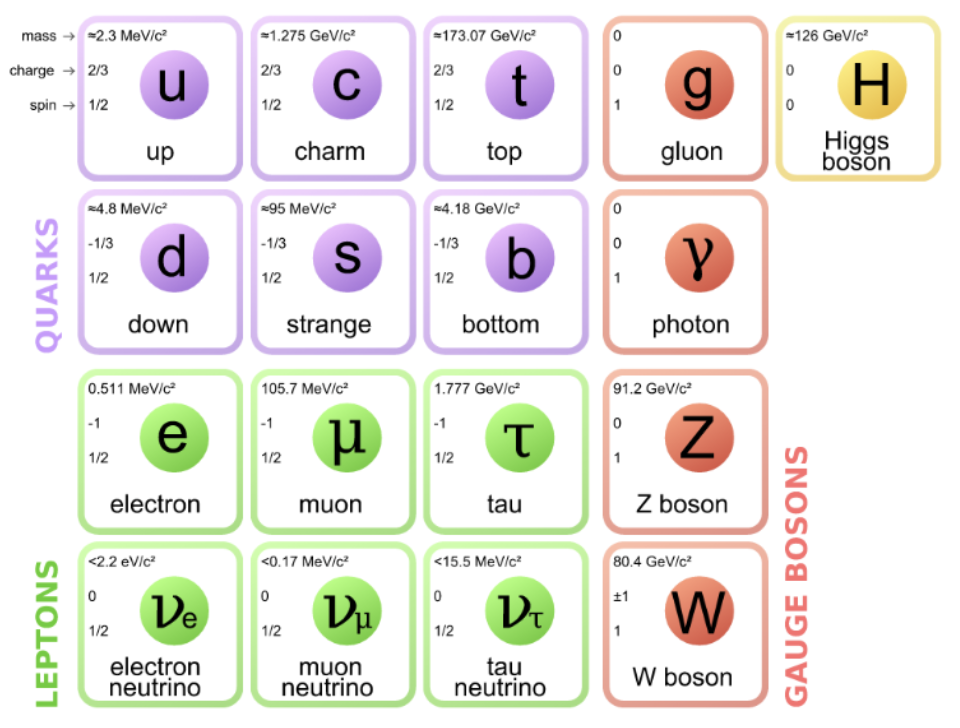
\includegraphics[width=0.8\linewidth]{./Figures/SMChart.png}
	\caption{A chart of all the known irreducible particles of the standard model of particle physics. The three generations of quarks are shown in purple. The three generations of leptons are shown in green. The gauge bosons, which mediate the strong, weak, and electromagentic forces are shown in red. The Higgs boson is shown in yellow.}
	\label{fig:SMOverview}
\end{figure}

In rest of this chapter, Feynman diagrams will be used to represent particle interactions. These diagrams are schematics showing the quanta involved in an interaction (represented as straight, wavy, or curly lines) and intersection points where the interactions occur. By general convention, moving from the right to left of such a diagram corresponds to going forward in time. For particles with a corresponding antiparticle (fermions), an arrow on a line pointing towards the right generally denotes the particle while an arrow pointing towards the left denotes the antiparticle. Generally, quarks are shown as solid lines, bosons such as the photon, W, and Z are shown as wavy lines, gluons are shown as curly lines, and a dashed line is used to represent the Higgs boson.

In order to calculate the amplitudes of an interaction in particle physics, complicated path integrals must be computed. Feynman diagrams introduce so-called Feynman rules, which allow these integrals to be constructed using the diagrams themselves \cite{FeynmanRules}. As a reuslt, Feynman diagrams are an invaluable tool to not only qualitatively understand how particles interact in QFTs but also to construct and calculate the relevant amplitudes necessary for a theoretical understanding of the production and decay of fundamental particles.

\section{Quantum Electrodynamics (QED)}\label{sec:QED}
Quantum electrodynamics was the first successful field theory proposed, and was originally created to describe the phenomena of the electromagnetic forces \cite{SMOverview}. This original theory was built on U(1) gauge symmetry, and thererefore has one generator corresponding to one gauge boson, the photon. In this theory, there is one type of charge: electric charge can either be positive or negative. Interactions in QED occur when a photon couples with any electrically charged fundamental particle. The fundamental interaction of QED is between any charged fermion-antifermion pair and a photon. The fermion ($f$) and antifermion ($\bar{f}$) can be either a quark or a charged lepton, but not an uncharged neutrino.

\section{Quantum Chromodynamics (QCD)}\label{sec:QCD}
The next field theory developed was Quantum Chromodynamics, or QCD. This theory governs the interactions of quarks through the strong nuclear force. Corresponding to an SU(3) gauge symmetry, QCD has 8 generators and therefore 8 force mediators, called gluons \cite{PDGReview}. 

One vital component of QCD is quark confinement. In QED, the electromagnetic force falls of with increasing distance; this fact allows nearby charges to interact, but increasing the separation between the charges is able to weaken the force until the two objects are no longer bound. In contrast, the strong nuclear force actually increases in magnitude as the separation between two color-charged particles increases \cite{SMOverview}. So, as two quarks are separated from eachother, the bond between them contains more and more energy. As the separation grows larger and larger, there comes a point where the energy stored in the gluons binding the quarks together is larger than the energy required to produce a new quark-antiquark pair. 

Quark confinement leads to the production of what are termed QCD jets \cite{PDGReview}. 

\section{Electroweak (EW) Theory}\label{sec:EW}
The weak nuclear force was originally formulated by Enrico Fermi in 1938 as a way to explain the process of beta decay of nuclei \cite{FermiWeakPaper}. While this force was originally proposed as the 4th fundamental force, it was also not a complete description and was therefore not a major area of study immediately. After QED began to prove highly fruitful, great efforts to formulate the weak interaction as a field theory were undertaken in earnest in the 1950s. Then, between 1959 and 1961, two papers by first Salam and Ward, and then Glashow, proposed a major step forward in formulating the weak force as a field theory \cite{SalamAndWardEW} \cite{GlashowEW}. This breakthrough came in the form of unifying the electromagnetic and weak nuclear forces into one single electroweak theory. 

By combining the SU(2) gauge symmetry of the weak force with the U(1) symmetry of QED, a new group with total symmetry SU(2)xU(1) can be formulated \cite{PDGReview}. 



\section{The Higgs Field and Higgs Boson}\label{sec:Higgs}
\subsection{Properties of the Higgs Potential}
\begin{equation}\label{eqn:HiggsPotential}
    V(\phi) = frac{1}{2}m^2_H\phi^2 + sqrt{\lambda/2}m_H\phi^3 + frac{1}{4}\lambda\phi^4
\end{equation}

\subsection{Production Modes of a Single Higgs Boson}\label{sec:SingleHProdModes}
With the establishment of the existence of the Higgs boson, both the production and decay modes of the particle must be studied and measured. The production modes are all of the theoretically-allowable ways in which a Higgs boson may be created. Determining which modes are allowable is a complicated process of using the relevant quantum field theories (QCD and EW theory for the Higgs boson) to constrain possible interactions using the conservation laws of each theory.

The primary production modes for the Higgs boson are all shown as feynman diagrams in figure \ref{fig:FDSingleHProdModes}, reproduced from \cite{CMS10YearReview}. Figure \ref{fig:FDSingleHProdModes}a shows what is called gluon fusion (ggH), where two gluons directly fuse through a virtual (top or less commonly bottom) quark loop. It can immediately be seen that this ggH production mode does not produce any additional particles from the primary interaction. The next mode, in figure \ref{fig:FDSingleHProdModes}b is known as Vector Boson Fusion (VBF). This occurs when two quarks each radiate a vector boson (either $W^{\pm}$ or $Z^0$). These vector bosons then interact, and can produce a Higgs boson. VBF production also only produces a single Higgs boson, with the other two outgoing particles simply being the recoiling quarks that originally produced the vector bosons.

The other Higgs production modes shown are called associated production modes; instead of simply combining the energy of two particles together to produce a single Higgs boson, associated production modes create the Higgs in conjunction with some other particle. In figure \ref{fig:FDSingleHProdModes}c, vector boson associated production is shown. In this mode, two quarks directly interact to create a vector boson, which then branches into a Higgs in associated with an additional vector boson. For this process, that vector boson may be either a $W^{\pm}$ or $Z^0$. The next diagram, shown in figure \ref{fig:FDSingleHProdModes}d, is the production of the Higgs in association with a quark pair, either the top or bottom quark. These are termed ttH or bbH production, and often produce considerable background given the jets of hadronic particles that originate from the top or bottom quarks. The final two diagrams, \ref{fig:FDSingleHProdModes}e\&f, are the production of a Higgs in association with a single top quark. 

\begin{figure}[H]
	\centering
	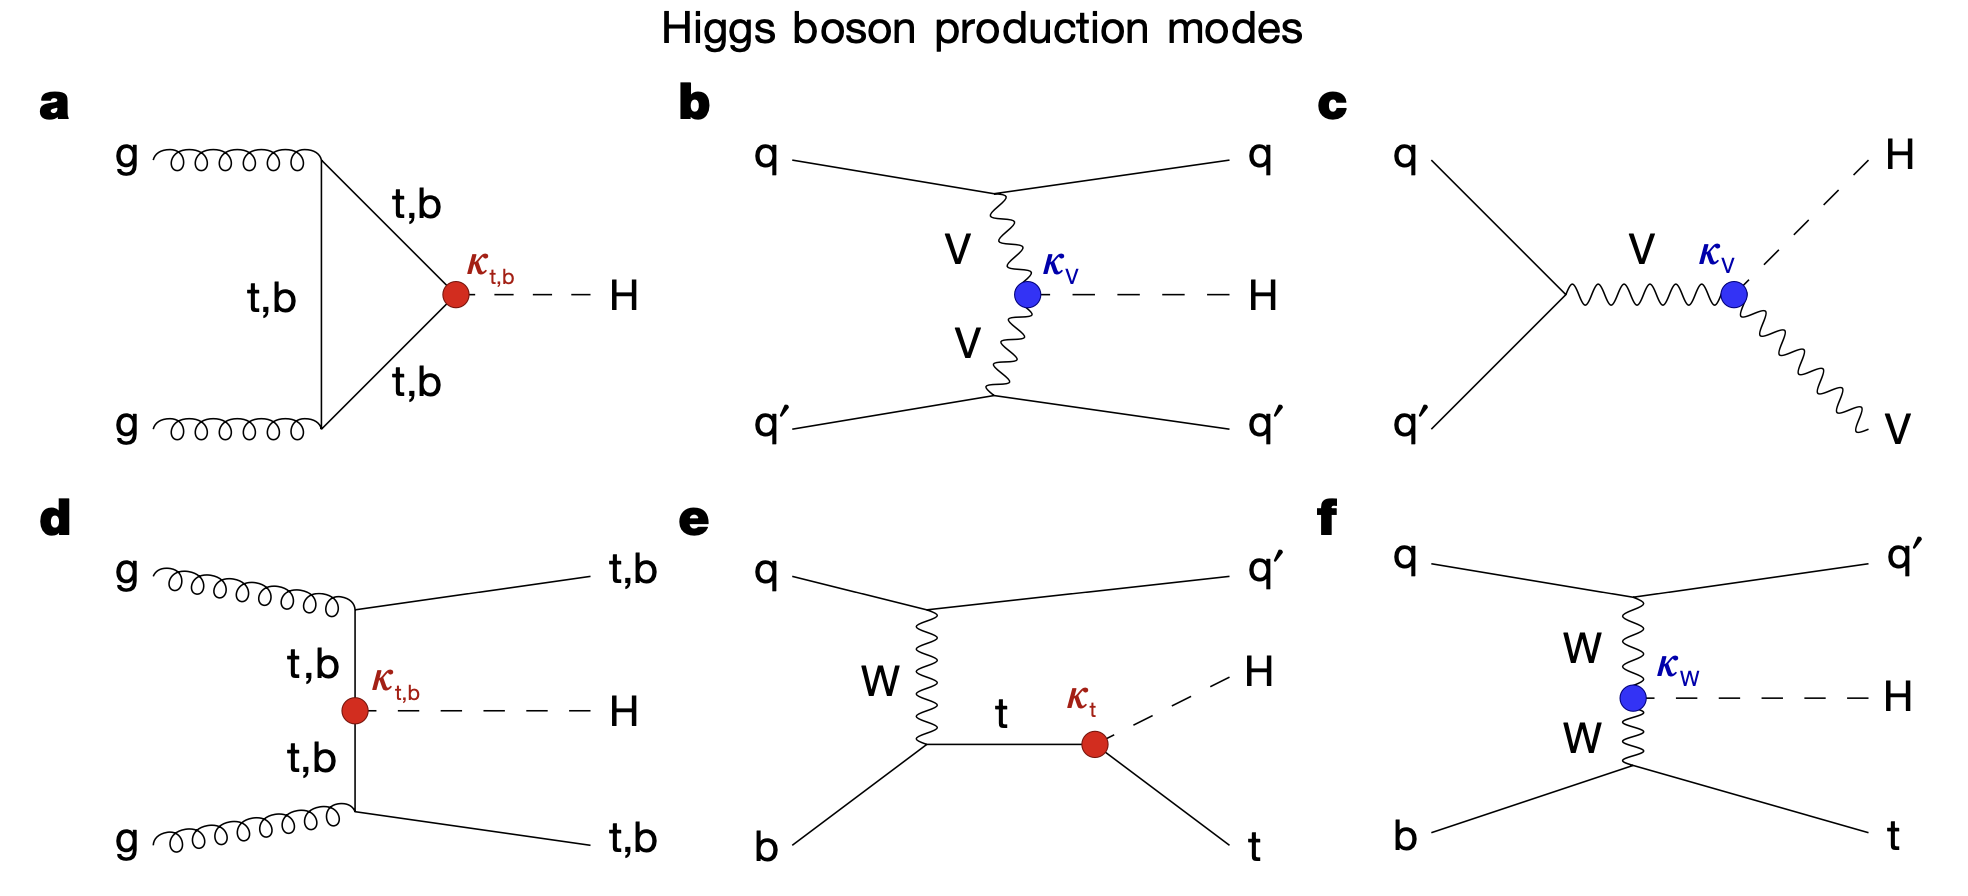
\includegraphics[width=\linewidth]{./Figures/HiggsProdModes_From10YearReview.png}
	\caption{Feynman diagrams of known Higgs production modes. a is known as gluon fusion, termed ggH. b is known as vector boson fusion (VBF). c is production of the Higgs in association with a vector boson (either a $W^{\pm}$ or $Z^0$ boson), called VH production. d is the production of the Higgs in association with a pair of top (ttH) or bottom (bbH) quarks. e and f both show Higgs production in association with a single top quark (tH). Reproduced from \cite{CMS10YearReview}}
	\label{fig:FDSingleHProdModes}
\end{figure}

Of note are the factors placed at each of the vertices in these diagrams. Coupling parameters are part of the field-theoretical matrix element calculations, and are a factor placed at each vertex of a particular particle combination. In experimental measurements, however, the coupling parameters are generally measured as coupling modifiers, denoted by $\kappa$, which are the ratio of the measured coupling parameter to the SM prediction for its value \cite{CMS10YearReview}. For the coupling of a Higgs and a top quark, for example, a value of $\kappa_t = 1$ would mean that the measured coupling parameter exactly matches that predicted by the standard model. The measurement of the coupling parameters is a major goal of the Higgs physics program at the LHC. As can be seen in figure \ref{fig:FDSingleHProdModes}, vertices on these diagrams are labeled with the relevant coupling modifiers. In red are Higgs-quark couplings, $\kappa_t$ for top quarks and $\kappa_b$ for bottom quarks. In blue are bosonic couplings, $\kappa_V$ for a general vector boson, and $\kappa_W$ for a $W^{\pm}$.

Not all allowed production modes are of equal probability, however; each possible mode has an associated cross-section, represented by $\sigma$. This cross-secton is generally measured in a unit of area called a picobarn (pb), where one picobarn is equal to $10^{-36} cm^2$. The cross-section depends on the total center-of-mass collision energy, $\sqrt{s}$ (measured in units of energy, in this case teraelectronvolt {TeV}). At a center of mass energy of $\sqrt{s} = 13$TeV, recent results have shown the total Higgs boson production cross section as $\sigma_H = 54 \pm 2.6$pb \cite{HiggsCrossSection}. Gluon fusion production accounts for about 87\% of this total cross-section \cite{CMS10YearReview}. Taken together with the next most common mode, VBF, over 93\% of the total cross-section can be accounted for. The cross-section for different production modes are tabulated in table \ref{tab:singleHProductionXS}. The proportions are represented in the pie chart shown in figure \ref{fig:XSSingleHProdModes}, reproduced from \cite{CMS10YearReview}.

\begin{table}
	\centering
	\caption{Table showing the calculated cross-sections (in pb) of the single Higgs boson production modes for $\sqrt{s} = 13$TeV. This data has been taken from \cite{HiggsCrossSection}.}
	\label{tab:singleHProductionXS}
	\begin{tabular}{c c} 
		\hline
		\textbf{Production Mode} & \textbf{Cross-section (pb)} \\
		\Xhline{2pt}
		ggH & 48.31 $\pm$ 2.44\\
		VBF & 3.771 $\pm$ 0.807\\
		WH & 1.359 $\pm$ 0.028\\
		ZH & 0.877 $\pm$ 0.036\\
		ttH & 0.503 $\pm$ 0.035\\
		bbH & 0.482 $\pm$ 0.097\\
		tH & 0.092 $\pm$ 0.008\\
		\hline
	\end{tabular}
\end{table}

\begin{figure}[H]
	\centering
	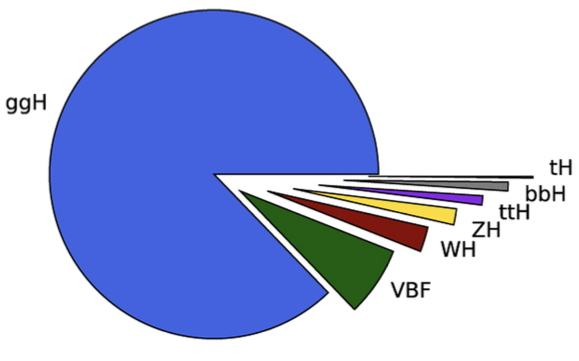
\includegraphics[width=0.75\linewidth]{./Figures/SingleHProdXSPieChart.png}
	\caption{A pie chart of the relative proportions of the total $\sigma_H$ attributed to each production mode. Reproduced from \cite{CMS10YearReview}.}
	\label{fig:XSSingleHProdModes}
\end{figure}

\subsection{Decay Modes of a Single Higgs Boson}\label{sec:SingleHDecayModes}
While section \ref{sec:SingleHProdModes} covers the ways to create a Higgs boson at the LHC, the ways in which the Higgs decays are of even more vital importance. With a SM lifetime of $\tau_H = 1.6 \times 10^{-22}$s, the Higgs itself cannot be directly measured \cite{CMS10YearReview}. Instead, the final state particles must be measured and the Higgs reconstructed from them. Feynman diagrams for the possible decay modes are show in figure \ref{fig:SingleHDecayModes}. There are 4 major classes of Higgs decays: vector bosonic decays where the final state is a pair of W or Z bosons (figure \ref{fig:SingleHDecayModes}g); fermionic decays where the final state is a fermion-antifermion pair (figure \ref{fig:SingleHDecayModes}h); photonic decays where the final state is either two photons or a photon and a $Z^0$ boson(figure \ref{fig:SingleHDecayModes}i\&j); and decays into two gluons, which are mediated by a b/t quark loop (not shown in figure \ref{fig:SingleHDecayModes}).
\begin{figure}[H]
	\centering
	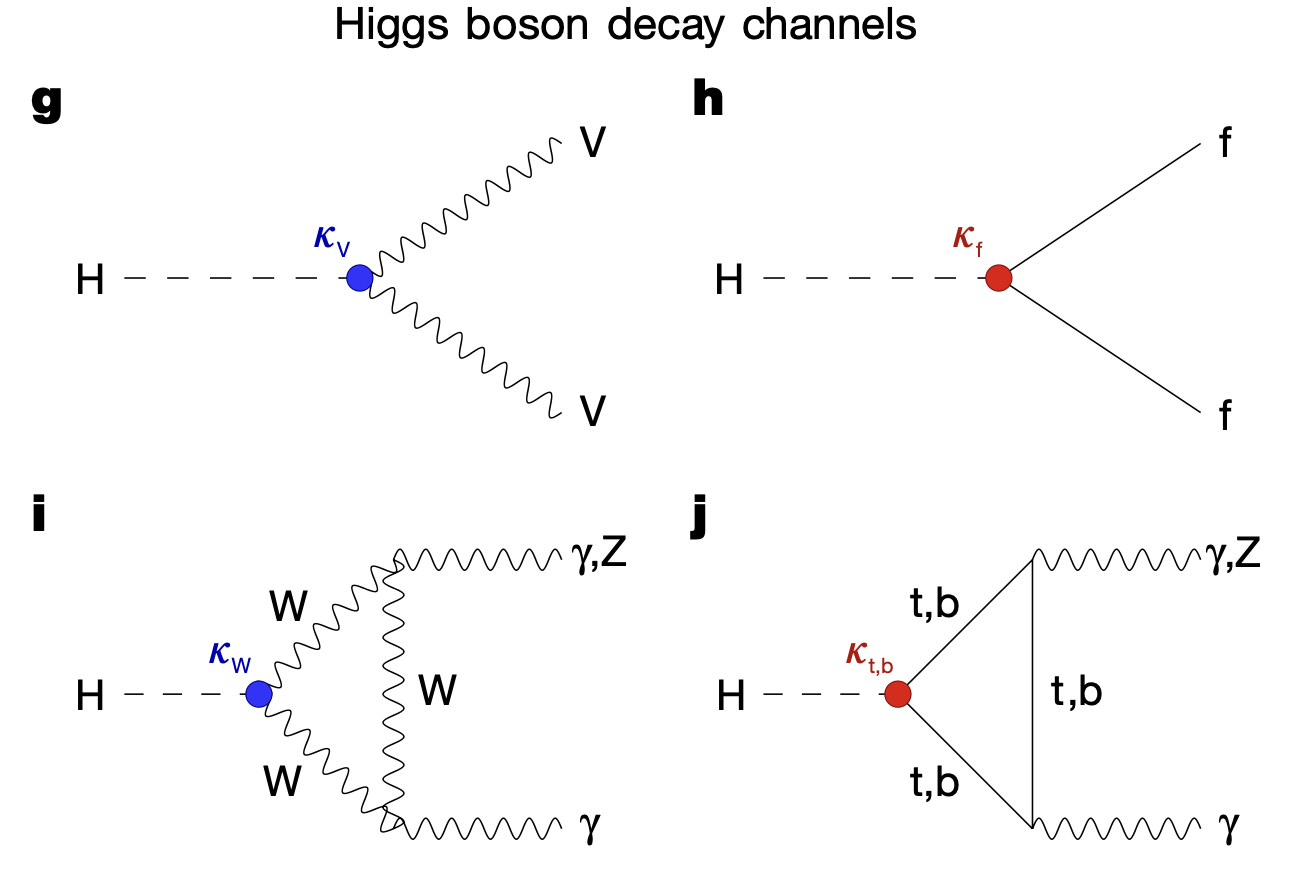
\includegraphics[width=\linewidth]{./Figures/HiggsDecayModes_From10YearReview.png}
	\caption{Feynman diagrams of known Higgs decay modes. Heavy vector bosonic decays are shown in g, fermion-antifermion decays are shown in h, and photon/Z boson decays are shown in i and j. Reproduced from \cite{CMS10YearReview}}
	\label{fig:SingleHDecayModes}
\end{figure}

As with the production modes, not all of the decay modes are equally likely. Whereas a production mode is assigned a physical cross-section, a decay mode is described by the branching faction, which quantifies what percent of all produced particles will decay through a certain channel. These branching fractions, as with the production cross-sections, can be both theoretically calculated and measured from experiments. Table \ref{tab:singleHDecayBR} shows the branching fractions of the main Higgs decay modes with information obtained from \cite{HiggsCrossSection}. The total fractions are also shown as a pie chart in figure \ref{fig:BRSingleHDecayModes}, which has been reproduced from \cite{CMS10YearReview}.
\begin{table}
	\centering
	\caption{Table showing the theoretical branching fractions of various Higgs decay channels at $\sqrt{s} = 13$TeV. This data has been taken from \cite{HiggsCrossSection}.}
	\label{tab:singleHDecayBR}
	\begin{tabular}{c c} 
		\hline
		\textbf{Decay Channel} & \textbf{Branching Fraction (\%)} \\
		\Xhline{2pt}
		b$\bar{b}$ & 57.63 $\pm$ 0.70\\
		WW & 22.00 $\pm$ 0.33\\
		gg & 8.15 $\pm$ 0.42\\
		$\tau \tau$ & 6.21 $\pm$ 0.09\\
		cc & 2.86 $\pm$ 0.09\\
		ZZ & 2.71 $\pm$ 0.04\\
		$\gamma \gamma$ & 0.227 $\pm$ 0.005\\
		Z$\gamma$ & 0.157 $\pm$ 0.009\\
		ss & 0.025 $\pm$ 0.001\\
		$\mu \mu$ & 0.0216 $\pm$ 0.0004\\
		\hline
	\end{tabular}
\end{table}

\begin{figure}[H]
	\centering
	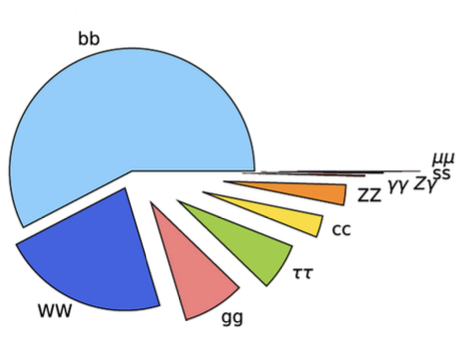
\includegraphics[width=0.75\linewidth]{./Figures/SingleHBRPieChart.png}
	\caption{Theoretical branching fractions for a single Higgs. Reproduced from \cite{CMS10YearReview}}
	\label{fig:BRSingleHDecayModes}
\end{figure}

As seen in the table, the b$\bar{b}$ decay channel is by far the most likely for the Higgs boson. This channel therefore will be produced at high rate at the LHC. The b quarks, however, will produce many hadronic jets as described in \ref{sec:QCD}. So, while this decay is very high-rate, it can be quite hard to measure reliable due to the preponderance of produced particles. The WW (heavy vector boson) decay is the next most common. These bosons most often decay into a 4 lepton final state, which can be hard to disentangle from the possible sources of background. Additionally, if not all 4 leptons are correctly identified, the event may be very hard to reconstruct. Together, these two high-rate but less clean signal signatures make up more than 75\% of the total branching fraction for single Higgs decay.

\section{Higgs Boson Decaying to Two Photons ($H \rightarrow \gamma\gamma$) }\label{sec:HiggsToGammaGamma}
For this analysis, the major decay channel of interest will be the diphoton, or $\gamma \gamma$ decay. This is, again, represented by the Feynman diagrams in figure \ref{fig:SingleHDecayModes}i\&j. Looking at table \ref{tab:singleHDecayBR} and figure \ref{fig:BRSingleHDecayModes}, it is clear that this decay channel has a very low branching fraction compared to some of the higher-rate channels at only 0.2\%. Its major advantage, however, comes from the purity of signal. As discussed in section \ref{sec:QCD}, pp scatting processes produce a nearly uncountable number of QCD jets. So, any final state where jets are expected can be very hard to separate from the backgrounds at play. Additionally, individual jets can contain dozens to hundreds of individual signatures, and are therefore very challenging to reconstruct with high accuracy.

Diphoton decays sidestep many of these issues with QCD-like decay channels. While there will be many background photons, their rate is considerably lower than that of jets. Additionally, photon signatures are relatively well-resolved and much easier to properly reconstruct than jet signatures. As will be discussed in section \ref{sec:HLTReco}, photon signatures tend to be well-columnated and more likely to be isolated from other signatures. Additionally, since the CMS detector places the detector element that measures photon signatures closer to the particle interaction point, photons tend to spread out less than QCD jets and produce fewer additional particles for each real signature. So, then, the $H \rightarrow \gamma \gamma$ has always proven to be a very fruitful Higgs decay despite its low rate.

\subsection{Historical Results}
\section{Di-Higgs Production and Properties}
Another major area of investigation are in diHiggs production modes. One major benefit of such analyses is the ability to probe the Higgs self-coupling, $\lambda$, introduced in equation \ref{eqn:HiggsPotential} \cite{CMS10YearReview}. Since both $m_H$ and $\lambda$ are free parameters in the BEH potential, experimentally constraining both $m_H$ and $\lambda$ would allow for a more complete picture of the overall BEH field. This process provides one way to probe possible beyond standard model physics, as a better understanding of the BEH field may point fundamental physics in a new direction.

As with single Higgs physics, DiHiggs processes can be understood in terms of their production and decay modes. There is no additional physics to be found in DiHiggs decays; once the two independent Higgs bosons are produced, they both decay exactly according to the decay modes described in section \ref{sec:SingleHDecayModes}. The possible Higgs boson pair production modes, however, are of considerable interest. As opposed to the variety of possible production modes for the single Higgs, diHiggs modes come in one of two flavors: ggH and VBF. 

\subsection{Di-Higgs Production Modes}
There are two ggH processes, shown in figure \ref{fig:DiHiggsProdModes}k\&l. The first, k, shows the creation of a virtual Higgs, $H^*$, through the same standard top/bottom quark loop as the single Higgs ggH process. This virtual Higgs then decays into two further on-shell (real) Higgs bosons. This process has a tri-linear Higgs coupling vertex, allowing the direct probing of the Higgs self-interaction, $\kappa_{\lambda}$. The second ggH process does not have this tri-linear coupling, instead having a 4-part virtual top/bottom quark loop where one Higgs is produced at each of the forward corners. 

There are three separate VBF modes for DiHiggs production. The first, m, involves the fusion of two vector bosons, then the creation of a virtual $H^*$ which then decays into two final state Higgs bosons. As a result, this production moode probes both $\kappa_{\lambda}$ and $\kappa_V$. The next diagram, n, follows the same process but skips the virtual Higgs. Instead, two Higgs bosons are produced directly at the interaction vertex between the two vector bosons. This introduces a new coupling modifier, $\kappa_{2V}$. The final diagram in o consists of the exchange of a vector boson, leading two two individual $\kappa_V$ vertices. 

\begin{figure}[H]
	\centering
	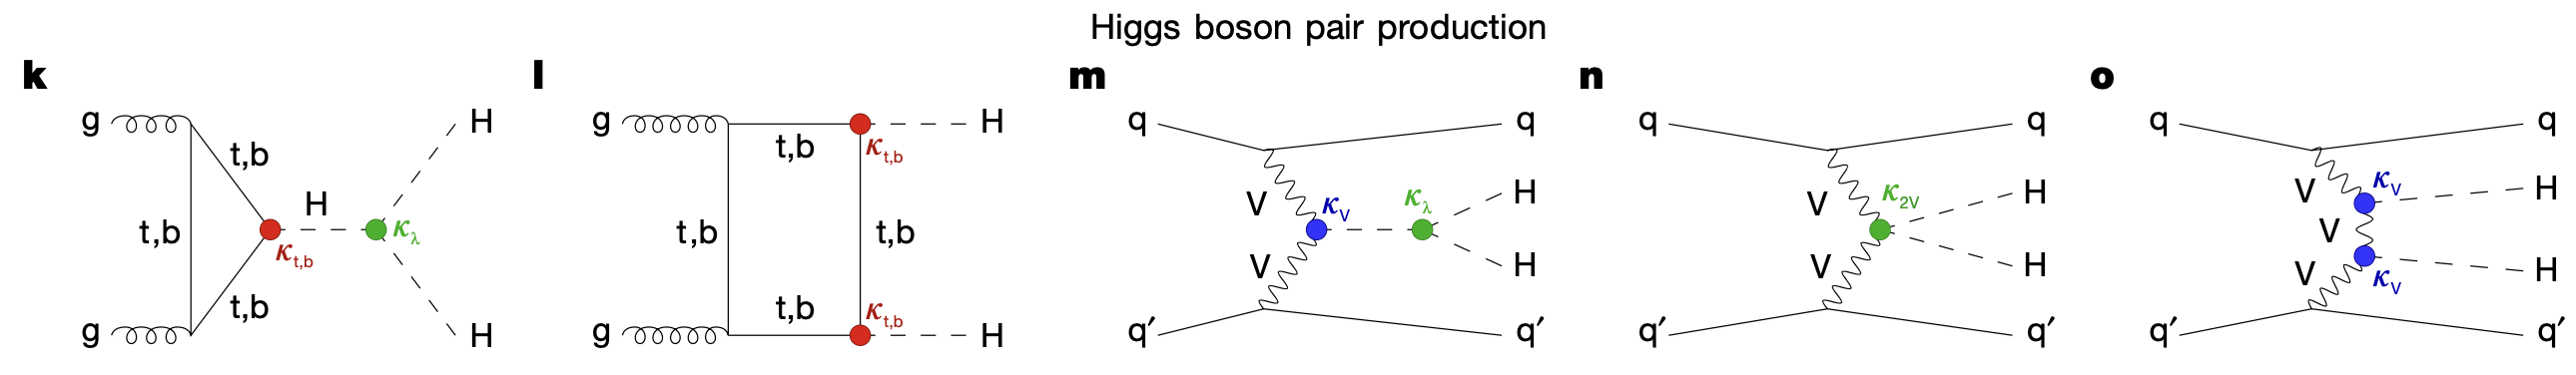
\includegraphics[width=\linewidth]{./Figures/DiHiggsProdModes_From10YearReview.png}
	\caption{Feynman diagrams of known DiHiggs production modes. Figures k and l correspond to the two methods of ggH production, and m,n, and o correspond to the three methods of VBF production. Reproduced from \cite{CMS10YearReview}.}
	\label{fig:DiHiggsProdModes}
\end{figure}

When calculating the scattering amplitudes for DiHiggs production, an interesting phenomenon occurs. The ggH production modes, which are the two most common, actually produce amplitudes of similar magnitude but opposite signs \cite{CMS10YearReview}. So, constructive interference between the amplitudes occurs. This leads to a very small total production cross-section. In fact, whereas the single Higgs production cross section is about $\sigma_H = 54$ pb, the theoretical HH cross-section is calculated to be $\sigma_HH = 32.76 \substack{+1.95 \\ -6.83}$ fb, where a femtobarn is 1/1000th the size of a petabarn. So, then, HH processes are theoretically more than a factor of 1000 more rare than single Higgs processes. As a result, no conclusive results of their measurement have been achieved for Run 2 or Run 3 of the LHC \cite{CMS10YearReview}.

\subsection{The $HH \rightarrow b\bar{b}\gamma\gamma$ Channel}\label{sec:HH2b2g}

Given the incredibly low expected rate of HH production as mentioned in the previous section, all possible pains must be taken to maximize the signal efficiency for relatively high-rate decays of diHiggs production. The $H \rightarrow \gamma \gamma$ decay is still useful for single Higgs production -- as discussed in section \ref{sec:HiggsToGammaGamma} -- because even though it has a relatively low rate, single Higgs production is common enough that the ease of separating the signal from background is a worthwhile tradeoff. That same logic doesn't hold for HH production however; since 0.2\% of single Higgs decay to two photons, only 0.004\% of HH productions would decay to four photons. 

In order to get around this low rate but still take advantage of the ease of identifying $H \rightarrow \gamma\gamma$, the decay $HH \rightarrow \bar{b}b$ can be used. $H \rightarrow \bar{b}b$ has a branching fraction of 57.63\%, but can be quite hard to separate from background given its jet-jet final state. Combining this higher-rate process, however, with the much more easy to disentangle $H \rightarrow \gamma\gamma$ process, however, provides the best possible compromise between rate and ease of identification. 

\chapter{The LHC and CMS Detector}
\section{The Large Hadron Collider}
The Large Hadron Collider, which replaced the prexisting Large Electron-Positron Collider, was constructed between 2000 and 2008. Designed to reach new energy fronteirs by colliding protons at up to 14 TeV, the LHC provided particles physicists with their most powerful tool yet to test the Standard Model and beyond. At the most basic level, these proton-proton collisions are achieved by crossing two counter-rotating proton beams at specific points. These counter-rotating beams are accelerated along the 26.7 km circumference of the LHC within a tunnel of 3.7 m internal diameter \cite{LHC2008}. Initial designes proposed two completely separated proton beam pipes, but it became clear that the space requirements of the existing CERN tunnel (constructed for LEP) precluded this possibility. As a result, a "two-in-one" superconducting magnet design was adopted that allowed the two beams to be transported in separate magnetic coils sharing the same mechanical and cryostat space.

The details of the physical construction of the LHC will be given below in section \ref{sec:LHCDesign}. Of greater importance, however, are the details of how the proton beams themselves collide, and the various measurements and useful quantities defined therein. In section \ref{sec:Collisions}, many details of the proton-proton will be expounded. This section will define several vital concepts that will be of great interest for the future secions of this paper.
\subsection{LHC Design} \label{sec:LHCDesign}
The following section is summarized from \cite{LHC2008}. A simplified schematic of the LHC experiment can be seen in figure \ref{fig:LHCLayout}. As described above, the two proton beams are designed to circulate in opposite directions and interract at specific points along the beams. These two beams can be seen in red (clockwise) and blue (counterclockwise). Of note, there are 4 interaction points, each of which is surrounded by a specific experiment. The ALICE experiment is designed to measure ion collisions. The LHC-B experiment is specifically designed to measured B-physics. The ATLAS and CMS detectors, on the other hand, are designed as complementary general purpose detectors aimed at leveraging the very high production rate of the LHC. While there are major differences in the designs of the two detectors, they were in essence created to attempt to measure similar physical processes. A major advantage to this is reproducability; whenever CMS or ATLAS records a novel result, the other detector can be used to confirm it.

\begin{figure}[H]
	\centering
	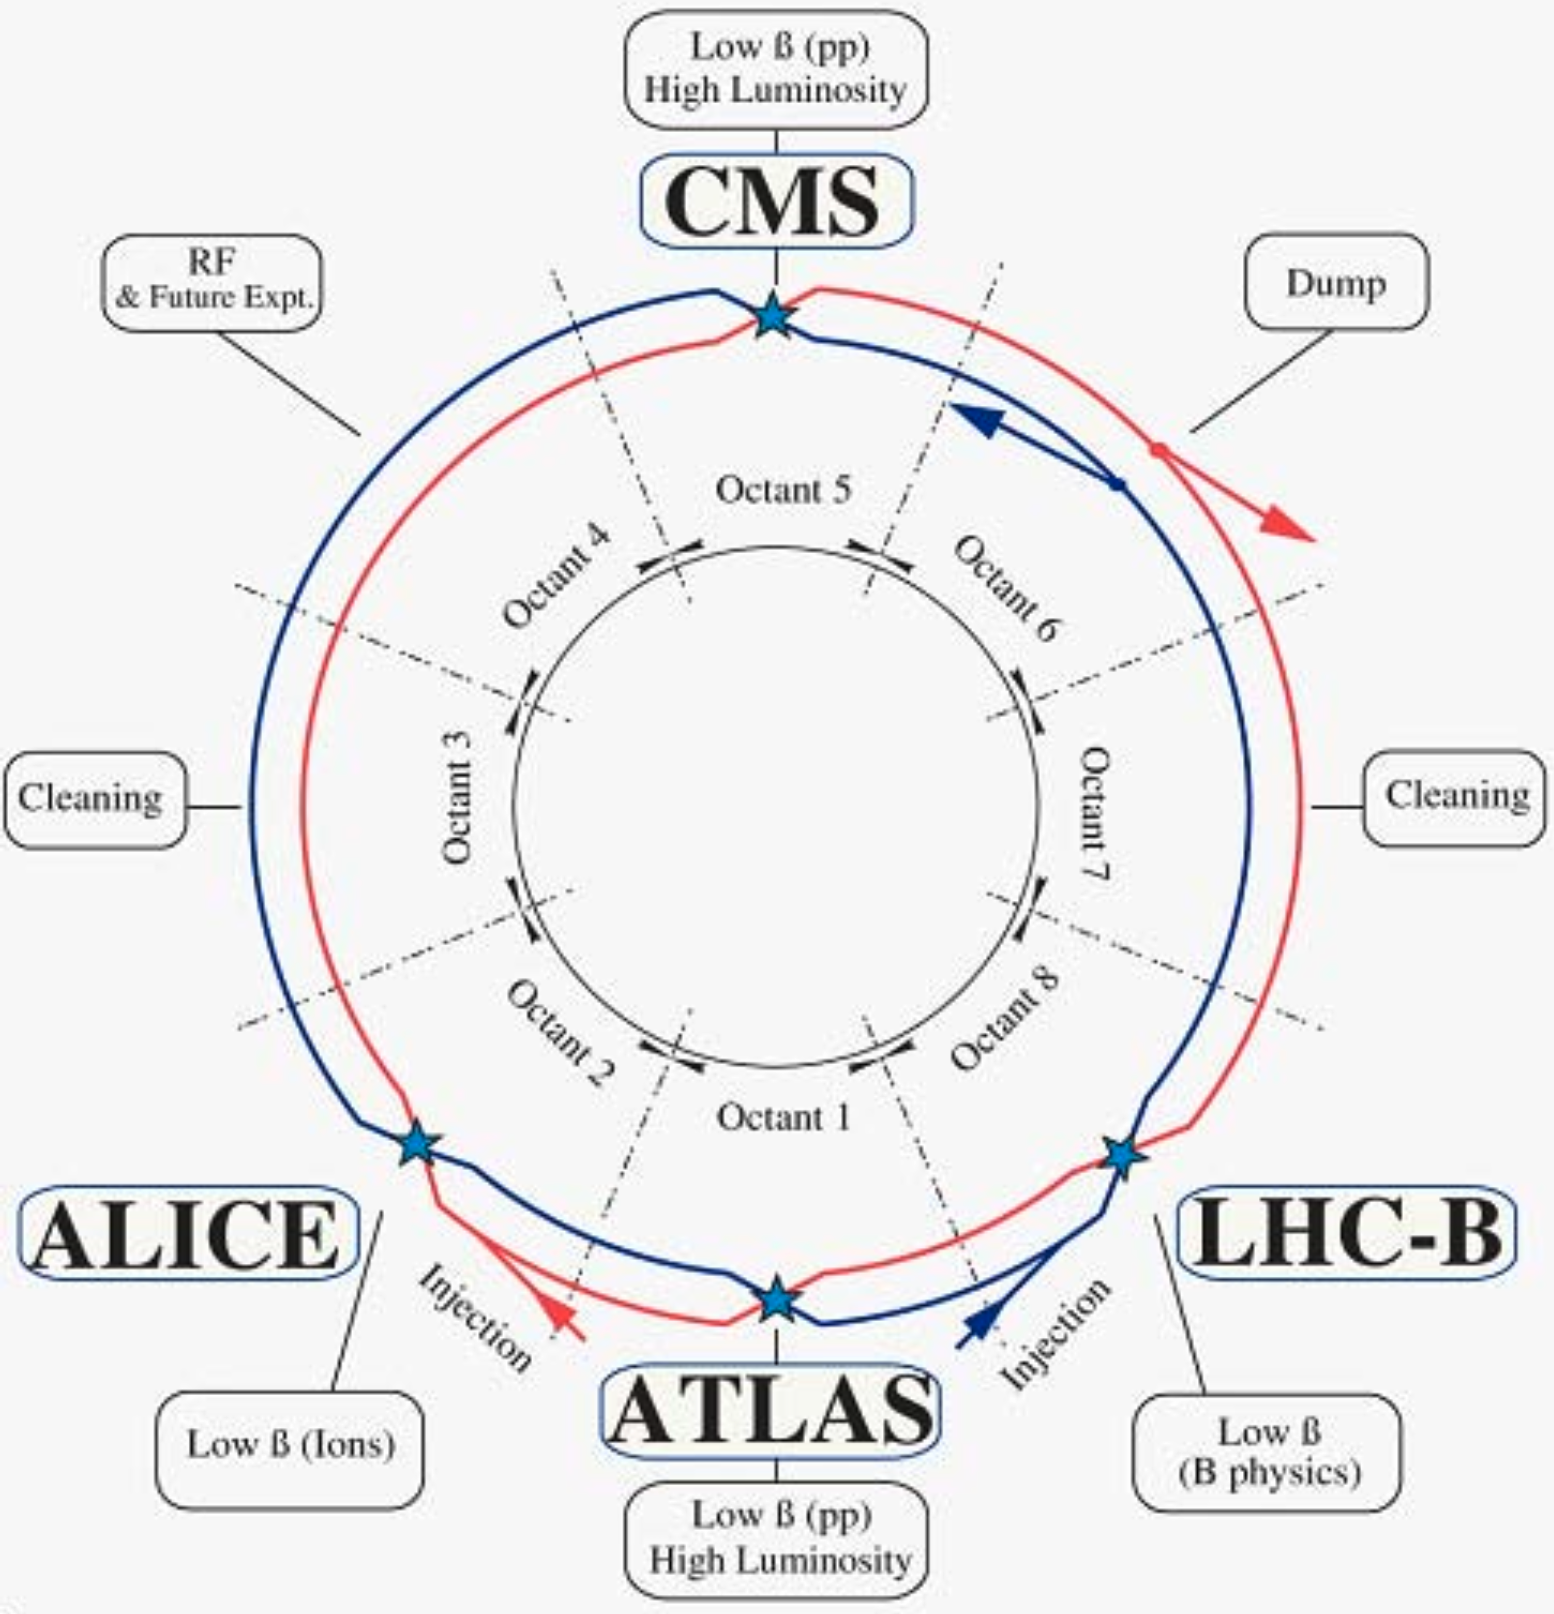
\includegraphics[width=0.75\linewidth]{./Figures/LHCFullLayout.png}
	\caption{A simplified schematic of the overall layout of the LHC. The counter-rotating beams are shown in red (clockwise) and blue (counterclockwise). Reproduced from \cite{LHC2008}. }
	\label{fig:LHCLayout}
\end{figure}

\subsection{Collisions at the LHC} \label{sec:Collisions}
At each of the interaction points shown in figure \ref{fig:LHCLayout}, the proton bunches cross over and the individual protons within each bunch interact with each other. There are two major quantities that define the character of these interactions: center of mass energy and luminosity. Center of mass energy, $\sqrt{s}$, is defined as the total combined energy of both protons in their center of mass frame of refernce (where the two protons are moving in opposite directions at equal speeds). This directly measures how much energy is available to produce additional particles. The original design of the LHC allowed collision energies up to 14TeV, though Run3 at the LHC has only been able to achieve a value of $\sqrt{s} = 13.6$TeV \cite{Run3Hgg2025}. 

The luminosity is a quantity of major concern for physics at the LHC, as it is a measure of the total number of possible collisions in a collider experiment. A higher luminosity value corresponds to more collisions, which corresponds to a higher rate of particle production. The luminosity is measured in two ways. Firstly, the instantaneous luminosity, given in units of $cm^{-2}s^{-1}$, measures the theoretical number of collisions occuring at any given moment. It is defined based on the beam parameters, as shown in equation \ref{eqn:InstLuminosity}.
\begin{equation}\label{eqn:InstLuminosity}
    \mathcal{L}_{inst} = \frac{N^2_b n_b f_{rev} \gamma_r}{4 \pi \epsilon_n \beta^{*}}F
\end{equation}

Here, $N_b$ is the total number of particles per bunch, $n_b$ is the number of bunches per beam, $f_{rev}$ is the revolution frequency, $\gamma$ is the standard relativistic factor, $\epsilon_n$ is the normalized transverse beam emmittance, $\beta^*$ is the beta function at the collision point, and F is the geometric luminosity reduction factor based on the crossing angle of the two beams \cite{LHC2008}. The $\mathcal{L}_{inst}$ is a very useful quantity to understand collisions at the LHC, as it also provides an understanding of the derived quantity termed pileup (PU). Pileup measures the number of total collisions that happen per bunch crossing; when attempting to measure a single signal, a higher PU value will increase the amount of background and extraneous signal events occuring simultaneously. For Run 3, the PU averages about 57 collisions per bunch crossing (REF? LHCP Conference Paper).

Beyond the instantaneous luminosity, a major measure used for considering LHC data is the integrated luminosity, $\mathcal{L}_{int}$ (usually measured in inverse femtobarns, $fb^{-1}$). This is obtained by integrating the instantaneous luminosity over a specific run period. This integration is not as direct as it may seem, however. In reality, the instantaneous luminosity over a specific run decays over time, with a characteristic decay time. This total decay time, $\tau_L$ depends on the losses of protons within the bunch due to collisions, the scattering of particles on residual gasses in the beamline, and IBS scattering effects \cite{LHC2008}. In terms of this characteristic decay time, the total integrated luminosity can be given by equation \ref{eqn:IntLuminosity}.
\begin{equation}\label{eqn:IntLuminosity}
    \mathcal{L}_{int} = L_0 \tau_L \left[ 1-e^{-T_{run}/\tau_L} \right]
\end{equation}

Where $L_0$ is the initial instantaneous luminosity of the run, and $T_{run}$ is the total length of the run. In practice, these quantities are determined by the luminosity group and publicly published for each data sample. Monte Carlo samples are generated with an associated effective luminosity, $\mathcal{L}_{eff}$, which corresponds to the amount of integrated luminosity in the data that would be required to obtain the generated number of signal events.

For any given signal process, as described in chapter \ref{chapter:Theory}, there is a cross section, $\sigma$, which helps calculate the expected number of signal events for that process. These $\sigma$ values are measured in some fraction of a barn, which has units of $10^{-28} m^2$. Generally, cross sections are measured in picobarns (pb) or femtobarns (fb). Immediately, it is obvious that these units are the inverse of the total integrated luminosity. So, then, the expected number of total signal events within a given data period with $\mathcal{L}_{int}$ can be given by equation \ref{eqn:TheoryEvents}.

\begin{equation}\label{eqn:TheoryEvents}
    N^{Tot.}_{event} = \mathcal{L}_{int} \sigma_{event}
\end{equation}

\section{The Compact Muon Solenoid Detector}
This section is largely summarized from \cite{CMS2008} and \cite{CMS2024}. The Compact Muon Solenoid is designed as a 22 m cylinder with a total diameter of 15 m. Centered on the beampipe where a proton-proton bunch crossing occurs, the detector consists of various layers of detector elements designed to track and measure different resultant particles. The general structure of the detector will be described beginning at the center and moving outward. A schematic of the detector can be seen in Figure \ref{fig:FullCMS}. Later sections will provide additional detail on elements of particular interest for our $H \rightarrow \gamma\gamma$ analyses. 

\begin{figure}[h!]
	\centering
	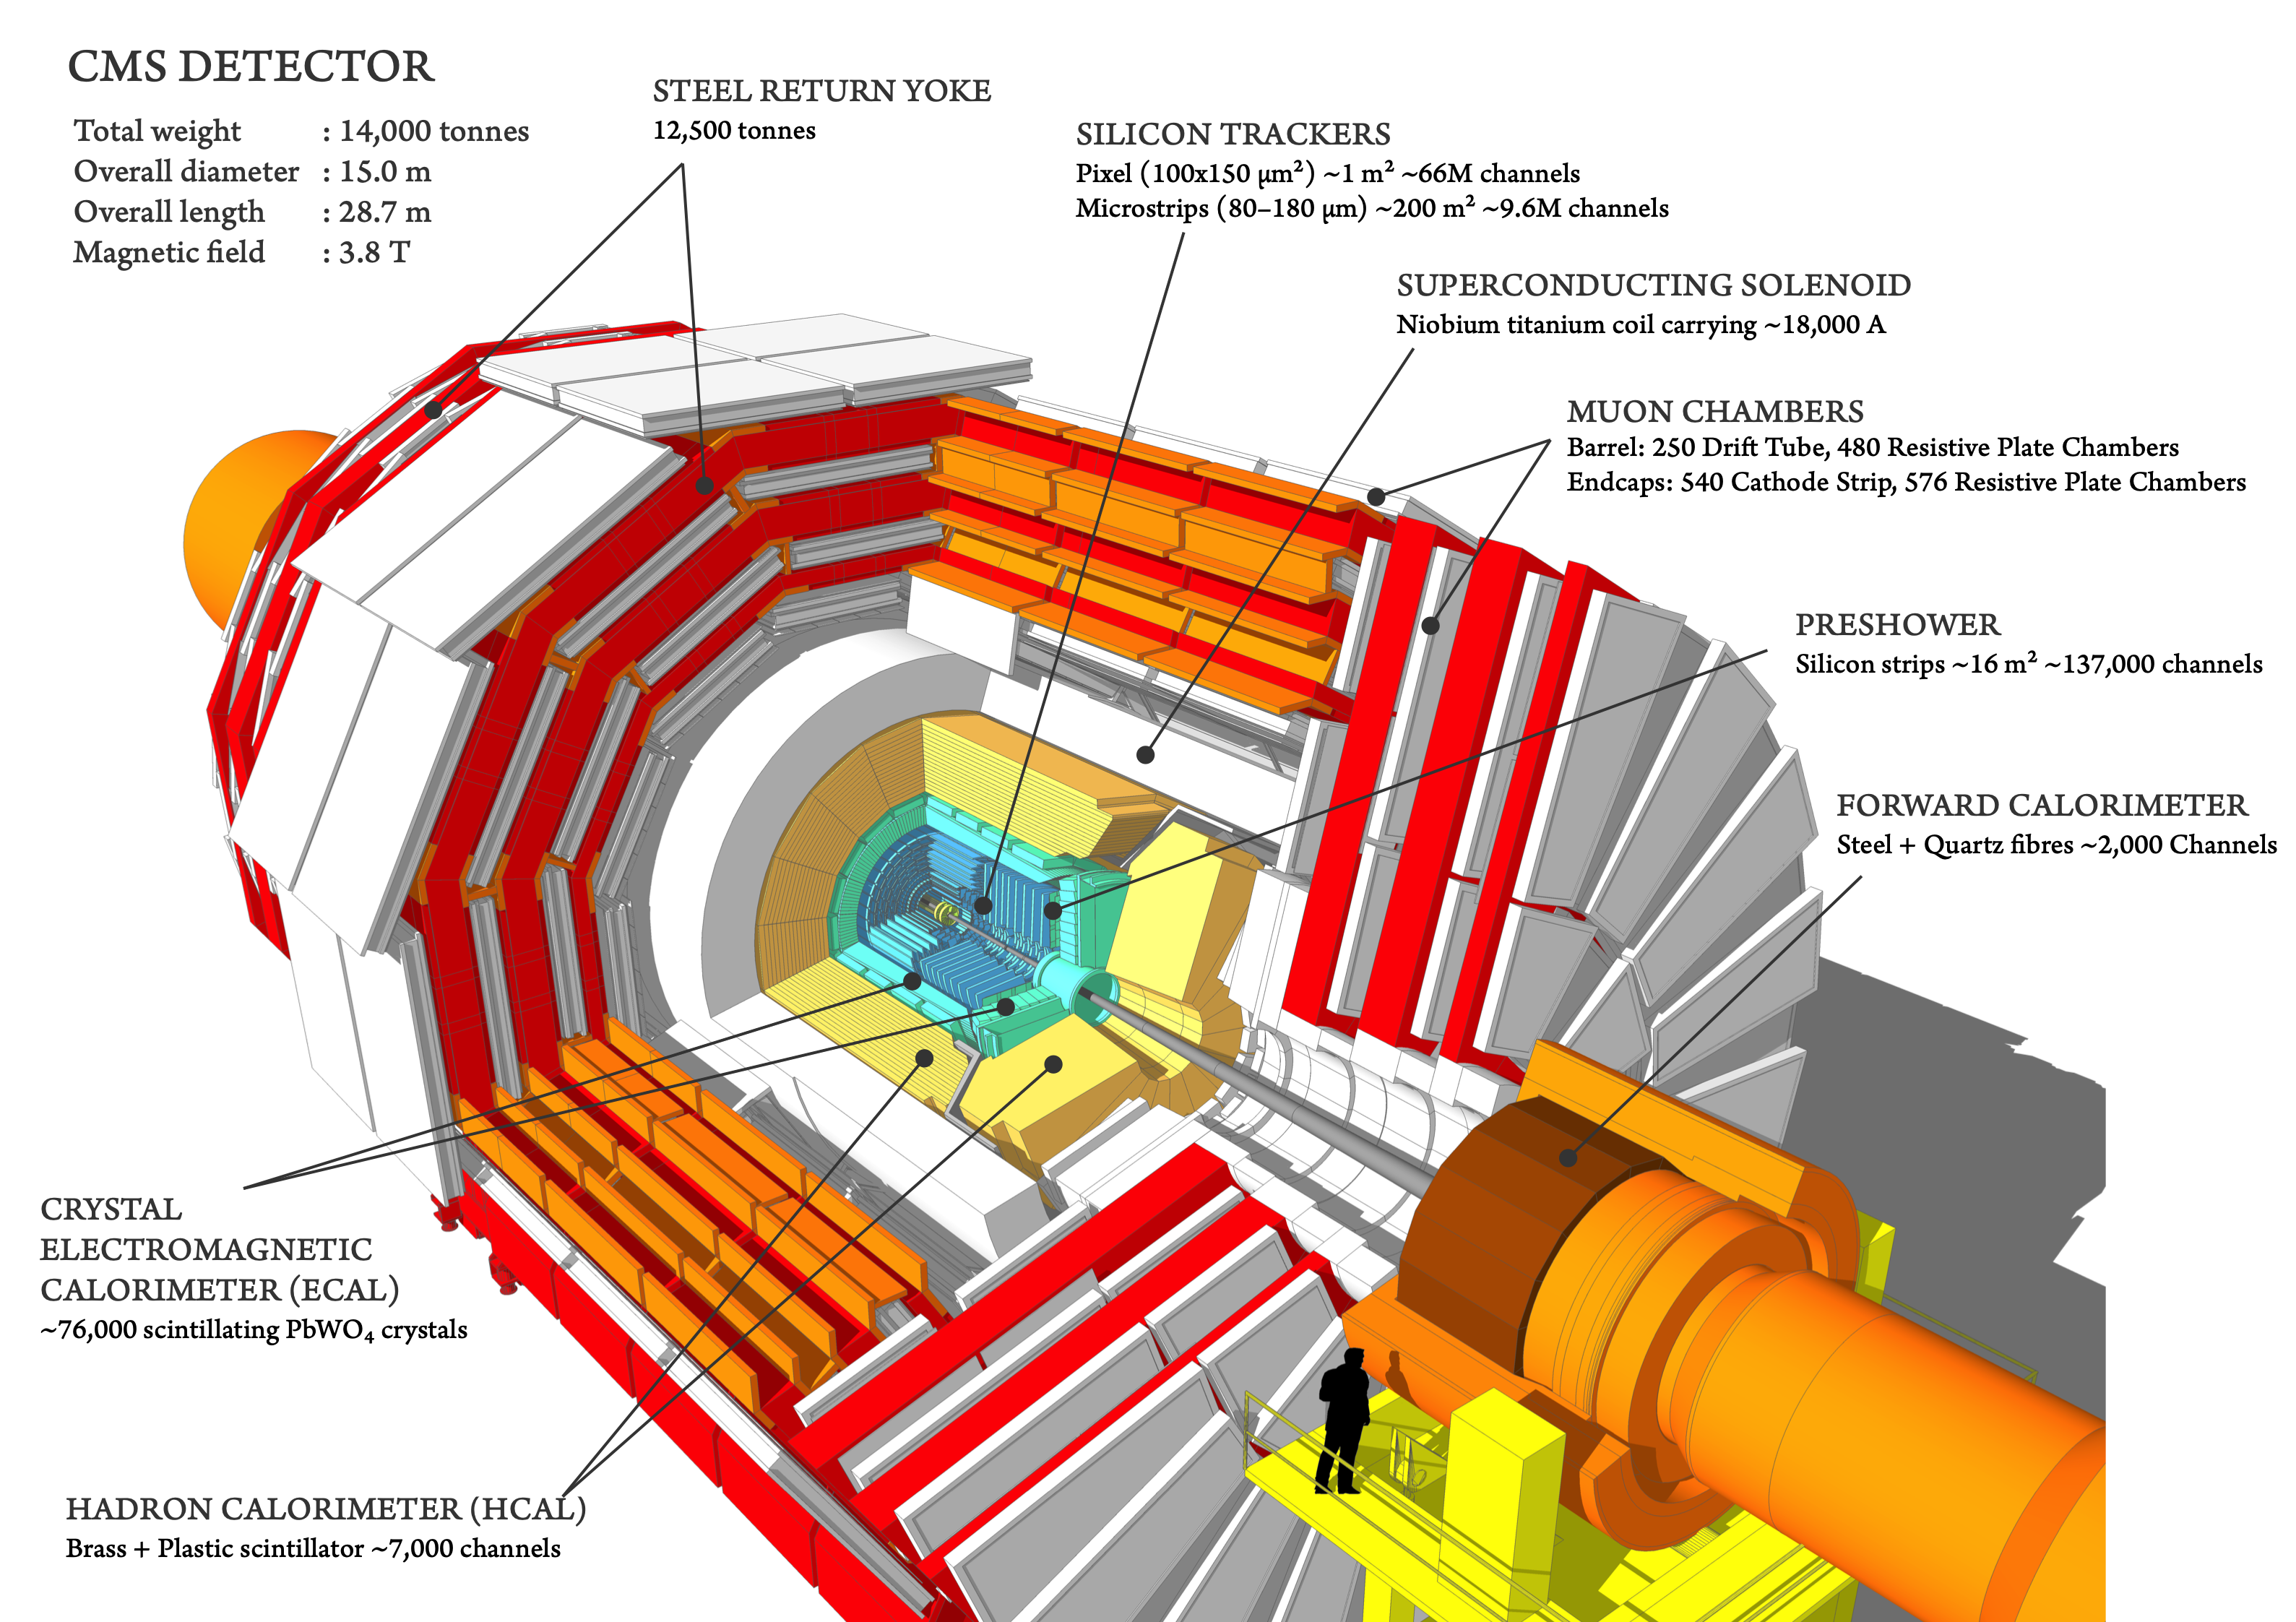
\includegraphics[width=\linewidth]{./Figures/FullCMS.png}
	\caption{A full view of the CMS Detector, with each major system labled. Reproduced from \cite{CMS2024}.}
	\label{fig:FullCMS}
\end{figure}

After particles collide and are scattered, they first interact with the central beampipe that houses the incoming proton bunches. While this element does not provide any detecting capabilities, interactions between the outgoing particles and the material of the beampipe may cause additional scattering and particle production. Next, the particles enter the robust inner tracking system, designed to be able to reconstruct the path of charged particles through the detector. This inner tracking system is composed of an internal pixel detector surrounded by an externam strip detector. These elements will be described in section \ref{sec:InnerTracker}.

The next detector element encountered is the Electromagnetic Calorimeter (ECal), which aims to measure the energies and locations of electrons and photons. Of course, given that the following analysis will be centered on photons, this detector element will be of great interest. This ECal is composed of scintillating $PbWO_{4}$ crystals arranged into both a cylindrical ECal Barrel (EB) concentric with the beamline and two circular ECal Endcaps (EE) oriented orthogonally to the beamline. A Preshower detector is inserted in front of the EE detectors. More details on this detector element will be provided in section \ref{sec:ECal}. 

Further from the beamline, the Hadronic calorimeter (HCal) aims to measure the locations and energies of charged and neutral hadronic particles using plastic scintillator tiles imbeded in a brass volume. Similarly to the ECal, the HCal is composed of a barrel (HB) region and two endcaps (EB). This detector will be described in more detail in section \ref{sec:HCal}. 

A superconducting solenoid encases all three of these internal regions, providing an internal magnetic field of 3.8T. This magnetic field allows the paths of charged particles to be bent, providing more precise measurement of their properties. While vital to the physics of the detector, this solenoid does not contain any detecting elements. Beyond this magnet lies the highly complicated Muon chambers, which will not be described for this anlysis. Close to the beamline but at the ends of the z-axis of the detector lies the forward calorimeter, which will also not be described for this analysis. The entire detector is shrouded in a steel return yoke. 
\subsection{Beampipe and Inner Tracking System} \label{sec:InnerTracker}
A major goal of the CMS detector is to reconstruct the tracks of charged particles. This allows the software to not only track and measure the flight of an individual particle, but it allows the primary interaction vertex (PV) to be measured more accuretely. This is achieved by a two-layerd approach; the pixel detectors closest to the beamline prived high-accuracy three-dimmensiional spatial information on the particles immediately after they leave the beampipe, while the strip detectors are used to reconstruct where the particle went after this precise initial location. Since the analysis of $H \rightarrow \gamma\gamma $ is focused on photons, charged tracks are not expected for the final state particles of interest. This does not mean they are of no use to us, however -- charged tracks can be used to exclude particles from out final state analysis, allowing us to reduce the number of resultant particles and increase the likelihood that the final particles analyzed are photons. 
\subsubsection{Pixel Detector}
The pixel detectors achieve high spatial resolution by using 124 million channels each composed of a single pixel. As with most detector elements at CMS, the pixel detectors are formed by a barrel region (BPIX) and two circular disk endcap regions (FPIX). The barrels use 4 layers of silicon pixels, located at 29, 68, 109, and 160 mm from the beamline. The endcap detectors use 3 layers of pixels, at distances of 291, 396, and 516 mm from the center of the detector along the z-axis.This layout ensures that any charged particle will strike the pixel trackers 4 times at varying distances from the interaction vertex, allowing precise reconstruction of the track starting at the edge of the beampipe. 
\begin{figure}[h!]
	\centering
	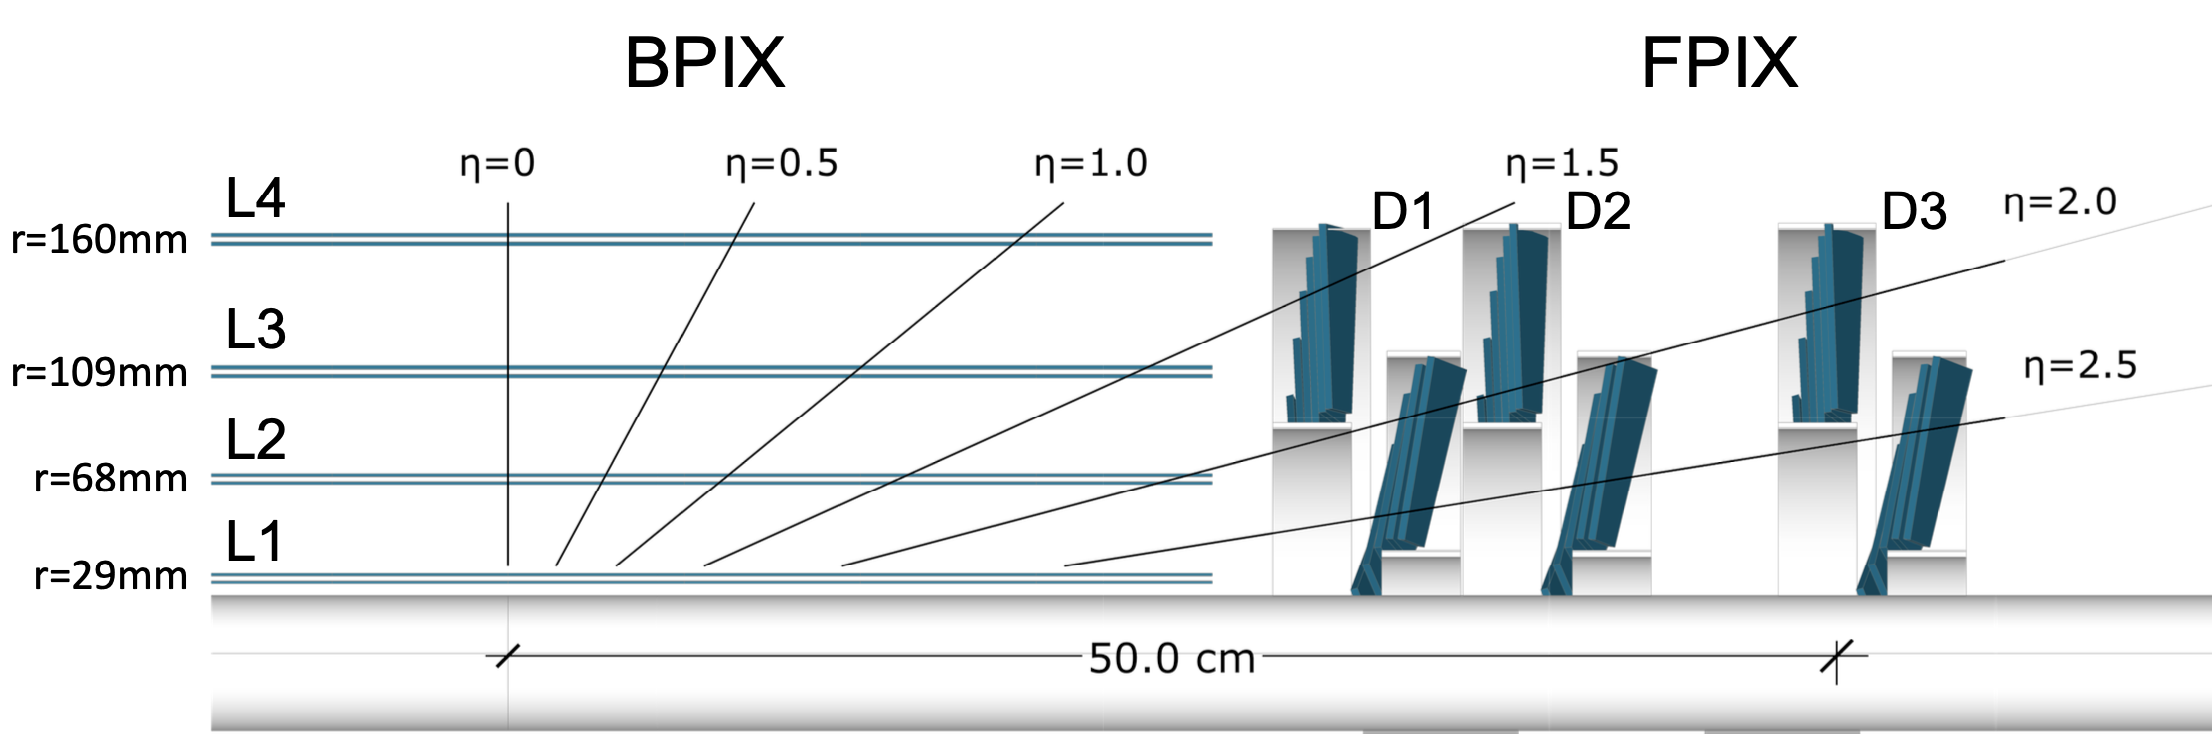
\includegraphics[width=\linewidth]{./Figures/PixelDetector.png}
	\caption{Longitudinal view of the pixel detector, where the beampipe is represented at the bottom of the image. Reproduced from \cite{CMS2024}}
	\label{fig:PixelDetector}
\end{figure}

The individual pixels, of the same size in both the BPIX and FPIX, are housed on sensor modules with 160x416 pixels each (with a total size of 100 x 150 $\mu m^{2}$). This modular structure allows easy replacement of faulty modules, as well as allowing more efficienct production. The BPIX contains 1184 such modules, across its 4 layers, whereas the FPIX contains 672 modules. Light-weight mechanical structures provide the mounting points for these modules, and include cooling aparati. 
\subsubsection{Strip Detector}
The innermost pixel detector is rather small, only extending 160mm radially from the beamline, and 516mm along the beam direction from the interaction point. The majority of the tracking system is composed of the silicon strip tracker (SST). The SST contains 9.3 million silicon micro-strips grouped into 15,148 modules. While there are far fewer channels in the SST, the volume covered is much larger; once the origin of a particle track is pinpointed by the pixel detectors, the strip detectors are able to detect the particle as it travels through a large volume of the detector. The SST has a diameter of 2.5m and a length along the beamline of 5m, so it is clearly a more coarse-grain tracking sensor. 
\begin{figure}[h!]
	\centering
	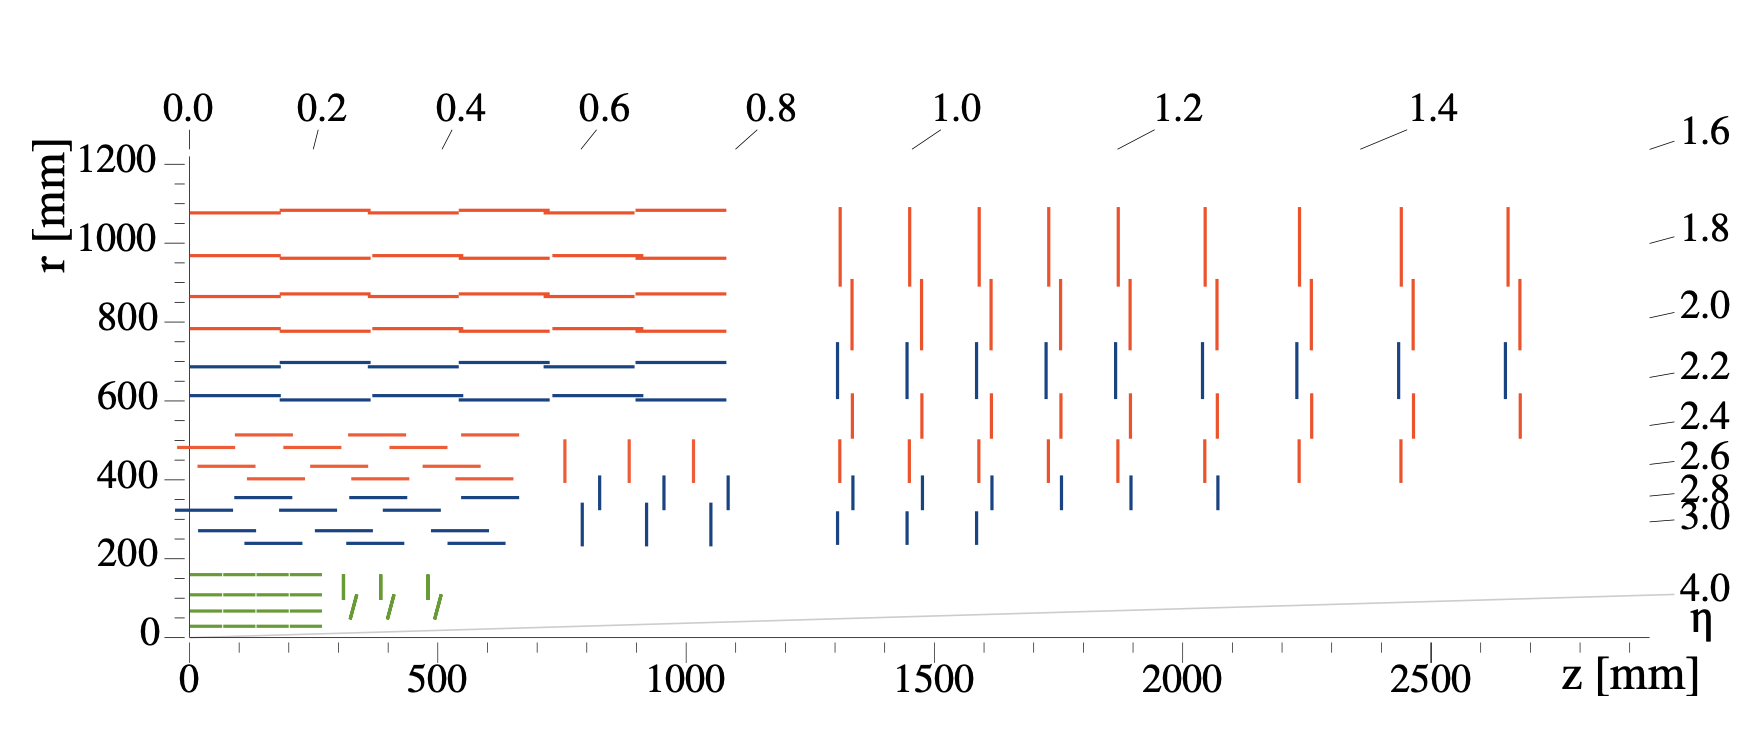
\includegraphics[width=\linewidth]{./Figures/FullTracker.png}
	\caption{Full view of the tracker system. The inner pixel tracker is shown in green. Reproduced from \cite{CMS2024}}
	\label{fig:FullTracker}
\end{figure}
\subsection{Electromagnetic Calorimeter} \label{sec:ECal}
Beyond the inner tracking system, the ECAL system is designed to measure the energies, locations, and arrival times of electrons and photons. A schematic of this detector element can be seen in figure \ref{fig:ECal}, reproduced from \cite{CMS2008}. Given that this paper will be dealing with a two-photon final state, the details of this detector are highly relevant. Similarly to the inner tracker, the ECAL is composed of modules of individual detector elements. Here, however, since the goal is to measure photons and electrons, scintillating material is required. As a result, the individual detector elements are composed of scintillating lead tungstate ($PbWO_{4}$) crystals. These crystals were chosen because, in addition to being optically clear, they are radiaton-hard. Given that the detector will be exposed to high levels of radiation for long continuous stretches, it is imperative that the crystals need not be replaced frequently. The photons from the scintillation of these crystals are detected by photodetectors. The photodetectors differ, however, between the barrel and endcap as explained in detail below. 
\begin{figure}[h!]
	\centering
	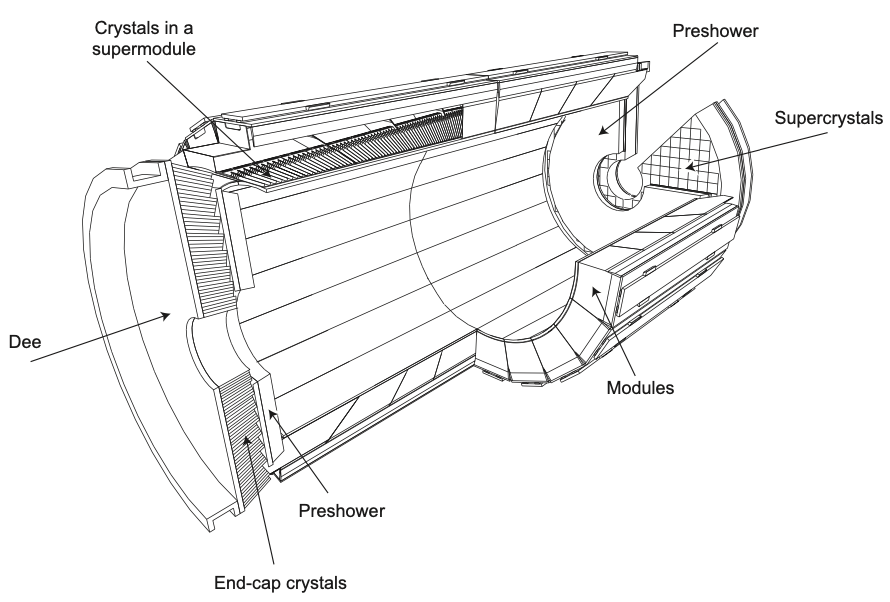
\includegraphics[width=\linewidth]{./Figures/ECalSchematic.png}
	\caption{A simplified schematic of the ECal. Reproduced from \cite{CMS2008}}
	\label{fig:ECal}
\end{figure}

\subsubsection{ECal Barrel (EB)}
The barrel component of the ECAL (EB) is designed, of course, with cylindrical symmetry. In the azimuthal direction, $\phi$, there are 360 crystals per "ring". The barrel detector coveres the pseudorapidity range of $|\eta| < 1.479$, and there are 180 crystals per "row" in this range. As a result, the EB consists of 61,200 total $PbWO_{4}$ crystals. These crystals are tapered, such that the scintillated photons are funneled to the back of the crystal where two avalanche photodiodes (APDs) per crystal collect them. The cross-sectional area of the crystal faces is 22x22 $mm^{2}$. The face of each crystal lies at a distance of 1.29m from the center of the beamline. 

As with the tracker, the individual crystals are combined into submodules and modules, where readout and power-supplying electronics are consolidated. These submodules are of an "aveolar" structure, where the dividing walls between individual crystals ar 0.1mm thick and are made of a combination of alluminum and fibre-epoxy resin. This leads to a total crystal-to-crystal distance of 0.35mm within each submodule. This provides sufficient granularity while still ensuring complete geometric coverage with a reasonable number of individual channels. 
\subsubsection{ECal Endcaps (EE)}
The ECal endcaps (EE) cover the pseudorapidity range of $ 1.479 < |\eta| < 3.0$, and are located symmetrically 315.4cm from the interaction point. The EE is designed as a symmetric disk, with identically shaped crystals grouped in units of 5x5 crystals. The crystals are pointed at a focus point 1300mm beyond the interaction point, meaning that they are angled towards the beam line with an increasing angle (between 2 and 8 degrees) as they move further from the center of the endcap. The cross-sections of these crystals are slightly larger than those in the barrel, measuring at 28.62x28.62 $mm^2$. In total, there are 7,324 crystals for each of the two endcaps laid out in a regular x-y grid. Since this detector element represents much less coverage in terms of area, there are of course fewer total crystals. The difference in the crystal sizes and arrangements relative to the EB means that many of the geometric quanities measured by later reconstructions will differ in the EE.  
\subsection{Hadron Calorimeter} \label{sec:HCal}
While the hadron calorimeter can provide useful measurements for rejecting hadronic backgrounds from the desired photon signatures of this analysis, most measurements it provides are not of great use for the $H \rightarrow \gamma \gamma$ process. As a result, only a basic understanding of this detector will be summarized from \cite{CMS2008}. As with the ECal system, the HCal consists of a barrel (HB) and endcap (HE) detector element. Located further from the interaction point than the ECal, these elements are much larger than the more inner detector elements. Still, the major operating principle is to cause scintillation and therefore measure energy deposition in individual crystals. As with the ECal, this allows the examination of the energy deposition in both size and location.

The HB consists of 36 identical "wedges" arranged azimuthally around the beamline, and extend between the end of the EB (at R = 1.77m) and the start of the magnetic coil (R - 2.95m). As a result, these HB wedges are considerably thicker than the ECal detector elements. The HB extends less in $\eta$ than the EB, covering the area between $|\eta| < 1.3$. Since the barrel extends away from the interaction point (in z), the interaction length, $\lambda_I$ increases with increasing distance from the interaction point. As a result, at higher $\eta$ values, signatures pass through considerably more of the detector. The HE consists of two circular caps that cover the range $1.3 < |\eta| < 3.0$. 
\subsection{The Muon Detector} \label{sec:MuonDetector}
The final, outermost detector element is the muon detector. This is the crowning jewel of the CMS detector, and was a major motivator for its construction. The muon system is designed entirely to measure muon signatures across the entire kinematic range of the LHC. As with the two calorimeter elements, the muon system is designed as a large barrel detector with two additional endcaps covering the higher-$\eta$ regions near the beamline. While this impressive system marks a monumental step towards precision measurements of processes containing muons (such as Z boson decay), it has little relation to the measurement of $H \rightarrow \gamma \gamma$ signatures. The general size and shape of the muon system can be seen in figure \ref{fig:FullCMS}, but no further details need be supplied for this analysis.

\chapter{Triggering and Offline Software} \label{chapter:Software}
In Run3 of the LHC, the increased luminosity leads to an average of 60 collisions per bunch crossing (termed "Pileup") (REF?). Given that these bunch crossings occur at a rate of 40MHz (every 25ns) and can create a large number of individual particles, the procesing and storage facilities of are incapable of saving and analyzing every interaction generated in each bunch crossing. In fact, storing all of the raw data at this rate of 40MHz would generate up to 40 TB/s of data \cite{Run3HLTPerformanceConference}. The triggering system, therefore, is designed to drastically reduce the number of output events while presevering as many events matching signal signatures as possible. Overall, the triggers aim to reduce the data rate from 40MHz down to just 7kHz. This reduction is achieved by a two-tierd triger system consisting of the Level 1 (L1) triggers and the High Level Triggers (HLT). Since there are many possible signal signatures depending on the analysis being conducted, there are many individual triggers at both L1 and HLT. Details of the L1 triggers will be given below in section \ref{sec:L1}, and the HLT will be described in great detail in section \ref{sec:HLT}. 
\section{Level-1 Triggers} \label{sec:L1}
The Level 1 trigger is described in detail in \cite{L12020}, but the primary points are summarized in this section. As described in section \ref{sec:Collisions}, collisions in CMS during Run 3 occur at a rate of 40 million per second (40MHz). The goal of the L1 trigger is to select at most 110,000 of these events per second (110kHz) to pass on to the next level of the trigger, the HLT. The L1 trigger is designed to operate as quickly as possible, with a target latency of just 4 $\mu$seconds. In order to acheive this very low latency, minimal event reconstruction is done at L1; instead, this trigger performs minimal processing on the so-called trigger primitives (TP), which are the raw outputs from detector elements. The details of these TPs will be discussed below in section \ref{sec:L1Info}. 

In order to process events as quickly as possible, software is eschewed in favor of an FPGA-based hardware system \cite{CMSTrigger2017}. There are two of these systems corresponding to the two major detector systems: the L1 calorimeter trigger processes the information from both the Electron and Hadron Calorimeters, while the L1 muon trigger processes the information from the muon chambers. The calorimeter trigger system is of the greatest interest to this paper, as the photon candidates from $H \rightarrow \gamma \gamma$ events are largely measured by the ECal with some additional information also being drawn from the HCal. In section \ref{sec:L1Architecture}, then, the calorimeter trigger system will be discussed in detail.

These two systems consist of many individual triggers, known as the L1 menu. This memu is designed to target specific physics objects, and consists of several triggers for each object. Muon triggers comprise nearly half of this menu. Additional triggers exist for both $\tau$ leptons and the identification of jet objects. Finally there are triggers designed to measure electrons and photons (termed e/$\gamma$ triggers). These triggers are, of course, the most important for $H \rightarrow \gamma \gamma$ processes, and the identification of photon candidates is the first step in finding and measuring these signal processes. The details of the L1 menu, with particular emphasis on the e/$\gamma$ triggers, are presented below in section \ref{sec:L1Menu}.
\subsection{Information Available to L1 Triggers} \label{sec:L1Info}
The inputs to the L1 trigger are entirely in the form of trigger primitives. For the calorimeter trigger, these TPs are in the form of energy deposition in a specific detector element \cite{L12020}. The HCal and ECal, detailed in section \ref{sec:HCal} and \ref{sec:ECal}, are only able to measure the energy deposited in their individual elements. So-called Trigger Towers (TTs) group together the ECal and HCal elements in a specific region of a detector. For the barrel detector, a 5x5 set of EB crystals is combined with the corresponding HB tower behind them into a single TT. This gives a barrel resolution of $\Delta \eta \times \Delta \phi$ = 0.087$\times$0.087 radians. In the endcap, the presence of the HF detector complicates the TTs; the information from the EE, HE, and HF detectors must all be merged in a single TT per channel. Additionally, the geometry is complicated by the variable crystal size and spacing in the endcap. While the overall TT resolution consequentially varies in the endcap region, the maximum TT size is  $\Delta \eta \times \Delta \phi$ = 0.17$\times$0.17 radians. 

The L1 TPs for the muon triggers are considerably more complex, as there are more detector elements to consider. The cathode strip chambers, drift tubes, and resistive plate chambers described in section \ref{sec:MuonDetector} all overlap and must be combined in each TT. Furthermore, the TPs in the muon L1 system are not merely energy depositions. Instead, the muon detector subsystems provide energy, coordinate, and quality information that is later used to reconstruct a track. 

\subsection{The L1 Trigger Architecture} \label{sec:L1Architecture}
The calorimeter L1 trigger consists of two distinct layers of processing. Layer-1 recieves the inputs directly from the TPs listed above, and sorts and calibrates them rapidly. Layer-2 takes the outputs from Layer-1 and performs primitive calibration and reconstruction, which allows the trigger to roughly identify physics objects such as electrons, $\tau$ leptons, and jets. A rather complex time-multiplexed hardware system is used in Layer-2, which allows the low, fixed latency necessary at the L1 trigger. Layer-2 consists of several separate reconstruction algorithms, of which primarily the e/$\gamma$ reconstruction algorithm is of interest for the $H \rightarrow \gamma \gamma$ trigger. Details of this reconstruction will be provided in the next section. Once the objects are reconstructed, they are passed to the next stage in the trigger system.

The muon L1 trigger has 3 separate muon track finders (MTFs) which aim to reconstruct tracks in three distinct regions of the detector (barrel, endcap, and overlap). In the barrel, only the DT and RPC TPs are used to reconstruct tracks. In the endcap, only the CSC and RPC TPs are used to achieve the same goal. In the overlap region, all three subdetectors are combined. These MTFs feed their outputs directly to the global muon trigger ($\mu$GMT), which recieves up to 108 muon tracks per event. The $\mu$GMT then sorts the tracks and removes duplicates. The final output of the muon triggers has at most 8 muon tracks.

Both the Layer-2 calorimeter trigger and the $\mu$GMT output to the Global Trigger ($\mu$GT). The $\mu$GT combines this information using a set of complex algorithms called the trigger menu described below in section \ref{sec:L1Menu}. Six independent boards are used to distribute the processessing of the L1 menu, and a final decision is rendered on whether to keep or discard and event. Below, in figure \ref{fig:L1Architecture}, a schematic of the full process from TPs to $\mu$GT is reproduced from \cite{L12020}.
\begin{figure}[H]
	\centering
	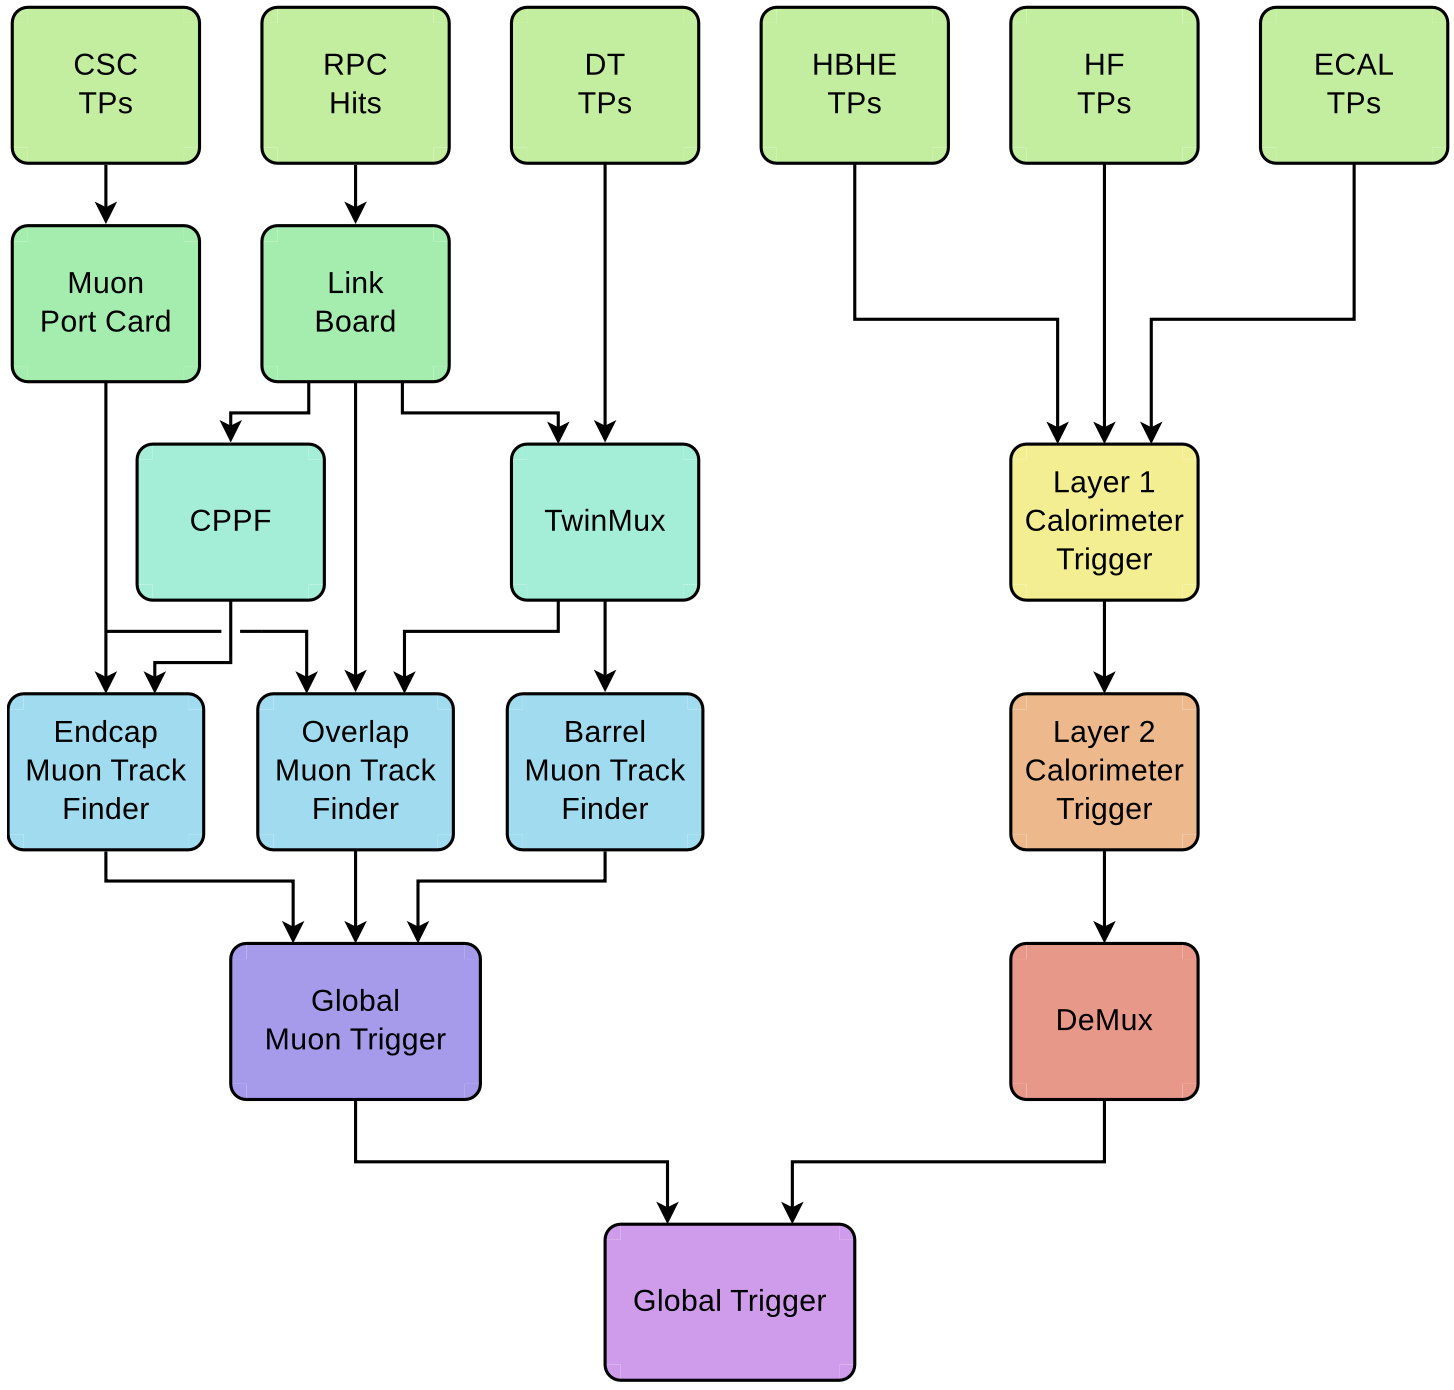
\includegraphics[width=0.75\linewidth]{./Figures/L1TriggerArchitecture.png}
	\caption{A diagram of the L1 Trigger architecture, where the lefthand tree corresponds to the muon triggers and the righthand tree to the calorimeter triggers. Reproduced from \cite{L12020}.}
	\label{fig:L1Architecture}
\end{figure}
\subsection{The L1 e/$\gamma$ Reconstruction}
Since photons and electrons have no associated tracking information, the only way that they can be identified is by their energy signatures \cite{L12020}. The only way to reconstruct e/$\gamma$ objects, then, is to very carefully reconstruct the shape, size, and magnitude of these energy signatures deposited in the TTs of the ECal and HCal. The major tenet of this is called clustering. Firstly, the "seed tower" is defined as the trigger tower that has the highest energy deposition in a local region. Then, contiguous towers are taken where the energy threshold exceeds $E_T = 1$ GeV. These clusters are created dynamically, allowing different signature shapes for later analysis. 

Of course, due to the effects of pileup in the detector elements (as discussed in section (REF?)), care must be taken to consider only those contiguous towers which appear to be part of a genuine e/$\gamma$ signature. There are a few clustering vetos as the L1 level designed to remove signatures that do not appear to origin ate from an e/$\gamma$ candidate: a shape veto is applied to select contiguous clusters that appear to have the correct shape, thereby excluding wider or more irregular pileup showers wherever possible; a fine grain veto bit measures the compactness of the signature in the seed tower and discriminates against hadron-induced showers; an H/E veto measures the ratio of energies deposited in the HCal and ECal, rejecting signatures with higher HCal energy depositions \cite{L12020}.

The next major reconstructed quantity at the L1 trigger is the energy isolation. Essentially, a 6x9 region ($\eta x \phi$) around the main cluster is defined, and the total energy deposited in this region is measured and compared against a chosen threshold for the specific L1 trigger. So, then, a higher isolation energy means that the cluster may not be a clean individual e/$\gamma$ signature and instead could come from a larger hadronic shower or from pileup energy deposition. This isolation energy will be a major component of the HLT and offline reconstructions, as well. The components of the L1 clustering algorithm are shown in figure \ref{fig:L1Clustering}, reproduced from \cite{L12020}.

\begin{figure}[H]
	\centering
	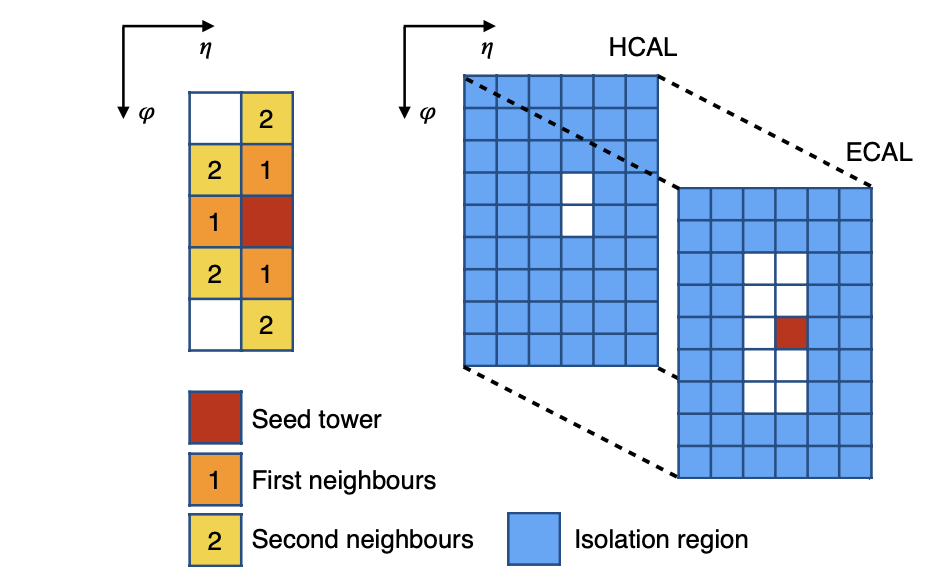
\includegraphics[width=0.75\linewidth]{./Figures/L1Clustering.png}
	\caption{A diagram of an L1 e/$\gamma$ cluster. The central seed tower is shown in red, and the clustered contiguous towers are shown in orange and yellow. The isolation region is shown in blue. Reproduced from \cite{L12020}.}
	\label{fig:L1Clustering}
\end{figure}

The full energy of the cluster, excluding the isolation region, is taken as the "raw energy" of the event and is then compared to various thresholds imposed by differnt L1 triggers. The L1 trigger only has access to this raw energy, the general shape of the energy shower, and the isolation energy. While these quantities will be further refined in later, more sophisticated steps of reconstruction, they still prove powerful enough to reduce the L1 trigger rate to the required value without discarding an unacceptable amount of possibly genuine e/$\gamma$ signatures.
\subsection{The L1 Menu}\label{sec:L1Menu}

The full L1 consists of a suite of many individual triggers combined together, which is termed an L1 menu. While several different menus exist for different physics programs and for testing/calibration, the Global Trigger (GT) menu is the standardized full menu used for normal p-p collisions. This menu consists of the full suite of hadronic, heavy lepton, and e/$\gamma$ triggers. The percentage of the 100kHz rate allowed for each type of trigger in Run 2 is shown in figure \ref{fig:L1Menu}. This information has not been updated for Run 3, but the overall structure of the L1 menu has not changed. Clearly, e/$\gamma$ triggers are a major component of the full L1 menu; combining both single and double e/$\gamma$ triggers gives a total percentage of 31.2\%. 

\begin{figure}[H]
	\centering
	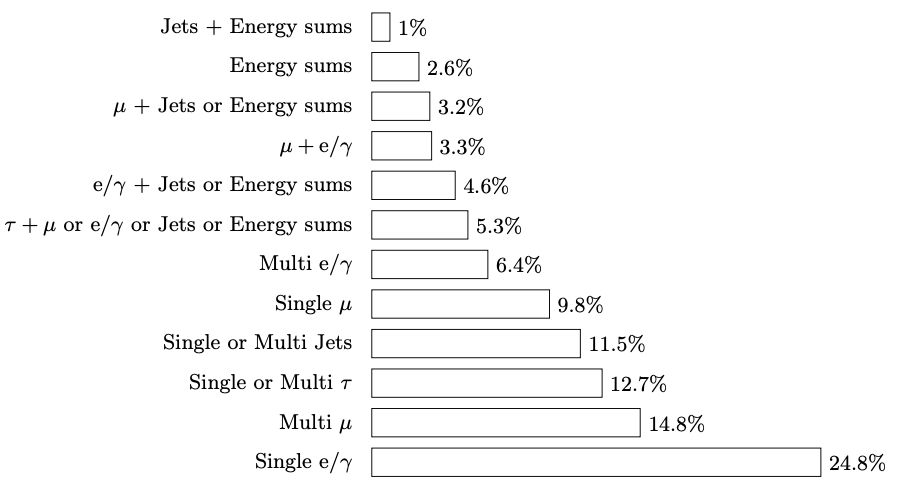
\includegraphics[width=0.75\linewidth]{./Figures/L1MenuPercents.png}
	\caption{A comparison of the percentage of the total rate allowed for each category of trigger. Reproduced from \cite{L12020}.}
	\label{fig:L1Menu}
\end{figure}

Of these classes of triggers, the single and double e/$\gamma$ triggers are the most relevant to the $H \rightarrow \gamma \gamma$.

\section{High Level Trigger} \label{sec:HLT}
The final step of tiggering before data is output for analysis, the HLT aims to reduce the rate from the 110kHz output by the L1 trigger down to a total of just 5kHz \cite{Run2HLT2024}. In contrast to the hardware-based L1 trigger, the HLT is a software-based suite of triggers that runs on a dedicated server of processors called the HLT filter farm. While the L1 trigger menu drastically reduces the overall data rate (by a factor of 400), the HLT is aimed specifically to obtain the best possible events to be provided to analyses. As the last stage before samples are saved and further reconstructed before analysis, the HLT must aim to produce as pure of signal samples as possible. So, then, the signal efficiency of the HLT is of vital importance to every analysis at the CMS. Of course, the details described in this seciton will be of vital importance to an understanding of the development of a BDT-Based HLT for $H \rightarrow \gamma \gamma$. Sections \ref{sec:HLTReco}-\ref{sec:TriggerSoftware} will give a general picture on the reconstruction, rate/timing considerations, and software structure of the HLT as a whole. Section \ref{sec:sHLT}, however, will discuss the details of the current standard HLT for $H \rightarrow \gamma \gamma$. 
\subsection{HLT Event Reconstruction}\label{sec:HLTReco}
Event reconstruction poses both a major challenge and a major strain on the computational resources at the LHC. As a result, reconstruction gets progressively more sophisticated at each stage of event rate reduction \cite{OfflineReco2021}. So, after the primitive reconstruction of the L1 allows that trigger menu to reduce the rate by a factor of approximately 400, the HLT is designed to perform a more thorough reconstruction of the remaining events to help achieve the necessary high signal efficiency. The HLT reconstuction starts with the L1 candidate (termed a L1 seed), and aims to more carefully reconstruct the signature and produce additional quantities derived from the values recorded at L1. 

While the L1 attempts to construct a single cluster as if it came from a single photon or electron, the reality of the detector produces additional complications. In fact, many photons and electrons produced at the interaction vertex will either undergo bremsstrahlung (radiation from the curving of a charged particle) or pair production (the creation of an $e^+/e^-$ pair from an energetic photon) \cite{OfflineReco2021}. As a result, one e/$\gamma$ particle produced from a primary interaction may present as several (often overlapping) signatures in the ECal. Since multiple clusters may overlap, the first step is to determine how much of each energy deposit in a single crystal should be associated with each cluster. A gaussian signature is assumed, centered at the cluster seed. Then, depending on the number of overlapping clusters, an algorithm associates a share of the energy deposited in the crystal with each cluster. At this stage, there is a collection of well-resolved clusters in close proximity.

The most important step of e/$\gamma$ reconstruction is termed superclustering, and it is the process by which neighboring (or overlapping) clusters are associated together into one final supercluster (SC) that contains as much of the signature from the original e/$\gamma$ object as possible \cite{OfflineReco2021}. Superclustering is a two-part algorithm that grows in complexity. Firstly, a "mustache algorithm" uses the basic information from the ECal crystals and the preshower detector to create an initial candidate for a supercluster. Then, a much more complex "refined algorithm" uses information from the trackers to attempt to determine the origin of a specific cluster and ensure that it should be considered part of the supercluster.

The mustache algorithm is so termed because it looks for clusters associated together in a geometric region that resembles a mustache shape. As with the L1 cluster creation, an original seed is chosen as the center of the supercluster. Now, however, the seed is an entire resolved cluster as opposed to a single crystal. Then, two geometric quantities are constructed for each of the surrounding clusters: $\Delta \eta = \eta_{seed-cluster} - \eta_{cluster}$ measures the $\eta$ distance, and $\Delta \phi = \phi_{seed-cluster} - \phi_{cluster}$ measures the $\phi$ distance to the cluster from the central seed. The details of the mustache shape are determined by the algorithm, and depend on the $E_T$ of the seed cluster since charged particles with higher $E_T$ will be bent less by the magnetic field and therefore will have smaller signatures in the ECal. An example of the mustache algorithm is shown in figure \ref{fig:SuperClusterMustache}, where electrons produced with $1 < E^{seed}_T < 10 GeV$ are simulated in the region $1.48 < \eta_{seed} < 1.75$. 

\begin{figure}[H]
	\centering
	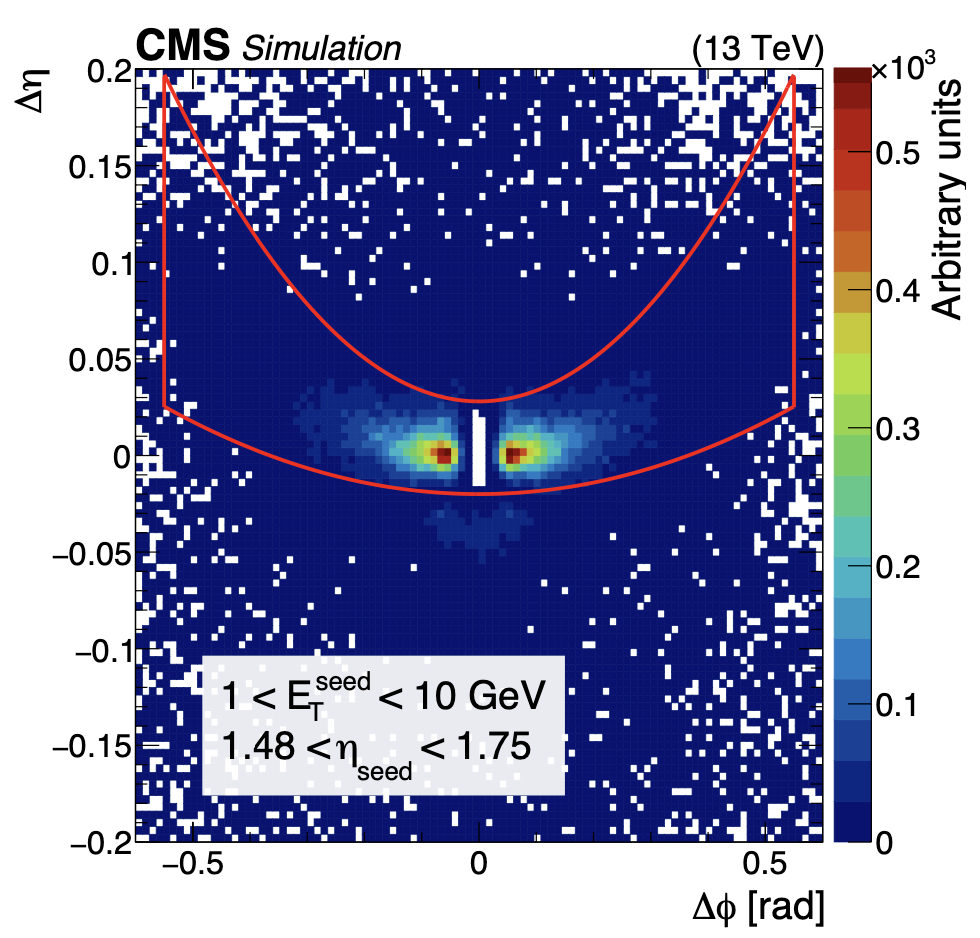
\includegraphics[width=0.75\linewidth]{./Figures/ECalMustache.png}
	\caption{A distribution of the $\Delta \eta$ versus $\Delta \phi$ for the superclustering of simulated electrons. The z-axis represents the number of clusteres matched with the simulation around the seed. The red line represents the set of clusters selected by the mustache algorith. The seed cluster can be seen as the while region in the center of the plot (where both $\Delta \eta$ and $\Delta \phi$ are equal to 0). Reproduced from \cite{OfflineReco2021}.}
	\label{fig:SuperClusterMustache}
\end{figure}

After the mustache algorithm is applied using only the ECal crystals and preshower detector, the much more robust "refined algorithm" applies complex tracking information to further refine the superclustering. The track reconstruction will be described in detail later in section \ref{sec:OfflineReco}, where the differences between the HLT and offline reconstruction will be elucidated. Once the tracks have been constructed, they are used to separate clusters originating from both bremsstrahlung and photon conversion. Bremsstrahlung -- the release of photons due to the bending of an electron track in the magnetic field -- is relatively easy to quantify. Since electrons will have tracks associated with them, the trajectory of the GSF (REF?) track can be measured at each layer of the tracker. Bremsstrahlung photons will be emitted tangentially to the curving electron, so a "bremsstrahlung tangent" can be constructed at each tracker hit to show the direction of such a photon. This tangent can then be linked to a compatible ECal cluster, if one exists.

Photons originating from the primary vertex very often convert to an electron-positron pair. In fact, simulations show that the fraction of photons undergoing conversion can be as high as 60\% where the tracker material is thickest in front of the ECAL \cite{PhotonReco2015}. While the above superclustering is usually able to identify conversion pairs from their resulting shower shape, some events may be recovered by use of the tracking information for the electron-positron pair. In some cases, however, only one of the two legs of the conversion pair may be reconstructed. In order to still reconstruct and preserve these events, a BDT is employed to associate possible conversion tracks to ECal clusters. 

Once a supercluster is constructed and the relevant clusters are added together, various quantities can be reconstructed at the trigger level. Measures of the energy, the shape of the ECal showers, and various isolation measurements can be constructed by using the ECal energy signatures and the tracking information obtained. These variables will be described in more detail in section \ref{sec:OfflineReco}.

\subsection{HLT Trigger Rates and Timing}\label{sec:TriggerRateAndTiming}

In order to appraise the online HLT performance, two major metrics are used: the trigger rate gives a direct measure of how many events the trigger will accept, and the trigger timing measures how long it takes for a decision to be rendered for each event. These two metrics strike at the heart of the major considerations of the HLT; it is vital for storage space that the HLT reduces the total number of saved events, and it is vital for the CPU processing time that each event can be accepted or rejected quickly. 

The limit for the total rate of the HLT in Run 3 is 7kHz \cite{Run3HLTPerformanceConference}. This total rate is composed of 2.5kHz of data processed immediately (prompt data) and 4.5kHz stored for later processing (data parking). Of course, this is the entire rate of the whole HLT menu. As with the L1 trigger menu, there are many types of physics analyses comprising the HLT menu. Figure \ref{fig:HLTRateShares} shows an example of the HLT rate alloted to each physics group. This plot is reproduced from \cite{Run2HLT2024}, and is for Run2 2018 data. While the trigger rate and instantaneous luminosity will be higher for Run 3, the general proportion of rate allotment still holds. Only 12.1\% of the trigger rate is dedicated to Higgs processes, of which there are many. As a result, the overall data rate specifically for $H \rightarrow \gamma \gamma$ analyses will be considerably lower than this. So, any proposed trigger development must be carefully monitored to ensure it does not exceed the rate budgeted to the corresponding analysis.

\begin{figure}[H]
	\centering
	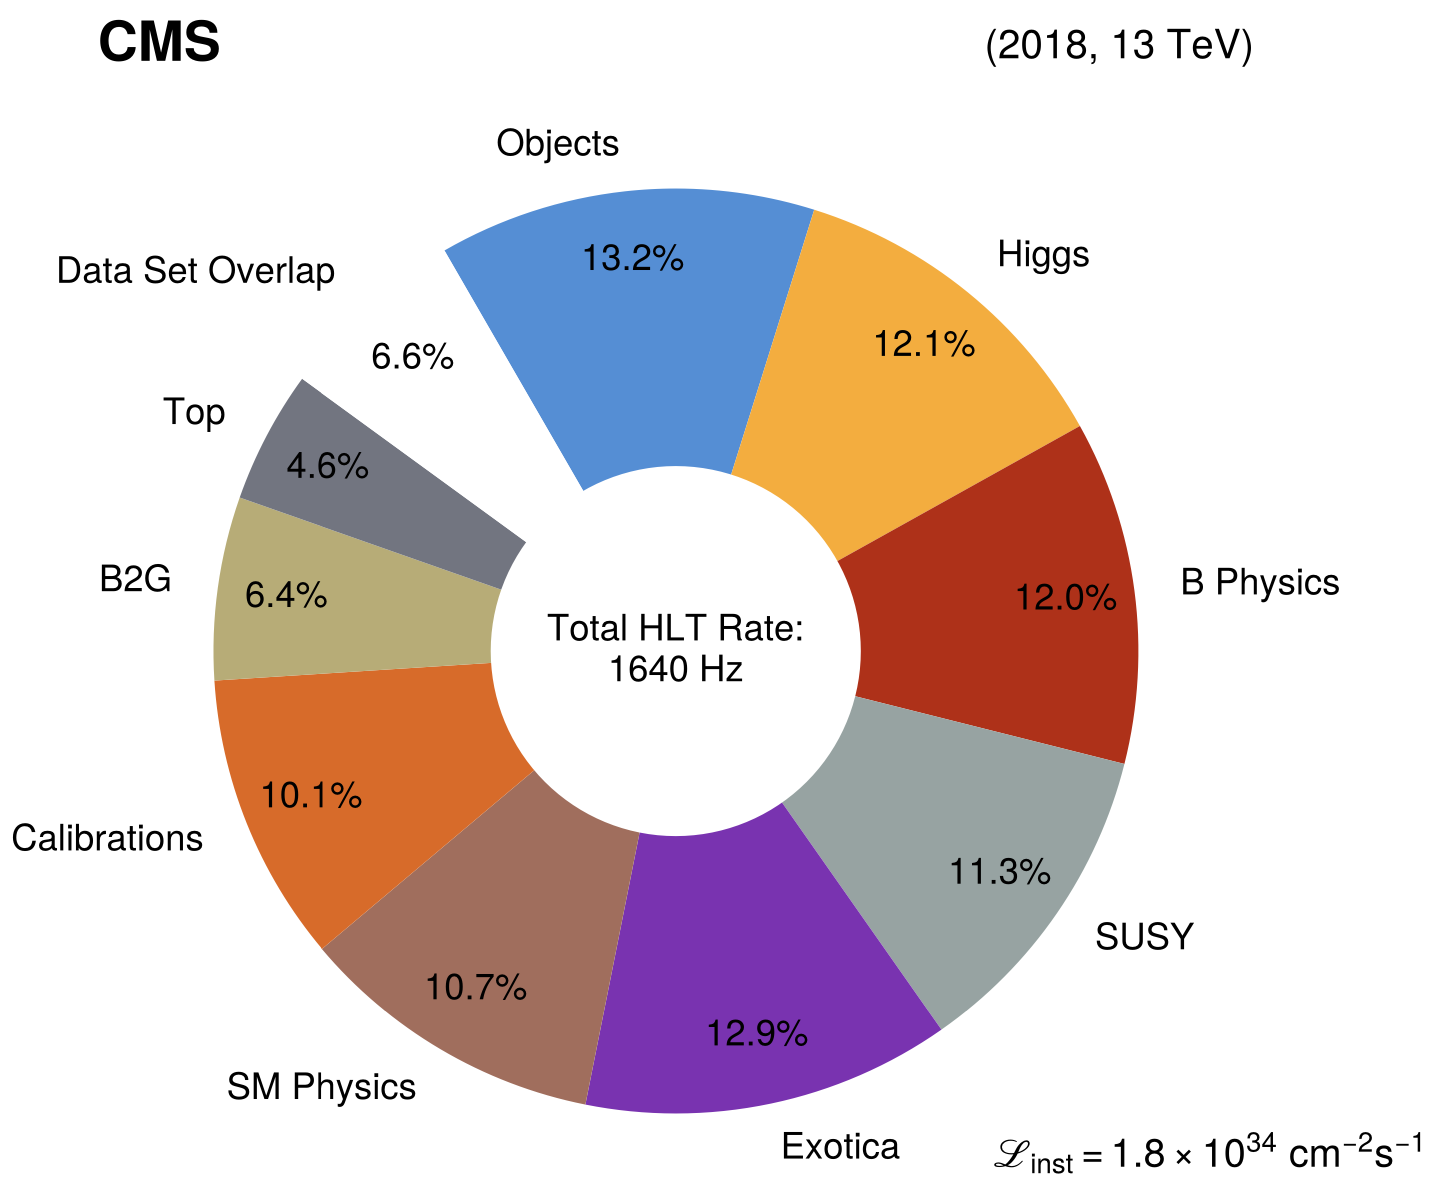
\includegraphics[width=0.75\linewidth]{./Figures/HLTRateConsumptionPieChartRun2.png}
	\caption{A pie chart showing the percentage of the full rate alloted for each physics object group for 2018 data. Note that this example of rate shares operates at a lower instantaneous luminosity and trigger rate than the Run3 data will have. Reproduced from \cite{Run2HLT2024}.}
	\label{fig:HLTRateShares}
\end{figure}

In addition to parking and prompt data streams, "scouting" data streams are taken at a very high rate but with highly compressed information. In early Run 3, these scouting steams reached an average of 26kHz of rate \cite{ParkingAndScouting2024}. These streams only save HLT-level information, and use a simple reconstruction in order to capture rare physics processes at the trigger level using very high rate.

Since many of the events at the trigger level are processed in real time, the amount of time taken per event is a key metric. This timing includes all of the necessary HLT-level reconstruction, as well as the application of whatever cuts and calculations that each individual HLT requires. Since 110kHz of events are passed from the L1 trigger during a standard run period, it is vital that the processing time per event is carefully monitored. As with the trigger rate, any proposed addition to the HLT menu must be verified to have little to no impact on the overall processing time per event. Since much of the time spent processing each event goes towards reconstruction and tracking algorithms, and individual HLT is not liklely to noticably impact the total processing time unless it is egregiously inefficiency.

Moving from Run2 into Run3, the overall data rate has consistently increased year over year. As the storage and processing capabilities have risen, the total allowed rate of the prompt, parking, and scouting datasets has also risen. Additionally, due to improvements to the hardware used to perform the HLT reconstruction (namely, the addition of GPUs in addition to CPUs used in many algorithms), the processing time per event has actually decreased considerably during Run3. Figure \ref{fig:HLTRateAndTiming} , reproduced from (REF? LHCP PAPER), shows both of these effects in detail. At the left, the rates of the various data streams as well as the instantaneous luminosity is shown as a function of the run year. At the right, the total timing is shown for both CPU-only and CPU+GPU processing for the 2022 running year. Of particular interest for this paper is the 2024 run period, as this will be used for the results given in chapter \ref{chapter:Results}.

\begin{figure}[H]
	\centering
	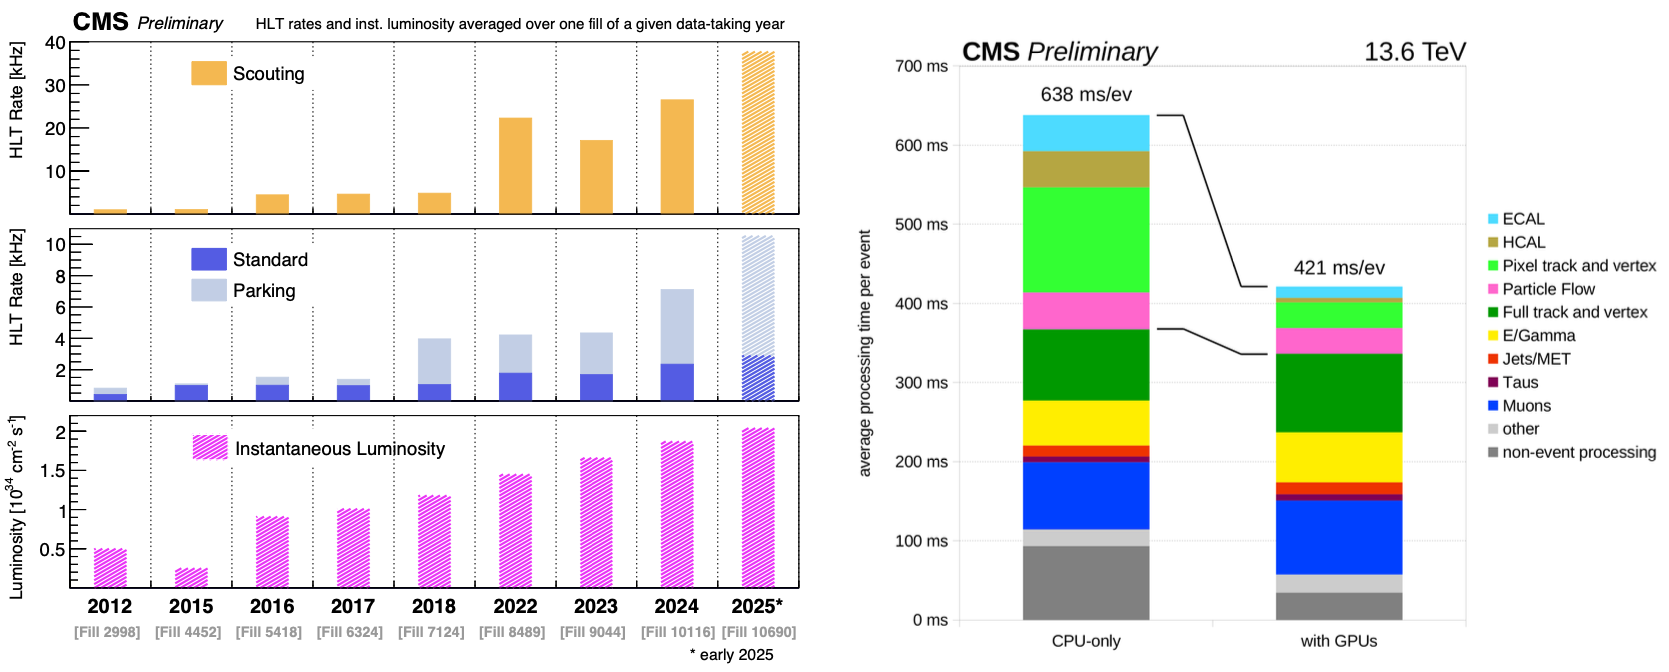
\includegraphics[width=0.99\linewidth]{./Figures/Run3RatesAndTimings.png}
	\caption{On the left, the rates of the scouting dataset (top), prompt (middle, solid), and parking (middle, hatched) data streams are shown. Additionally, the instantaneous luminosity is shown (bottom). To the right, the menu timing is shown with CPU-only and CPU+GPU processing for the 2022 running year. Reproduced from (REF? LHCP PAPER)}
	\label{fig:HLTRateAndTiming}
\end{figure}

\subsection{HLT Software Framework}
The HLT software is built within the CMS Software (CMSSW) framework. Since this is the same software framework used for many future steps of analysis, this provides a relatively standardized set of tools and functions by which the HLT can be constructed. The HLT is of a modular design, where individual modules can be written once and then used by multiple HLTs; many tools, such as the reconstruction of certain quantities or the application of cuts on a specific variable, will be used by a large range of HLTs within the full menu.

There are two major types of HLT modules; EDProducers and EDFilters. An EDProducer module performs a specific step of the reconstruction, starting with a specific prerequisite input and producing a new value as an output. These EDProducers are what allow the input information being passed from the L1 trigger to be reconstructed and combined into more complex variables. For the $H \rightarrow \gamma \gamma$ triggers, EDProducers begin with the e/$\gamma$ candidates constructed at the L1 and produce reconstructed showershape and isolation variables sequentially. These EDProducers vary greatly in there complexity; while some producers perform simple calculations to construct new quantities, many apply complex algorithms and MVA methods to reconstruct objects like tracks. 

After a quantity has been produced by an EDProducer, cuts are often applied to the newly constructed variable using EDFilters. These EDFilters are considerably more simple than EDProducers -- instead of outputting an event, they simply remove candidates that do not pass the selection from the event. An EDFilter can make different cuts on events in the barrel and endcap ECal detectors.

The general structure of the HLT menu is a sequence of EDProducers interspersed with EDFilters. To reduce processing time as much as possible, simple quantities are usually calculated first and cut on, so that the next producer has fewer candidate inputs for which to calculate more complex quantities \cite{OfflineReco2021}. Luckily, a software package called ConfDB exists to more easily handle this construction of an HLT path. Modules (EDProducers and EDFilters) are defined within CMSSW, but then are combined together into sequences and full paths in a graphical interface that allows simple insertion and rearrangenent of modules. This allows preexisting modules to effortlessly be deployed in a new path, minimizing the amount of additional software development necessary to insert a new path into the menu. 

\subsection{Current Standard HLT (sHLT) for $H \rightarrow \gamma \gamma$} \label{sec:sHLT}

Currently, standard $H \rightarrow \gamma \gamma$ analyses rely on a single trigger to accept events for the analysis. This trigger will be termed the sHLT for the remainder of this dissertation. This diphoton trigger is designed to look for a pair of photons that could be constructed to originate from the decay of the Higgs boson. This trigger depends largely on cuts on the showershape, isolation, and kinematics of each photon. After these single photon cuts are applied, possible combinations of the remaining photons are constructed and checked against a final diphoton invariant mass requirement \cite{Run3Hgg2025}. 

Before applying any HLT cuts, the sHLT begins by only considering events passing certain L1 triggers. Specifically, only events passing either the single or double e/$\gamma$ triggers are passed onto the next modules. The single e/$\gamma$ L1 triggers generally have higher $E_T$ requirements on the single photons, whereas the double e/$\gamma$ L1 triggers have looser requirements on the $E_T$ of each photon. The full trigger consists of a combination of two filters. The first "leg" requires a photon candidate to pass a single e/$\gamma$ L1 trigger with an $E_T > 30 GeV$ cut. This L1 seeded leg is the tighter of the two cuts. Then, a second "leg" does not require the tight $E_T > 30 GeV$ L1 seed. Instead, it makes an independent cut on $E_T > 22GeV$. This leg is refered to as the unseeded leg. The final HLT cut requires one photon passing the seeded leg, and another passing the unseeded leg. Each of these filters makes requirements on the showershape and isolation of each photon candidate.

The first showershape cut applied is to the $R_9$. Since this measure of the supercluster shape does a great job excluding non-photon signatures, a hard cut on it allows many QCD-like signatures to be immediately discarded; if a sufficiently large ammount of the super cluster energy is not in the central 9 crystals, the signature is considerably less likely to originate from a photon. The cuts are placed at $R_9 > 0.5$ in the barrel and $R_9 > 0.8$ in the endcap. The values on this cut are different for the two detector regions to account for the different crystal geometries. Next, a hard cut on the H/E is applied. It is expected that hadronic jets will have considerably higher energy deposition in the HCal than the ECal, so large values of H/E are more likely to correspond to non-photon particles. So, then, this cut is placed at $H/E < 0.12$ in the barrel and $H/E < 0.1$ in the endcap. 

The rest of the showershape and isolation cuts depend on the $R_9$ of the photon candidate. If a photon candidate is of high $R_9$ (above 0.85 in the barrel and 0.9 in the endcap), no further cuts are applied. Generally, signatures with such a high $R_9$ are very likely real photon candidates. Below these thresholds, though, additional cuts are applied. Firstly, cuts of $\sigma_{i \eta i \eta} < 0.015$ and $\sigma_{i \eta i \eta} < 0.035$ are applied in the barrel and endcap, respectively. After this, an ECal isolation cut is applied at $\mathcal{I}_{ECal} < 6 GeV$. Taken together, these cuts allow a photon candidate with poor $R_9$ to be preserved if the supercluster is well-isolated with a reasonable shower shape. Finally, to the unseeded leg filter, an additional track isolation cut is applied at $\mathcal{I}_{Track} < 6 GeV$.

Finally, these two filter legs are combined into one final filter. This filter also applies a minimum mass requirement at $M_{\gamma \gamma} > 90 GeV/c^2$. So, then, the final HLT requires that two photons (one with $E_T > 30 GeV$, another with $E_T > 22GeV$) pass the showershape and isolation cuts, and that their combined invariant mass is greater than $90 GeV/c^2$. These showershape and isolation cuts are tabulated in table \ref{tab:sHLTCuts}.
\begin{table}
	\centering
	\caption{Table showing the cuts applied by the standard diphoton HLT for $H \rightarrow \gamma \gamma$. The track isolation cut is only applied to the unseeded second leg.}
	\label{tab:sHLTCuts}
	\begin{tabular}{| c | c | c | c | c | c | c |} 
		\hline
		\textbf{Region} & \textbf{$R_9$} & \textbf{H/E} & \textbf{$\sigma_{i \eta i \eta}$} & \textbf{$\mathcal{I}_{ECal}$} (GeV) & \textbf{$\mathcal{I}_{Track}$} (GeV)\\
		\Xhline{2pt}
		Barrel & [0.5,0.85] & $<$ 0.12 & $>$ 0.015 & $<$ 6.0 & $<$ 6.0\\
		 & $>$ 0.85 & $<$ 0.12 & -- & -- & --\\
		Endcap & [0.5,0.9] & $<$ 0.15 & $>$ 0.035 & $<$ 6.0 & $<$ 6.0\\
		 & $>$ 0.9 & $<$ 0.15 & -- & -- & --\\ 
		\hline
	\end{tabular}
\end{table}

\section{Offline Software} \label{sec:AnalysisSoftware}
After the triggers are processed, refered to as "online" processing, there is still much work to be done. As will be discussed in sections \ref{sec:OfflineReco} and \ref{sec:ParticleFlow}, considerable reconstruction can be done "offline" after the triggers filter events and the partially-reconstructed samples are saved to storage. Whereas the online processing is primarily concerned with reducing the trigger rates as much as possible while preserving maximum signal, the offline processing is aimed at creating final analysis examples with as complete reconstructions and corrections as possible. Additionally, offline processing is aimed at reducing overall file sizes and processing times for future stages in the analysis, as discussed in section \ref{sec:DataTiers}.

\subsection{Offline e/$\gamma$ Reconstruction} \label{sec:OfflineReco}
Many of the details of the offline reconstruction have already been given in section \ref{sec:HLTReco}, as the offline and online reconstruction are designed to be as similar as trigger-level resources will allow. The superclustering performed at the HLT is still performed offline, as this is a relatively lightweight algorithm that provides great power to the HLT. The major difference for e/$\gamma$ objects between the two levels of reconstruction, however, lies in the tracking information. Since tracks must be constructed by complex algorithms combining many tracker hits, this process is largely pared back at the trigger level. 

Both the HLT and offline electron track reconstruction are based on a Gaussian Sum Filter (GSF) \cite{GSFTracking}. Since this process is very CPU-intensive, it is not done for all possible tracker hits. Instead, electron tracks begin with a hit pattern that might correspond to an electron track, called a "seed". These seeds take two forms. ECal-driven seeds start from a mustache SC satisfying specific criteria, then finds tracker hits that may be associated with this seed. All HLT-level tracks are ECal driven, which is one of the major ways that the processing time is kept within the strict limits of that level. Tracker-driven seeding looks at all possible generic tracks and applies algorithmic selections to identify those possibly originating from an electron.

ECal-driven tracker seeds first select a mustache SC which satisfies $E_{SC,T} > 4 GeV$ and $H/E_{SC} < 0.15$, where $E_{SC}$ is the total supercluster energy and H is the energy of all HCal towers within $\Delta R = \sqrt{(\Delta \eta)^2 + (\Delta \phi)^2} = 0.15$ of the center of the SC position \cite{OfflineReco2021}. Then, triplets and doublets of inner pixel tracker hits are combined, and the relative positions of these possible tracks in $\phi$ and z are compared to the ECal SC. The track is then extrapolated back towards the collision vertex using the SC location the seed energy, and the strength of the magnetic field in the region through which the track moves. If the first two hits of a tracker seed are matched to this predicted trajectory from the SC, then the tracker seed is chosen to seed a GSF track. This ECal-driven track seeding is $>$ 95\% efficient for tracks with $E_T > 10GeV$ \cite{OfflineReco2021}.

The tracker-driven approach iterates over all possible generic tracks coming from the interaction vertex, and is therefore much less CPU-efficient. An iterative algorithm called the Kalman Filter (KF) is used to reconstruct every possible track. A combination of cut-based selection OR a BDT-based selection criteria are applied to each track, and if it is found to be compatible with a ECal cluster it is used as a seed for a GSF track. Given the complexity of this seeding procedure, it becomes clear why this tracking algorithm is not applied in the HLT reconstruction.

Once a collection of ECal- and tracker-driven tracking seeds is created, the actual electron tracks can be fully reconstructed. Now, the KF algorithm is used iteratively to build the track from each tracker hit beginning from the first tracker layer and moving outward. Each step along the way, the energy loss of the electron due to collisions with the tracker material is modeled. If the next tracker layer has multiple possibly associated hits, up to 5 track trajectories can be built using a $\chi^2$ fit. Conversely, in the case where a single hit may belong to multiple possible tracks, the hit is associated with the track with either the least number of missing hits or the lowest $\chi^2$ value. After the KF algorithm reconstructs a track candidate, a GSF fit is used to estimate its parameters at each tracker layer.

Once a GSF track candidate is obtained, it must be associated conclusively with an ECal cluster to form a final electron candidate. This process is termed track-cluster association \cite{OfflineReco2021}. This association is performed using a complex BDT. The BDT is trained on track kinematic and quality variables, SC showershape variables, and track-cluster matching variables. Since this BDT is so complex, it is immediately clear why the number of GSF candidates must be properly reduced before full track reconstruction. The track-cluster association is handled differently for tracker-driven and ECal-driven seeds. For track-driven seeds, a cut on this BDT is used to determine if a track and cluster are associated. For ECal-driven seeds, either the same BDT requirement or cuts of $\lvert \Delta \eta \rvert < 0.02$ and $\lvert \Delta \phi \rvert < 0.15$ are applied, where the differences are between the actual SC location and the location of closest approach to the SC of the extrapolated track. 

\subsection{Particle Flow Reconstruction}\label{sec:ParticleFlow}
Another major difference of the offline reconstruction is the existence of the particle-flow (PF) algorithm. At its most basic level, the PF algorithm seeks to combine all possible particle information into one cohesive algorithm \cite{ParticleFlow}. PF is able to establish the 4-momenta of each particle in an event, and identify it as a hadron, photon, electron, or muon. This final categorization allows additional quantities to be calculated, and is the full particle reconstruction used for analysis \cite{OfflineReco2021}. For e/$\gamma$ objects, the primary elements to link together are tracks and ECal clusters. ECal clusters have been discussed in detail in section \ref{sec:HLTReco}. Tracking has been discussed in section \ref{sec:OfflineReco}. 

A major piece of information added to the event record at the offline software level is the vertexing information. By tracing a track backwards towards the interaction region, a specific location of collision, called the primary vertex, can be constructed. Reconstructing this vertex is a key part of the full particle flow algorithm. This vertex is constructed using the full tracking information for electrons, and is therefore dependent on the offline track reconstruction discussed above \cite{PhotonReco2015}. 

In order to fully reconstruct an e/$\gamma$ object, the ECal clusters, full tracking information, and vertexing information must be combined into the PF algorithm. The first step of PF is called the link algorithm designed to link together signatures from the different subdetectors into a single signature. The link algorithm works pairwise, considering possible pairs of signatures in nearby detector elements that may be worth associating. Of course, given the dozens to hundreds of possible detector signatures, this could quickly become overly CPU-intensive. So, the link algorithm only considers elements nearby eachother in the ($\eta$,$\phi$) plane \cite{ParticleFlow}. Several possible links between signatures will be discussed in the next paragraphs. Once links are established, PF blocks are constructed that consist of multiple linked elements fed into the PF algorithm.

% As with the track-cluster association discussed above, the PF algorithm attempts to link a fully reconstructed track with an ECal cluster. The full track is extrapolated from the final tracker hit obtained, and a proposed final cluster hit is defined within the ECal. If there is an ECal cluster within a defined distance in ($\eta$,$\phi$) for the barrel or (x,y) in the endcap, the track and cluster are considered linked. A distance between the extrapolated endpoint and the actual cluster his is created, and the track with the smallest distance is linked to the cluster \cite{OfflineReco2021}.

(IS TRACK-CLUSTER ASSOCIATION THE SAME AS PF LINK ALGORITHM? I Think so). In addition to the track-cluster associated discussed in section \ref{sec:OfflineReco}, the PF algorithm must link other elements together. Cluster-cluster linking associates hits within the ECAL with hits in the HCAL. As with the track-cluster linking, a distance is determined in the ($\eta$,$\phi$) plane in the barrel and the (x,y) plane in the endcaps. If multiple links are possible, the algorithm simply chooses the linked elements with the smallest separation distance. Links are made between tracks if a common secondary vertex can be found between two tracks. These displaced vertices come from interactions of a primary particle with the material, which then can produce two or more associated particles some distance from the prinary vertex. If a track between the primary and secondary vertex, corresponding to the primary particle, can be reconstructed, then that track is linked with the tracks originating from the secondary vertex. Finally, linking between inner tracker tracks and the muon detector can be linked, though that is not relevant for this analysis.

The final PF reconstruction follows a standardized progression \cite{ParticleFlow}. Firstly, possible muons are reconstructed. Since muons will produce a clear signature in the muon detectors where few other particles will be found, this reconstruction is used to remove associated tracker and calorimeter hits from the PF block. Then, the electron reconstruction is performed, aiming to differentiate between electrons and well-isolated photons. Again, tracks and clusters identified by these reconstructions as part of an electron or photon are removed from the PF block. Finally, hadron reconstruction is handled with the remaining signatures. Of course, due to the focus of this paper on $H \rightarrow \gamma \gamma$, only the details of the e/$\gamma$ reconstruction are of particular interest.

As already mentioned, electrons very regularly emit bremsstrahlung photons, and photons very regularly undergo $e^+ e^-$ conversion due to the material in the detector. The $e^+ e^-$ from converted primary photons even undergo bremsstrahlung themselves, often. As a result, even at the PF level, electrons and photons are very hard to reconstruct separately. The primary differentiator used by the PF algorithm is the association with a GSF track \cite{ParticleFlow}. If a GSF track can be linked to an ECAL cluster without 3 or more additional tracks involved, than the particle is seeded as an electron candidate. If a ECAL cluster with $E_T > 10GeV$ cannot be linked with a GSF track, the particle is seeded as a photon candidate.

Then, the HCAL energy deposition within a distance of 0.15 in ($\eta$,$\phi$) must be less than 10\% of the ECAL supercluster energy for both photon and electron candidates. This helps make sure that the signature is not a misidentified hadronic jet, which would deposit much of its energy in the HCAL. After this requirement, ECAL clusters and GSF tracks must be associated with the candidates. Any ECAL cluster that can be associated with the supercluster or with the tangent of a GSF track (thereby being a bremsstrahlung photon) is automatically added to the candidate. Once the ECAL clusters from the PF block are selected, any track linked to these clusters is accepted as long as the energy and momentum deposited in the HCAL is consistent with the electron hypothesis.

The final identification of electron candidates is much more intensive than that for photons. A complex BDT is used to determine whether a chosen electron candidate can be positively identified as an electron. This BDT uses input variables related to the GSF tracks, the KF $\chi^2$, and the total number of hits \cite{ParticleFlow}. Photon candidates are then checked on two metrics. First, the photon must be well-isolated from other tracks and clusters in the event. Secondly, the showershape and H/E values must be consistent with a photon shower. 

\subsection{Data Formats at Different Reconstruction Levels}\label{sec:DataTiers}
Any given sample of either data or monte carlo generated by the CMS experiment pass through a full data flow with subsequent steps of reconstruction and size reduction \cite{MiniAOD}. Data begins its life in the RAW format, which contains only the information available to the HLT as discussed in section \ref{sec:HLTReco}. Then, the RECO format is created, which adds all of the online reconstruction information from the HLT reconstruction to the RAW format. This RECO format serves as the input to the final offline reconstruction described in section \ref{sec:OfflineReco}. Whereas the RAW data format consists of about 1MB of disk space per event, the RECO format takes about 2-3x as much space \cite{NanoAOD}. The trigger developments that will be discussed later in chapter \ref{chapter:HLT} are performed on the RAW data format.

The next three stages of data formats contain essentially the same information, but aim to progressively reduce the storage size of the sample. This is achieved in two ways: the total number of events stored in the data can be reduced by a process called "skimming"; the size of each event can be reduced by eliminating event content. The skimming process is generally handled by the trigger system. After the RECO format, event information is summarized and reduced in multiple steps in order to reduce the size of each individual event. 

The first data format constructed by CMS was the Analysis Object Data (AOD) tier, first implemented in Run 1 of the LHC. The AOD format reduces the storage size per event by about 85\% compared to the RECO form at \cite{NanoAOD}. This process takes a huge amount of processing time, so it is generally not rerun often. In fact, the AOD processing typically runs immediately after the data is collected or the MC is generated, and is only rerun every few years as updates to the offline reconstruction or the AOD format are implemented. This AOD format was the primary centrally-produced data format throughout Run 1.

A major design philosophy difference between the RECO (online) and AOD (offline) data formats is the structuring of data into physics objects. After the PF algorithm is applied to an event, it can be structured according to high-level physics objects such as hadronic jets, isolated photons and electrons, and muons \cite{ParticleFlow}. So, then, every event has a collection of possible physics objects for each subsequent data tier. Additionally, very simplified individual particle candidates containing mostly kinematic information determined by the PF algorithm can be saved. This is a fantastic step towards making the data as analysis-friendly as possible; a $H \rightarrow \gamma \gamma$ analysis, for example, can simply concern itself with the collection of photon physics objects and disregard information on jets, muons, and other leptons. So, then, the AOD formats help not only to reduce the required storage space, but additionally reduce the burden on each analysis group by making the data easier to traverse.  

For Run 2, with the proliferation of data and MC produced, an updated centrally-produced format was needed to reduce the storage size of samples. This led to the introduction of the MINIAOD format \cite{MiniAOD}. This format aimed to reduce the per-event storage size by an additional factor of 10 relative to the AOD format. While some event information is lost at this data tier, 95\% of physics analyses in Run 2 are able to use the format without issues. The remaining 5\% can run private production of custom data formats directly from the AOD. An additional benefit of this process is that the MINIAOD processing can be rerun multiple times a year, allowing for more frequent updates to reconstruction and callibraton \cite{NanoAOD}. The MINIAOD format contains both high-level physics objects (leptons, photons, and jets). It also contains the very basic particle candidates identified by PF, which contain basic kinematic information.

For Run 3, the NANOAOD format was introduced to provide an even further reduced storage size. This format is able to reduce the per-event storage to about 1-2kB per event, which is a reduction of a factor of over 1000 compared to the RECO format \cite{NanoAOD}. The NANOAOD is very regularly changing and being updated as different analysis groups' needs change; processing the NANOAOD from the MINIAOD is a very fast process that can be run without undue strain on computation resources. There is a reduction in the per-event information saved, so in reality about 70\% of analyses in Run3 will be able to solely use the NANOAOD format. Other groups are still able to access the MINIAOD format for their specific needs.

The NANOAOD format is the data format used for the final results of this paper shown in chapter \ref{chapter:Results}. The general structure of this data tier is very easy to use and understand. Whereas the MINIAOD format is composed of physics objects that must be accessed with specific CMS software, the NANOAOD format is structured as "trees" that can be directly accessed using standardized ROOT software \cite{NanoAOD}. Each tree has a collection of "branches" which correpond to specific physics observables. Within each branch, there is an array of all of the values associated with a particular event. So, this event-based architecture allows event information to quickly be access and traversed, leading to much improved ease in analysis compared to previous data formats.  

In order to achieve this massive reduction in event size, much of the low-level detector information such as tracks and clusters are dropped from the event. Furthermore, many of the inputs used for identification algorithms are dropped, with the NANOAOD opting to instead keep only the outputs of the identifications \cite{NanoAOD}. Additionally, many of the high-level physics quantities saved are redundant with the lower-level information used to derive them. So, many of the lower-level information bits that could later be rederived if necessary are omitted from the event collections. If, for some reason or another, it is later deemed necessary to restore any of the information omitted from the NANOAOD, a new version can be updated to include it rapidly. 

\chapter{Boosted Decision Trees and XGBoost} \label{chapter:BDTs}
The newly-proposed trigger and complementary offline selection -- discussed in chapters \ref{chapter:HLT} and \ref{chapter:OfflineSelection}, respectively -- is based on a machine learning construct called a Boosted Decision Tree (BDT). This ML method provides a robust and relatively simple algorithm for binary classification problems, which works well both with the HLT and with subsequent offline classification and event selection. The theoretical details and structure of BDTs is described in section \ref{sec:BDTBasics}. The software package XGBoost (short for eXtreme Gradient Boosting) will be used for both the creation and evaluation of the BDTs employed at the trigger and offline analysis levels. This software is described in more detail in section \ref{sec:XGBoost}.
\section{Gradient Descent Boosting} \label{sec:BDTBasics}
The original description of boosted decision trees and gradient descent boosting is described in "Greedy Function Approximation: A Gradient Boosting Machine" by Jerome H. Friedman \cite{BDTPaper}. The following section is largely based on this seminal paper, with emphasis placed on the facets of the technique most relevant to this paper. 

At its core, a binary classification problem is a function estimation problem; a function must be constructed that maps some input values onto a single output score. The general parlance is to label the input variables for a single event as $\vec{x} = \{x_1, x_2, ... x_n\}$, where n is the total number of selected input values. The output, however, is a single score, usually labeled $y$. There exists some theoretical function, $F^{*}(\vec{x})$ that directly maps $\vec{x}$ onto $y$. This function cannot be known exactly for problems of moderate complexity, so an estimate of this function, $\hat{F}(\vec{x})$, is the goal of the gradient boosting process. 

To quantify how closely the approximation $\hat{F}(\vec{x})$ follows the true $F^{*}(\vec{x})$, some loss function must be defined. There are many forms of loss function, as will be described in section \ref{sec:Objective Function}. The loss function is termed $L(y,F(\vec{x}))$, meaning that  it quantifies how closely the approximate points, $F(\vec{x})$ , follow the true classification values of the events, $y$. Given these definitions, the goal of the BDT algorithm can be written as given by Friedman \cite{BDTPaper}.
\begin{equation}\label{eqn:FriedmanOverallFunction}
    F^{*} = \underset{F}{min} \: E_{y,\vec{x}}[L(y,F(\vec{x}))]
\end{equation}

\section{The Objective Function} \label{sec:Objective Function}
\section{XGBoost Software} \label{sec:XGBoost}


\chapter{Development of an MVA-Based High Level Trigger}\label{chapter:HLT}
\section{Limitations and Benefits of Current $H \rightarrow \gamma \gamma$ Trigger} 
As discussed in section \ref{sec:HLT}, the current $H \rightarrow \gamma \gamma$ HLT uses hard cuts on kinematic, isolation, and showershape variables to select events. While cuts on some of these variables -- such as $R_{9}$ and H/E -- serve to remove low quality photon candidates, others reduce the phase space of the trigger while not necessarily increasing the quality of the analysis. Principally, the current HLT makes rather tight cuts on the $p_{T}$ of the two photon candidates. These cuts significantly reduce the trigger rate, as many background processes produce showers with low $p_{T}$. Many signal events, however, have at least one candidate with low $p_{T}$. It will be shown in section \ref{sec:cutChoices} that these $p_{T}$ cuts significantly decrease the acceptance of simulated Monte Carlo signal events. Since many future analyses will be searching for either very rare processes or physics beyond our current understanding of the standard model, constraining the phase space of available information may affect the collaboration's ability to probe novel processes. 

The relative simplicity of the standard HLT, however, provides multiple benefits. Firstly, the numerical cuts can be closely examined and understood very easily. Though the cuts have been relatively stable in time, they may adjusted and reexamined with relative ease. The effects of cuts on individual variables can be quantified, which allows maximum transparency into how a decision is made on an event-by-event basis. Secondly, a decision for each event can be made very rapidly. As discussed in section \ref{sec:timing}, minimizing computation time for each event is vital given the huge number of triggers deployed at the trigger farm. Since all of the quantities used by the current HLT are already being saved for each event, there is very little additional computation needed to arrive at a triggering decision. Any proposed changes to the $H\rightarrow\gamma\gamma$ trigger must have minimal impact on decision speed given the stringent restrictions on computation time.

\section{Development of a Boosted Decision Tree for Photon Candidate Classification}
The HLT is a binary classification problem, where the two classes are signal events to keep and background events to discard. While the HLT is a per-event selection, $H \rightarrow \gamma\gamma$ events contain two photon candidates. As described in \ref{sec:HLT}, the current HLT first makes requirements on individual photons, then applies a final filter that considers both photons together. Our MVA-HLT uses a similar philosphy; a binary classifier can be used to calculate an identification score for each photon, then combined cuts can be made on these scores for two photon candidates. The process of creating the MVA-HLT, then, is twofold. Firstly, the single photon binary classifier must be constructed such that signal-like photon candidates are given a high score and background-like photon candidates are given a low score. Secondly, cuts on both photon candidate scores must be selected such that the signal efficiency is maximized while the data rate is minimized.
\subsection{XGBoost-Based BDT Software}\label{sec:HLTXGBInfo}
XGBoost is a commonly-used software package throughout CMS, as it excells at binary classification problems. Specifically, Boosted Decision Trees (BDTs) are used commonly in CMS software (REF?). BDTs provide a good balance between model complexity and transparency. By tuning a relatively small number of model hyperparameters, as discussed in section \ref{sec:hyperparameters}, model complexity can be controlled and understood. For the development of this BDT, the python version of XGBoost was used, though the final implementation of the model must be done in the C-based CMSSW (as discussed in section \ref{sec:HLTImplementation}). 

\subsection{Signal and Background Samples for Classification}
The first -- and perhaps most important -- step in creating a binary classifier is selecting samples on which to train the BDT. It is important that the signal sample chosen accurately represents the type of events that should be kept at the HLT, while the background sample must encompass all possible source of background events. 
\subsubsection{Signal Samples}\label{sec:HLTMCSamples}
As discussed in (REF?), Monte Carlo simulations exist for various physics processes that contribute to $H \rightarrow \gamma\gamma$. While there are several common production modes for the Higgs boson (as discussed in section (REF?)), gluon fusion Higgs production (ggH) has the largest production cross section. In addition to the large cross section, ggH production has fewer assiciated productions when compared to VBF or ttH Higgs production. For these reasons, ggH signal MC provides a clean signal that maximizes the photon discrimination ability of a BDT. 

In order to validated the performance of the model, the acceptance of these signal MC events must be quantified. As a result, half of the sample is used for training, while the other half is reserved for later validation. Events are split by event number into two separate categories: even event nubers are used for the training sample, and odd event numbers will be used for the validaiton of the model performance. 
\subsubsection{Background Samples}\label{sec:HLTDataSamples}
At the trigger level, background simulation poses a major challenge. Background events for $H \rightarrow \gamma\gamma$ fall into three major categories: events containing two photons diphoton, events containing a photon and a jet, and events containing two jets. While it is possible to simulate these background sources, the simulation -- especially of the jet-jet events -- is challenging and therefore may not perfectly allign with the real data. The most obvious resolution to this issue is to simply treat the data sample as background. While, of course, the goal of the trigger is to preserve signal signatures from the data, it has been shown in chapter \ref{chater:Theory} that the overall expected count of signal events in this data sample is relatively low. As long as a clean signal sample is provided to the BDT, the incredibly small percentage of possible $H \rightarrow \gamma\gamma$ events in the data should not appreciably mar the model's ability to differentiate signal and background photon candidates. As with the signal MC, even event numbers are used for the training, while odd event numbers are reserved for later validation of model performance.
\subsection{Determination of Input Variables}
After signal and background samples are selected, input variables for the BDT must be chosen such that signal and background events can be separated. The most obvious starting place for this is by analogy to the current HLT; since cuts on the kinematic, isolation, and showershape variables have been successfully used in the preexisting trigger, a BDT should be able to use these variables to even greater effect. Below, in table \ref{tab:HLTInputVars}, the chosen input variables are listed along with their definitions.
\begin{table}
	\centering
	\caption{Table of input variable names, and a short description of each.}
	\label{tab:HLTInputVars}
	\begin{tabular}{ | c | c | } 
		\hline
		\textbf{Variable Name} & \textbf{Description} \\
		\Xhline{2pt}
	  	Raw Energy & The total energy deposited in the 5x5 supercluster  \\ 
		\hline
		$R_{9}$ & \makecell{The proportion of the energy contained in the central 3x3 crystals \\ relative to the raw energy}  \\ 
		\hline
		$\sigma_{i \eta i \eta}$ & The covariance in terms of crystal spacing ($i_{\eta}$)\\ 
		\hline
		$\eta_{SC}$ & The eta coordinate of the center of the supercluster  \\ 
		\hline
		$\eta$ Width &  The supercluster width in $\eta$ \\ 
		\hline
		$\phi$ Width &  The supercluster width in $\phi$ \\ 
		\hline
		H/E & \makecell{The ratio of the total supercluster energy measured in the HCal \\ to that measured in the ECal}  \\ 
		\hline
		ECalPFIso & The isolation energy of the particle deposited in the ECal\\ 
		\hline
	\end{tabular}
\end{table}

The chosen variables are largely showershape and isolation variables, as these can be used to differentiate a legitimate photon signature from a jet shower. A major goal of the BDT is to increase kinematic coverage; relying primarily on showershape variables ensures that the selection is not biased towards a specific kinematic region. Below are plots of the above input variables, where the signal MC is shown in dark (barrel) and light (endcap) blue, while the data is shown in red (barrel) and pink (endcap). These distributions are self-normalized, so the y-axis value corresponds to the ratio of events in that bin versus the entire distribution.

\begin{figure}[H]
	\begin{subfigure}{0.50\linewidth}
		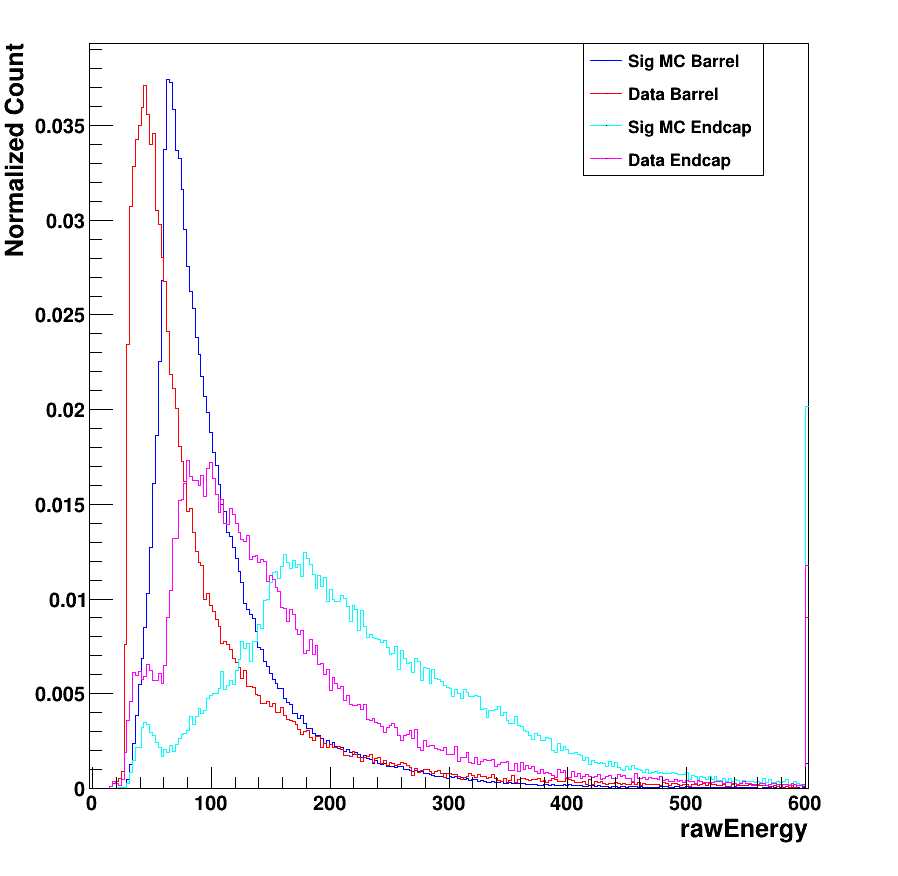
\includegraphics[width=\linewidth]{./Figures/Trigger Training Plots/0713_2026_NormalizedTrainingVars/rawEnergy.png}
		\caption{Raw Energy}
		\label{HLTVars:RawE}
	\end{subfigure}\hfill
	\begin{subfigure}{0.50\linewidth}
		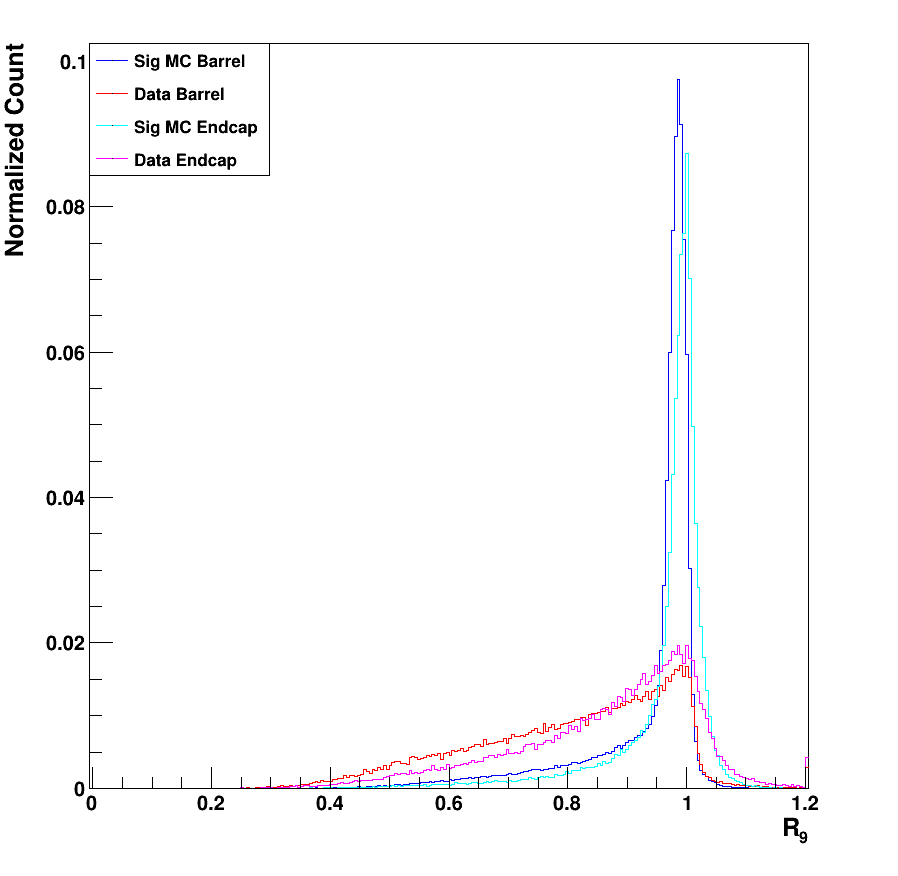
\includegraphics[width=\linewidth]{./Figures/Trigger Training Plots/0713_2026_NormalizedTrainingVars/r9.png}
		\caption{$R_9$}
		\label{HLTVars:r9}
	\end{subfigure}
	\caption{Plots of raw supercluster energy and $R_9$. The signal MC is shown in dark blue for the barrel and light blue for the endcap, whereas the data (background) is shown in red for the barrel and pink for the endcap.}
	\label{fig:HLTVars1}
\end{figure}

The raw supercluster energy gives a measure of the total energy deposited in the ECal supercluster. In figure \ref{HLTVars:RawE}, it can be seen that the signal MC has a slightly higher center than the background in the barrel. This difference is more pronounced in the endcap, however, where the signal MC has a considerably higher average raw energy. The separation in these two detector regions is not major, however. The $R_9$, on the other hand, proveds to be a very well-separated training variable. For both the barrel and endecap, the signal distributions seen in \ref{HLTVars:r9} are very well-peaked near 1. This means that most of the signal MC events have a very large percent of their energy deposited in the central 3x3 crystals of the supercluster. This is often the case for real photons, as their geometric extent is smaller than that of jets. The data, however, is a much broader distribution. While it peaks near 1, there are still many photon candidates with $R_9$ approaching lower values. Since QCD jets tend to have a larger geometric extent, this is expected. As a result, this is a very strong discrimination variable for the binary classifier BDT.

\begin{figure}[H]
	\begin{subfigure}{0.50\linewidth}
		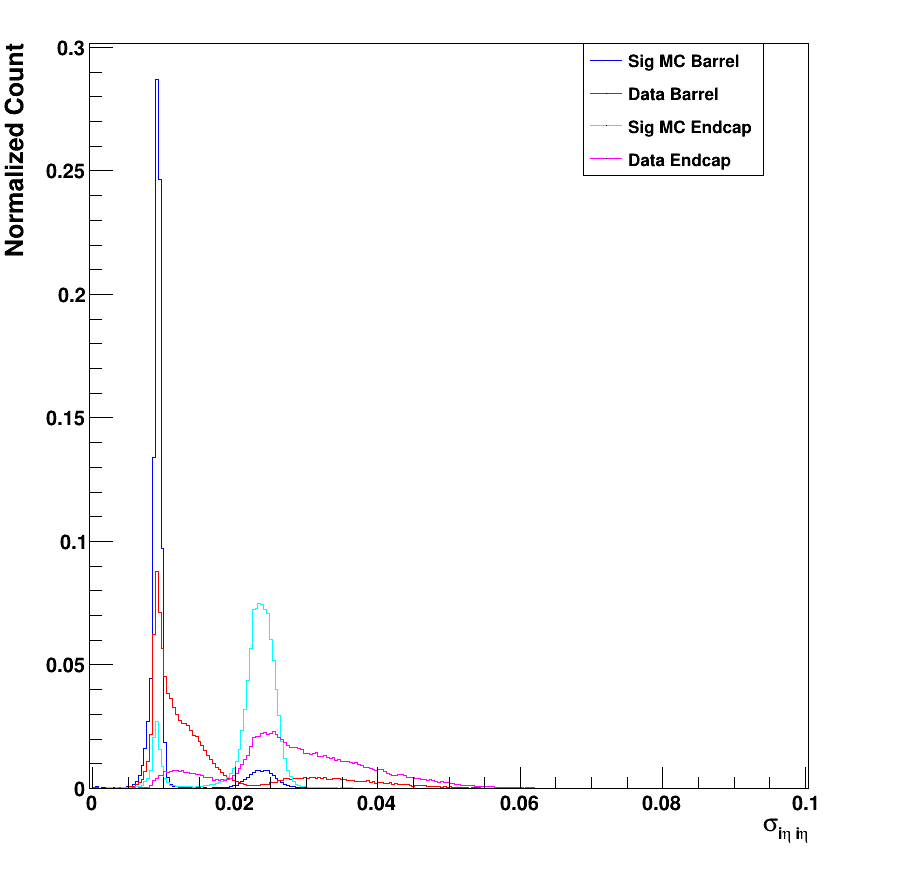
\includegraphics[width=\linewidth]{./Figures/Trigger Training Plots/0713_2026_NormalizedTrainingVars/siEtaiEta.png}
		\caption{$\sigma_{i \eta i \eta}$}
		\label{HLTVars:Sieie}
	\end{subfigure}\hfill
	\begin{subfigure}{0.50\linewidth}
		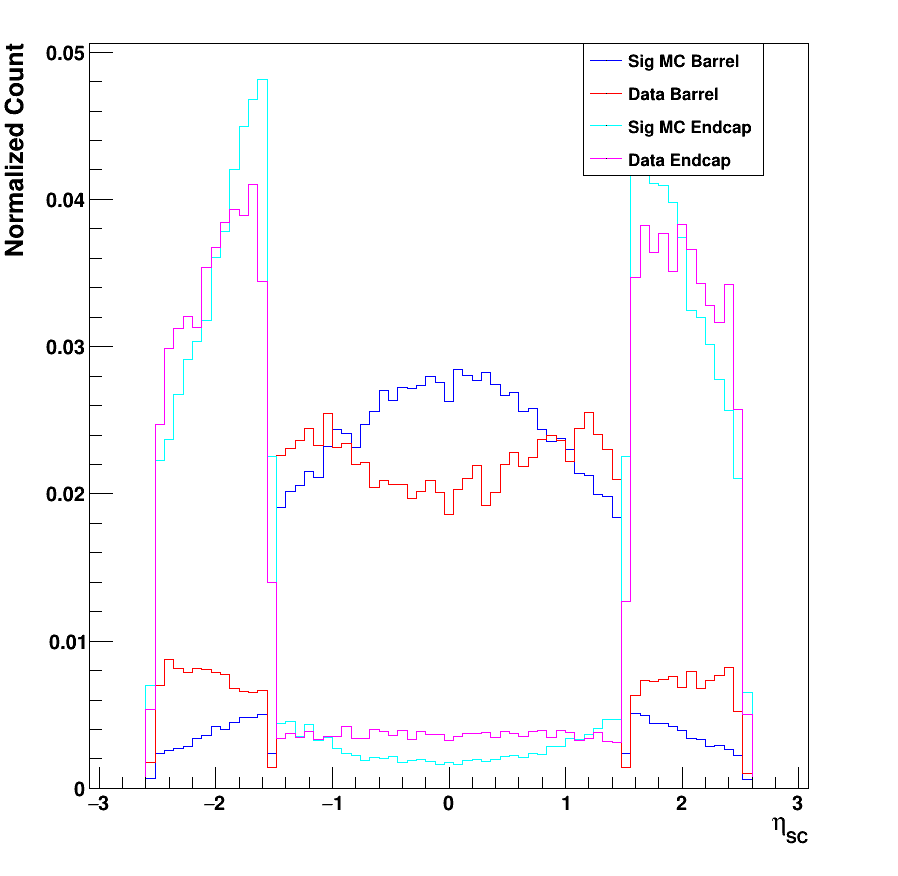
\includegraphics[width=\linewidth]{./Figures/Trigger Training Plots/0713_2026_NormalizedTrainingVars/eta.png}
		\caption{$\eta_{SC}$}
		\label{HLTVars:Eta}
	\end{subfigure}
	\caption{Plots of the $\sigma_{i \eta i \eta}$ and $\eta_{SC}$. The signal MC is shown in dark blue for the barrel and light blue for the endcap, whereas the data (background) is shown in red for the barrel and pink for the endcap.}
	\label{fig:HLTVars2}
\end{figure}

The $\sigma_{i \eta i \eta}$ is another showershape variable that has powerful discrimination abilities. As can be seen in figure \ref{HLTVars:Sieie}, the barrel and endcap are rather well-separated for both the MC and data. This is due to the difference in crystal positioning in the two detector regions; since the endcap crystals are larger with larger spacing as described in section \ref{sec:ECal}, the $\sigma$ in terms of the crystal spacing tends to be larger. Additionally, it is immediately obvious that the photon candidates from the signal MC are much more sharply peaked in both the barrel and endcap relative to the data events. Given that many of the data events contain QCD jets, this is to be expected.

The $\eta_{SC}$ can help provide information on the kinematics of the event, as different reactions and decays will be arranged differently. While the barrel and endcap are self-normalized here, the relative difference in shapes for signal and background in both the barrel and endcap can be examined. In the barrel, it is clear that the single Higgs signal MC tends to be more central, while the data sample eschews this region in favor of the higher-$\eta$ regions of the barrel. These kinematic differences are less pronounced in the endcap, where the signal MC and data shapes are relatively similar. 
\begin{figure}[H]
	\begin{subfigure}{0.50\linewidth}
		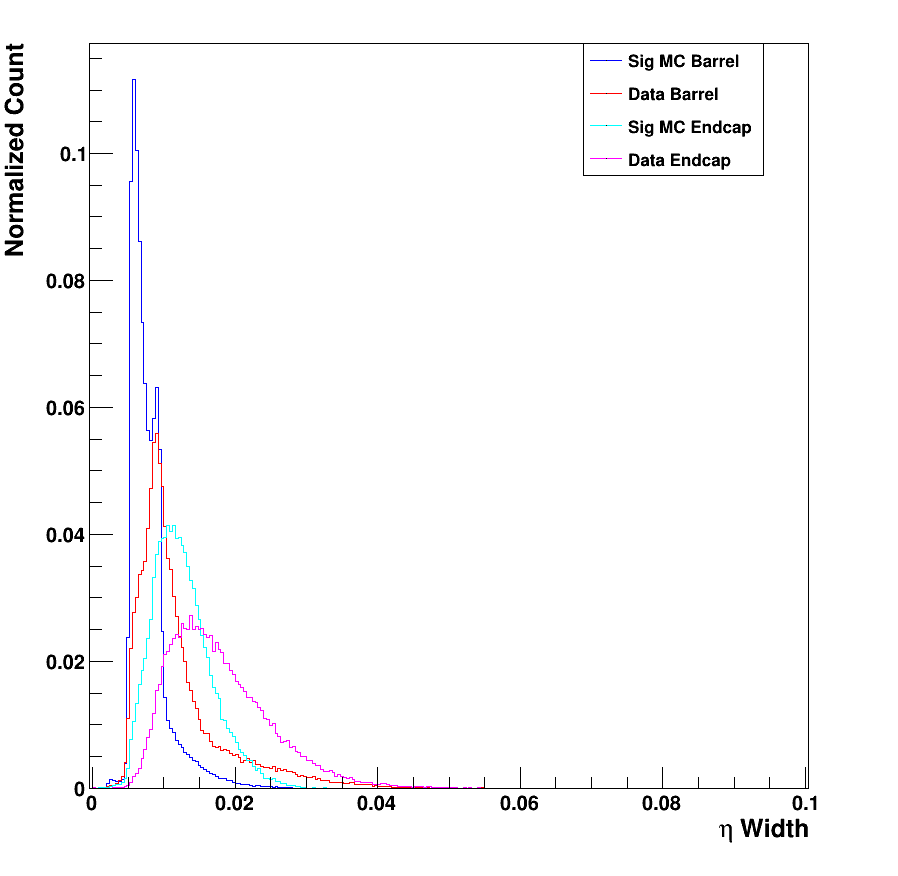
\includegraphics[width=\linewidth]{./Figures/Trigger Training Plots/0713_2026_NormalizedTrainingVars/etaW.png}
		\caption{$\phi$ Width}
		\label{HLTVars:PhiW}
	\end{subfigure}\hfill
	\begin{subfigure}{0.50\linewidth}
		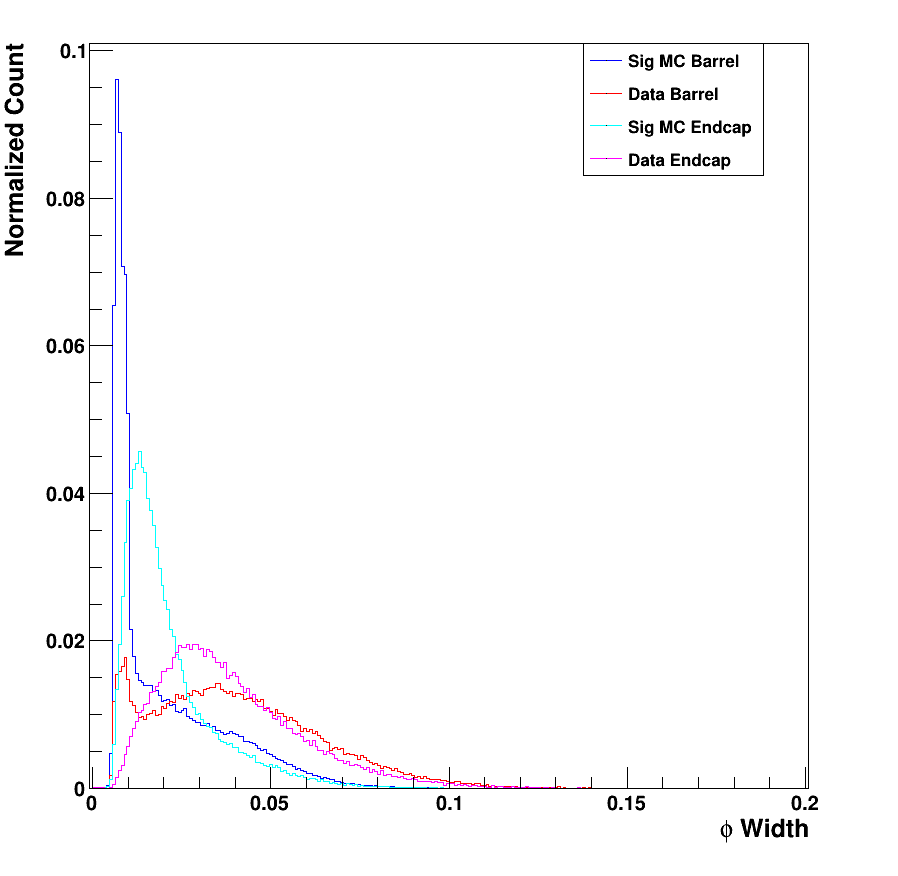
\includegraphics[width=\linewidth]{./Figures/Trigger Training Plots/0713_2026_NormalizedTrainingVars/phiW.png}
		\caption{$\eta$ Width}
		\label{HLTVars:EtaW}
	\end{subfigure}
	\caption{Plots of the $\eta$ and $\phi$ widths. The signal MC is shown in dark blue for the barrel and light blue for the endcap, whereas the data (background) is shown in red for the barrel and pink for the endcap.}
	\label{fig:HLTVars3}
\end{figure}

Next, the $\eta$ and $\phi$ widths (in figure \ref{fig:HLTVars3})are showershape variables that provide further information of the geometric extent of the ECal energy deposition. As with the $\sigma_{i \eta i \eta}$, the expected shapes of these distributions are affected by the crystal geometry -- as a result, the endcap and barrel distributions are expected to differ. Still, the signal MC and data can be seen to show some separation within the barrel and endcap. On average, the data has higher width in both $\eta$ and $\phi$ relative to the signal MC.

\begin{figure}[H]
	\begin{subfigure}{0.50\linewidth}
		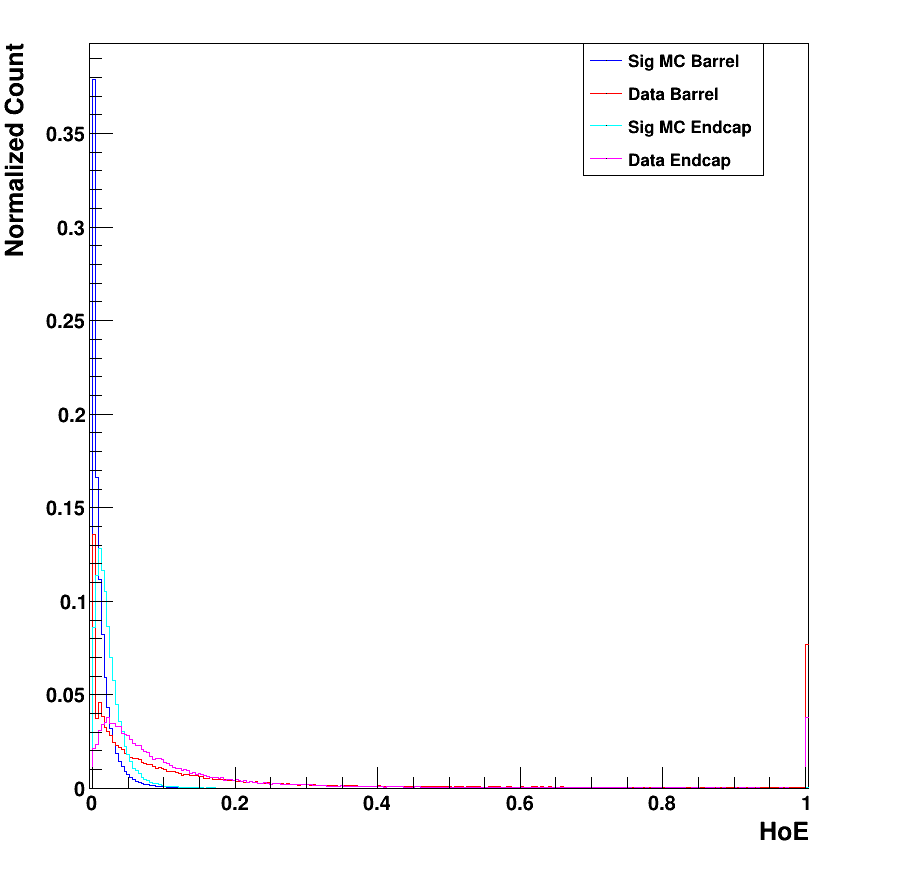
\includegraphics[width=\linewidth]{./Figures/Trigger Training Plots/0713_2026_NormalizedTrainingVars/HoE.png}
		\caption{H/E}
		\label{HLTVars:HoE}
	\end{subfigure}\hfill
	\begin{subfigure}{0.50\linewidth}
		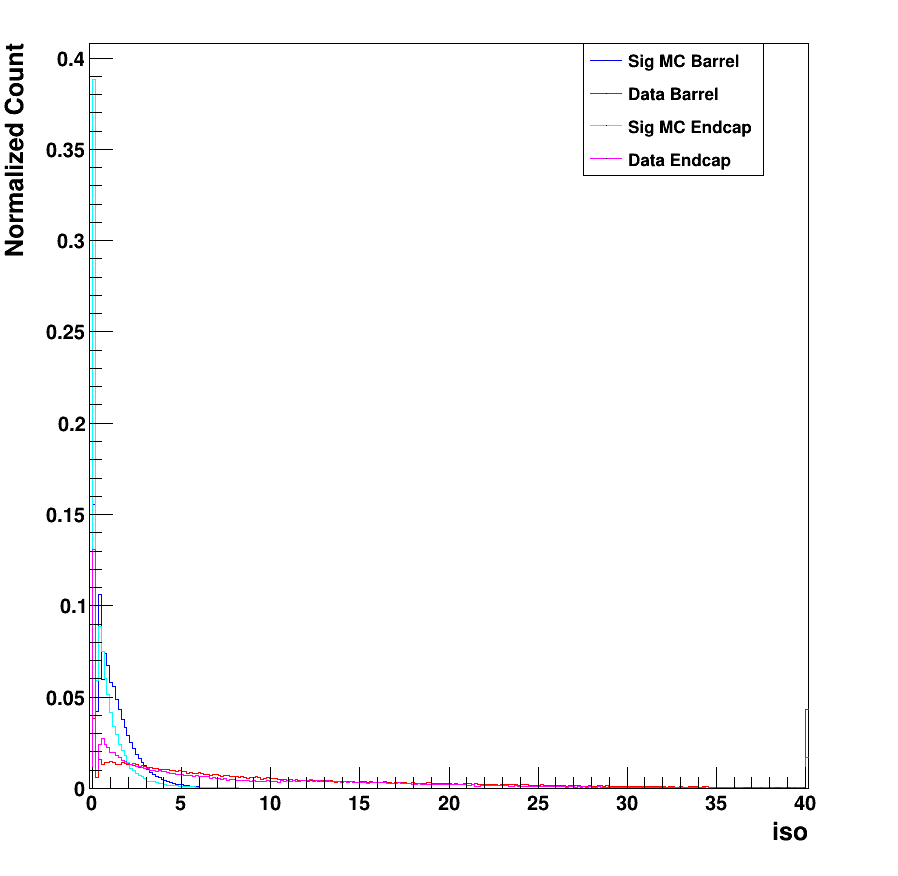
\includegraphics[width=\linewidth]{./Figures/Trigger Training Plots/0713_2026_NormalizedTrainingVars/iso.png}
		\caption{Iso}
		\label{HLTVars:Iso}
	\end{subfigure}
	\caption{Plots of the H/E and isolation. The signal MC is shown in dark blue for the barrel and light blue for the endcap, whereas the data (background) is shown in red for the barrel and pink for the endcap.}
	\label{fig:HLTVars4}
\end{figure}

The H/E in figure \ref{HLTVars:HoE} is a powerful variable for separating photon-like ECal signatures from those originating from QCD jets. Measuring the ratio of how much energy is deposited in the HCal versus the ECal gives some idea of how likely to be a hadronically-produced signature the photon candidate is. Theoretically, a true photon would deposit purely in the ECal, leaving virtually 0 energy signature for the HCal behind it. As a result, real photons should have and H/E near 0. Clearly, the figure shows that this is largely true for the signal MC, whereas the data events -- which are largely composed of jet-like candidates -- have on average much higher H/E values. In fact, there are very few data events with an H/E in the first bin, while nearly 40\% of signal events exhibit this behavior. As a result, this is a very strong separation value for the BDT. 

The isolation, measured in units of energy (GeV), helps measure how much additional energy is deposited outside of the central supercluster. For jet-like events, this value is expected to be higher than true photon signatures; since QCD processes generally produce mutltiple wide jets together, it is expected that much energy will be deposited immediately near the supercluser. Real photons, on the other hand, are more likely to provide a clean energy deposition with little additional surrounding sources of energy. As seen in figure \ref{HLTVars:Iso}, this truth is borne out by the difference between the signal MC and the data. While there are still data events in the first bin near 0 isolation energy, there are nearly 3x as many events in this bin in the signal for both the barrel and endcap. This illustrates the power that this variable provides the BDT.

\subsection{Hyperparameter Tuning}\label{sec:hyperparameters}
Once the input samples and variables are determined, the technical details of the model must by optimized. The structure of the BDTs is determined by the hyperparameters of the model as discussed in chapter \ref{chapter:BDTs}. The most fundamental hyperparameters are the maximum depth, the learning rate, and the total number of trees in the model. The max depth and number of trees directly determine the complexity of the model. A model with more trees will, based on the boosted gradient descent method discussed in chapter \ref{chapter:BDTs}, more precisely estimate the function that maps the chosen input variables from the training sample onto the correct labels of signal versus background. To mitigate the risks of overtraining the model, XGBoost early stopping is used to determine the number of trees. As the software adds additional trees to the ensemble, it measures the chosen objective function at each step on a testing sample not used in the training. Early stopping ends the training of the model when the chosen metric hasn't improved in a chosen number of rounds. For this training, 50 early stopping rounds were used and the area under the curve (AUC) was used as the target metric. So, then, this hyperparameter is essentially fixed while the others must be optimized.

The maximum depth controls the complexity of each individual tree in the ensemble. As discussed in chapter \ref{chapter:BDTs}, the depth determines the number of layers each tree is able to employ. Deeper trees generally allow more precise mapping from input values to output scores at the cost of computation time; each layer of depth constitutes another set of weights that must be computed for each tree. Since it is vital that the computation time is minimized at the trigger level, this is a major consideration. Deeper trees also tend to overfit the training data more, as there are essentially more degrees of freedom with which to fit the mapping function. So, the max depth must be kept as low as possible to avoid both overfitting and unreasonable computation time.

The learning rate controls the size of the individual feature weights from each new tree added to the ensemble. A higher learning rate allows each tree to have higher weights, which will therefore affect the model performance more drastically. Lowering the learning rate makes the model more conservative, as it reduces the overall change to the model predictions provided by each additional tree. Having a higher learning rate generally reduces the number of trees necessary to converge, but decreases the accuracy since statistical fluctuations within each tree can be assigned higher weights. 

It was found that the max depth and learning rate are best optimized in tandem; as the trees become more complex (higher max depth), it was found that making the individual steps more conservative (lower learning rate) led to less overfitting and higher performance. As a result, a 2D grid search was used to optimize these two hyperparameters. A range of both max depth and learning rate was defined, then a model was trained for each combination. The resulting models were appraised in terms of not only their objective scores (AUC and logistic loss in this case, both described in chapter \ref{chapter:BDTs}), but also in terms of the number of trees and the overall model size in megabytes. Since the model must be loaded into RAM at the trigger farm and then the weights applied to each photon in each incoming data event, a model taking up more space will increase both the computation time and memory load at the trigger level. 

After many trials, the best balance of model performance, minimization of overtaining, and model size was found to be a max depth of 7 and a learning rate of 0.25. Experimentally, it was determined that many of the other hyperparameters had minimal impact on the model performance and size, so they were therefore left at their default values.

\section{Determination of BDT Cuts}\label{sec:cutChoices}
After the tuning and training of the model was optimized, a score is generated for each photon in each event. Each event may contain several photon candidates, but the job of the HLT is to determine if any pair of candidates exists that plausibly originates from $H \rightarrow \gamma\gamma$. Given that the BDT was trained such that photons originating from $H \rightarrow \gamma\gamma$ MC are assigned a high score and background processes are given a low score, the photon candidates are first sorted by the output BDT score. Then, the highest two scores can be selected and the values analyzed for both signal MC and data events. 

Since the HLT path simply renders a decision about whether an event contains a $H \rightarrow \gamma\gamma$ process, cuts on the pairs of output scores must be chosen such that the number of signal events kept is maximized (high signal efficiency) while the total number of data events kept is minimized (low trigger rate). 

Below, in figure \ref{fig:HLTOutputScores}, the high and low scores for signal MC are shown at left. Since these are purely signal events, it is expected that the scores to be clustered near 1. As can be seen, the higher of the two scores (along the x axis) tends to be above 0.9 for a large percentage of events. Meanwhile, while the lower of the two scores does cluster above 0.8, there is still a large band of score values extending down to 0. This means that there are many signal events for which one photon has a very high score, but the second photon has a lower score. 

\begin{figure}[H]
	\centering
	\subfloat[SigScores][]{
		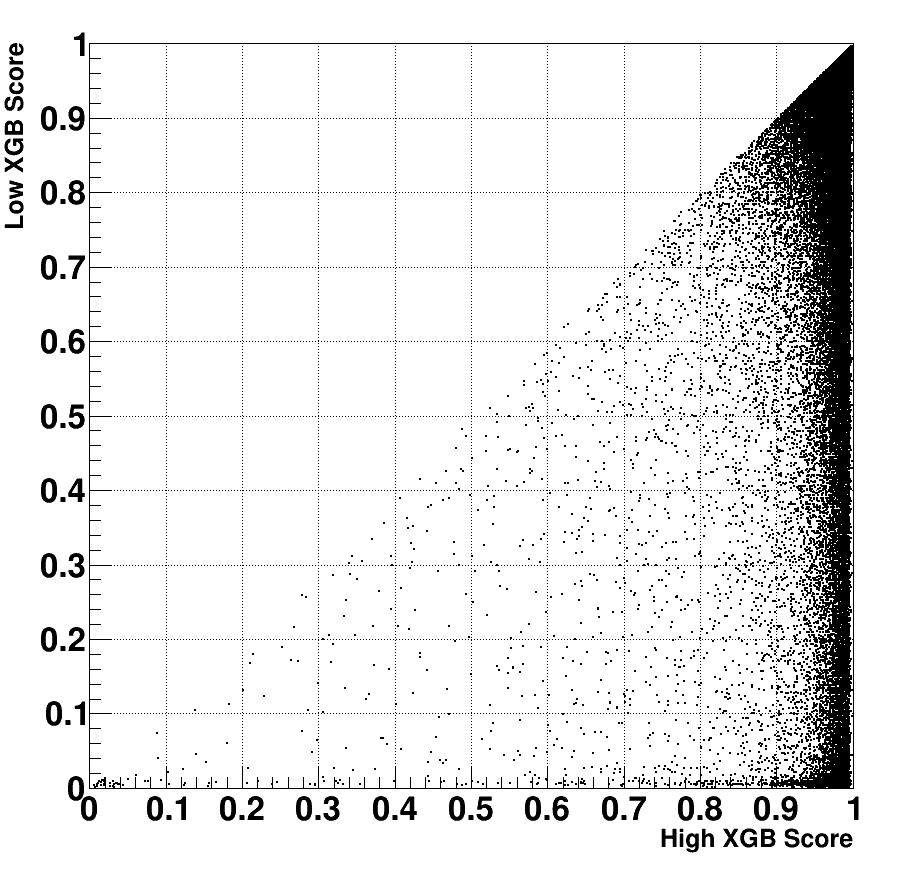
\includegraphics[width=.48\linewidth]{./Figures/Trigger Training Plots/0618_ScorePlotsNoCuts/highandLowScore_XGBCut_M90_Sig_0617_All.png}
	} \hfill
	\subfloat[BkgScores][]{
		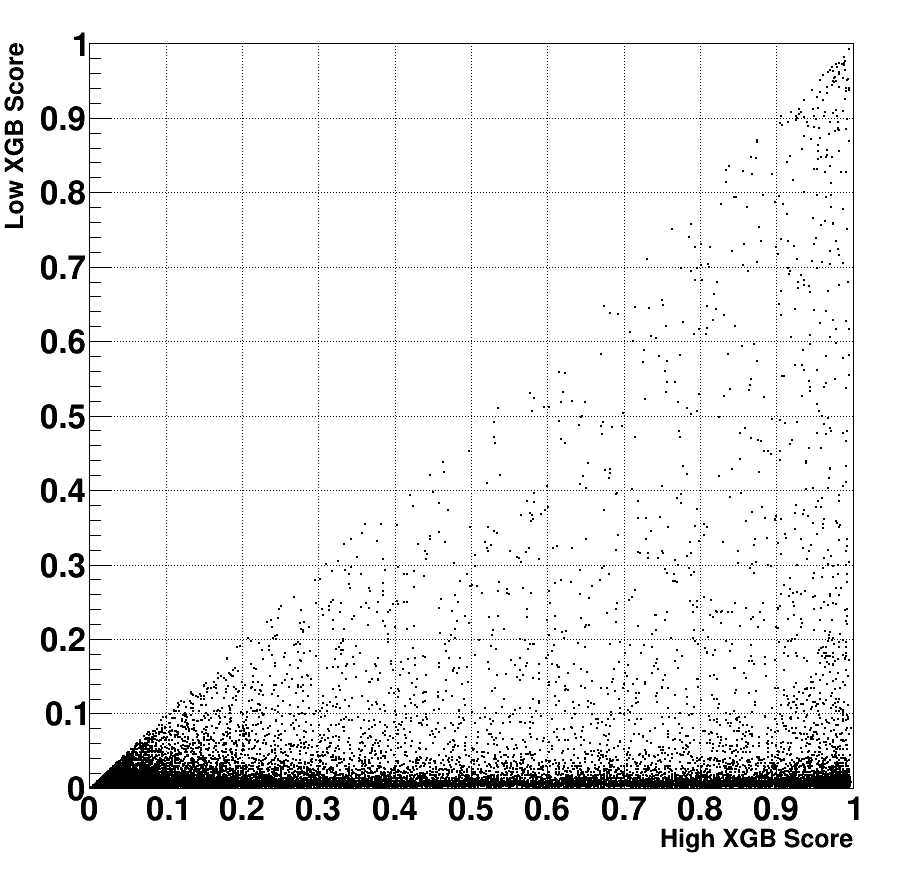
\includegraphics[width=.48\linewidth]{./Figures/Trigger Training Plots/0618_ScorePlotsNoCuts/highandLowScore_XGBCut_M90_Bkg_0617_All.png}
	}
	\caption{XGBoost output scores for two selected photon candidates in the Winter 2024 ggH signal MC. The higher of the two scores is plotted on the X-axis, while the lower of the two is plotted on the Y-axis.}
	\label{fig:HLTOutputScores}
\end{figure}

Next, consider the scores of the data sample shown at right in in \ref{fig:HLTOutputScores}. Given the rarity of $H \rightarrow \gamma\gamma$ events at the trigger level, it is expected that essentially all of these data events correspond to background processes. As a result, the vast majority of these data photon candidates should be assigned a BDT score close to zero. As can be see, the lower of the two photon scores very rarely extends above 0.1. Though the higher of the two scores is often close to 0, there are still many events where the value extends towards 1. Since this BDT is designed to indentify individual photon candidates, it can be inferred that many of these data events have one real photon (which is a major source of background as discussed in section \ref{sec:HLTDataSamples}).

As discussed in section \ref{sec:HLTXGBInfo}, the single photon BDTs are trained separately for photon candidates in the barrel and those in the endcap. Due to the separate trainings -- as well as the differences in kinematics and detector geometry -- the score distributions for barrel and endcap photon candidates are not perfectly equivalent. As a result, the chosen cuts must be tuned separately for the barrel and endcap photons. This presents an issue, as diphoton events may contain two barrel photon candidates (BB), two endcap photon candidates (EE), or one photon candidate in each region of the detector (BE). The simplest way to deal with this is to choose the single photon cuts by reference to the BB and EE distributions, then apply the chosen barrel and endcap cuts to all photons in either region.

Given the shapes of the output distributions in figure \ref{fig:HLTOutputScores}, it is clear that a single cut value for both photons will not achieve maximum signal efficiency. While many of the high score photons are clustered above 0.9, there are still many events with a second photon candidate that has a lower score. In order to preserve these signal events while still removing much of the background, cuts can be selected such that the cut value on the lower score depends on the higher score. For first photons with a very high score, a very loose cut can be applied to the second photon. As the score of the first photon decreases, the cuts on the second photon can be tightened. In the case where the first photon has a relatively low score, a tighter cut is applied on the second photon to help reduce the number of events with two bad photon candidates in the data while still preserving much of the signal. Since the data at the trigger level is strongly dominated by di-jet or single photon events, these cuts can drastically reduce the data rate while still preserving much of the signal. These cuts were experimentally determined, and are tabulated in table \ref{tab:HLTScoreCuts}.

\begin{table}[h]
    \centering
    \caption{Chosen score cuts for BB and EE events}
	\label{tab:HLTScoreCuts}
    \begin{subtable}{.45\textwidth}
        \centering
        \caption{Score cuts for BB events}
        \begin{tabular}{|c|c|}
            \hline
            \textbf{High Score} & \textbf{Minimum Low Score} \\
			\Xhline{2pt}
            0.92 & 0.02 \\ \hline
            0.85 & 0.04 \\ \hline
            0.30 & 0.14 \\ \hline
        \end{tabular}
    \end{subtable}
    \hfill
    \begin{subtable}{.45\textwidth}
        \centering
        \caption{Score cuts for EE events}
        \begin{tabular}{|c|c|}
            \hline
			\textbf{High Score} & \textbf{Minimum Low Score} \\
			\Xhline{2pt}
            0.95 & 0.04 \\ \hline
            0.85 & 0.08 \\ \hline
            0.5 & 0.20 \\ \hline
        \end{tabular}
    \end{subtable}
\end{table}

Events that satisfy these requirements can be plotted on top of figures \ref{fig:HLTOutputScores} . In figure \ref{fig:HLTAcceptedScoresBB} and \ref{fig:HLTAcceptedScoresEE} below, the selected events for BB and EE can be seen, respectively, in red. Yellow lines are added to the plots to demarcate the cuts. These plots contain both the signal MC (left) and the Data (right).

\begin{figure}[H]
	\centering
	\subfloat[][]{
		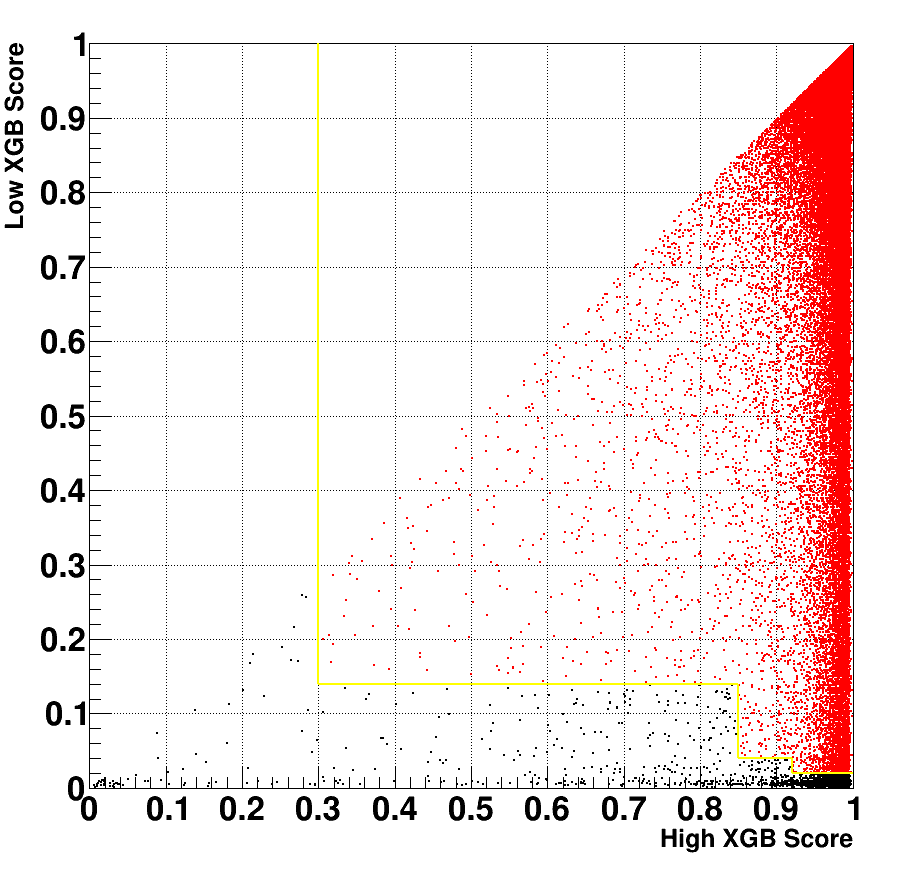
\includegraphics[width=.48\linewidth]{./Figures/Trigger Training Plots/0618_ScorePlotsWithCuts/highandLowScore_XGBCut_M90_Sig_0617_BB.png}
	} \hfill
	\subfloat[][]{
		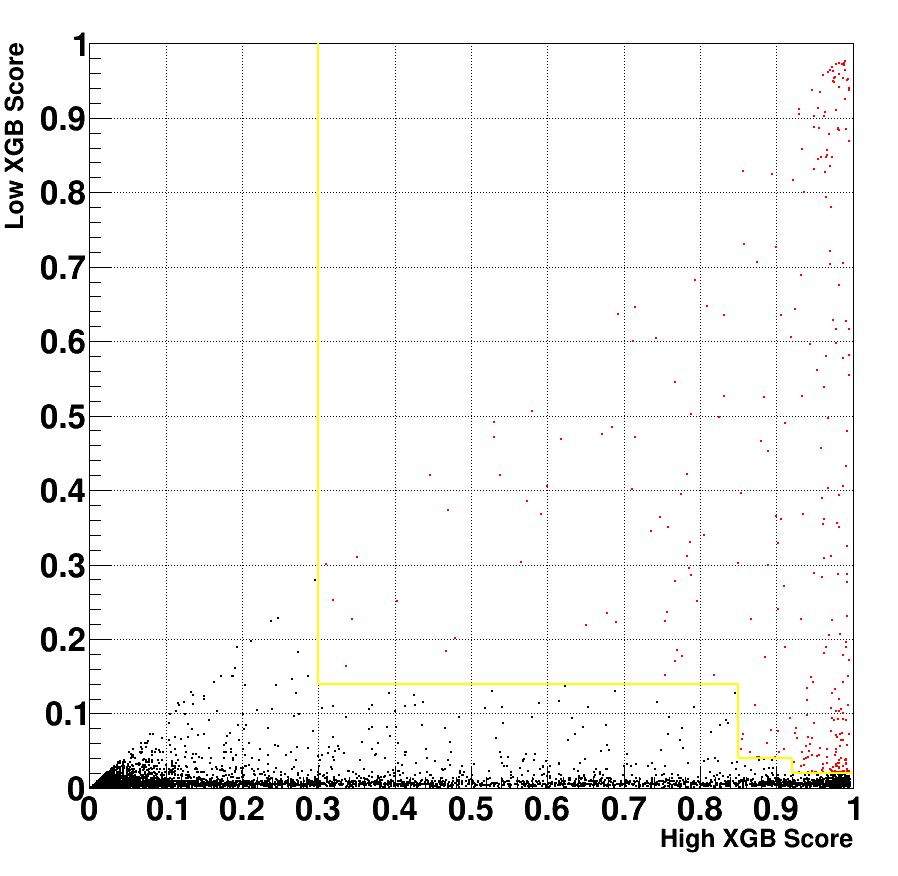
\includegraphics[width=.48\linewidth]{./Figures/Trigger Training Plots/0618_ScorePlotsWithCuts/highandLowScore_XGBCut_M90_Bkg_0617_BB.png}
	}
	\caption{XGBoost output scores for two selected photon candidates in the Winter 2024 ggH signal MC (a), and 2023 Data (b). The higher of the two scores is plotted on the X-axis, while the lower of the two is plotted on the Y-axis.}
	\label{fig:HLTAcceptedScoresBB}
\end{figure}

\begin{figure}[H]
	\centering
	\subfloat[][]{
		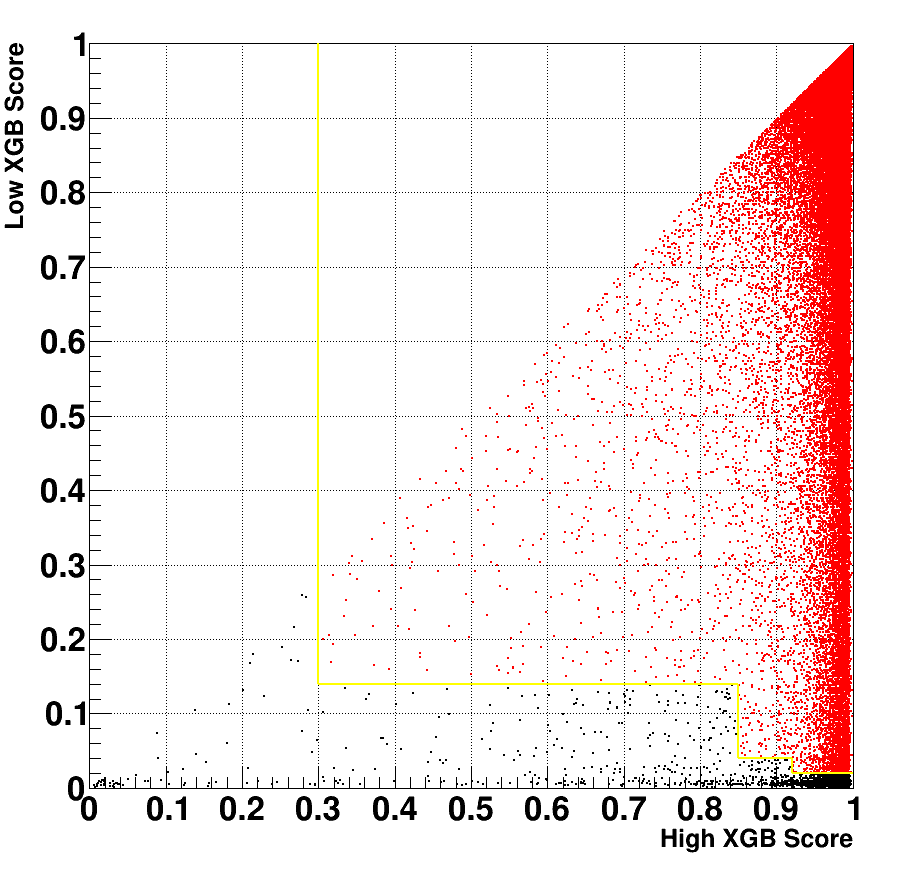
\includegraphics[width=.48\linewidth]{./Figures/Trigger Training Plots/0618_ScorePlotsWithCuts/highandLowScore_XGBCut_M90_Sig_0617_EE.png}
	} \hfill
	\subfloat[][]{
		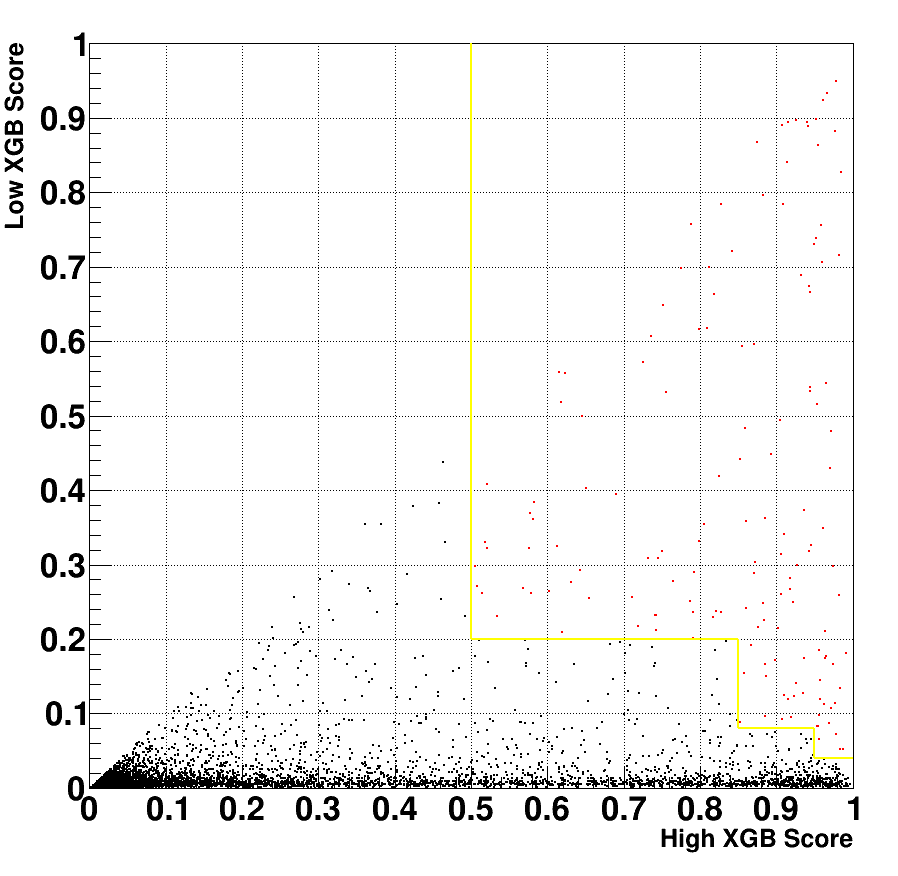
\includegraphics[width=.48\linewidth]{./Figures/Trigger Training Plots/0618_ScorePlotsWithCuts/highandLowScore_XGBCut_M90_Bkg_0617_EE.png}
	}
	\caption{XGBoost output scores for two selected photon candidates in the Winter 2024 ggH signal MC (a), and 2023 Data (b). The higher of the two scores is plotted on the X-axis, while the lower of the two is plotted on the Y-axis.}
	\label{fig:HLTAcceptedScoresEE}
\end{figure}

\section{Evaluation of BDT Cuts}\label{sec:onlineEfficiencies}
This choice of cuts, clearly, is able to preserve much of the signal MC while accepting very few of the data events examined. While the overall signal efficiency and data rate are key metrics to appraise our MVA-HLT, it is also important to examine where in the kinematic phase space events are being gained relative to the standard diphoton HLT. While a more complete measurement of this will be shown in chapter \ref{chapter:Results}, a preliminary analysis can be made with the cuts applied in this initial development framework. 

Below, plots of selected kinematic variables are shown. The events accepted by the current diphoton HLT are shown in green, while the events accepted by the new MVA-HLT are shown in blue. As with the previous score plots, the Winter24 GGH signal MC will be shown at left, whereas the 2023 Data will be shown at right.

\begin{figure}[H]
	\centering
	\subfloat[][]{
		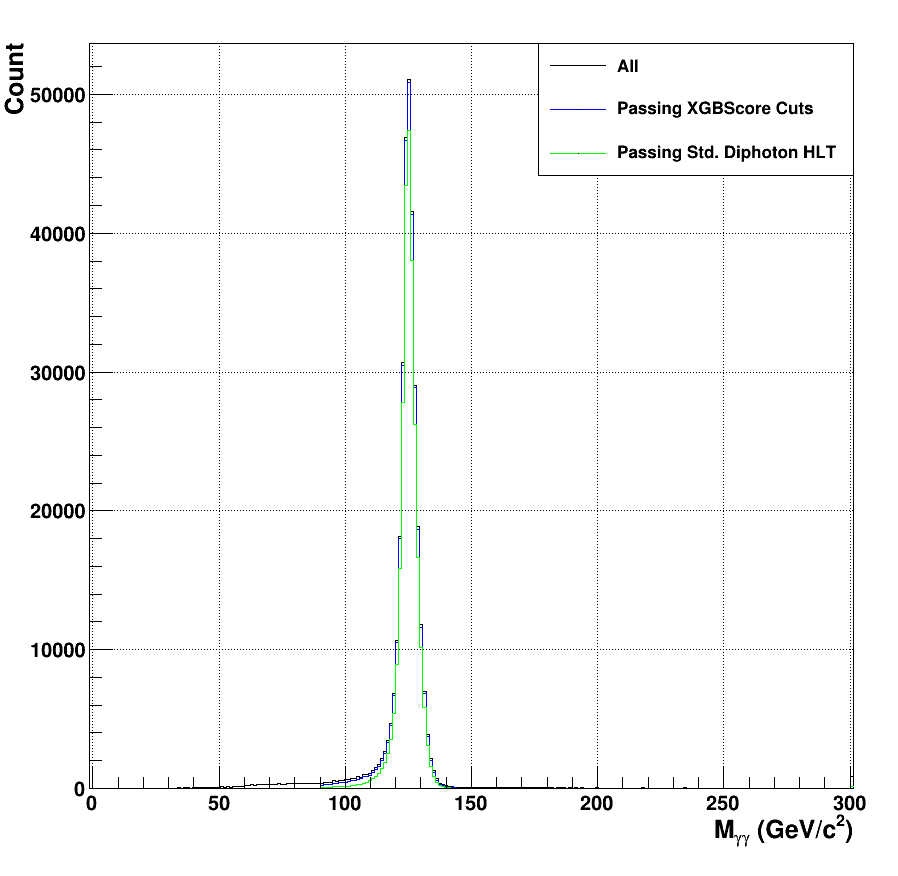
\includegraphics[width=.6\linewidth]{./Figures/Trigger Training Plots/0618_OnlineValidationPlots/mass_All_Sig.png}
	} \hfill \\
	\subfloat[][]{
		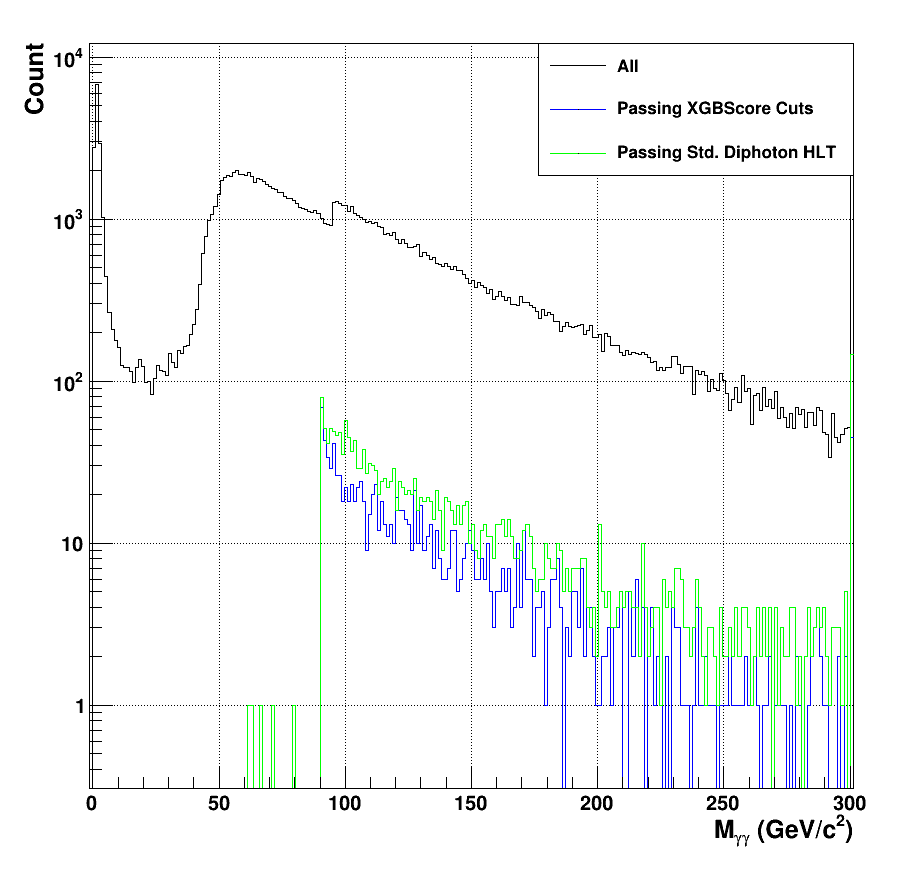
\includegraphics[width=.6\linewidth]{./Figures/Trigger Training Plots/0618_OnlineValidationPlots/mass_All_Bkg.png}
	}
	\caption{Diphoton mass for the signal MC (a) and data (b). Events accepted by the MVA-HLT are shown in blue, while events accepted by the standard HLT are shown in green.}
	\label{fig:HLTAcceptedMass}
\end{figure}


Beginning with the mass, it can immediately be seen that MVA-HLT accepts 94.2\% of signal MC events, which is an approximately 13.6\% relative gain in signal efficiency compared to the 82.9\% acceptance of the standard diphoton HLT. Additionally, the data rate appears considerably lower; while the standard HLT accepts 1.44\% of the analyzed events, the MVA-HLT only accepts 0.86\%, which corresponds to a 40.3\% reduction in data rate. 

One major consideration when examining the mass is the measured mass width of the accepted signal events. Generally, a more narrow peak is considered a cleaner signal. By treating the mass distribution as approximately gaussian, the width can be easily understood by measuring the standard deviation. Since the distribution is only approximately gaussian, it is safer to instead construct the quantity $2\sigma_{effective}$, which is simply the width (in $GeV/c^{2}$) that contains 95\% of the peak. Although this is not a statistically rigorous construct, it can be used to compare the approximate shapes of similar distributions in an interally consistent way. It can be seen that the $2\sigma_{effective}$ is marginally increased for the MVA-HLT, reaching 6.58 compared to the 6.07 of the events accepted by the standard trigger. Some increase in width is to be expected, as accepting more events will necessarily bring the distribution closer to the "all" curve that has a wider width than either selection. 

(Statments about the background mass distribution?)

\begin{figure}[H]
	\centering
	\subfloat[][]{
		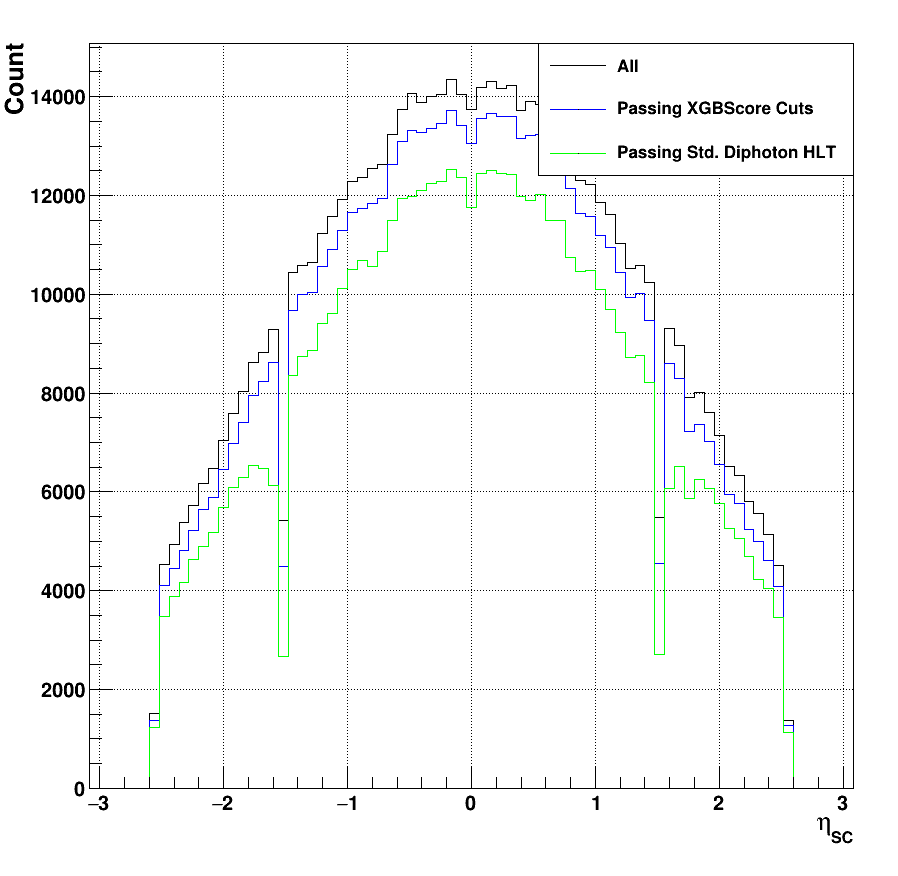
\includegraphics[width=.60\linewidth]{./Figures/Trigger Training Plots/0618_OnlineValidationPlots/eta_All_Sig.png}
	} \hfill \\
	\subfloat[][]{
		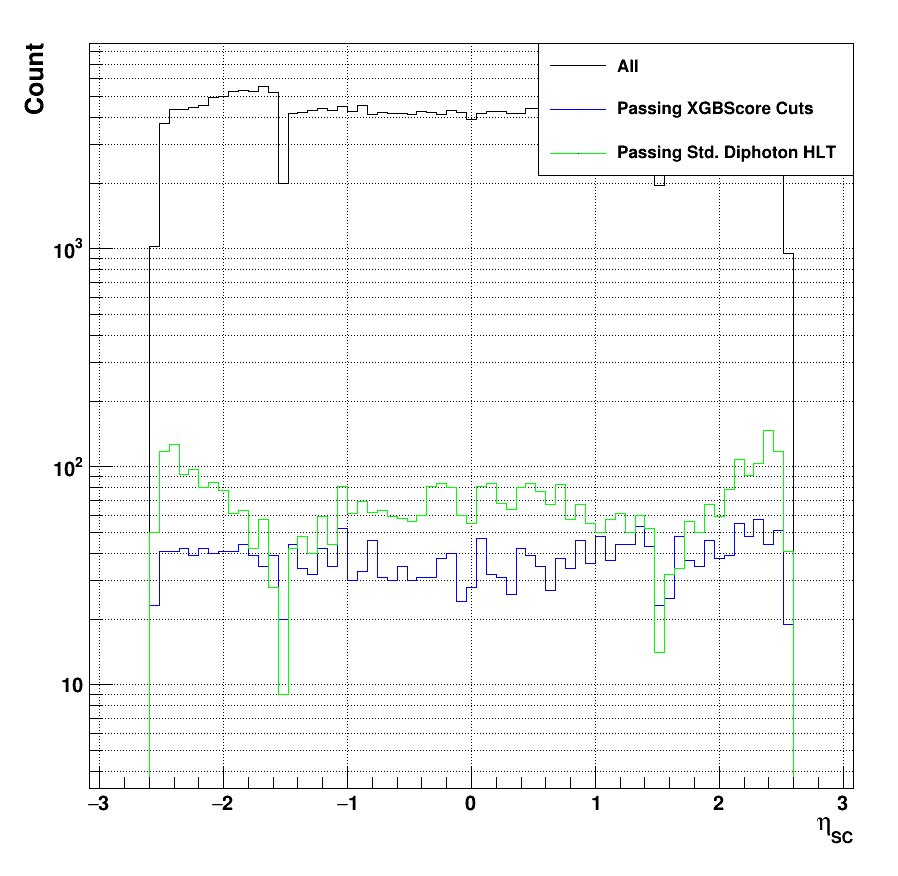
\includegraphics[width=.60\linewidth]{./Figures/Trigger Training Plots/0618_OnlineValidationPlots/eta_All_Bkg.png}
	}
	\caption{Photon $\eta$ for the signal MC (left) and data (right). Events accepted by the MVA-HLT are shown in blue, while events accepted by the standard HLT are shown in green.}
	\label{fig:HLTAcceptedEta}
\end{figure}


Above, the next kinematic variable shown is the $\eta_{sc}$ of both photons plotted together. As seen in both signal and background, the separation between the ECal Barrel (EB) and ECal Endcap (EE) can be seen at $\eta_{sc} \approx \pm 1.5$. For the signal, thoughout the barrel, both the MVA-HLT and standard HLT accept photon candidates in relatively constant propotion to the total distribution, though the MVA-HLT has overall improved acceptance. While the MVA-HLT still has relatively constant acceptance in the EE, it can immediately be seen that the standard HLT is excluding many events in the lowest-$\eta_{sc}$ region of the endcap. Investigations have shown that this is due to the $R_{9}$ cuts made within the trigger. This represents a reduction in kinematic coverage for the standard HLT, whereas the MVA-HLT is able to resolve this issue and maintain maximum kinematic coverage. 

Considering the background, it can immediately be seen that the MVA-HLT has a relatively flat acceptance in both the EB and EE, while the standard HLT appears to accept more data at the extreme-$\eta_{sc}$ reigions of the endcap. As can be seen from the  MC, this region tends to contain less of the $H \rightarrow \gamma \gamma$ signal events and therefore represents a lower signal to background ratio. 


\begin{figure}[H]
	\centering
	\subfloat[][]{
		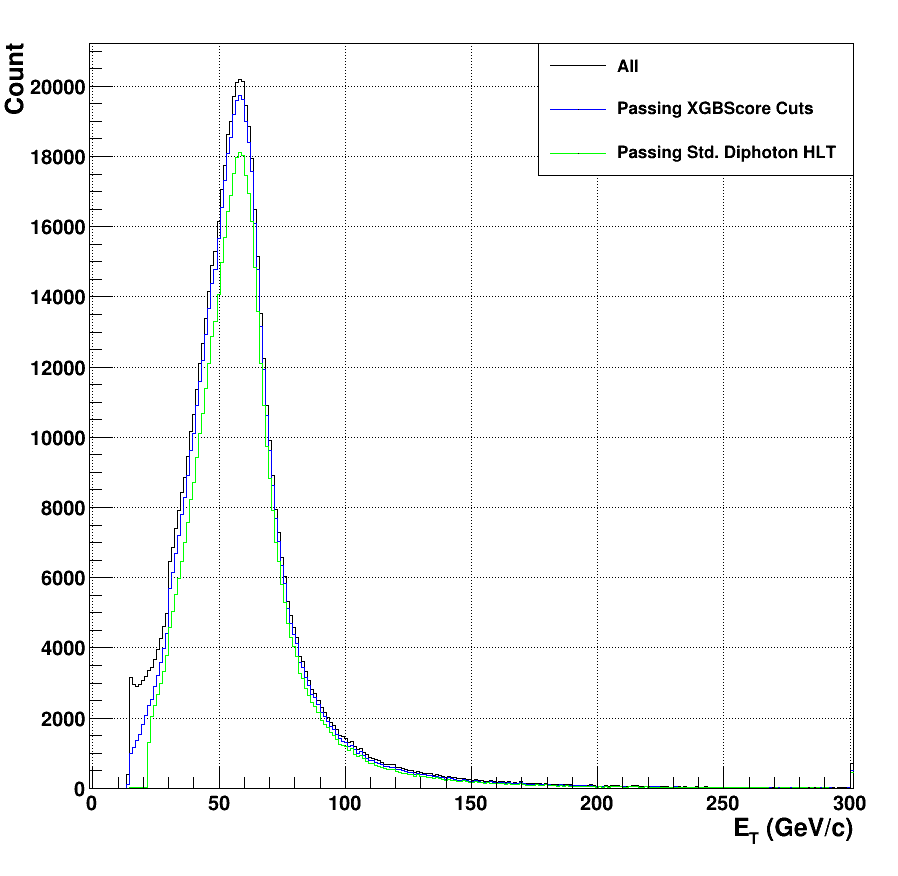
\includegraphics[width=.60\linewidth]{./Figures/Trigger Training Plots/0618_OnlineValidationPlots/et_All_Sig.png}
	} \hfill \\
	\subfloat[][]{
		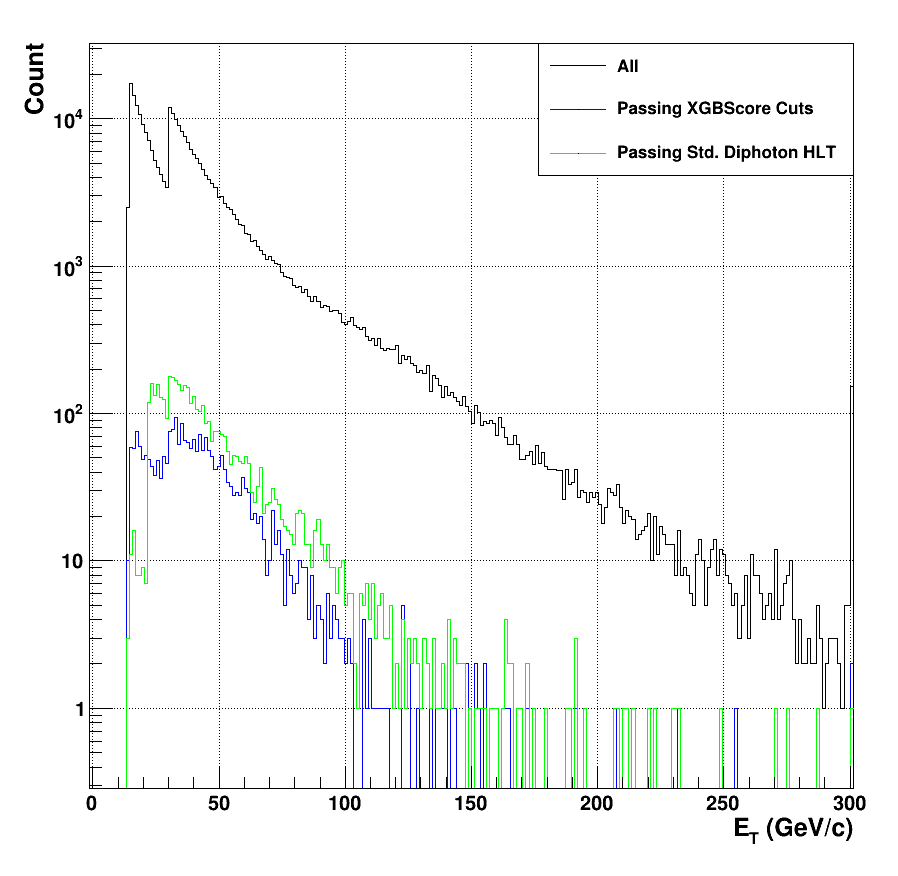
\includegraphics[width=.60\linewidth]{./Figures/Trigger Training Plots/0618_OnlineValidationPlots/et_All_Bkg.png}
	}
	\caption{Photon $E_T$ for the signal MC (left) and data (right). Events accepted by the MVA-HLT are shown in blue, while events accepted by the standard HLT are shown in green.}
	\label{fig:HLTAcceptedEt}
\end{figure}


Finally, consider the transverse energy of the photon candidates, $E_T$. Here, both candidates are again shown on the same plot, which explains the double-peaking behavior in the background distribution. The standard diphoton HLT contains cuts at 30 and 22 $GeV2$ for the lead and sublead photon, respectively. The sublead cut can clearly be seen in both the signal, at left, and the background at right. While the new MVA-HLT selection accepts more of these low-$E_T$ photons, it is clear that little of the gain comes from this kinematic region. Below about 30 $GeV$, both selections tend to cut out many photons from the total distribution. In the case of the MVA-HLT, this is likely due to those photon candidates being of lower quality and therefore being assigned a lower BDT score.

Below, in table \ref{tab:HLTEffs}, the acceptance percentages are given for the 3 different diphoton $\eta_{sc}$ 
configurations, as well as the total acceptance for both signal and background, compared to the standard HLT cuts.

\begin{table}[h]
    \centering
    \caption{Signal efficiencies and background acceptances for both triggers, broken down by diphoton $\eta_{sc}$}
	\label{tab:HLTEffs}
    \begin{subtable}{.49\textwidth}
        \centering
        \caption{Signal Efficiencies}
        \begin{tabular}{|c|c|c|}
            \hline
            \textbf{Region} & \textbf{MVA-HLT(\%)} & \textbf{Std. HLT(\%)}\\
			\Xhline{2pt}
            B-B & 95.93 & 89.32\\ \hline
            B-E & 91.91 & 74.10\\ \hline
            E-E & 89.46 & 76.85\\ \hline
            All & 93.86 & 82.64\\ \hline
        \end{tabular}
    \end{subtable}
    \hfill
	\begin{subtable}{.49\textwidth}
        \centering
        \caption{Data Acceptances}
        \begin{tabular}{|c|c|c|}
            \hline
            \textbf{Region} & \textbf{MVA-HLT(\%)} & \textbf{Std. HLT(\%)}\\
			\Xhline{2pt}
            B-B & 0.65 & 1.06\\ \hline
            B-E & 1.20 & 2.17\\ \hline
            E-E & 0.58 & 1.07\\ \hline
            All & 0.88 & 1.56\\ \hline
        \end{tabular}
    \end{subtable}
\end{table}
\section{Final Implementation in HLT Menu} \label{sec:HLTImplementation}
As discussed in section \ref{sec:TriggerSoftware}, triggering and event reconstruction is handled by the distributed CMSSW software framework. As a result, any proposed trigger developments must be deployed in a central CMSSW release. While the software strategy is the same as the original python implementation, the code must of couse be rewritten in C and adapted to work within the trigger.

As described in section \ref{sec:HLT}, the HLT operates on all photon candidates in an event, then simply renders an event-by-event decision if any pair of photons satisfy the chosen conditions. As a result, the first step of the implementation is to create a module that calculates the BDT score for each photon candidate in every event. Once these scores are stored within the trigger path, another module must be constructed to check if any possible pair of photon candidates passes the two-fold cuts described above. Importantly, due to the constraints on storage space, the scores of the individual photon candidates cannot be saved to the event. As a result, the only output from the MVA-HLT is a decision on whether the event should be accepted or rejected.

Luckily, these two modules are the only software additions required to add the BDT to the trigger menu. Beyond that, standard modules can be used (with some modifications to the cuts made) within ConfDB to construct the entire trigger path as discussed in section \ref{sec:confDB}. The first step of the HLT path is to require the necessary L1 triggers. The standrd L1 suite required by the existing HLT is used here, which consistes of a combination of single and double EGamma triggers as described in section \ref{sec:L1}. 

In order to reduce the amount of MVA scores that must be calculated, the very loose kinematic cuts are applied to all photon candidates in the event as the first step. While these cuts are quite loose, they still serve to reduce the number of candidates considered. Since many data events may have many photon candidates, this will help reduce the time taken to calculate the BDT scores. (Is this true? Do individual photon candidates get removed at the HLT level, or just events?)

With the preliminary cuts in place, the module that calculates the scores is placed in the HLT path, followed by the module that makes the cuts as described in section \label{cutChoices}. Finally, a combined module is created that combines these BDT cuts on both photons with a mass cut of $M_{\gamma \gamma} > 90 GeV/c^{2}$. So, then, the whole HLT path serves to check if there is any possible pair of photon candidates that passes the loose kinematic cuts, the pairwise BDT cuts, and the $M_{\gamma \gamma}$ cut. If any pair satisfies these conditions, a flag is added to the event and all photon candidates are kept at the RAW level. 

\chapter{MVA-Based Offline Preselection} \label{chapter:OfflineSelection}
As discussed in chapter \ref{chapter:Software}, the HLT is one of the first steps in selecting data and MC events for analysis. Once a decision has been rendered by the HLT, the event is read out and saved in either the appropriate data stream or in the corresponding MC sample. Once these files are read in by the analysis software -- in this case HiggsDNA as described in section \ref{sec:HiggsDNA} -- further selection cuts are made to create a final analysis sample on which measurements can be made. 

\section{Current Diphoton Preselection}\label{sec:StandardPresel}
The current diphoton selection is created by direct analogy to the standard diphoton HLT; firstly, $p_T$, showershape, and isolation cuts are made on individual photons in an event, then the single photons are paired together and cuts are made on the resulting diphoton. In the case of the HLT, a simple diphoton mass cut is made. At the offline analysis level, however, the diphoton cuts are made on $p_T/M_{\gamma \gamma}$. 

The $H \rightarrow \gamma \gamma$ preselection is described in detail in \cite{Run2Hgg2018}. First, loose cuts of $p_T > 20 GeV/c$, $R_9 > 0.5$, $H/E < 0.08$, and $idMVA > 0.9$ are applied to each photon candidate. Additionally, the $ \lvert \eta_{sc} \rvert$ is constrained to be below 2.5, and the gap region between the EB and EE is excluded (1.444 $< \lvert \eta_{sc} \rvert <$ 1.556). Additionally, the electron veto is required to exclude photons origininating from electron tracks. Beyond that, the remaining isolation and showershape cuts are only applied on low-$\eta$ photons. Above $R_9 = 0.85$ in the barrel and $R_9 = 0.90$ in the endcap, no further preselection cuts are applied. For photons below these $R_9$ thresholds, cuts are applied on the $\sigma_{i\eta i \eta}$, photon isolation, and track isolation. Finally, the electron veto (described in REF) is required for each photon candidate. This veto decision is designed to identify and remove energy signatures associated with a track, which are likely to be electrons.

Once these single photon preselection cuts are applied, all remaining photon canidates are paired together into a collection of diphotons. For each pair, the higher of the two photons must satistfy $p_T > 35 GeV/c$. Paired with the baseline requirement of $p_T > 25 GeV/c$, these cuts closely mimic the 30 and 22 GeV/c cuts applied at the trigger level. Then, the $p_T/M_{\gamma \gamma}$ cuts are applied to the diphoton pairs. At this point, many of the possible photon combinations have been removed. A final diphoton combination must be selected, however, as HiggsDNA is designed to output a single photon pair of photons. The remaining pairs in the event are sorted by their diphoton $p_T$, and the pair with the highest value is written out into the event \cite{Run2Hgg2018}. These cuts, in their totality, are shown in table \ref{tab:PreselCuts}
\begin{table}
	\centering
	\caption{Table showing the cuts applied by the standard preselection for $H \rightarrow \gamma \gamma$.}
	\label{tab:PreselCuts}
	\begin{tabular}{| c | c | c | c | c | c | c |} 
		\hline
		\textbf{Region} & \textbf{$R_9$} & \textbf{H/E} & \textbf{idMVA} & \textbf{$\sigma_{i \eta i \eta}$} & \textbf{$\mathcal{I}_{Pho}$} (GeV) & \textbf{$\mathcal{I}_{Track}$} (GeV)\\
		\Xhline{2pt}
		Barrel & [0.5,0.85] & $<$ 0.08 & $'
		>$ 0.9 & $<$ 0.015 & $<$ 4.0 & $<$ 4.0\\
		 & $>$ 0.85 & $<$ 0.08 & $>$ 0.9 & -- & -- & --\\
		Endcap & [0.5,0.9] & $<$ 0.08 & $>$ 0.9 & $<$ 0.035 & $<$ 4.0 & $<$ 4.0\\
		 & $>$ 0.9 & $<$ 0.08 & $>$ 0.9 & -- & -- & --\\ 
		\hline
	\end{tabular}
\end{table}

In addition, there are cuts on the $p_T/M_{\gamma \gamma}$ applied as part of what are termed the Standard Analysis(SA) cuts. These are kept separate from the single photon preselection cuts, as some analyses may want to make adjustments to them. For the Run 3 preselection, a geometric mean $p_T/M_{\gamma \gamma}$ cut is used \cite{Run3Hgg2025}. The cut on the second (sublead) photon is straightforward, at $p^{\gamma1}_T/M_{\gamma \gamma} > 1/4$. The second cut, however, uses the geometric mean of the two $p_T$ values as $\sqrt{p^{\gamma1}_T p^{\gamma2}_T }/M_{\gamma \gamma} > 1/3$. There is no explicit $M_{\gamma \gamma}$ cut applied within the preselection, as the possibility for high- and low-mass Higgs analysis is left open. For the purposes of comparing this preselection to the new MVA-based selection, only the standard mass Higgs is considered. So, a loose cut of $90 < M_{\gamma \gamma} < 180 GeV/c^2$ is applied to all resulting diphotons.

\section{Development of MVA-Based Offline Preselection}
Since the offline selection is designed to cover the HLT used, it is clear that applying the preexisting preselection described above on top of the MVA-HLT is a suboptimal strategy. In fact, since these cuts mirror the standard HLT quite closely, it is expected that applying the standard preselection on top of the MVA-HLT would likely reduce or even entirely remove the signal efficiency gains obtained by the new trigger. As a result, an alternative set of preselection cuts must be proposed that allows the trigger-level gains to be realized at the offline analysis level. 

Just as the standard preselection cuts are designed to not only cover the standard HLT but work in much the same way, a new preselection can be created with maximum similarity to the MVA-HLT. One major complication of this is that the same BDTs cannot be used for both the trigger and offline selection. Since the reconstruction differs for the NanoAOD vs the RAW, the input variable distributions will be different enough that the models are not directly comperable. Instead, a new BDT-based preselection framework must be developed and its coverage of the MVA-HLT must be analyzed.
\subsection{Creation of Single Photon BDTs}
\subsubsection{A $\gamma + Jet$ BDT}
As discussed in section \ref{sec:StandardPresel}, there already exists an MVA within the standard preselection. While this idMVA is now a centralized part of the NanoAOD format, historical preselections used an MVA trained of $\gamma + Jet$ MC (REF?). Events in $\gamma + Jet$ MCs will contain one real (prompt) photon and one jet that looks like a photon, termed a "fake". This MC provides a very easy-to-use training sample, as one can simply use the prompt $\gamma$ as the signal photon and the fake as the background photon. This standard $\gamma + Jet$ idMVA is usually only used to make relatively loose cuts as part of the much broader preselection cuts as described above. 

The original idMVA was trained using many of the variables from the preselection as input variables. These same input variables were used as a starting point for a new $\gamma + Jet$ MVA, with the addition of H/E. By adding this variable to the inputs, the new $\gamma + Jet$ MVA contains the same information available to the standard preselection described above. Additionally, this allows the offline selection model to more closely mirror the MVA-HLT. The input variables used are shown below in table \ref{tab:OfflineSinglePhoInputVars}. As with the MVA-HLT, the barrel and endcap models are trained separately, with individual photons selected based on their location in the detector.

\begin{table}
	\centering
	\caption{Table of input variable names for the offline $\gamma + Jet$ MVA, and a short description of each. The final two variables are only used for training the endcap.}
	\label{tab:OfflineSinglePhoInputVars}
	\begin{tabular}{ | c | c | } 
		\hline
		\textbf{Variable Name} & \textbf{Description} \\
		\Xhline{2pt}
	  	Raw Energy & The total energy deposited in the 5x5 supercluster  \\ 
		\hline
		$R_{9}$ & \makecell{The proportion of the energy contained in the central 3x3 crystals \\ relative to the raw energy}  \\ 
		\hline
		$S_{4}$ & \makecell{The proportion of the energy contained in the central 2x2 crystals \\ relative to the raw energy}  \\ 
		\hline
		$\sigma_{i \eta i \eta}$ & The covariance in terms of crystal spacing ($i_{\eta}$)\\ 
		\hline
		$cov(i \eta i \phi)$ & The covariance between the $\eta$ and $\phi$ coordinates\\ 
		\hline
		$\eta_{SC}$ & The eta coordinate of the center of the supercluster  \\ 
		\hline
		$\eta$ Width &  The supercluster width in $\eta$ \\ 
		\hline
		$\phi$ Width &  The supercluster width in $\phi$ \\ 
		\hline
		H/E & \makecell{The ratio of the total supercluster energy measured in the HCal \\ to that measured in the ECal}  \\ 
		\hline
		PhoIso03 & The photon isolation\\ 
		\hline
		\makecell{Charge Iso \\ w.r.t. Worst Vertex} & \makecell{The charged isolation for the worst vertex determined \\ by the vertexing algorithm}\\ 
		\hline
		\makecell{Charge Iso \\ w.r.t. Chosen Vertex} & \makecell{The charged isolation for the chosen vertex determined \\ by the vertexing algorithm}\\ 
		\hline
		$\rho$ & The event energy density\\ 
		\hline
		\hline
		esEffSigmaRR & temp\\ 
		\hline
		esEnergyOverRawE & temp\\ 
		\hline
	\end{tabular}
\end{table}

As with the trigger level BDT, the sparation between the signal and background in the various input variables can be examined. For the subsequent plots (\ref{fig:GJetVars1}-\ref{fig:GJetVars7}), the prompt and fake will be shown for both the barrel and endcap, as the trainings are separated. The prompt photons will be shown in dark and light blue for the barrel and endcap, respectively. The fake distributions will be shown in red and pink for the barrel and endcap, respectively. All the input variable distributions have been normalized to 1, so that their shapes can be directly compared.


The SC raw energy, in \ref{GJetVars:RawE}, shows rather clear separation for both the barrel and endcap. It can be seen that the prompt photons tend, on average, to have higher total supercluster energy than the fake photons. The separation in $\eta_{SC}$, however, is primarily seen in the endcap, where the fake photons tend towards the higher values. Since the BDT works by creating correlations between variables, and the $\eta_{SC}$ is a strongly kinematic-dependent variable, it will still be shown to be a relatively powerful discrimination variable. 

\begin{figure}[H]
	\begin{subfigure}{0.50\linewidth}
		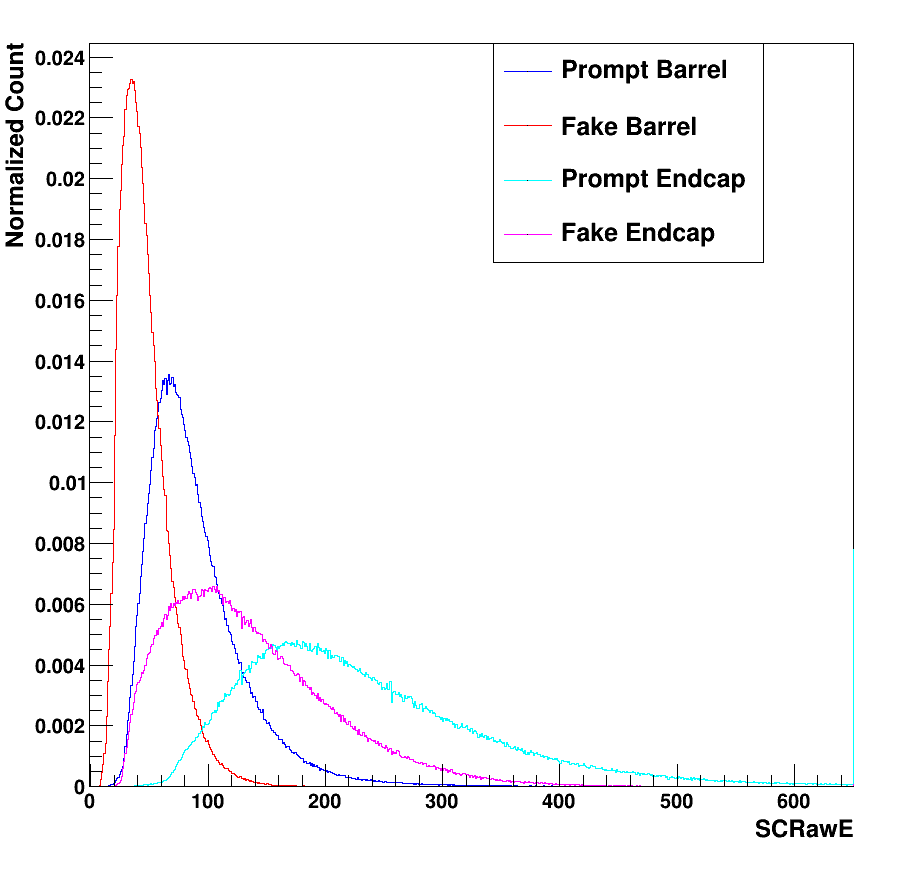
\includegraphics[width=\linewidth]{./Figures/Offline Selection Plots/0709_Updated_GJet_TrainingPlots/SCRawE.png}
		\caption{Raw Energy}
		\label{GJetVars:RawE}
	\end{subfigure}\hfill
	\begin{subfigure}{0.50\linewidth}
		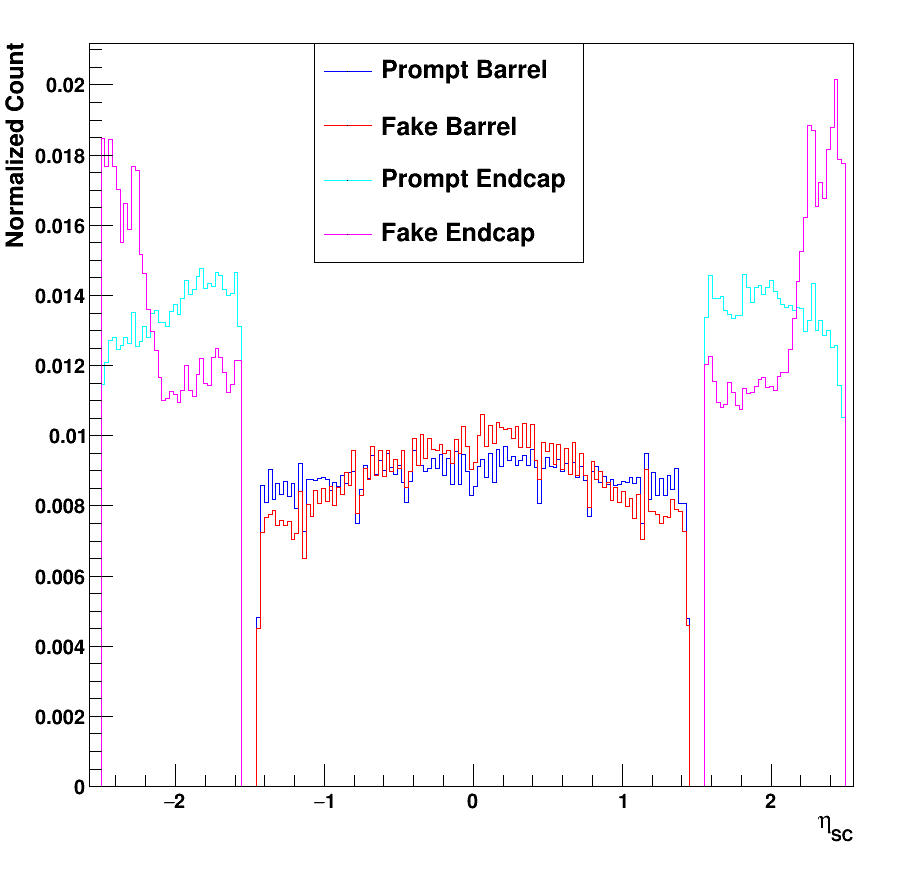
\includegraphics[width=\linewidth]{./Figures/Offline Selection Plots/0709_Updated_GJet_TrainingPlots/scEta.png}
		\caption{$\eta_{SC}$}
		\label{GJetVars:eta}
	\end{subfigure}
	\caption{Plots of the Supercluster raw energy and $\eta_{SC}$. The prompt signal is shown in dark blue for the barrel and light blue for the endcap, whereas the fake background is shown in red for the barrel and pink for the endcap.}
	\label{fig:GJetVars1}
\end{figure}

Next, the energy ratios, $R_9$ and $S_4$ can be examined. It is expected that a real (prompt) photon will have relatively well-localized energy; since the photon is a relatively clean signal in the detector, it is expected that most of the energy will be deposited in the center of the supercluster. It is clear that this is the case for both the barrel and endcap, as seen in figure \ref{fig:GJetVars2}. Since the fake photon corresponds to a jet, it is expected that the energy deposition will be more spread in the supercluster, which can also be seen in the plots. As a result, $R_9$ and $S_4$ can be relativelty powerful discrimination variables. 

\begin{figure}[H]
	\begin{subfigure}{0.50\linewidth}
		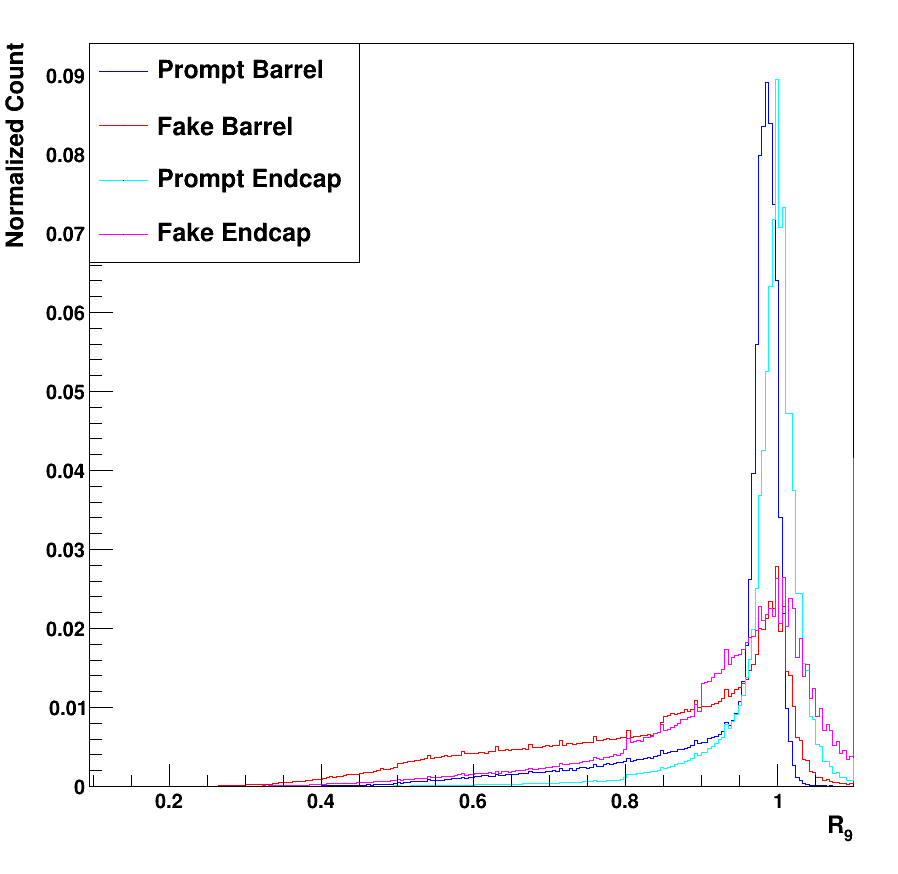
\includegraphics[width=\linewidth]{./Figures/Offline Selection Plots/0709_Updated_GJet_TrainingPlots/r9.png}
		\caption{$R_9$}
		\label{GJetVars:r9}
	\end{subfigure}\hfill
	\begin{subfigure}{0.50\linewidth}
		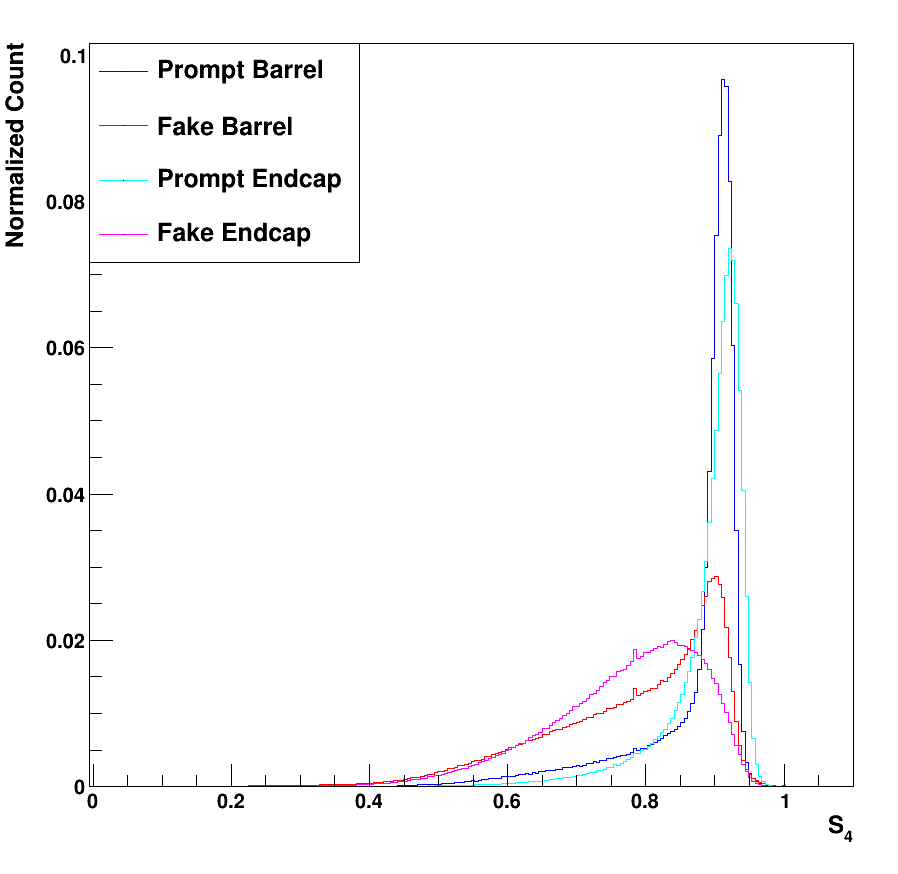
\includegraphics[width=\linewidth]{./Figures/Offline Selection Plots/0709_Updated_GJet_TrainingPlots/s4.png}
		\caption{$S_4$}
		\label{GJetVars:s4}
	\end{subfigure}
	\caption{Plots of the $R_9$ and $S_4$. The prompt signal is shown in dark blue for the barrel and light blue for the endcap, whereas the fake background is shown in red for the barrel and pink for the endcap.}
	\label{fig:GJetVars2}
\end{figure}

The next showershape variables, $\sigma_{i \eta i \eta}$ and cov($i \eta i \phi$), provide information about the energy depositions in terms of the crystal spacing. $\sigma_{i \eta i \eta}$ quantifies the standard deviation of the energy depisited in terms of the $\eta$ crystals in the supercluster. Cov($i \eta i \phi$), on the other hand, quantifies the covariance between the energy deposited in the $\eta$ and $\phi$ directions. Since these measurements both depend on the crystal size and spacing, their values differ considerably between the varrel and endcap. This can be seen clearly in figure \ref{fig:GJetVars3}. In the barrel, the $\sigma_{i \eta i \eta}$ and cov($i \eta i \phi$) both prove to be very good discrimination variables; the fake photons tend to have considerably larger spread in both measures compared to the prompt photons. In the endcap, the signal $\sigma_{i \eta i \eta}$ is still clearly well-separated from the background, though the separation in cov($i \eta i \phi$) is much smaller.

\begin{figure}[H]
	\begin{subfigure}{0.50\linewidth}
		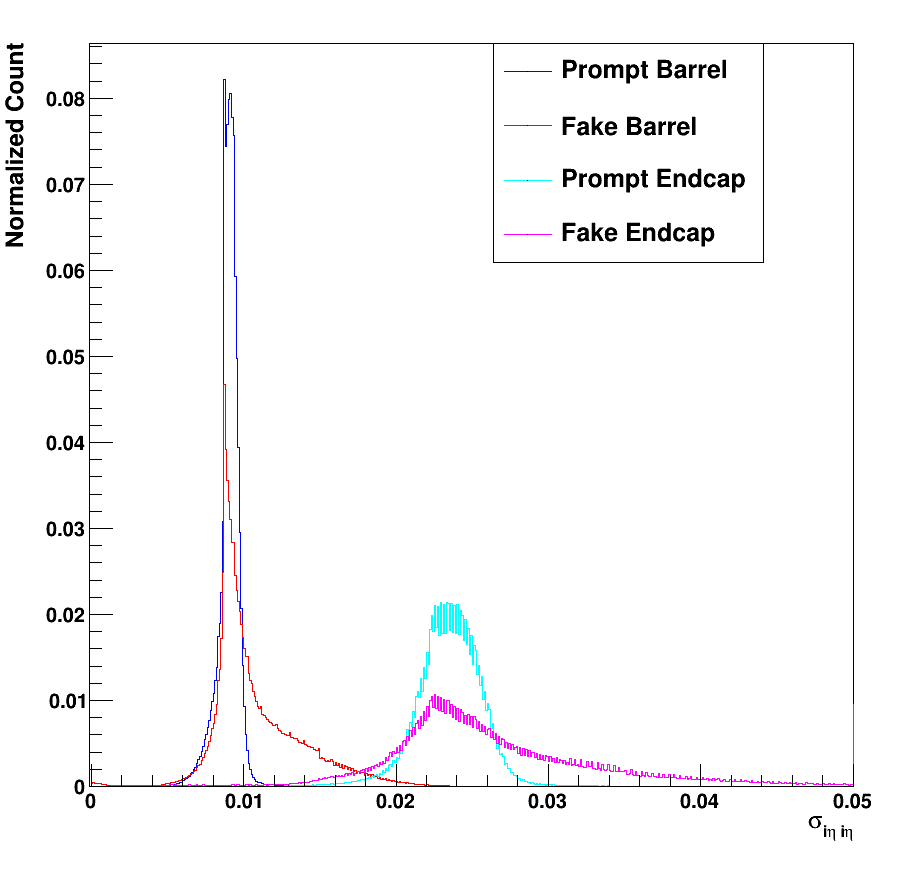
\includegraphics[width=\linewidth]{./Figures/Offline Selection Plots/0709_Updated_GJet_TrainingPlots/sigmaIetaIeta.png}
		\caption{$\sigma_{i \eta i \eta}$}
		\label{GJetVars:sieie}
	\end{subfigure}\hfill
	\begin{subfigure}{0.50\linewidth}
		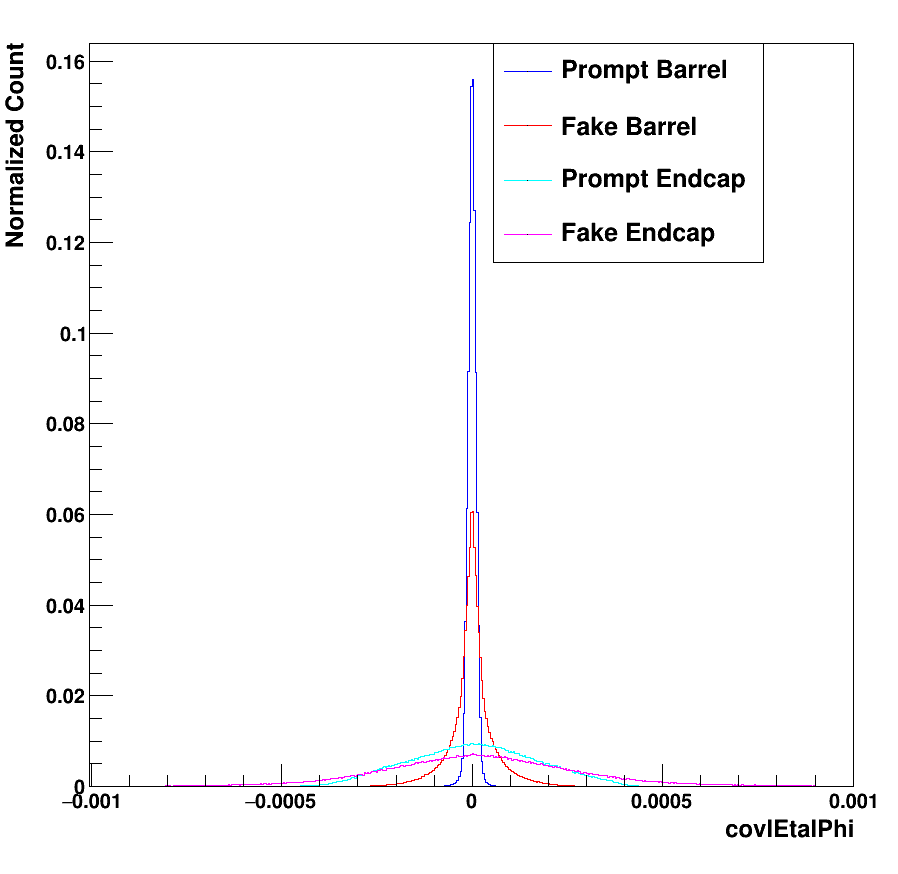
\includegraphics[width=\linewidth]{./Figures/Offline Selection Plots/0709_Updated_GJet_TrainingPlots/covIEtaIPhi.png}
		\caption{cov($i \eta i \phi$)}
		\label{GJetVars:covIetaIphi}
	\end{subfigure}
	\caption{Plots of the $\sigma_{i \eta i \eta}$ and cov($i \eta i \phi$). The prompt signal is shown in dark blue for the barrel and light blue for the endcap, whereas the fake background is shown in red for the barrel and pink for the endcap.}
	\label{fig:GJetVars3}
\end{figure}

Similarly to the $\sigma_{i \eta i \eta}$ and cov($i \eta i \phi$), the $\eta$ and $\phi$ widths are powerful showershape variables that provide some measure of how well-localized the energy deposition is. It is expected that these values are different for the barrel and endcap, as the crystal size and spacing are different in the two different regions of the detector. This can be seen in both plots in figure \ref{fig:GJetVars4}. Additionally, the separation between prompt and fake photons can be clearly seen, especially in $\eta$ width.

\begin{figure}[H]
	\begin{subfigure}{0.50\linewidth}
		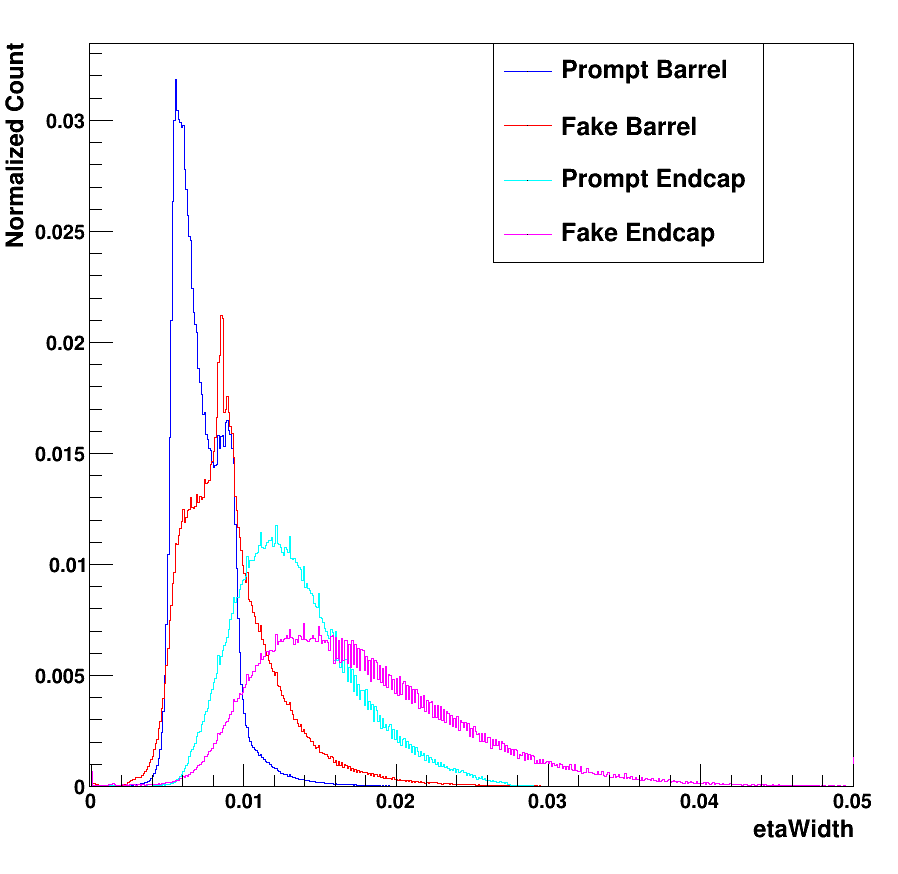
\includegraphics[width=\linewidth]{./Figures/Offline Selection Plots/0709_Updated_GJet_TrainingPlots/etaWidth.png}
		\caption{$\eta$ Width}
		\label{GJetVars:etaW}
	\end{subfigure}\hfill
	\begin{subfigure}{0.50\linewidth}
		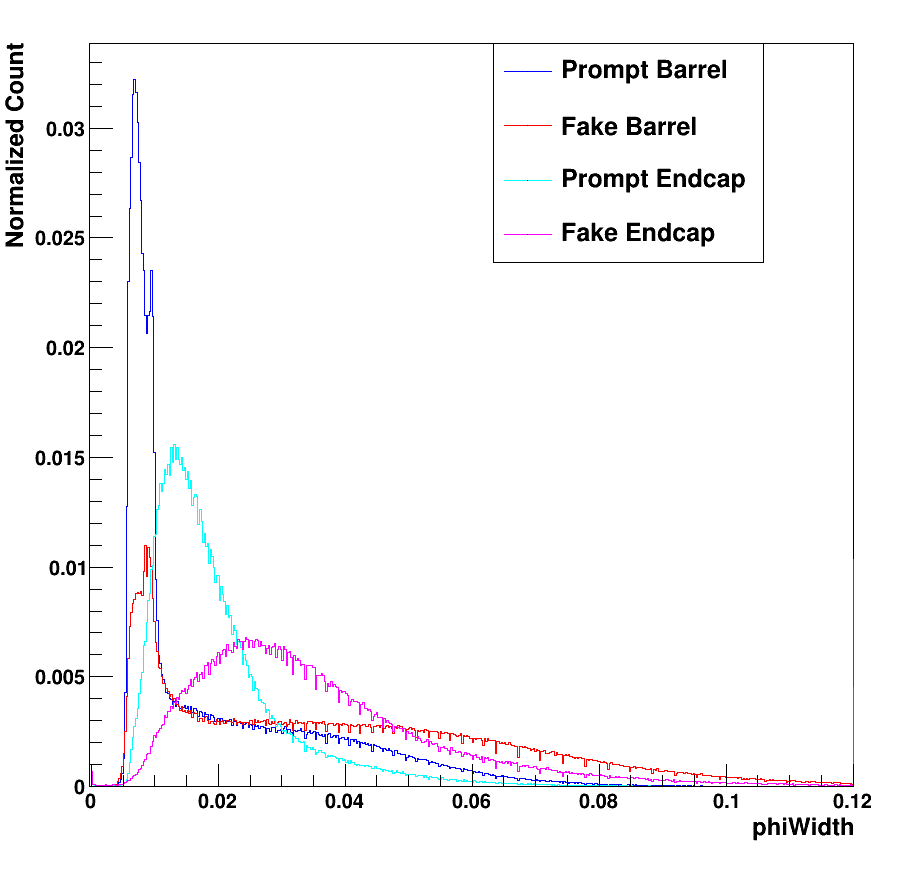
\includegraphics[width=\linewidth]{./Figures/Offline Selection Plots/0709_Updated_GJet_TrainingPlots/phiWidth.png}
		\caption{$\phi$ Width}
		\label{GJetVars:phiW}
	\end{subfigure}
	\caption{Plots of the $\eta$ and $\phi$ widths. The prompt signal is shown in dark blue for the barrel and light blue for the endcap, whereas the fake background is shown in red for the barrel and pink for the endcap.}
	\label{fig:GJetVars4}
\end{figure}

The measure of the HCal energy vs the ECal energy, H/E, provides a powerful measure of whether the energy deposition more closely matches an electromagnetic process -- such as a photon or electron -- or a hadronic process such as a jet. It is expected that most photons will have a value consistent with 0, as they should deposit all of their energy into the ECal. There is, of course, some level of energy leakage that ensures that even photons often do not have an H/E of identically 0. Clearly, however, the prompt photons in both the barrel and endcap strongly peak near 0 and fall off rather quickly below this. Note that figure \ref{sub@GJetVars:hoe} is a log plot, so that the secondary peak below 0 is down by more than a factor of 10 relative to the primary peak at 0. Since the fake photons are jet signatures designed to mimic a prompt signature, they still exhibit a strong peak near 0. It can be seen, however, that the distribution extends to much higher values of H/E overall.  

\begin{figure}[H]
	\begin{subfigure}{0.50\linewidth}
		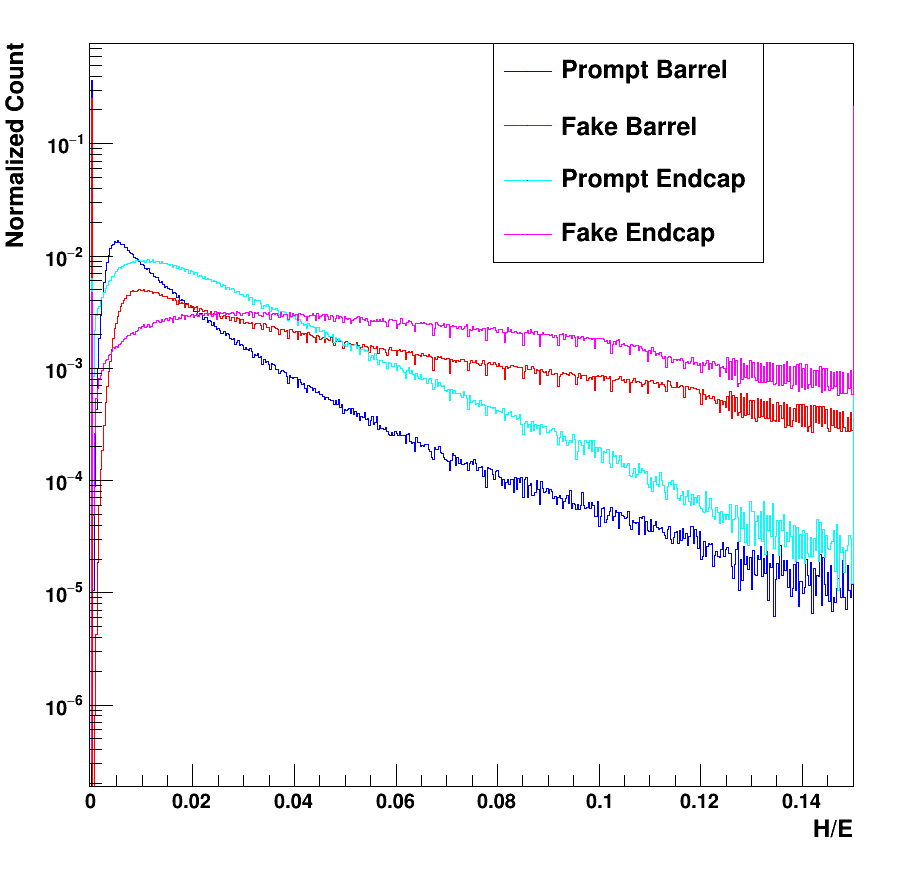
\includegraphics[width=\linewidth]{./Figures/Offline Selection Plots/0709_Updated_GJet_TrainingPlots/hadronicOverEm.png}
		\caption{H/E}
		\label{GJetVars:hoe}
	\end{subfigure}\hfill
	\begin{subfigure}{0.50\linewidth}
		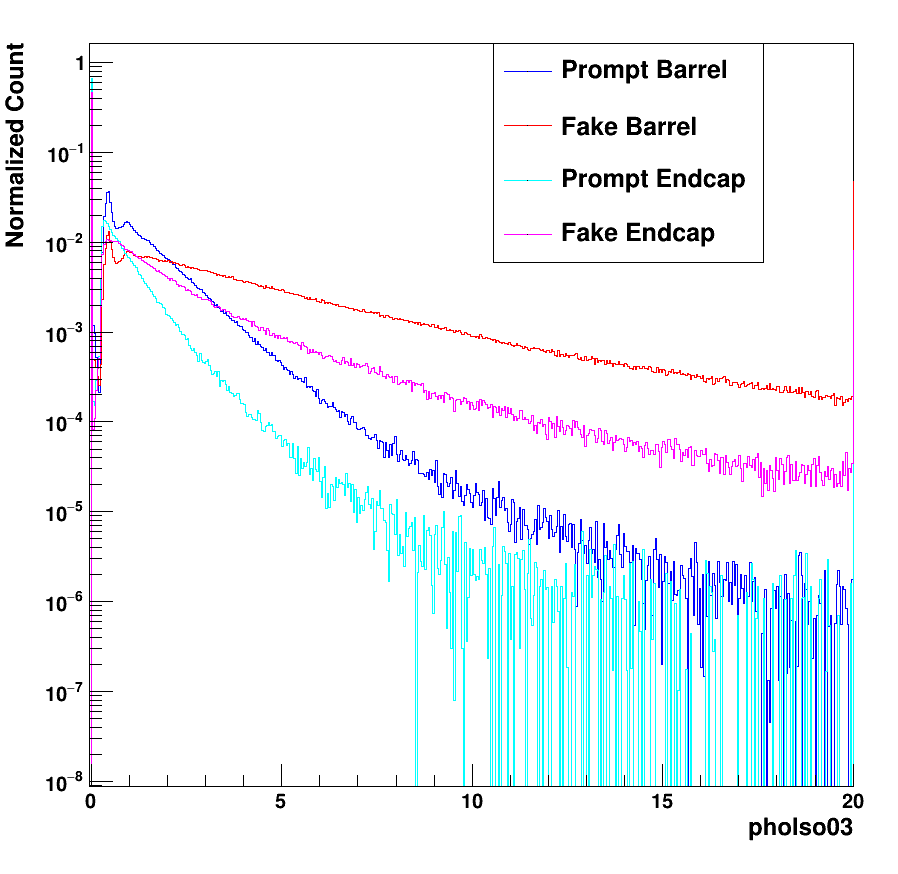
\includegraphics[width=\linewidth]{./Figures/Offline Selection Plots/0709_Updated_GJet_TrainingPlots/phoIso03.png}
		\caption{Photon Isolation}
		\label{GJetVars:phoIso}
	\end{subfigure}
	\caption{Plots of the H/E and photon isolation. The prompt signal is shown in dark blue for the barrel and light blue for the endcap, whereas the fake background is shown in red for the barrel and pink for the endcap.}
	\label{fig:GJetVars5}
\end{figure}

The charge isolation variables are the next input variables, and represent the isolation energy (in GeV) relative to a specific vertex. The vertexing described in section \ref{sec:OfflineReco} provides multiple vertices at the NanoAOD level. Isolations are measured relative to both the worst possible vertex (figure \ref{GJetVars:chgIsoWorst}), and the final chosen vertex (figure \ref{GJetVars:chgIsoChosen}). While the chosen vertex often has 0 isolation energy, the worst vertex very rarely does. In both cases, however, the separation between signal and background is clear for both the barrel and endcap. The charge isolation w.r.t. worst vertex, specifically, shows very clear and powerful spearation.

\begin{figure}[H]
	\begin{subfigure}{0.50\linewidth}
		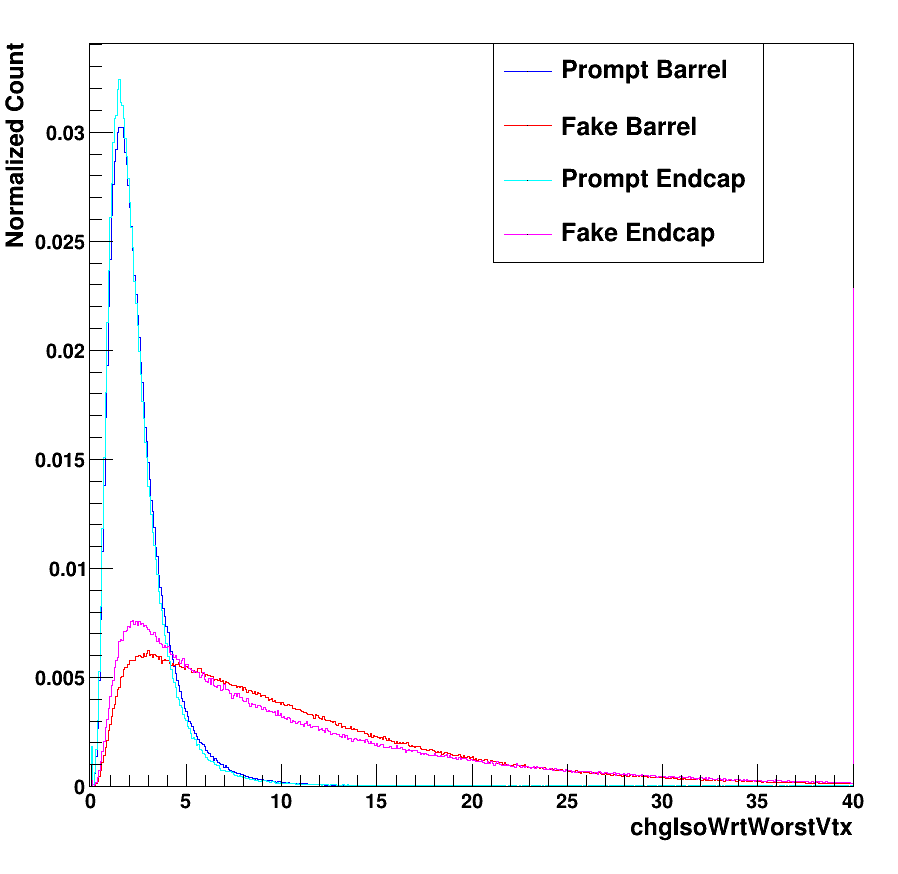
\includegraphics[width=\linewidth]{./Figures/Offline Selection Plots/0709_Updated_GJet_TrainingPlots/chgIsoWrtWorstVtx.png}
		\caption{Chg. Iso. W.r.t. Worst Vertex}
		\label{GJetVars:chgIsoWorst}
	\end{subfigure}\hfill
	\begin{subfigure}{0.50\linewidth}
		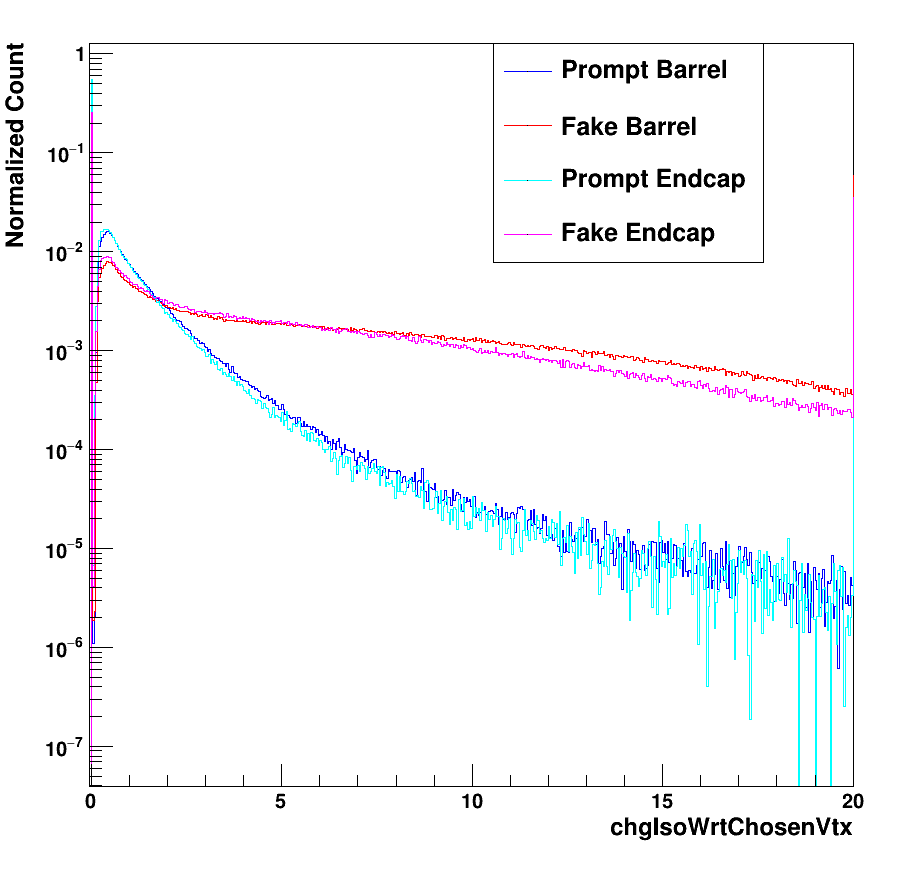
\includegraphics[width=\linewidth]{./Figures/Offline Selection Plots/0709_Updated_GJet_TrainingPlots/chgIsoWrtChosenVtx.png}
		\caption{Chg. Iso. W.r.t. Chosen Vertex}
		\label{GJetVars:chgIsoChosen}
	\end{subfigure}
	\caption{Plots of the charged isolations with respect to the chosen and worst vertices. The prompt signal is shown in dark blue for the barrel and light blue for the endcap, whereas the fake background is shown in red for the barrel and pink for the endcap.}
	\label{fig:GJetVars6}
\end{figure}

The final two variables in the model are only used in the endcap models. In fact, these variables only exist for endcap events.

\begin{figure}[H]
	\begin{subfigure}{0.50\linewidth}
		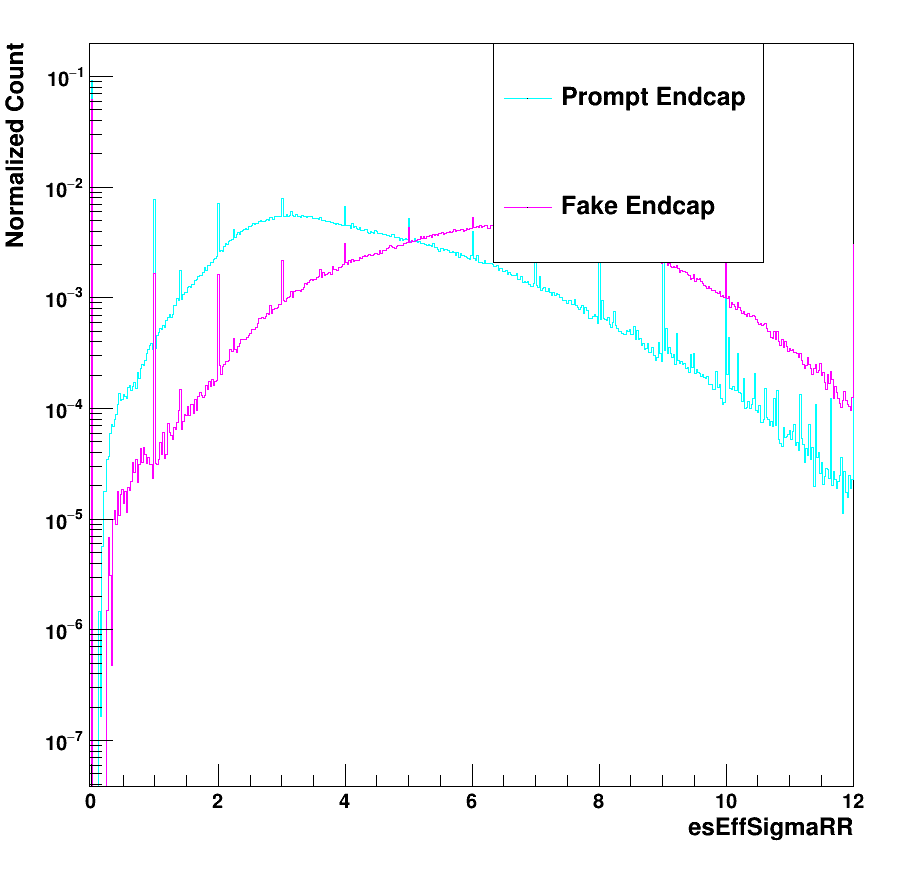
\includegraphics[width=\linewidth]{./Figures/Offline Selection Plots/0709_Updated_GJet_TrainingPlots/esEffSigmaRR.png}
		\caption{ES Eff. Sigma RR}
		\label{GJetVars:esEffSigmaRR}
	\end{subfigure}\hfill
	\begin{subfigure}{0.50\linewidth}
		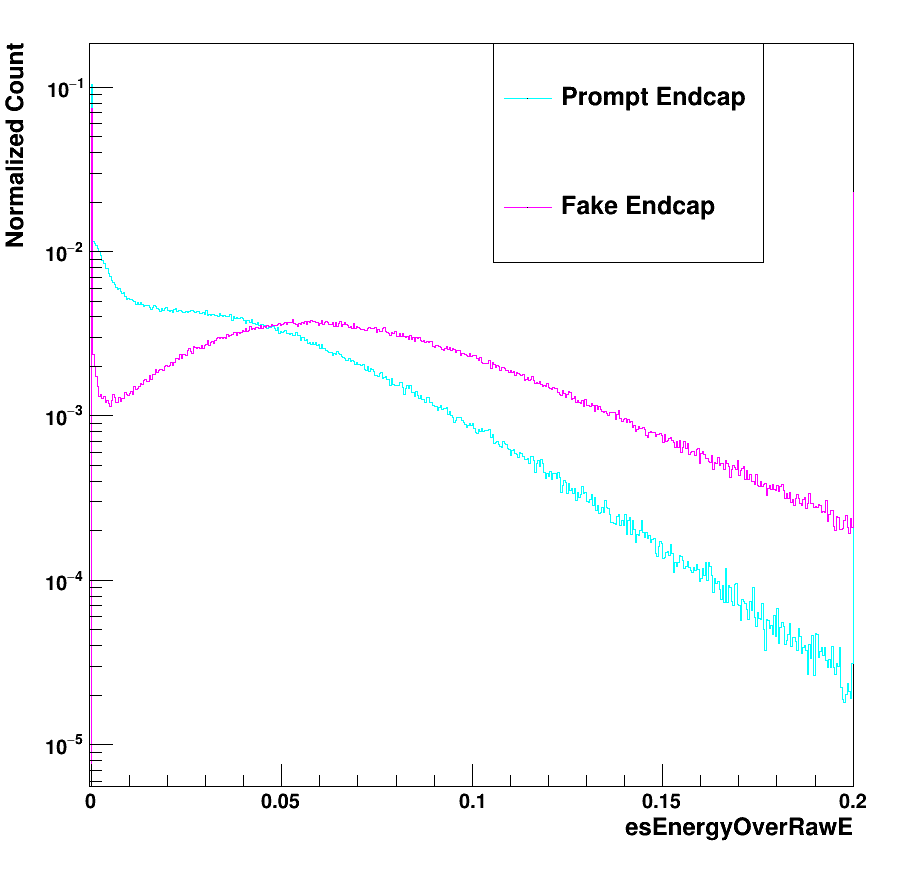
\includegraphics[width=\linewidth]{./Figures/Offline Selection Plots/0709_Updated_GJet_TrainingPlots/esEnergyOverRawE.png}
		\caption{ES Energy over Raw E}
		\label{GJetVars:esEnergyOverRawE}
	\end{subfigure}
	\caption{Plots of two endcap-specific variables: esEffSigmaRR and esEnergyOverRawE. The prompt signal is shown in light blue, whereas the fake background is shown in pink.}
	\label{fig:GJetVars7}
\end{figure}

Comparing to the MVA-HLT variables shown in \ref{tab:HLTInputVars}, it can be seen that a few variables have been added at the offline selection level. The photon isolation is analogous to the ECalIso used at the trigger level, but is calculated differently (how?). The two charged isolations used are entirely new additions, as the MVA-HLT is calculated before any complex vertexing is implemented. (Why are both used?). (Statements on rho, and the endcap variables)

The hyperparameter optimization at the offline level was performed very similarly to the MVA-HLT; the max depth and learning rate were varied in tandem until an optimal point was found. The same process of early stopping within XGBoost was used, as well. The hyperparameters were, however, found to be quite different from the trigger-level optimization. Since there are considerably more input variables used (13/15 for the barrel/endcap versus the 8 for the trigger), the max depth was necessarily higher. Consequently, the learning rate was also made lower. The optimum hyperparameters were, then, found to be a maximum depth of 18 and a learning rate of 0.06. 

\subsubsection{A Data/MC BDT for $H \rightarrow \gamma \gamma$}
While the above $\gamma + Jet$ BDT can help differentiate real photon candidates from fakes, it cannot, in principle, properly differentiate a photon candidate coming from a signal process from a photon candidate coming from a background process. Since the EGamma trigger selections will already cut out many events with jet-like photon candidates, much of the $H \rightarrow \gamma \gamma$ preselection is aimed at removing real photons coming from non-resonant processes (or even non-Higgs resonances). For the standard preselection, the $p_T$ and $p_T/M_{\gamma \gamma}$ cuts achieve this.  

Furthermore, the $\gamma + Jet$ BDT does not properly mirror the MVA-HLT; since the trigger-level BDT was training using Higgs MC as the signal and real data as the background, the offline selection should employ a similar strategy. So, in the same way that the trigger was trained using signal photon candidates originating from a ggH MC sample and background photon candidates originating from the data. The same input variables used in the $\gamma + Jet$ BDT were then used to train and optimimize the new model. These input variables are plotted in the same way as for the previous section, with the barrel and endcap signal being shown in dark and light blue, respectively. Meanwhile, the barrel and endcap background will be shown in red and pink. 

\begin{figure}[H]
	\begin{subfigure}{0.50\linewidth}
		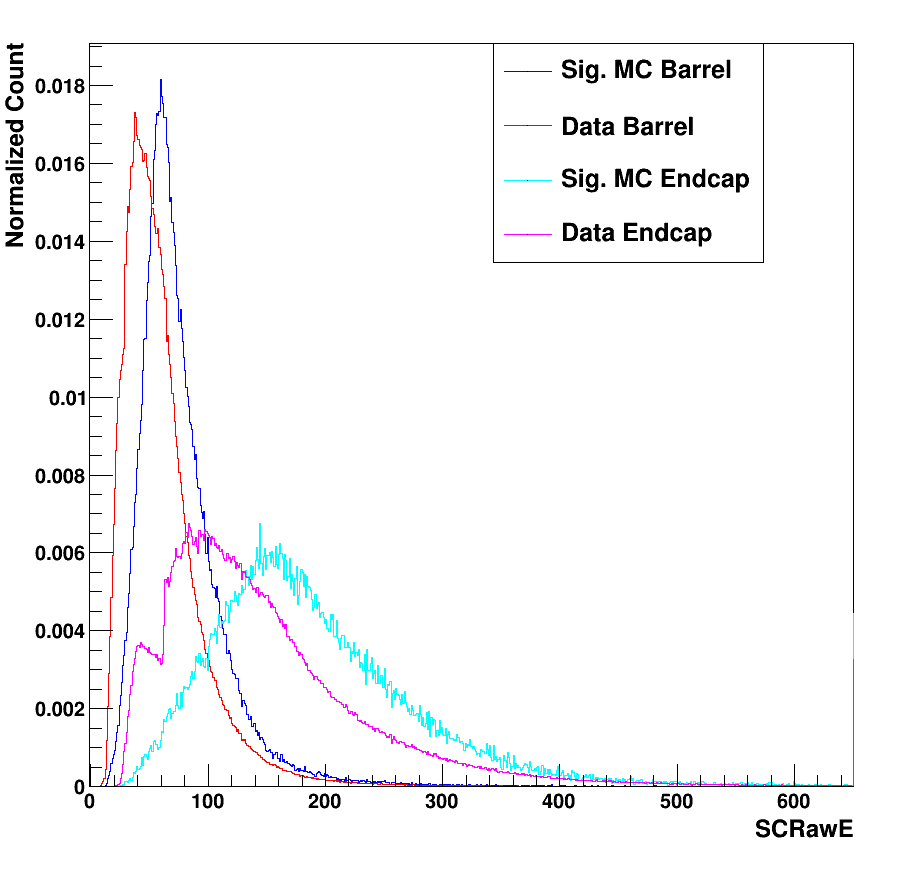
\includegraphics[width=\linewidth]{./Figures/Offline Selection Plots/0709_Updated_DataMC_TrainingPlots/SCRawE.png}
		\caption{Raw Energy}
		\label{DataMCVars:RawE}
	\end{subfigure}\hfill
	\begin{subfigure}{0.50\linewidth}
		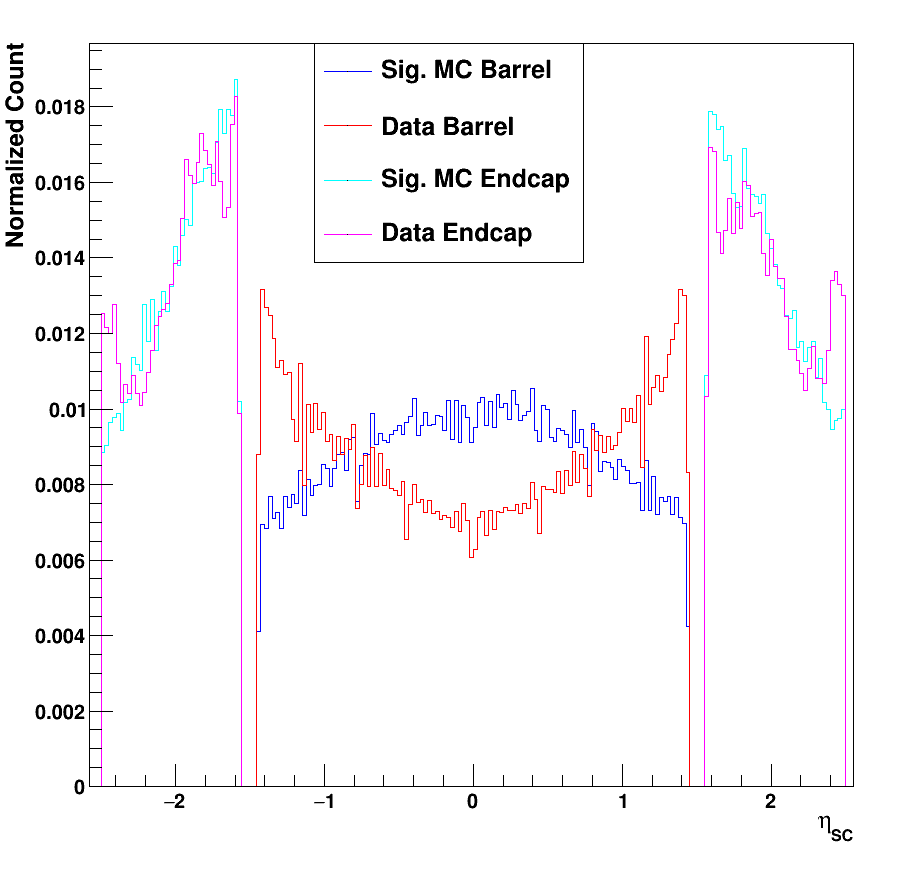
\includegraphics[width=\linewidth]{./Figures/Offline Selection Plots/0709_Updated_DataMC_TrainingPlots/scEta.png}
		\caption{$\eta_{SC}$}
		\label{DataMCVars:eta}
	\end{subfigure}
	\caption{Plots of the Supercluster raw energy and $\eta{SC}$. The prompt signal is shown in dark blue for the barrel and light blue for the endcap, whereas the fake background is shown in red for the barrel and pink for the endcap.}
	\label{fig:DataMCVars1}
\end{figure}

Similarly to the $\gamma$ + Jet distributions, a clear difference can be seen in \ref{DataMCVars:RawE} between the barrel and endcap distributions of the signal and background. In contrast, however, the difference between signal and background is less pronounced for the data and signal MC. As a result, this will be a less powerful discrimination variable for this new BDT. The features of the $\eta_{SC}$ distributions for the data and MC differ considerably more than those for the $\gamma$ + Jet prompt and fake distributions, however. Particularly in the barrel, it can be seen that the signal MC tends to be much more centeral, whereas the data peaks strongly towards to high-$\eta$ regions of the barrel. The endcap distributions, however, are much more similar than they were for the $\gamma$ + Jet.

\begin{figure}[H]
	\begin{subfigure}{0.50\linewidth}
		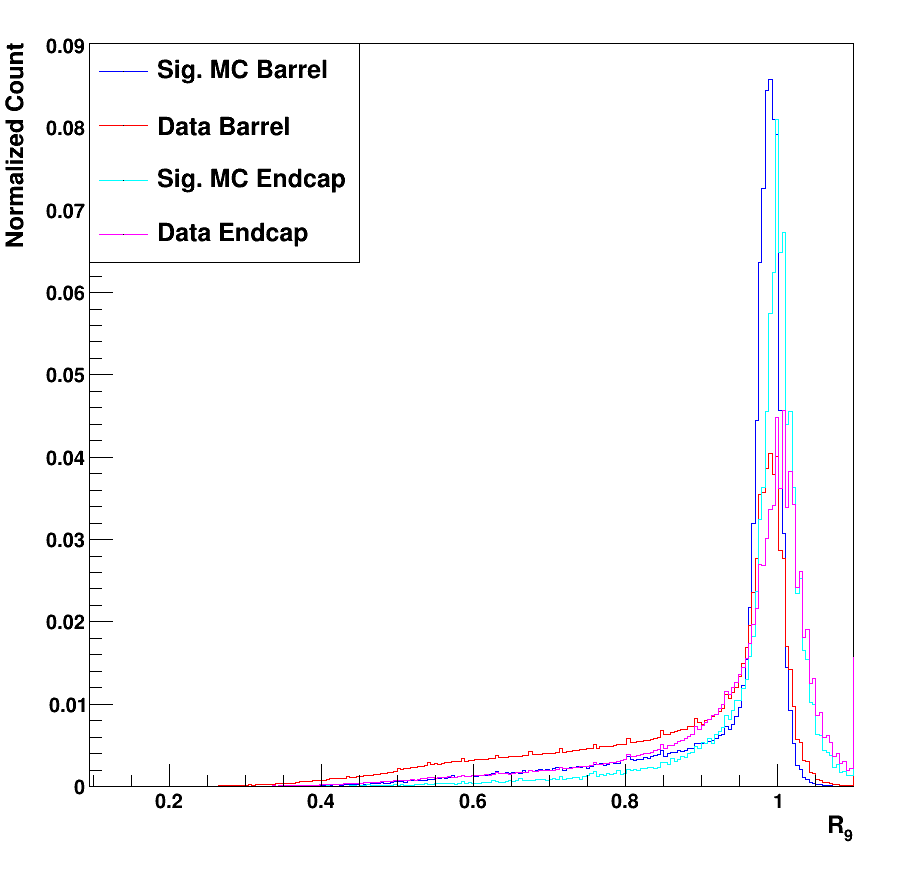
\includegraphics[width=\linewidth]{./Figures/Offline Selection Plots/0709_Updated_DataMC_TrainingPlots/r9.png}
		\caption{$R_9$}
		\label{DataMCVars:r9}
	\end{subfigure}\hfill
	\begin{subfigure}{0.50\linewidth}
		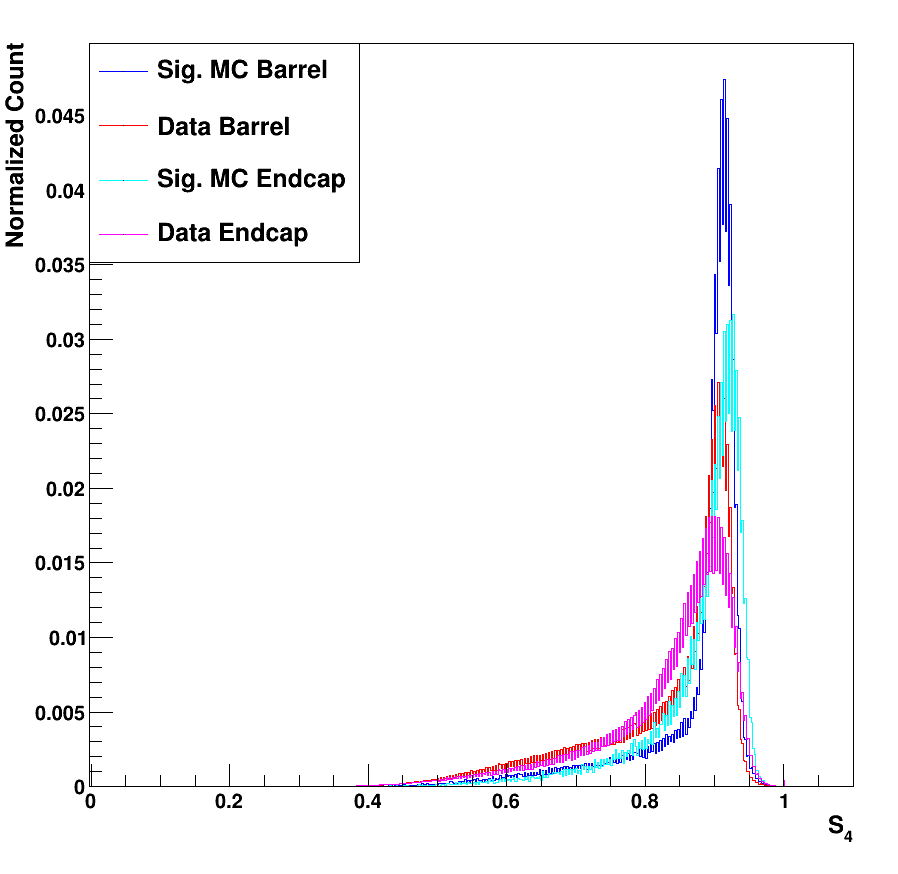
\includegraphics[width=\linewidth]{./Figures/Offline Selection Plots/0709_Updated_DataMC_TrainingPlots/s4.png}
		\caption{$S_4$}
		\label{DataMCVars:s4}
	\end{subfigure}
	\caption{Plots of the $R_9$ and $S_4$. The prompt signal is shown in dark blue for the barrel and light blue for the endcap, whereas the fake background is shown in red for the barrel and pink for the endcap.}
	\label{fig:DataMCVars2}
\end{figure}

As with the $\gamma$ + Jet distributions, the $R_9$ (figure \ref{DataMCVars:r9}) and $S_4$ (figure \ref{DataMCVars:s4}) variables for the signal tend to be much more strongly peaked near 1 compared to the background.

\begin{figure}[H]
	\begin{subfigure}{0.50\linewidth}
		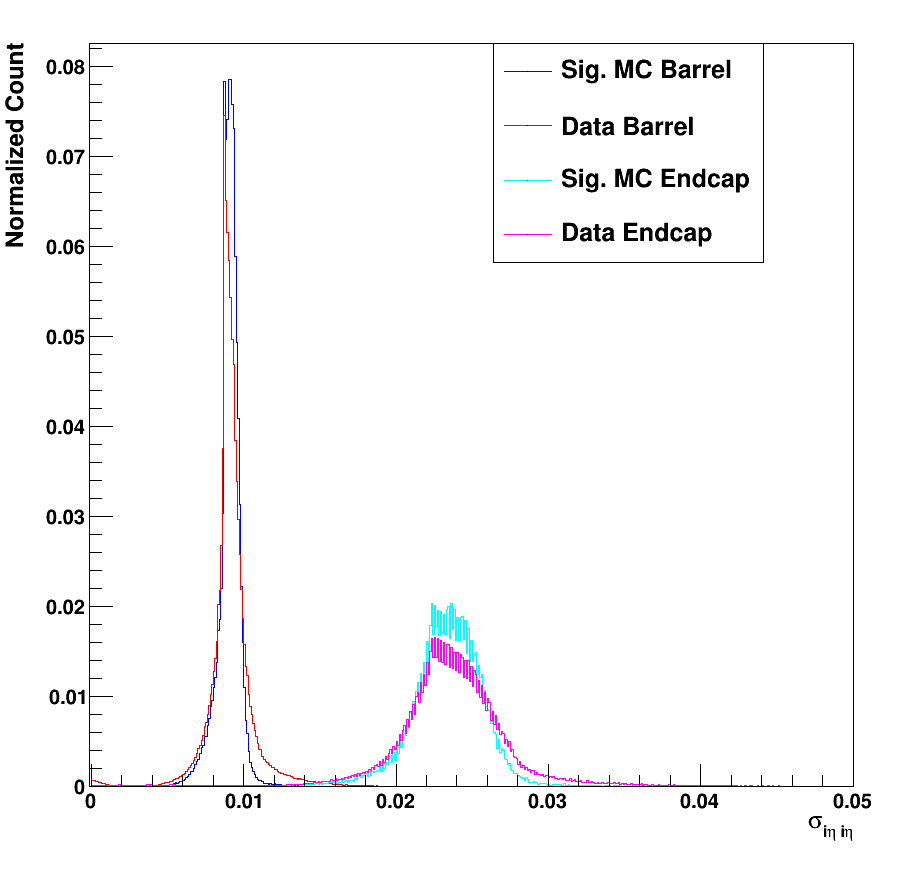
\includegraphics[width=\linewidth]{./Figures/Offline Selection Plots/0709_Updated_DataMC_TrainingPlots/sigmaIetaIeta.png}
		\caption{$\sigma_{i \eta i \eta}$}
		\label{DataMCVars:sieie}
	\end{subfigure}\hfill
	\begin{subfigure}{0.50\linewidth}
		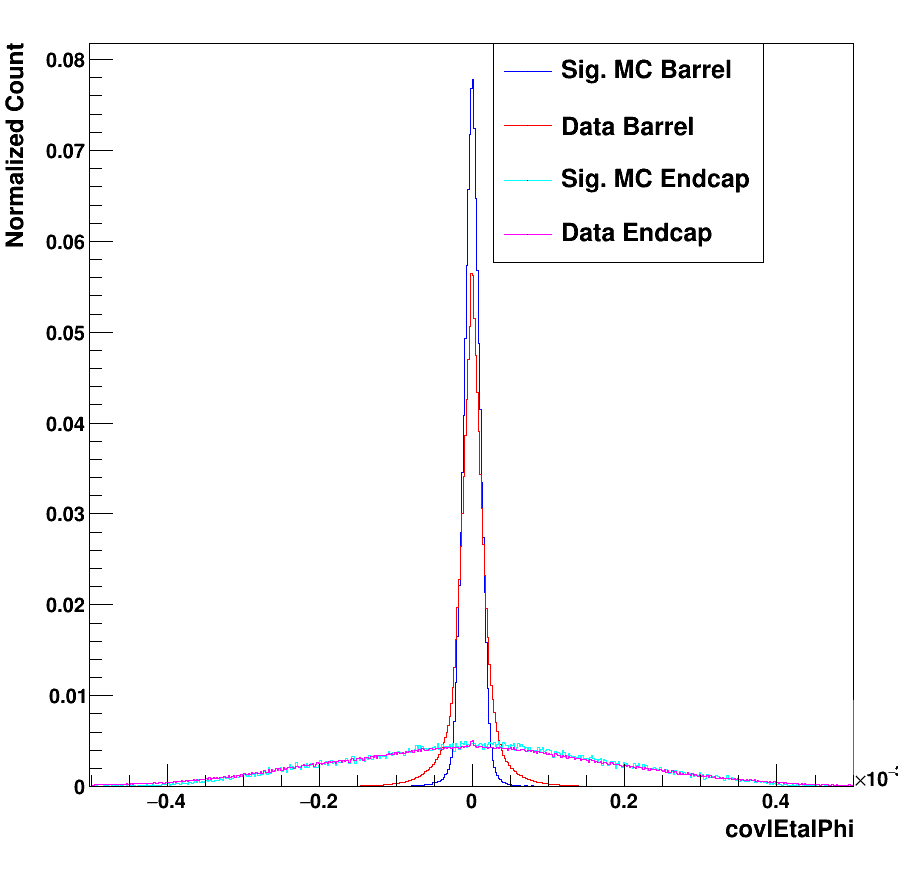
\includegraphics[width=\linewidth]{./Figures/Offline Selection Plots/0709_Updated_DataMC_TrainingPlots/covIEtaIPhi.png}
		\caption{cov($i \eta i \phi$)}
		\label{DataMCVars:covIetaIphi}
	\end{subfigure}
	\caption{Plots of the $\sigma_{i \eta i \eta}$ and cov($i \eta i \phi$). The prompt signal is shown in dark blue for the barrel and light blue for the endcap, whereas the fake background is shown in red for the barrel and pink for the endcap.}
	\label{fig:DataMCVars3}
\end{figure}

In figure \ref{fig:DataMCVars3}, it can be seen that the signal and background distributions are quite similar for both $\sigma_{i \eta i \eta}$ and cov($i \eta i \phi$). Compared to the $\gamma$ + Jet BDT, this means that these showershape variables will be much less powerful. Likely, due to the MVA-HLT selection applied, many of the more jet-like photons have already been removed from this training sample.

\begin{figure}[H]
	\begin{subfigure}{0.50\linewidth}
		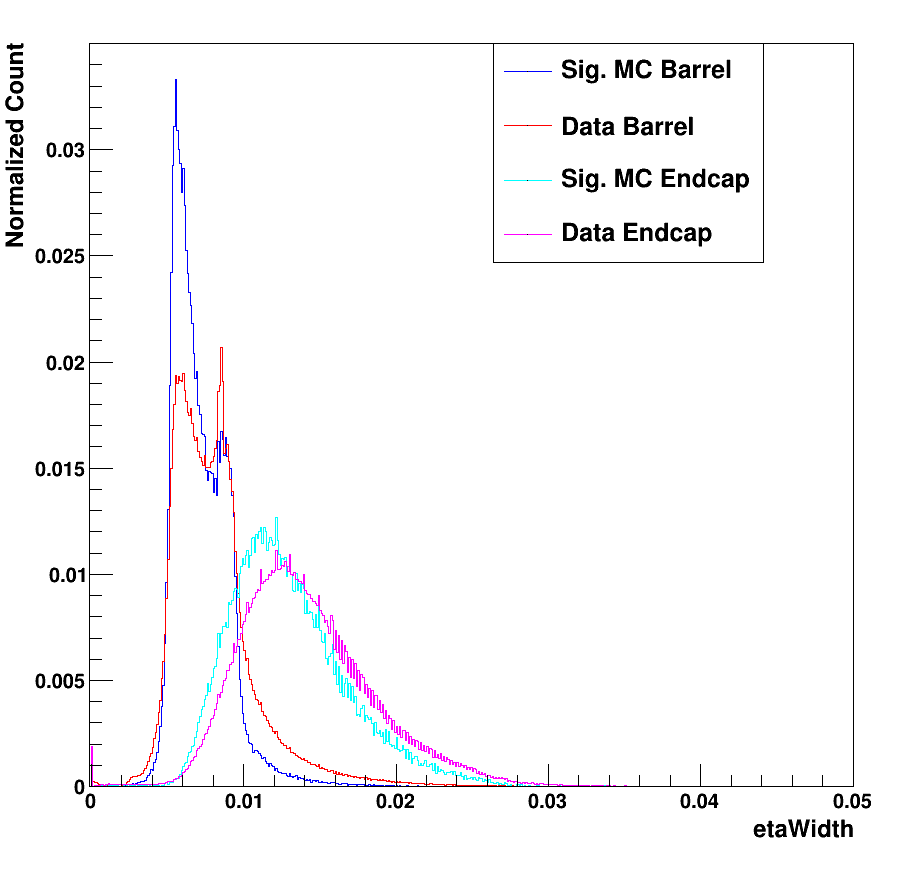
\includegraphics[width=\linewidth]{./Figures/Offline Selection Plots/0709_Updated_DataMC_TrainingPlots/etaWidth.png}
		\caption{$\eta$ Width}
		\label{DataMCVars:etaW}
	\end{subfigure}\hfill
	\begin{subfigure}{0.50\linewidth}
		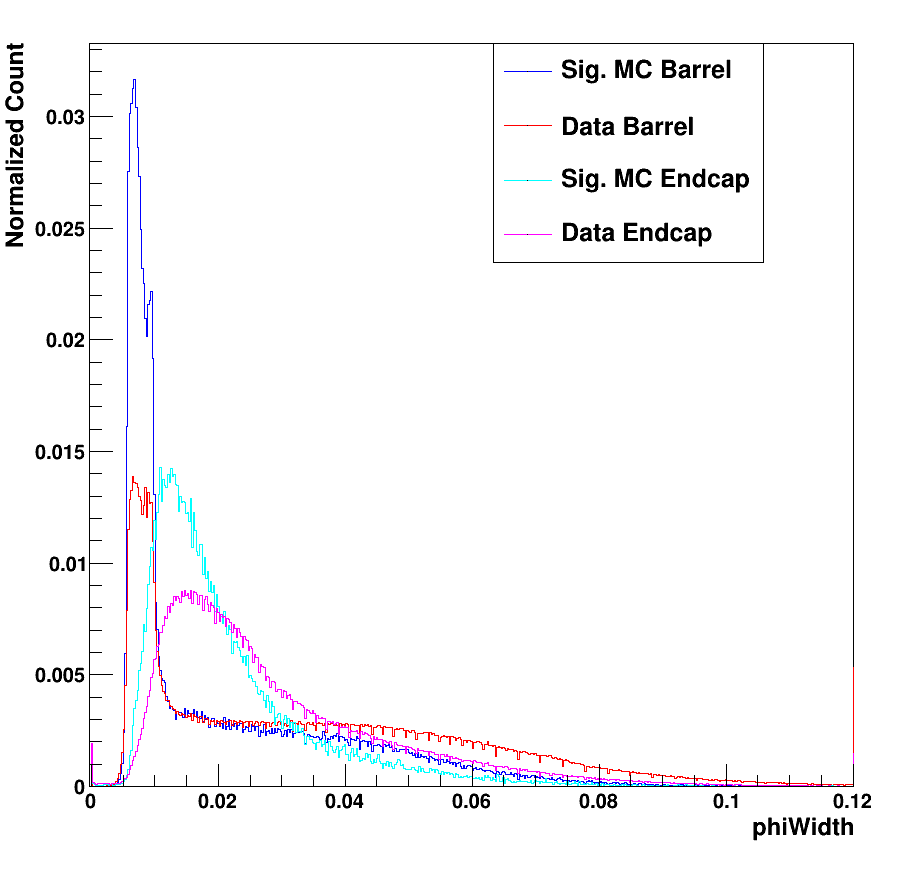
\includegraphics[width=\linewidth]{./Figures/Offline Selection Plots/0709_Updated_DataMC_TrainingPlots/phiWidth.png}
		\caption{$\phi$ Width}
		\label{DataMCVars:phiW}
	\end{subfigure}
	\caption{Plots of the $\eta$ and $\phi$ widths. The prompt signal is shown in dark blue for the barrel and light blue for the endcap, whereas the fake background is shown in red for the barrel and pink for the endcap.}
	\label{fig:DataMCVars4}
\end{figure}

The $\eta$ and $\phi$ widths in figure \ref{fig:DataMCVars4} show similar separation between signal and background relative to the $\gamma$ + Jet distributions. 

\begin{figure}[H]
	\begin{subfigure}{0.50\linewidth}
		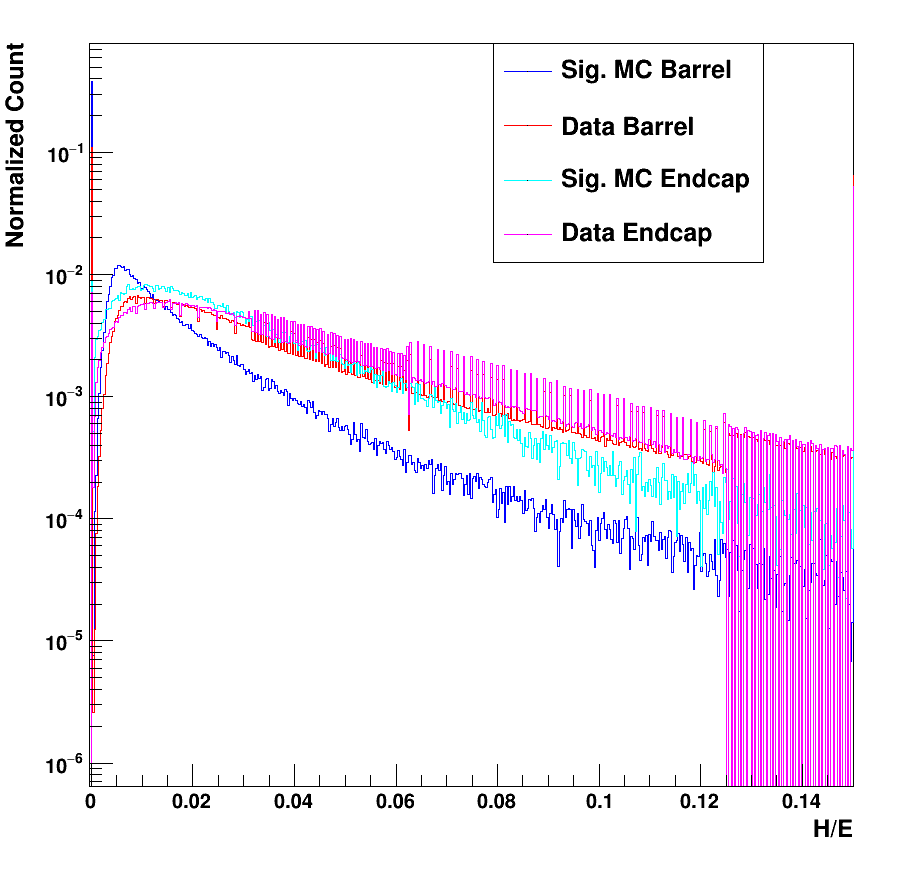
\includegraphics[width=\linewidth]{./Figures/Offline Selection Plots/0709_Updated_DataMC_TrainingPlots/hadronicOverEm.png}
		\caption{H/E}
		\label{DataMCVars:hoe}
	\end{subfigure}\hfill
	\begin{subfigure}{0.50\linewidth}
		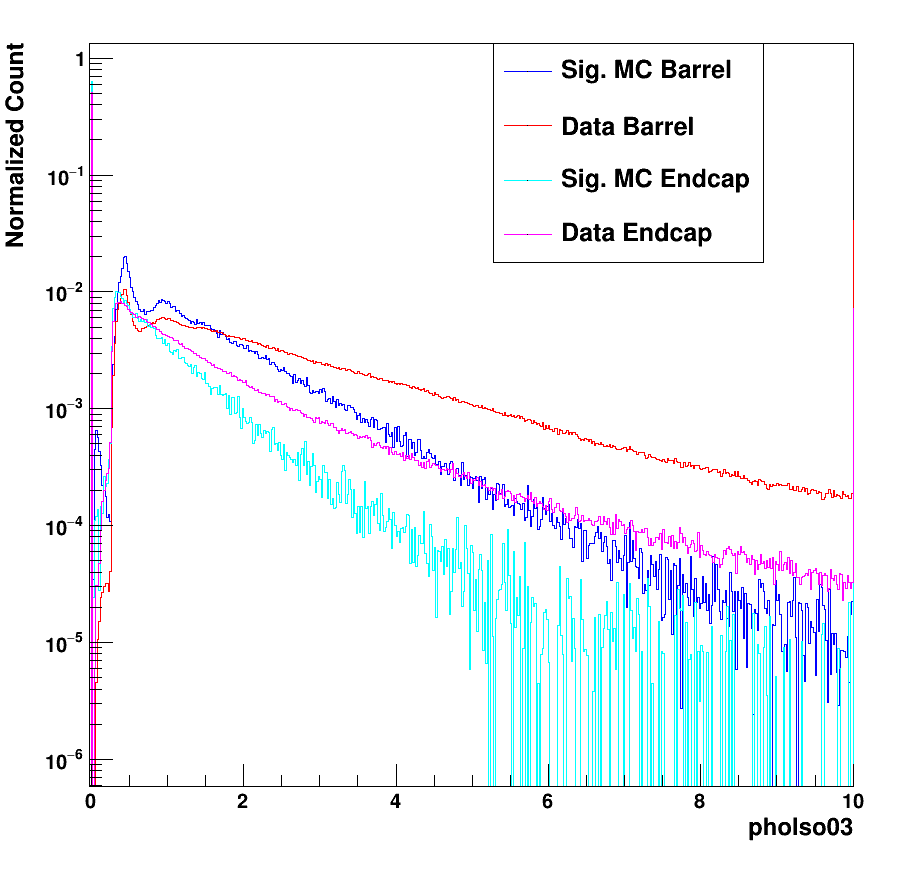
\includegraphics[width=\linewidth]{./Figures/Offline Selection Plots/0709_Updated_DataMC_TrainingPlots/phoIso03.png}
		\caption{Photon Isolation}
		\label{DataMCVars:phoIso}
	\end{subfigure}
	\caption{Plots of the H/E and photon isolation. The prompt signal is shown in dark blue for the barrel and light blue for the endcap, whereas the fake background is shown in red for the barrel and pink for the endcap.}
	\label{fig:DataMCVars5}
\end{figure}

The H/E and photon isolation in figure \ref{fig:DataMCVars5} show decent separation between the signal MC and data in both the barrel and endcap. The barrel and endcap for the data are quite similar for H/E, while the signal MC shows considerably more variation between the two detector elements. Overall, H/E remains a quite powerful discrimination variable in these new samples. Similarly, clear differences can be seen between the signal and background in the photon isolation.

\begin{figure}[H]
	\begin{subfigure}{0.50\linewidth}
		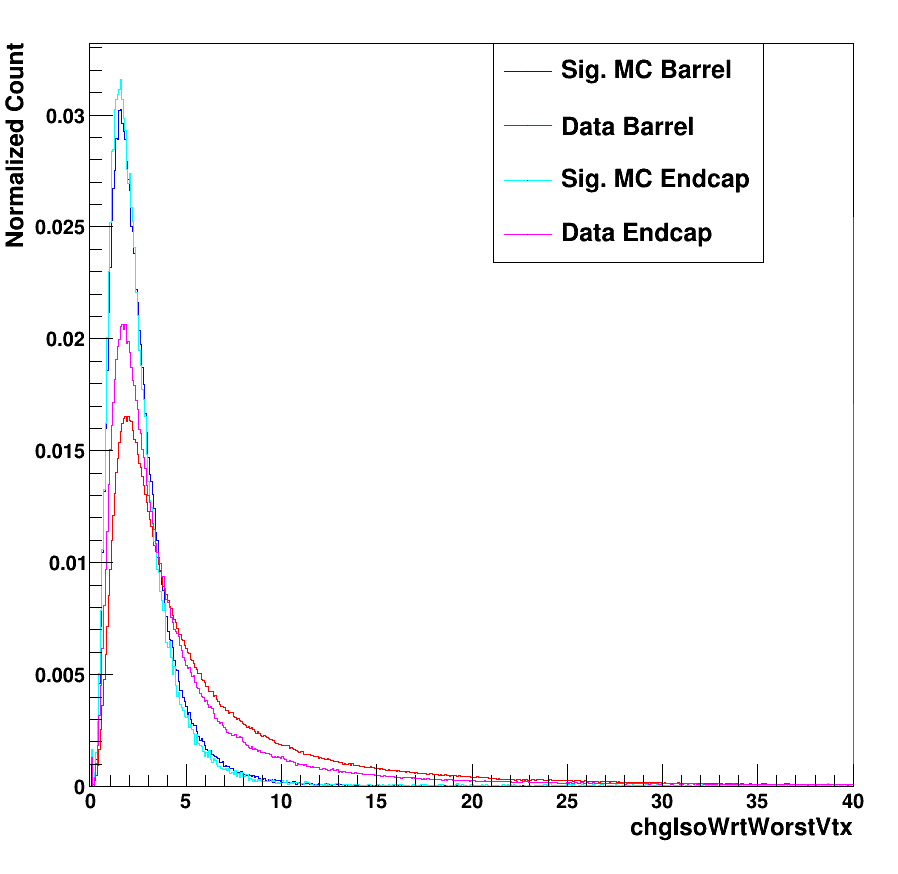
\includegraphics[width=\linewidth]{./Figures/Offline Selection Plots/0709_Updated_DataMC_TrainingPlots/chgIsoWrtWorstVtx.png}
		\caption{Chg. Iso. W.r.t. Worst Vertex}
		\label{DataMCVars:chgIsoWorst}
	\end{subfigure}\hfill
	\begin{subfigure}{0.50\linewidth}
		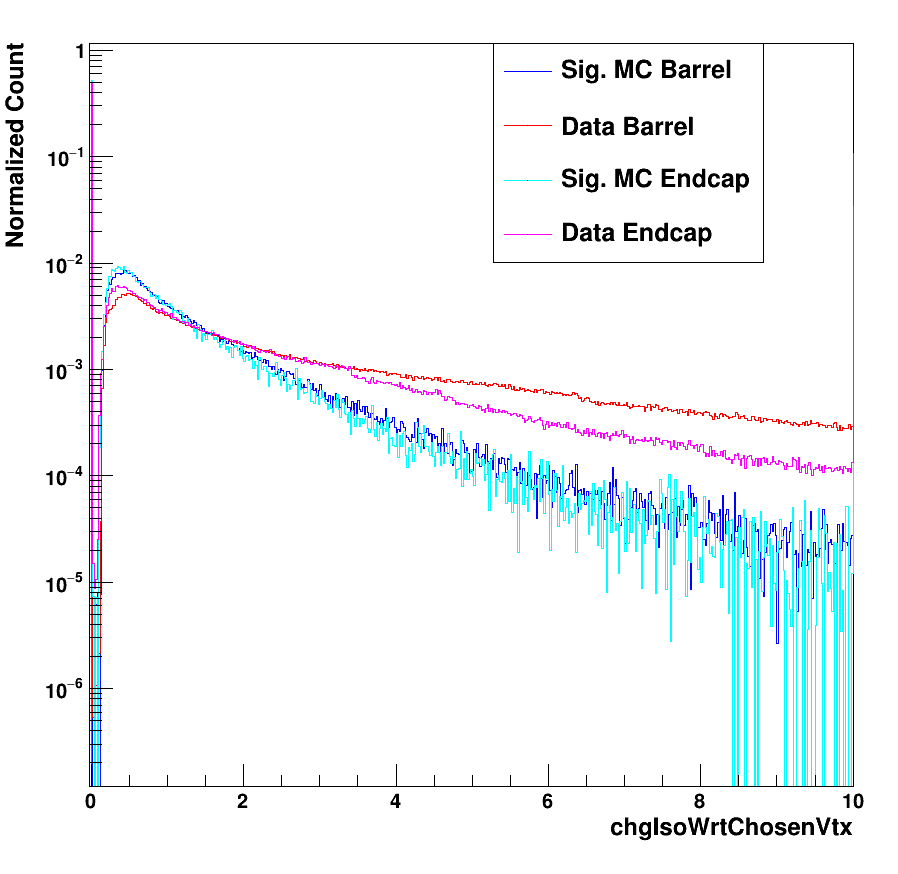
\includegraphics[width=\linewidth]{./Figures/Offline Selection Plots/0709_Updated_DataMC_TrainingPlots/chgIsoWrtChosenVtx.png}
		\caption{Chg. Iso. W.r.t. Chosen Vertex}
		\label{DataMCVars:chgIsoChosen}
	\end{subfigure}
	\caption{Plots of the charged isolations with respect to the chosen and worst vertices. The prompt signal is shown in dark blue for the barrel and light blue for the endcap, whereas the fake background is shown in red for the barrel and pink for the endcap.}
	\label{fig:DataMCVars6}
\end{figure}

In figure \ref{fig:DataMCVars6}, it can immediately be seen that the two charge isolations are quite similar for the signal and background in both the barrel and endcap. While the values tend to extend a bit higher for the background overall, the shapes are far more similar between the signal and background classes relative to the $\gamma$ + Jet distributions. 

\begin{figure}[H]
	\begin{subfigure}{0.50\linewidth}
		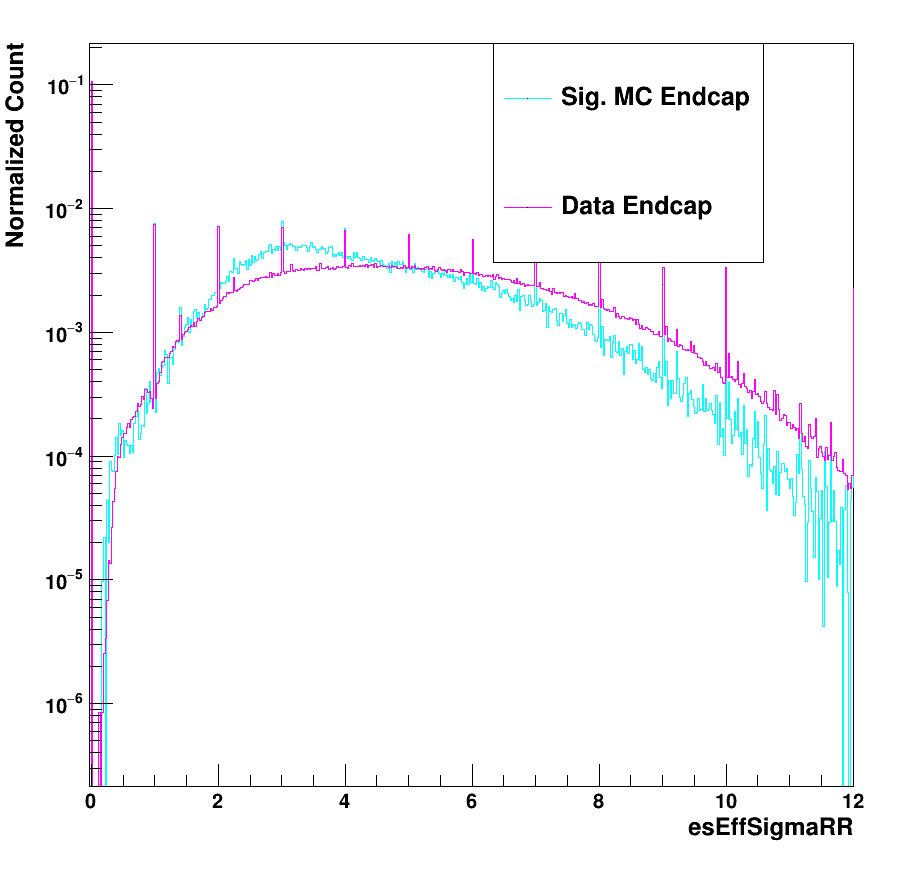
\includegraphics[width=\linewidth]{./Figures/Offline Selection Plots/0709_Updated_DataMC_TrainingPlots/esEffSigmaRR.png}
		\caption{ES Eff. Sigma RR}
		\label{DataMCVars:esEffSigmaRR}
	\end{subfigure}\hfill
	\begin{subfigure}{0.50\linewidth}
		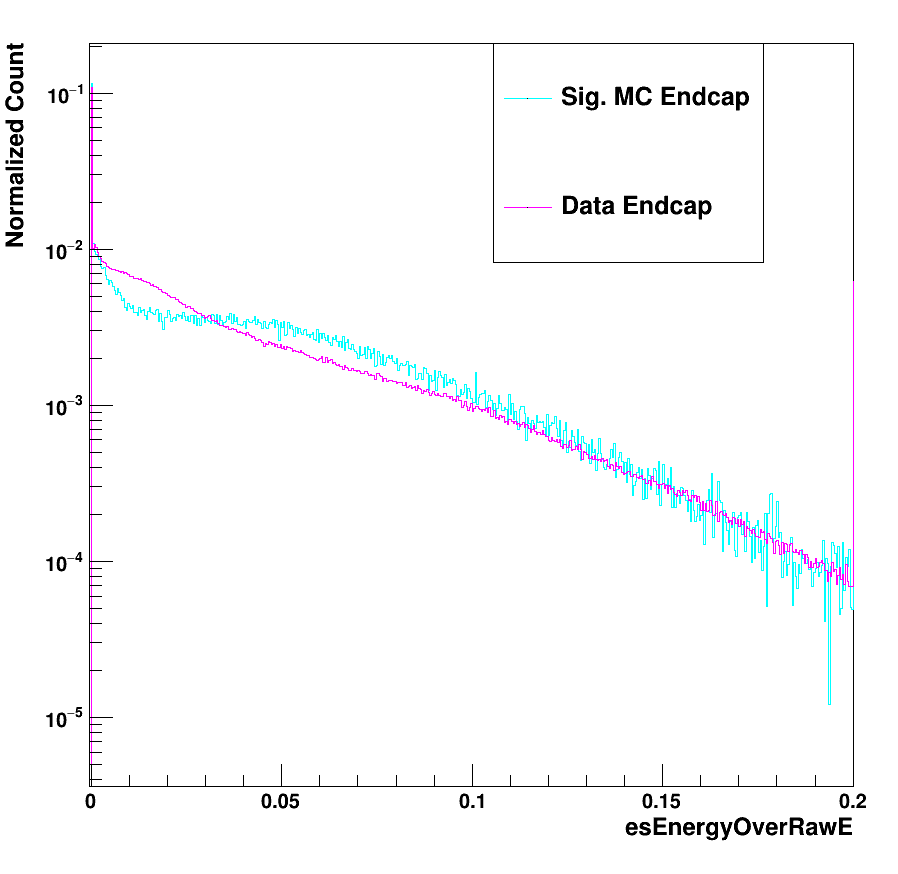
\includegraphics[width=\linewidth]{./Figures/Offline Selection Plots/0709_Updated_DataMC_TrainingPlots/esEnergyOverRawE.png}
		\caption{ES Energy over Raw E}
		\label{DataMCVars:esEnergyOverRawE}
	\end{subfigure}
	\caption{Plots of two endcap-specific variables: esEffSigmaRR and esEnergyOverRawE. The prompt signal is shown in light blue, whereas the fake background is shown in pink.}
	\label{fig:DataMCVars7}
\end{figure}

The same process of hyperparameter optimzation as the previous models was used. Notably, the signal MC and data show much more similarity in the input variable distributions relative to the $\gamma$ + Jet samples. As a result, the model must become a bit more complex to achieve the desired discrimination power. The same experimental optimization process led to a maximum depth of 18 paired with a learning rate of 0.025. While the maximum depth is the same as that of the $\gamma$ + Jet model, the learning rate is quite a bit lower than the 0.06 used for that BDT.
 
\subsection{Determination of Loose Single Photon MVA Cuts for $H \rightarrow \gamma \gamma$} \label{sec:SingleHSinglePhoCuts}
The preexisting preselection first makes decently loose cuts on individual photons, then tighter $p_T$ and $p_T/M_{\gamma \gamma}$ cuts on selected diphoton combinations. A very similar strategy can be used for the BDT-based offline selection. Firstly, loose cuts on the above BDT scores can be applied to the individual photon candidates, which will reduce the number of possible diphoton combinations and cut out many events with no reasonable photon candidates. Then, with the list of individual photons cleaned up a bit, a tighter selection can be applied to the resulting diphoton objects for the selection of a final pair of photons. 

So, then, the aim is to choose a loose set of cuts on the $\gamma + Jet$ and Data/MC BDT scores before applying a tighter final selection on the resulting diphoton combinations. One great advantage of a BDT-based approach is the ease with which these cuts can be adjusted and optimized; while a many-variable preselection has several different cuts to optimize, a binary classifier BDT only has a single output score on which to make cuts. While the goal of this current offline selection is to demonstrate an example analysis that leverages the increased signal efficiency of the MVA-HLT, the existence of these single photon scores allows very easy tuning of the photon preselection for any given analysis. The example cuts chosen below were designed to reduce the signal efficiency by about 2\%, which primarily serves to reduce the number of possible photon combinations for final selection; ultimately, the diphoton cuts described in \ref{sec:DiphotonBDT} will be the primary final selection used to achieve the desired data rate. 

\begin{figure}[H]
	\begin{subfigure}{0.50\linewidth}
		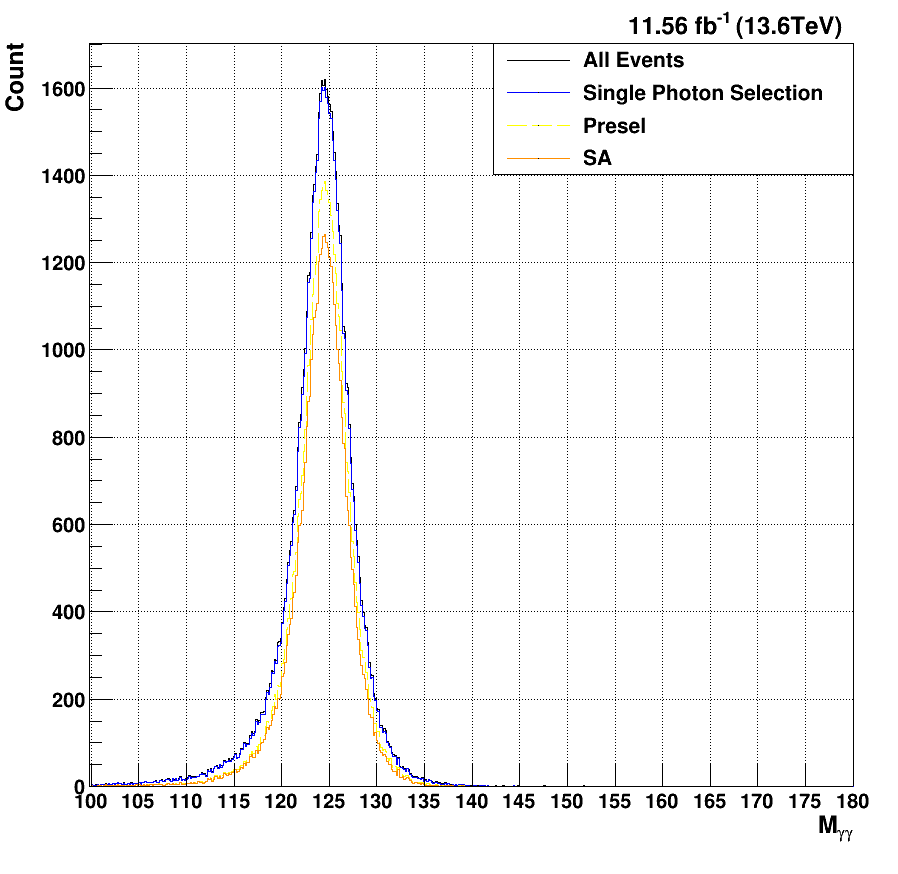
\includegraphics[width=\linewidth]{./Figures/Offline Selection Plots/0710_SinglePhoOfflineCuts_SingleSquarePlots/hggMass_All_Sig.png}
		\caption{Signal MC $M_{\gamma \gamma}$}
		\label{SinglePhoCuts:MggSig}
	\end{subfigure}\hfill
	\begin{subfigure}{0.50\linewidth}
		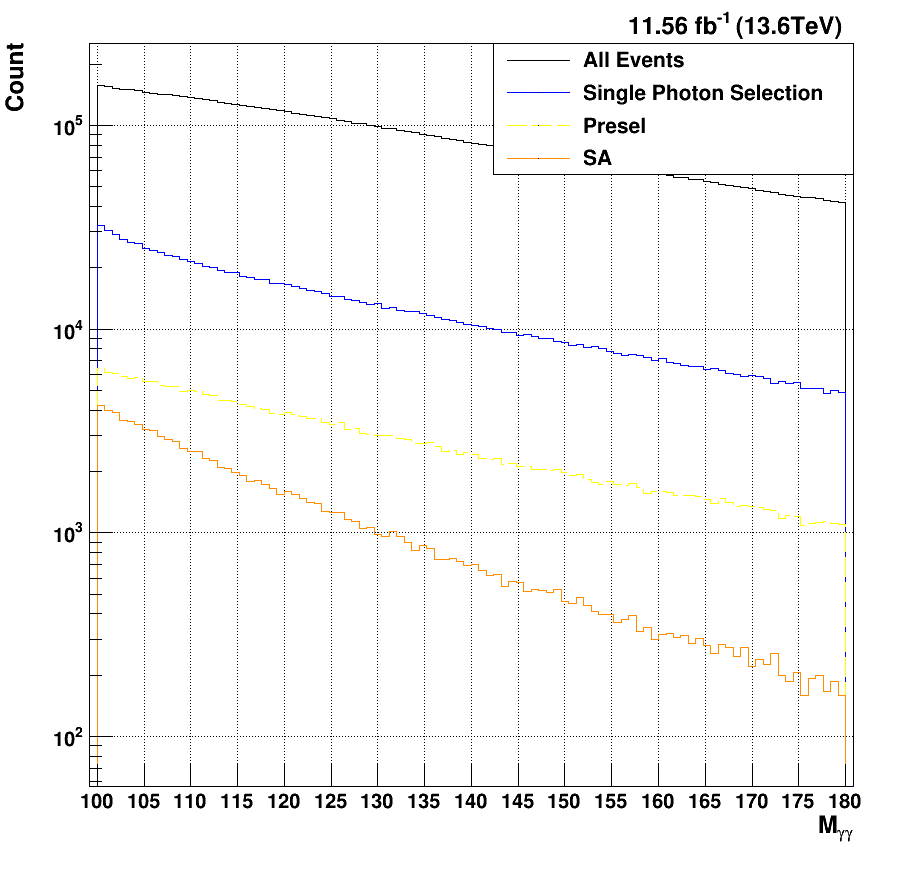
\includegraphics[width=\linewidth]{./Figures/Offline Selection Plots/0710_SinglePhoOfflineCuts_SingleSquarePlots/hggMass_All_Bkg.png}
		\caption{Data $M_{\gamma \gamma}$}
		\label{SinglePhoCuts:MggBkg}
	\end{subfigure}
	\caption{Acceptance of the MVA-HLT (blue) vs. the current standard diphoton HLT (green) for $M_{\gamma \gamma}$}
	\label{fig:SinglePhoCutsMgg}
\end{figure}

Clearly, as seen in figure \ref{fig:SinglePhoCutsMgg}, these chosen single photon cuts (in blue) leave the signal MC relatively untouched. The final chosen signal efficiency for this gluon fusion $H \rightarrow \gamma \gamma$ is 98.3\%, which is much higher than the standard single photon preselection efficiency of 78.5\%. Of course, it can be seen that the background rate is much higher -- while the standard preselection cuts achieve a background rejection of 96.8\%, the loose single photon BDT cuts only achieve an 85.9\% rejection. 

\begin{figure}[H]
	\begin{subfigure}{0.50\linewidth}
		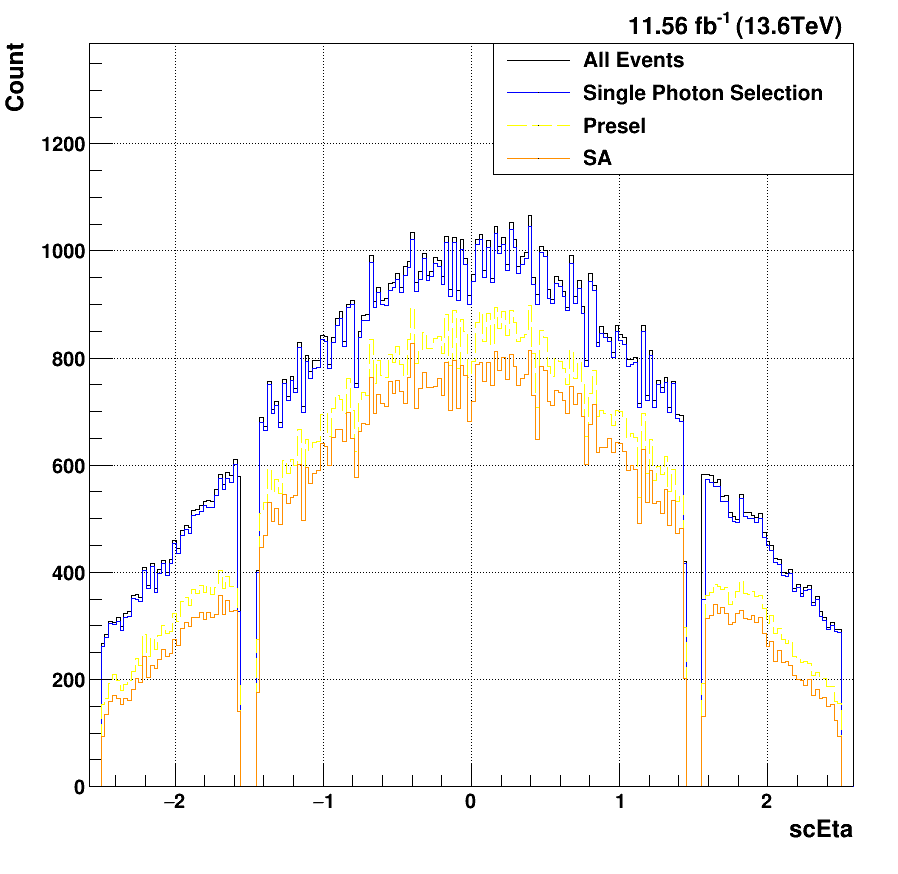
\includegraphics[width=\linewidth]{./Figures/Offline Selection Plots/0710_SinglePhoOfflineCuts_SingleSquarePlots/scEta_All_Sig.png}
		\caption{Signal MC $\eta_{SC}$}
		\label{SinglePhoCuts:EtaSig}
	\end{subfigure}\hfill
	\begin{subfigure}{0.50\linewidth}
		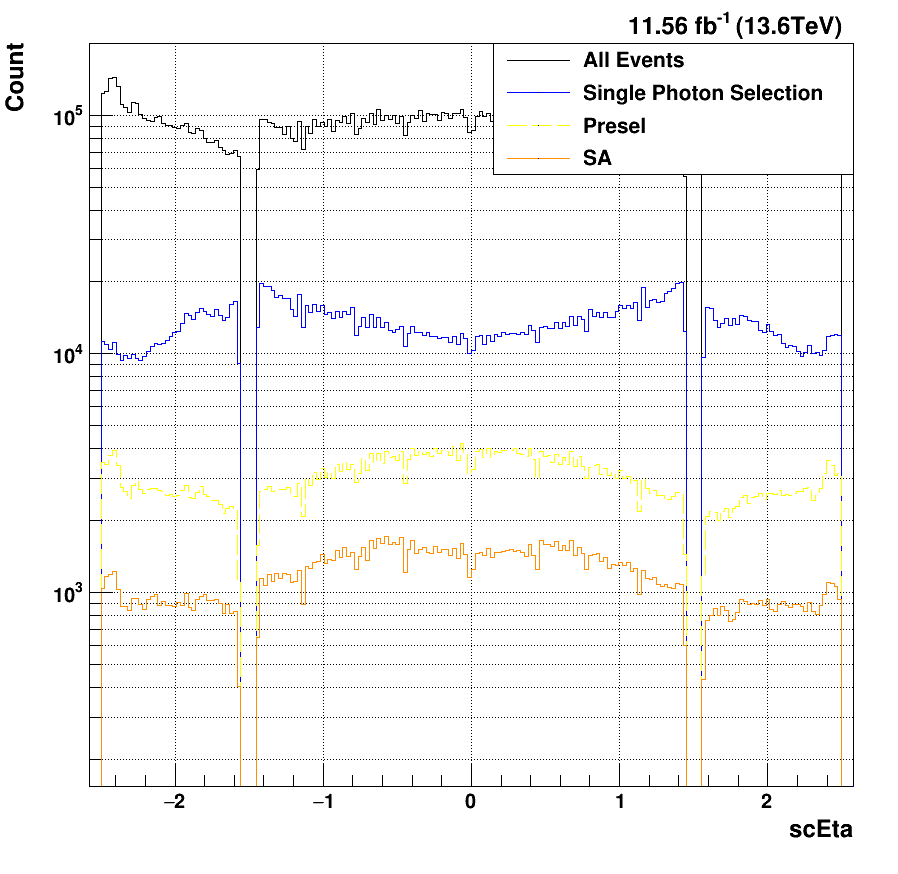
\includegraphics[width=\linewidth]{./Figures/Offline Selection Plots/0710_SinglePhoOfflineCuts_SingleSquarePlots/scEta_All_Bkg.png}
		\caption{Data $\eta_{SC}$}
		\label{SinglePhoCuts:EtaBkg}
	\end{subfigure}
	\caption{Acceptance of the MVA-HLT (blue) vs. the current standard diphoton HLT (green) for $\eta_{SC}$. Both the lead and sublead photons are plotted together.}
	\label{fig:SinglePhoCutsEta}
\end{figure}

Maximizing the kinematic acceptance of the signal events in $\eta_{SC}$ is a key consideration to any photon selection. In figure \ref{fig:SinglePhoCutsEta}, the acceptance of the different single photon selections is shown. Given that the signal acceptance is so high for these loose single photon cuts, it can be seen immediately that there are no regions of the detector shown for which the acceptance is problematic. Considering the preselection (yellow), however, a relative drop in efficiency can be seen in the low-$\eta$ regions at the start of the endcap (near $\lvert \eta \rvert$  = 1.5). Investigations showed that the hard $R_9$ cuts placed on the photons by the standard preselection are responsible for this relative dip in efficiency. Utilizing the $R_9$ in the BDT, as opposed to these hard cuts, ensures that the kinematic coverage for the loose single photon BDT selection is better than that of the standard preselection.

\begin{figure}[H]
	\begin{subfigure}{0.50\linewidth}
		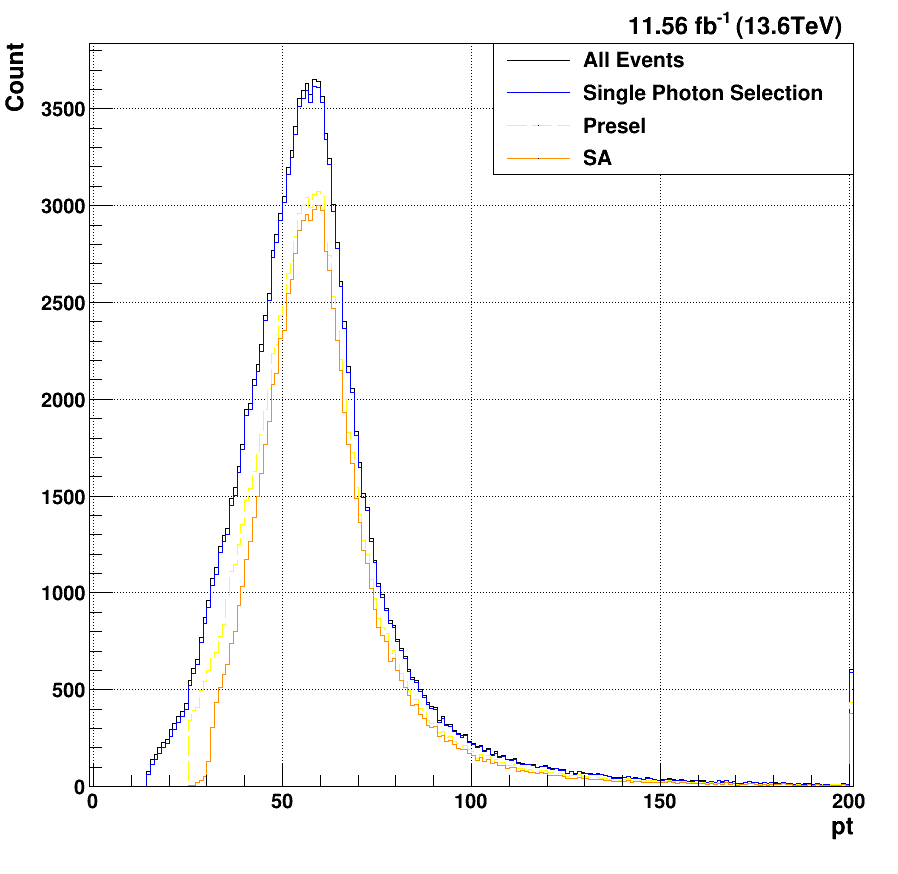
\includegraphics[width=\linewidth]{./Figures/Offline Selection Plots/0710_SinglePhoOfflineCuts_SingleSquarePlots/pt_All_Sig.png}
		\caption{Signal MC $p_{T}$}
		\label{SinglePhoCuts:PtSig}
	\end{subfigure}\hfill
	\begin{subfigure}{0.50\linewidth}
		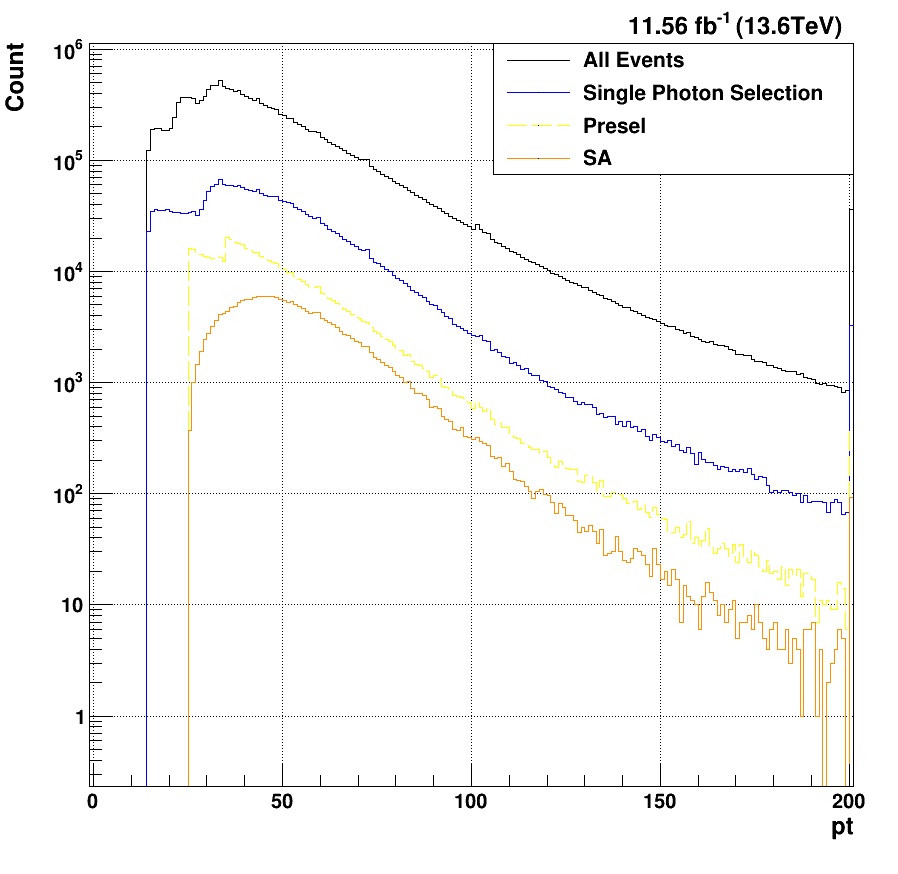
\includegraphics[width=\linewidth]{./Figures/Offline Selection Plots/0710_SinglePhoOfflineCuts_SingleSquarePlots/pt_All_Bkg.png}
		\caption{Data $p_{T}$}
		\label{SinglePhoCuts:PtBkg}
	\end{subfigure}
	\caption{Acceptance of the MVA-HLT (blue) vs. the current standard diphoton HLT (green) for $p_{T}$. Both the lead and sublead photons are plotted together.}
	\label{fig:SinglePhoCutsPt}
\end{figure}

A major advantage to these loose single photon cuts can be seen in figure \ref{fig:SinglePhoCutsPt}. Clearly, the standard preselection cuts considerably reduce the signal MC kinematic phase space by making relatively tight cuts of $p^{Lead}_{T} > 35 GeV/c^2$ and $p^{Sub}_{T} > 25 GeV/c^2$. While this also leads to a considerable reduction in data rate, the loss of good Higgs events with low-$p_T$ photons may impact future analyses with different kinematics. By comparison, the loose single photon cuts, being based entirely on the single photon BDT scores, do not noticably impact the $p_T$ distributions of either the signal or background.

\subsection{Creation of Diphoton BDT for $H \rightarrow \gamma \gamma$}\label{sec:DiphotonBDT}
With the single photon preselection cuts determined, an additional selection must be placed on the diphoton objects. The most obvious continuation of the current strategy is to create an additional MVA that now works on diphoton quantities. Previous analysis strategies have, in fact, employed a diphoton MVA for the classification of events \cite{Run2Hgg2018}. A new diphoton BDT can be constructed in reference to this, with the aim of making final cuts on this score such that the background rate is controlled while maintaining maximum signal efficiency.

While the goal of the single photon BDTs is to reject individual candidates that appear to not be photons, the diphoton BDT aims to properly differentiate diphton candidates coming from $H \rightarrow \gamma \gamma$ from both events that do not contain two real photons and events with two real photons originating from background processes. As a result, the inputs to this model will consist primarily of lead and sublead single photon variables. By providing both the lead and sublead values to one model, correlations can be found that ensure that selected events contain two real photons with the necessary kinematics to possibly comprise a signal event. Below, in table \ref{tab:DiphotonBDTInputs}, each of the input variables is listed and described. These were largely adopted from the Run2 Diphoton photonID, with a few differences. 
\begin{table}
	\centering
	\caption{Table of diphoton BDT input variable names, and a short description of each.}
	\label{tab:DiphotonBDTInputs}
	\begin{tabular}{ | c | c | } 
		\hline
		\textbf{Variable Name} & \textbf{Description} \\
		\Xhline{2pt}
	  	$p^{Lead}_{T}/M_{\gamma \gamma}$ and $p^{Sub}_{T}/M_{\gamma \gamma}$ & The mass-normalized $p_T$ for each photon \\ 
		\hline
		$\eta^{Lead}_{sc}$ and $\eta^{Sub}_{sc}$ & The supercluster $\eta$ for each photon  \\ 
		\hline
		$BDT^{Lead}_{\gamma + jet}$ and $BDT^{Sub}_{\gamma + jet}$& The $\gamma + jet$ BDT score for each photon\\ 
		\hline
		$BDT^{Lead}_{Data/MC}$ and $BDT^{Sub}_{Data/MC}$& The Data/MC BDT score for each photon\\ 
		\hline
		Lead and Sublead Electron Veto &  A boolean to reject photons origininating from electrons\\ 
		\hline
		$cos(\Delta \phi)$ &  The cosine of the $\phi$ separation of the two photons \\ 
		\hline
		$\sigma(M_{\gamma \gamma})/M_{\gamma \gamma}$ & A relative mass resolution estimate \\ 
		\hline
	\end{tabular}
\end{table}

Since the goal of this model is to differentiate signal diphoton combinations from those in the background, signal MC and data can again be used for the signal and background for the BDT, as with the data/MC BDT described above. Again, the input variable distributions can be examined to see the separation between signal and background class events.

The first two variables are related directly to the kinematics of the diphoton object, and therefore are not split into lead and sublead values. The first, $\sigma(M_{\gamma \gamma})/M_{\gamma \gamma}$, provides a relative invariant mass resolution estimate of the diphoton combination. It can clearly be seen in figure \ref{DiphoVars:sigmaMovrM}, that there is great separation between the signal MC and data events. The signal MC tends to have a much lower $\sigma(M_{\gamma \gamma})/M_{\gamma \gamma}$, which corresponds to a higher mass resolution. This is to be expected, as the two selected photons in the $H \rightarrow \gamma \gamma$ are much more likely to come from a resonant process than those in the  data. The cos($\Delta \phi$), however, does not exhibit the same strong separation. This variable aims to measure the separation in $\phi$ of the two selected photon candidates. Based on the other selections at play, however, it seems that this variable will not be a strong discrimination variable.

\begin{figure}[H]
	\begin{subfigure}{0.50\linewidth}
		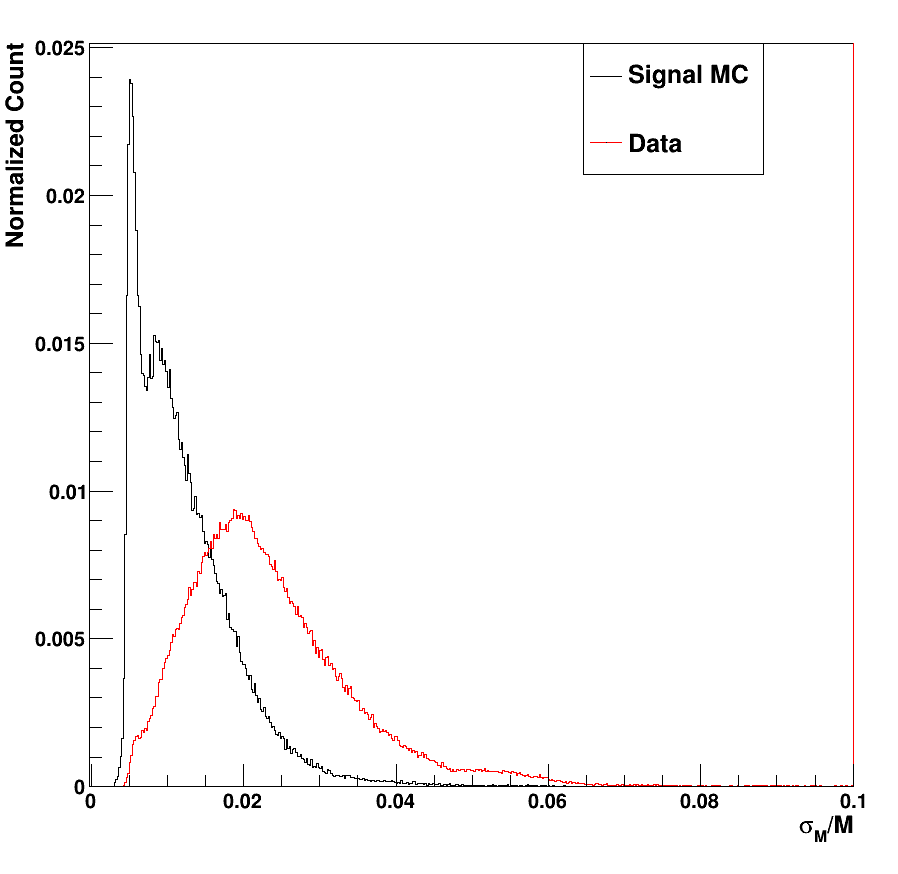
\includegraphics[width=\linewidth]{./Figures/Offline Selection Plots/0709_Updated_DiphotonBDT_TrainingPlots/sigMovrM.png}
		\caption{$\sigma(M_{\gamma \gamma})/M_{\gamma \gamma}$}
		\label{DiphoVars:sigmaMovrM}
	\end{subfigure}\hfill
	\begin{subfigure}{0.50\linewidth}
		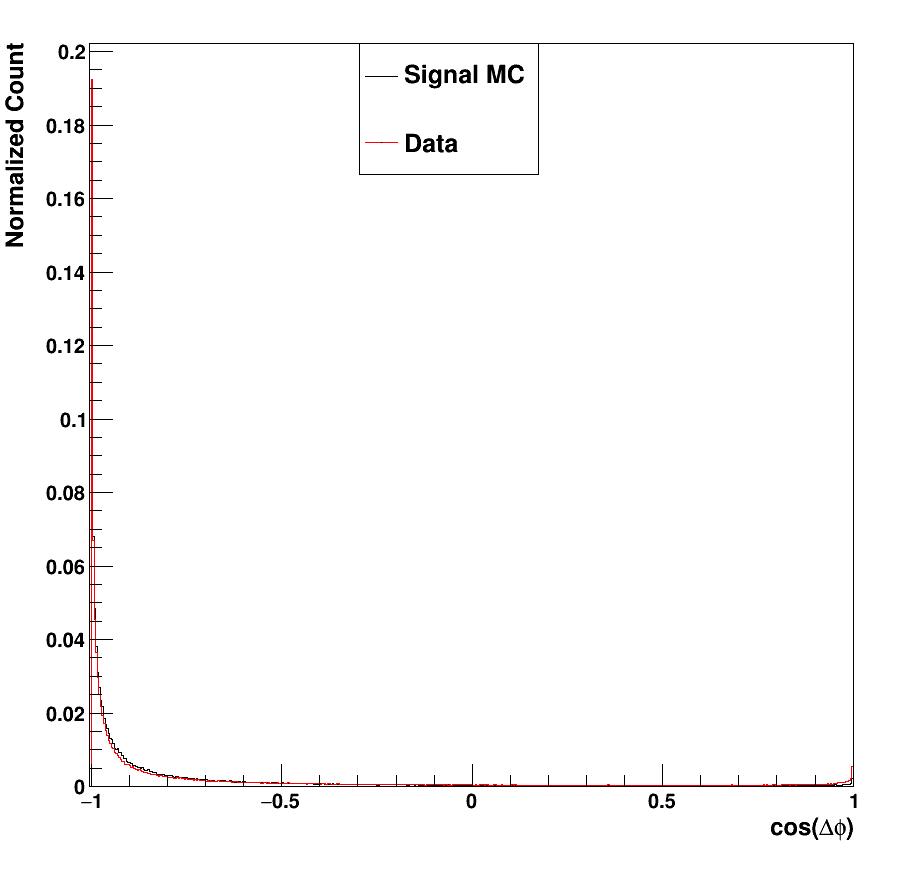
\includegraphics[width=\linewidth]{./Figures/Offline Selection Plots/0709_Updated_DiphotonBDT_TrainingPlots/cosDPhi.png}
		\caption{cos($\Delta \phi$)}
		\label{DiphoVars:cosDPhi}
	\end{subfigure}
	\caption{The two per-event diphoton input variables,$\sigma(M_{\gamma \gamma})/M_{\gamma \gamma}$ and cos($\Delta \phi$). The signal MC is in black, whereas the data events are in red.}
	\label{fig:DiphoVars1}
\end{figure}

The next two pairs of input variables are the single photon BDT scores. Firstly, the $\gamma$ + Jet single photon BDT scores are shown below in figure \ref{fig:DiphoVars2}. As with all XGBoost BDT binary classification scores, a value near 0 shows that the algorithm has identified the photon as being part of the background class, while a score near 1 corresponds to an event identified as part of the signal class. For the signal MC, it can be seen that the scores peak very well near 1. This is to be expected, as the signal MC photons here are matched to a generated photon and therefore guaranteed to be a real photon. This effect is clear for both the lead and sublead photons.

Clearly, however, the background photons in red are not constrained entirely near 0. In fact, there are two peaks in both the lead and sublead score distributions. While many of the background photon candidates can easily be assigned a score near 0, there are also a large number for which the $\gamma$ + Jet scores are not adequate to differentiate the background from the signal. This likely due, at least in part, to the composition of the data overall. While many of the data events consist of dijet QCD background, there are likely many events for which one or even two real photons have been selected. This is exacerbated by the triggers required for this training sample; here, since either the MVA-HLT trigger or the standard diphoton trigger must be passed to enter the training sample, the odds of a data event containing one or two real photons is much higher than it would be for other data samples. This demonstrate why the $\gamma$ + Jet BDT alone is not adequate to correctly differentiate between signal and background events.  
\begin{figure}[H]
	\begin{subfigure}{0.50\linewidth}
		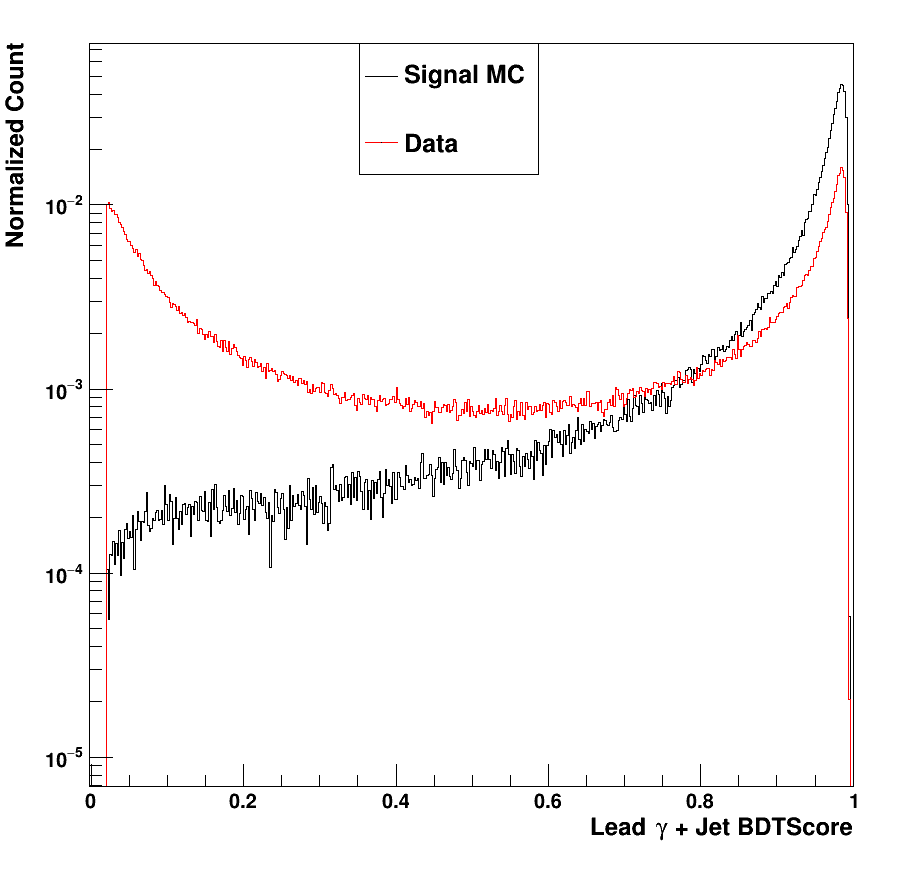
\includegraphics[width=\linewidth]{./Figures/Offline Selection Plots/0709_Updated_DiphotonBDT_TrainingPlots/leadGJetXGBScore.png}
		\caption{Lead $\gamma$ + Jet BDT Score}
		\label{DiphoVars:leadGJetXGBScore}
	\end{subfigure}\hfill
	\begin{subfigure}{0.50\linewidth}
		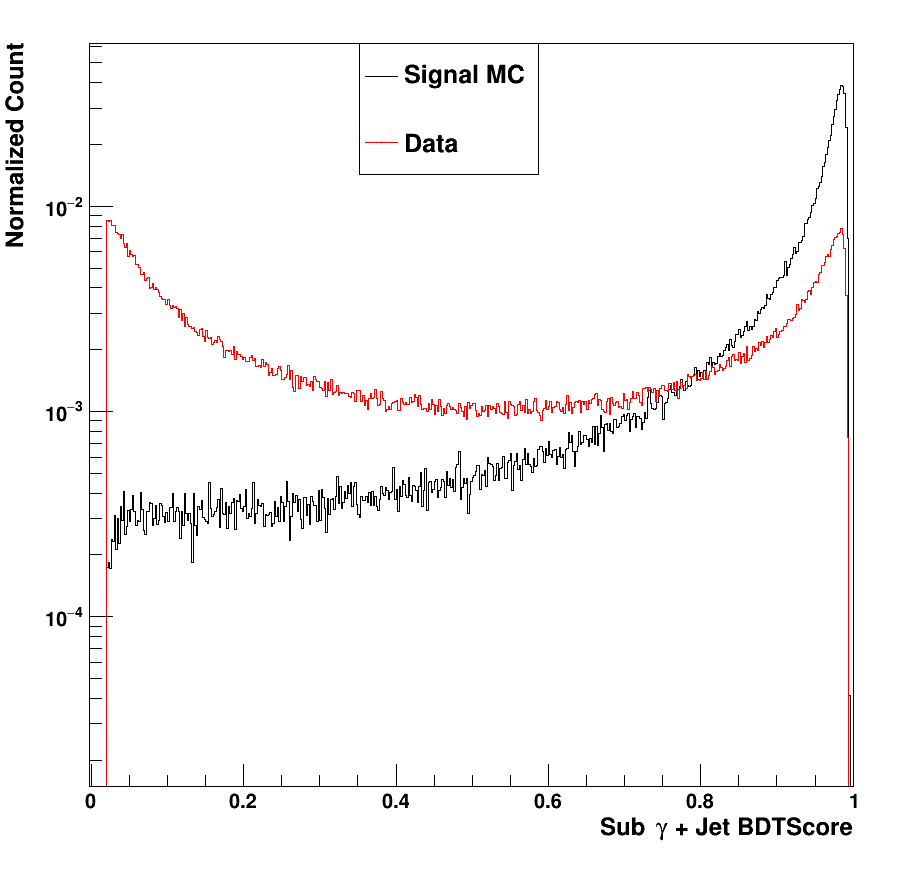
\includegraphics[width=\linewidth]{./Figures/Offline Selection Plots/0709_Updated_DiphotonBDT_TrainingPlots/subGJetXGBScore.png}
		\caption{Sub $\gamma$ + Jet BDT Score}
		\label{DiphoVars:subGJetXGBScore}
	\end{subfigure}
	\caption{The lead and sublead $\gamma$ + Jet XGBoost BDT scores. The signal MC is in black, whereas the data events are in red.}
	\label{fig:DiphoVars2}
\end{figure}

Secondly, the data/MC scores for both the lead and sublead photons are shown in figure \ref{fig:DiphoVars3} on a logarithmic scale. As expected, there is clear separation between the signal MC in black and the data in red. It is expected that the signal MC distributions will largely cluster near 1, which corresponds to a positive identification as signal. While this is true for both the lead and sublead scores, the identification of the background is perhaps a stronger effect. It can be seen that the data events are very closely clustered near 0. Very few of the background events, on the other hand, are placed near a score of 1. 

Similarly to the $\gamma$ + Jet single photon BDT, then, it is clear that this data/MC BDT is not adequate alone to differentiate signal and background. The diphoton BDT, then, is a crucial step of the signal and background selection; by having access to both the single photon BDTs, the diphoton BDT can construct correlations that allow the final model to be considerably more discerning than input scores it uses. As will be shown in chapter \ref{chapter:Results}, this works to great effect. 

\begin{figure}
	\begin{subfigure}{0.50\linewidth}
		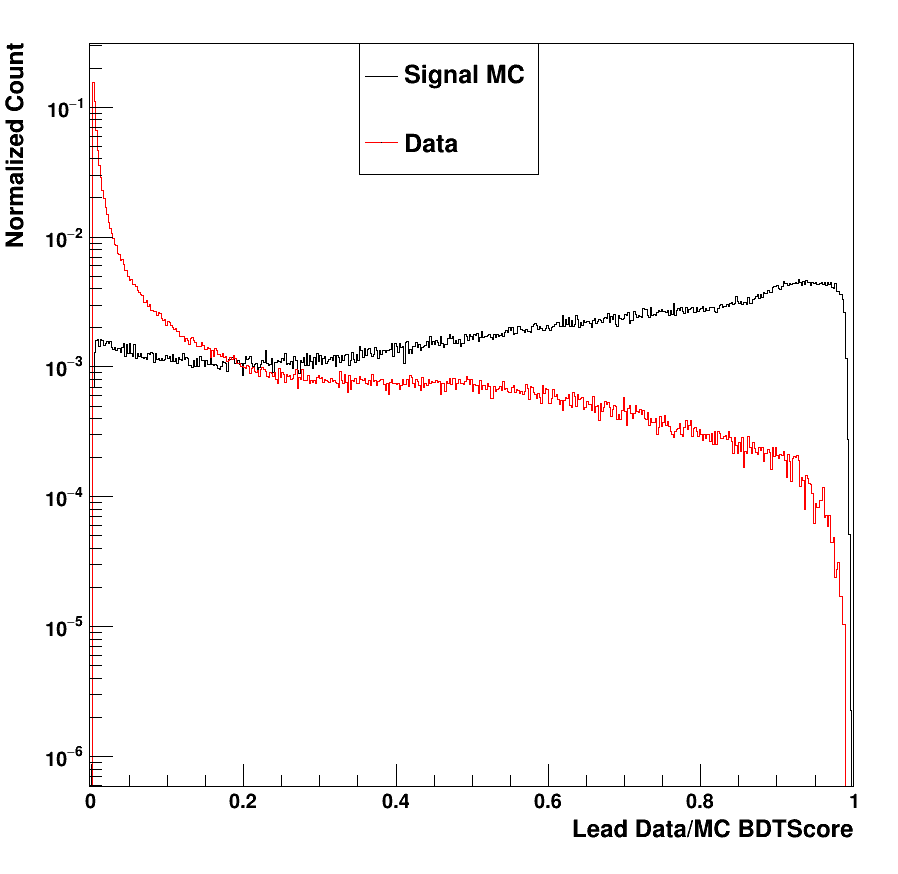
\includegraphics[width=\linewidth]{./Figures/Offline Selection Plots/0709_Updated_DiphotonBDT_TrainingPlots/leadDataMCXGBScore.png}
		\caption{Lead Data/MC BDT Score}
		\label{DiphoVars:leadDataMCXGBScore}
	\end{subfigure}\hfill
	\begin{subfigure}{0.50\linewidth}
		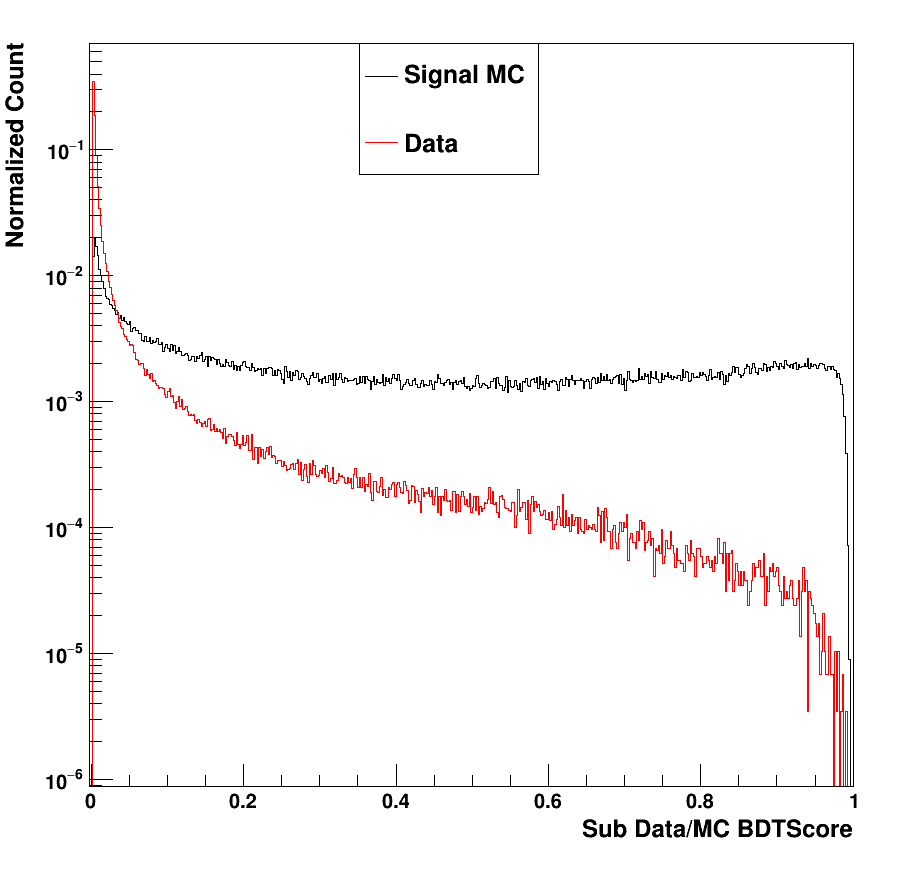
\includegraphics[width=\linewidth]{./Figures/Offline Selection Plots/0709_Updated_DiphotonBDT_TrainingPlots/subDataMCXGBScore.png}
		\caption{Sub Data/MC BDT Score}
		\label{DiphoVars:subDataMCXGBScore}
	\end{subfigure}
	\caption{The lead and sublead Data/MC XGBoost BDT scores. The signal MC is in black, whereas the data events are in red.}
	\label{fig:DiphoVars3}
\end{figure}

While the single photon quality scores given by the single photon BDTs are quite helpful, the diphoton kinematics are additionally a very strong source of discrimination power. As sean for both the lead (figure \ref{DiphoVars:leadEta}) and sublead (figure \ref{DiphoVars:leadEta}) $\eta_{SC}$ distributions, the shape of the single Higgs signal MC in black and the data in red are quite different. Due to the kinematics of the Higgs production, as discussed in \ref{chapter:Theory}, the signal MC tends to be much more central in the barrel detector (closer to perpendicular to the beamline). Meanwhile, in the endcaps, the amount of signal photons rapidly drops as the edges of the chose $\eta_{SC}$ range are approached. Due to this good separation between signal and background, the $\eta_{SC}$ of the lead and sublead photon provide good discrimination power to the binary classifier BDT.
\begin{figure}[H]
	\begin{subfigure}{0.50\linewidth}
		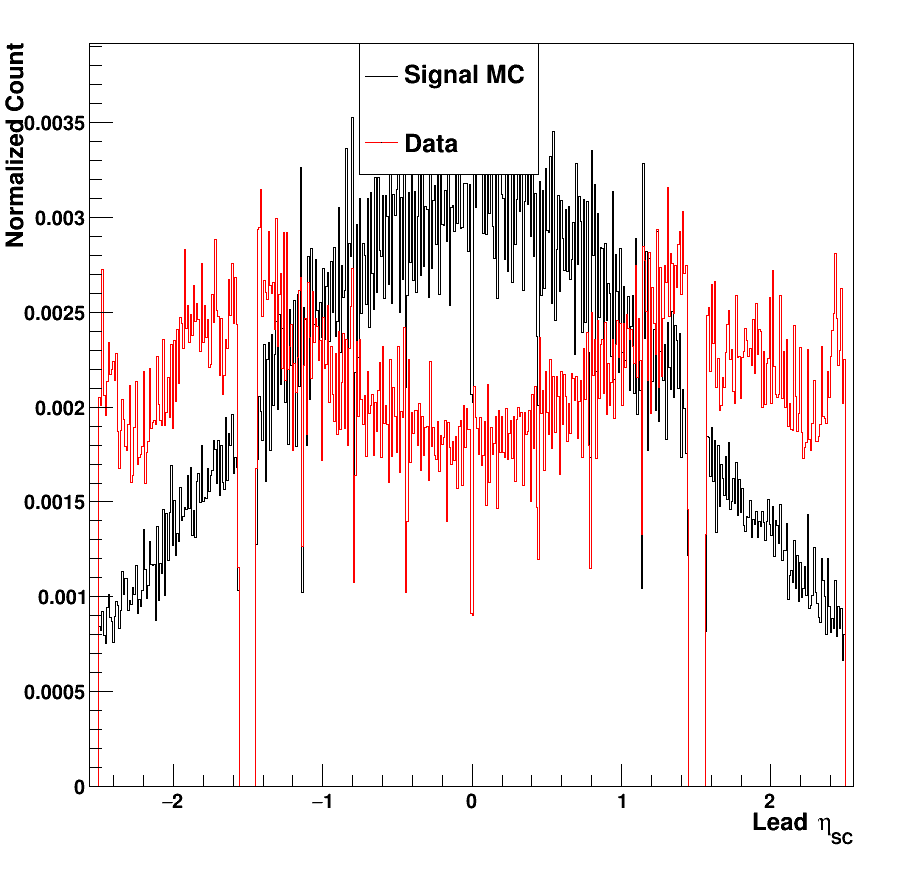
\includegraphics[width=\linewidth]{./Figures/Offline Selection Plots/0709_Updated_DiphotonBDT_TrainingPlots/leadScEta.png}
		\caption{Lead $\eta_{SC}$}
		\label{DiphoVars:leadEta}
	\end{subfigure}\hfill
	\begin{subfigure}{0.50\linewidth}
		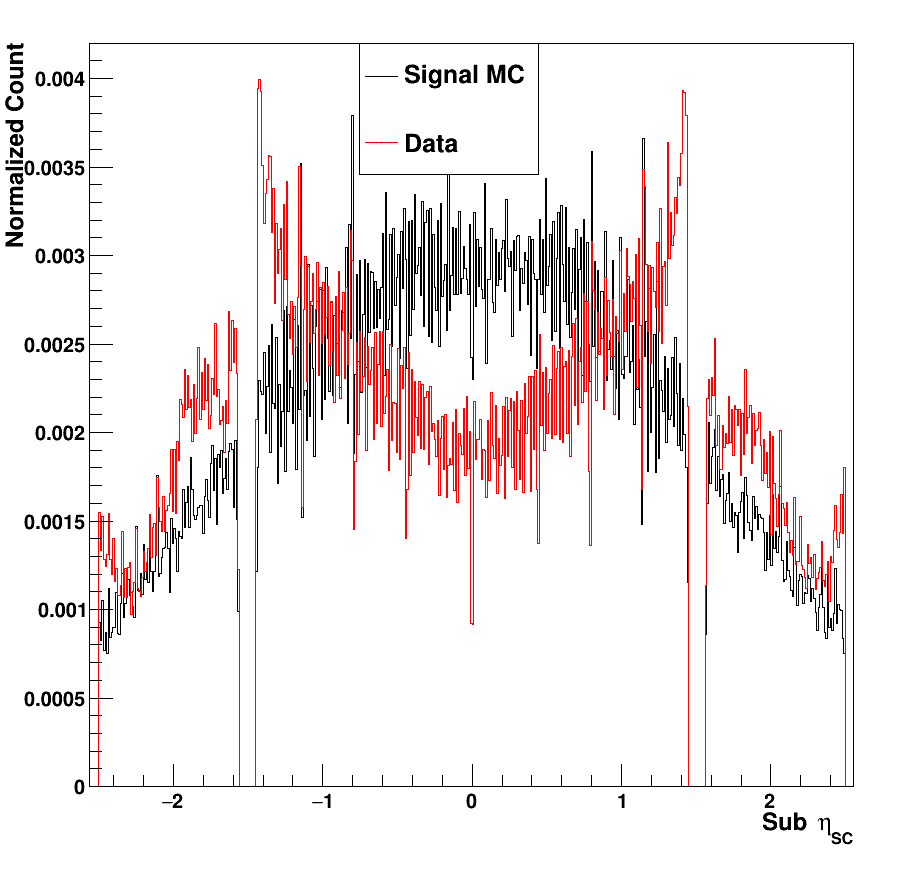
\includegraphics[width=\linewidth]{./Figures/Offline Selection Plots/0709_Updated_DiphotonBDT_TrainingPlots/subScEta.png}
		\caption{Sub $\eta_{SC}$}
		\label{DiphoVars:subEta}
	\end{subfigure}
	\caption{The lead and sublead $\eta_{SC}$. The signal MC is in black, whereas the data events are in red.}
	\label{fig:DiphoVars4}
\end{figure}

The other diphoton kinematic quantities used by the diphoton BDT are the $p_T/M_{\gamma \gamma}$ of the two selected photons. This mass-normalized measure of the photon candidates' transverse momentum is used in the standard diphoton preselection given its great discrimination power. Of course, if hard cuts on a variable are successful in separating signal from background, a BDT should be able to leverage the information to even greater effect. Furthermore, as with the $p_T$ cuts, removing the hard cuts on this variable considerably improve the kinematic coverage of the offline selection. In figure \ref{fig:DiphoVars5}, a clear separation between the signal and background events can be seen for both the lead and sublead photon candidates. Paired with the corresponding $\eta_{SC}$ values, this lends considerable kinematic discrimination power to the diphoton BDT.

\begin{figure}[H]
	\begin{subfigure}{0.50\linewidth}
		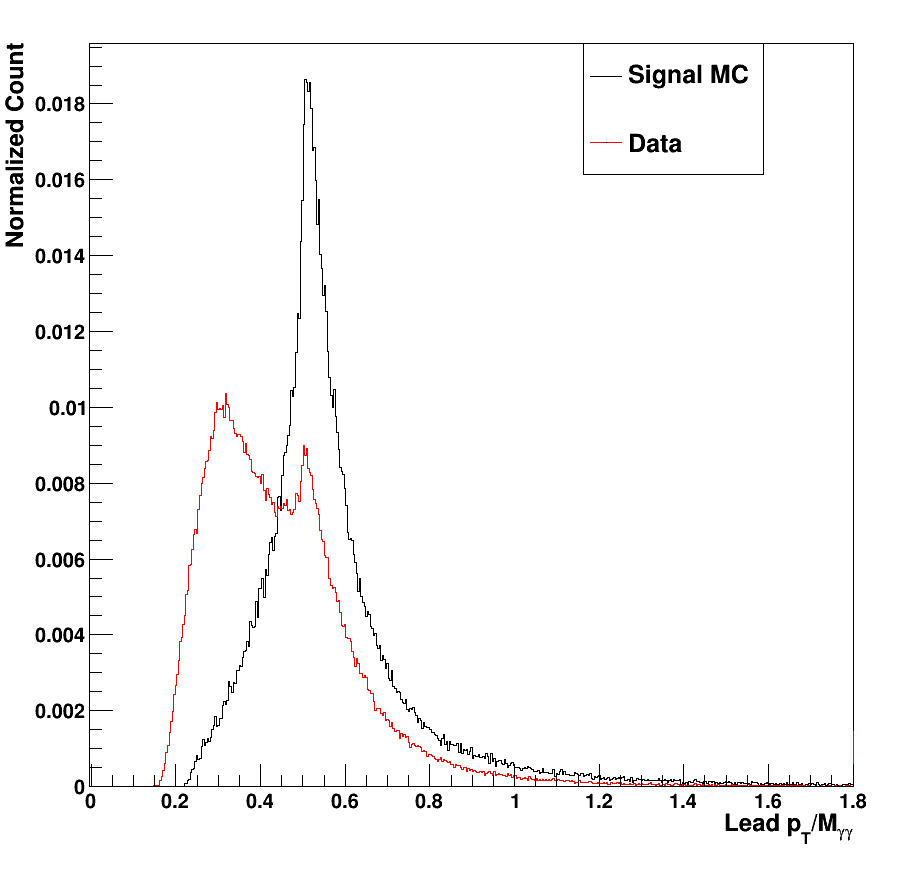
\includegraphics[width=\linewidth]{./Figures/Offline Selection Plots/0709_Updated_DiphotonBDT_TrainingPlots/leadPtOvrM.png}
		\caption{Lead $p_{T}/M_{\gamma \gamma}$}
		\label{DiphoVars:leadPtM}
	\end{subfigure}\hfill
	\begin{subfigure}{0.50\linewidth}
		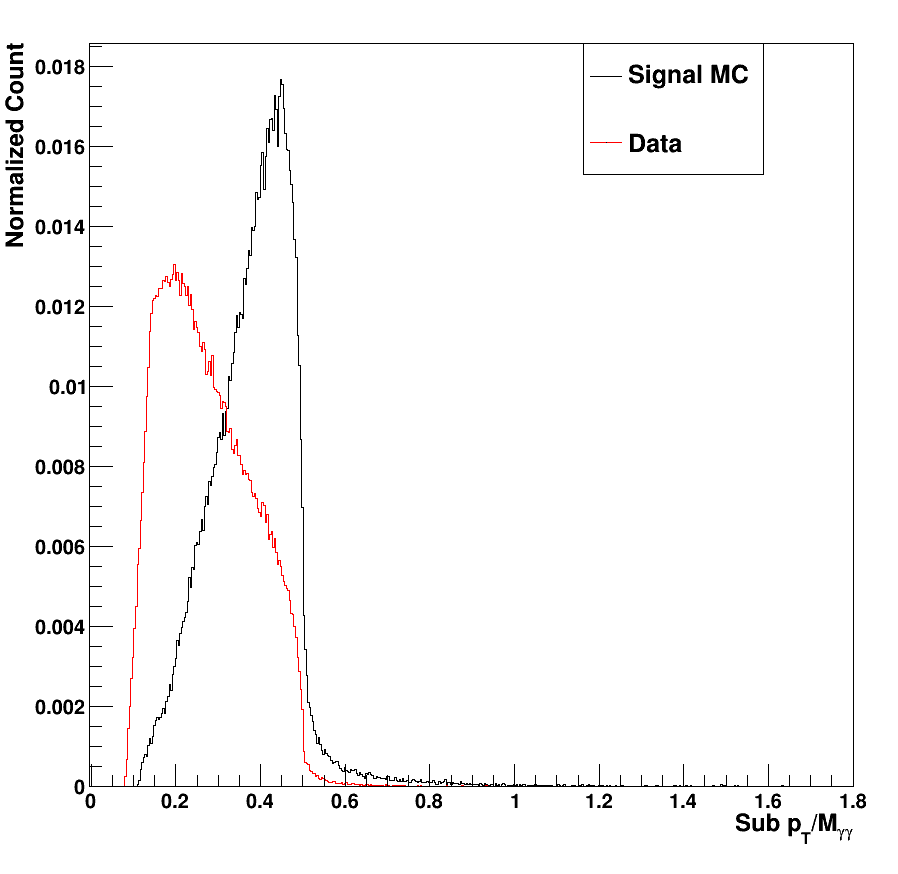
\includegraphics[width=\linewidth]{./Figures/Offline Selection Plots/0709_Updated_DiphotonBDT_TrainingPlots/subPtOvrM.png}
		\caption{Sub $p_{T}/M_{\gamma \gamma}$}
		\label{DiphoVars:subPtM}
	\end{subfigure}
	\caption{The lead and sublead $p_{T}/M_{\gamma \gamma}$. The signal MC is in black, whereas the data events are in red.}
	\label{fig:DiphoVars5}
\end{figure}

Finally, the electron veto values can be used to help differentiate between photons and electrons in the final selection. As discussed in section \ref{sec:OfflineReco}, photons and electrons are quite hard to differentiate purely from ECal information. The electron veto was designed to leverage charged track information to provide a conversion-safe way to reject electrons from photon candidates \cite{OfflineReco2021}. This quantity has not historically been deployed in the diphotonMVA; since the standard preselection generally makes a hard requirement on the electron veto, there is no need to use it in the diphotonMVA. By adding the lead and sublead electron veto decision to the diphoton BDT, however, the information can be correlated with the other variables provided to more elegantly reject electrons in the data while still maximizing the signal efficiency.

The values of the electron veto are shown in figure \ref{fig:DiphoVars6}. Since this is just a veto decision, the variable is saved as a boolean. As a result, the plots show a value of 0 for false (failing the electron veto) and 1 for true (passing the electron veto). A very clear separation can be seen between the signal MC (black) and data (red). Very few of the selected signal MC lead or sublead photon candidates fail the electron veto, wheareas there are a considerable portion of the data events that fail. It can be seen, however, that there are still many data events that pass the electron veto. 

\begin{figure}[H]
	\begin{subfigure}{0.50\linewidth}
		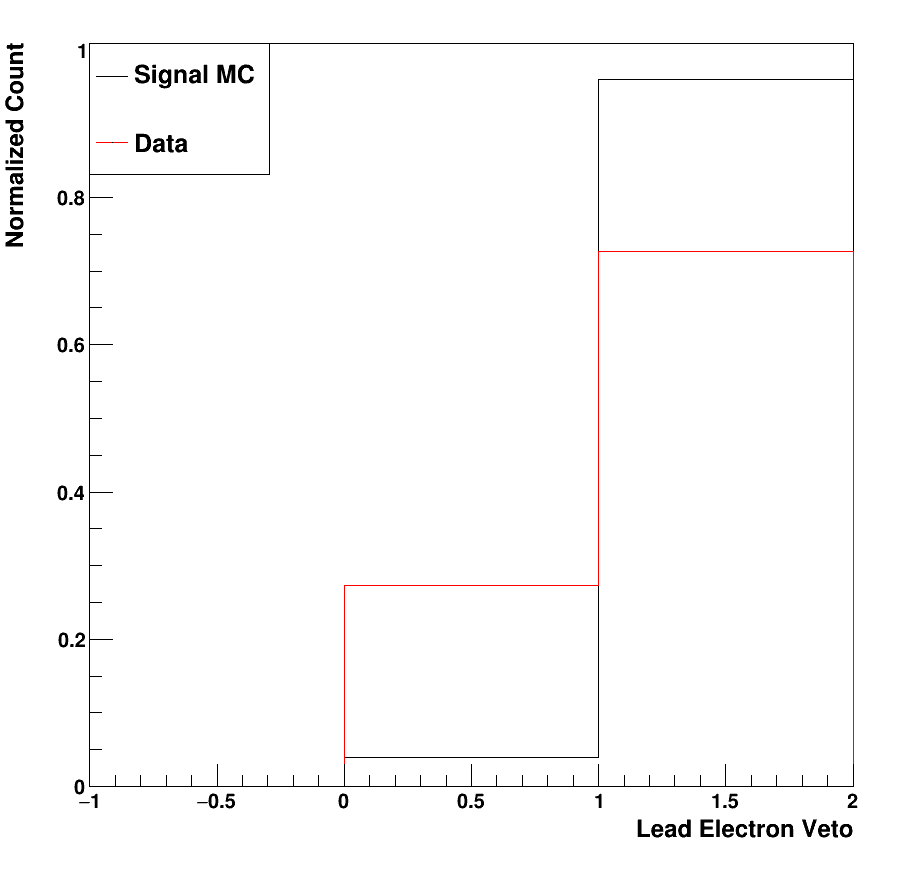
\includegraphics[width=\linewidth]{./Figures/Offline Selection Plots/0709_Updated_DiphotonBDT_TrainingPlots/leadElectronVeto.png}
		\caption{Lead Electron Veto}
		\label{DiphoVars:leadEVeto}
	\end{subfigure}\hfill
	\begin{subfigure}{0.50\linewidth}
		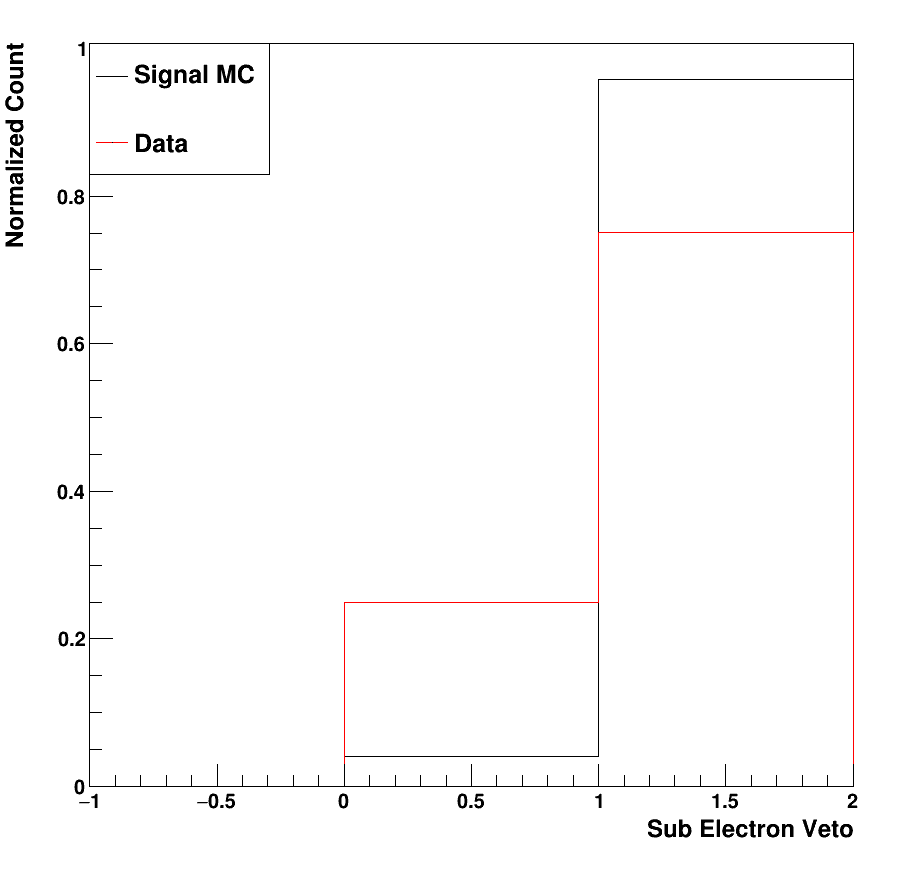
\includegraphics[width=\linewidth]{./Figures/Offline Selection Plots/0709_Updated_DiphotonBDT_TrainingPlots/subElectronVeto.png}
		\caption{Sub Electron Veto}
		\label{DiphoVars:subEVeto}
	\end{subfigure}
	\caption{The lead and sublead electron veto. The signal MC is in black, whereas the data events are in red.}
	\label{fig:DiphoVars6}
\end{figure}

As with the other two BDTs, the hyperparameters must of course be optimized once the input variables are selected. This was, again, a relatively experimental process. Given the reduced number of input variables relative to the single photon BDTs, lower maximum depths were explored. A max depth of 10 was selected in conjunction with a learning rate of 0.1. This lower max depth and higher learning rate allows to model to still leverage the reduced number of input variables without considerable overtraining.

\subsubsection{A Data/MC BDT for $HH \rightarrow b \bar{b} \gamma \gamma$}

Of course, since the Data/MC and diphoton BDTs are trained using signal MC and data, they should be retrained for samples with markedly different input features. As discussed in chapter \ref{chapter:Theory}, the kinematics of the $HH \rightarrow b \bar{b} \gamma \gamma$ differ considerably from the $H \rightarrow \gamma \gamma$. Therefore, the same process of training and evaluation must be repeated for these new samples. While the same data samples are used for this updated analysis, the $HH \rightarrow b \bar{b} \gamma \gamma$ workflow applies additional cuts to the $b \bar{b}$ object as discussed in section \ref{sec:HiggsDNA}. The same input variable distributions for the Data/MC BDT are displayed in figures \ref{fig:DiHiggs:DataMCVars1}-\ref{fig:DiHiggs:DataMCVars6} for these new samples. Major differences between the single and DiHiggs samples will be noted.

\begin{figure}[H]
	\begin{subfigure}{0.50\linewidth}
		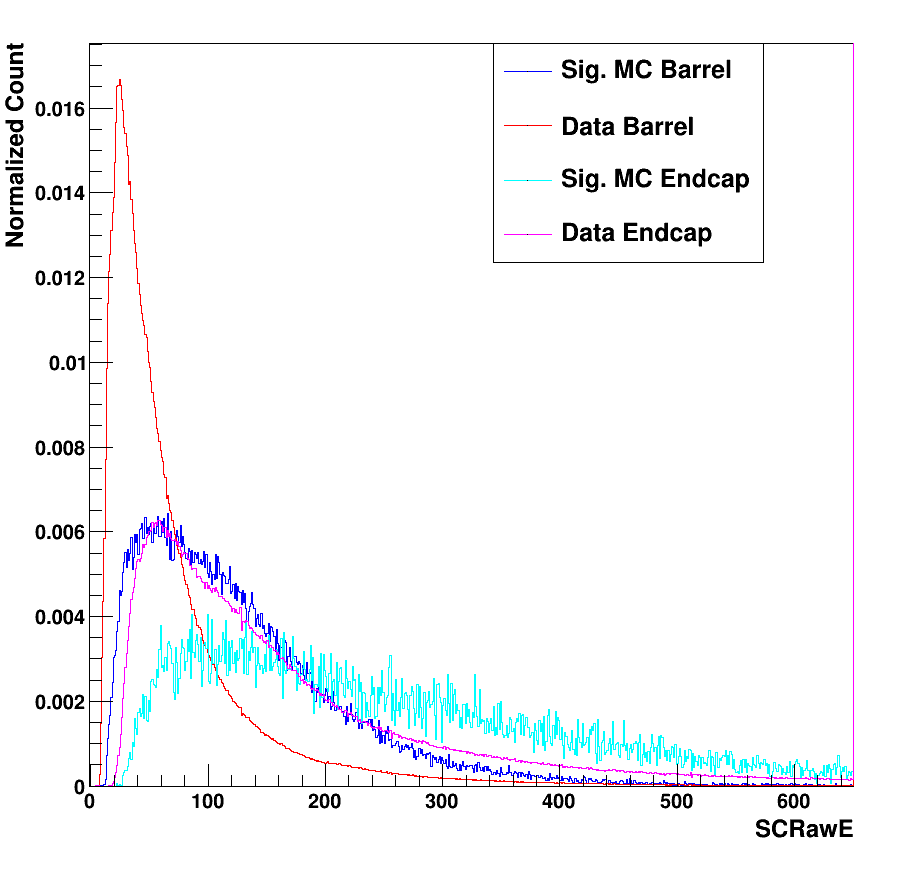
\includegraphics[width=\linewidth]{./Figures/Offline Selection Plots/DiHiggs/0715_DataMC_TrainingPlots/SCRawE.png}
		\caption{Raw Energy}
		\label{DataMCVars:DiHiggs:RawE}
	\end{subfigure}\hfill
	\begin{subfigure}{0.50\linewidth}
		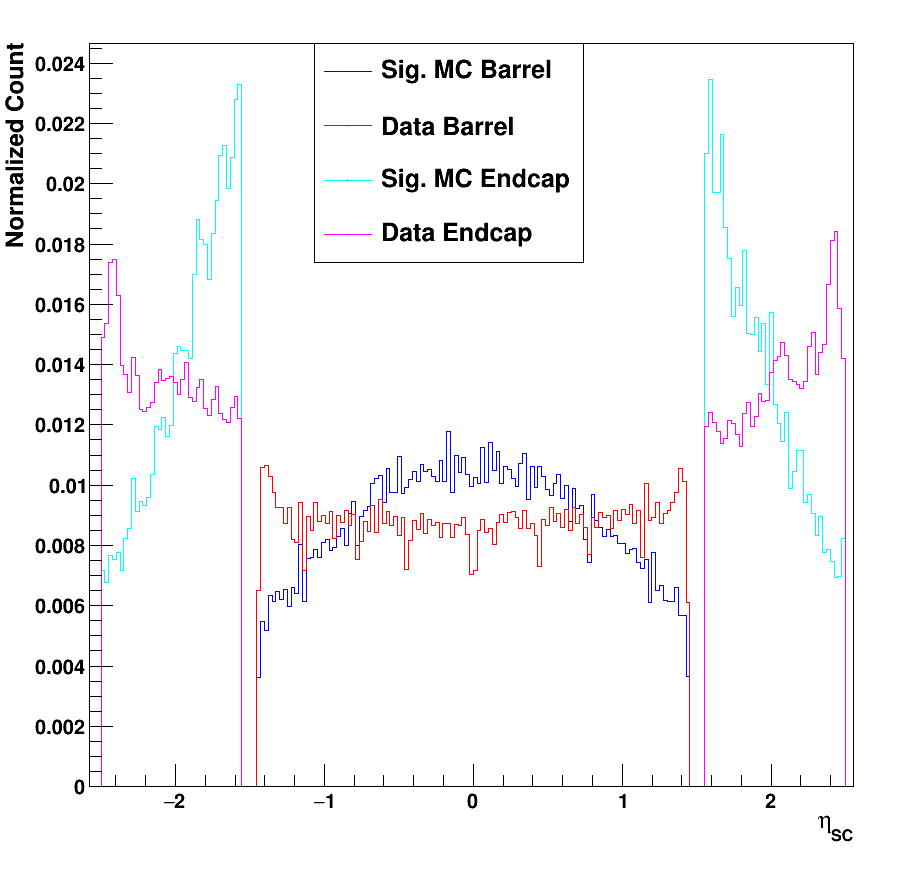
\includegraphics[width=\linewidth]{./Figures/Offline Selection Plots/DiHiggs/0715_DataMC_TrainingPlots/scEta.png}
		\caption{$\eta_{SC}$}
		\label{DataMCVars:DiHiggs:eta}
	\end{subfigure}
	\caption{Plots of the Supercluster raw energy and $\eta{SC}$. The signal MC is shown in dark blue for the barrel and light blue for the endcap, whereas the data (background) is shown in red for the barrel and pink for the endcap.}
	\label{fig:DiHiggs:DataMCVars1}
\end{figure}

A major difference in $\eta_{SC}$ exists relative to the single H, as seen in figure \ref{fig:DiHiggs:DataMCVars1}. While the signal MC is relatively similar in the barrel, the endcap is far more concentrated at lower-$\eta$ values. The data, on the other hand, is considerably more flat in both the endcap and barrel due to the changed kinematics based on the requirements placed on finding a $b \bar{b}$ pair. On the whole, this leads the $\eta_{SC}$ being used more strongly by the DiHiggs Data/MC BDT. Since less of the MC is in the extreme regions of the endcap, it will be shown that the selection is biased away from selecting data in these regions.

\begin{figure}[H]
	\begin{subfigure}{0.50\linewidth}
		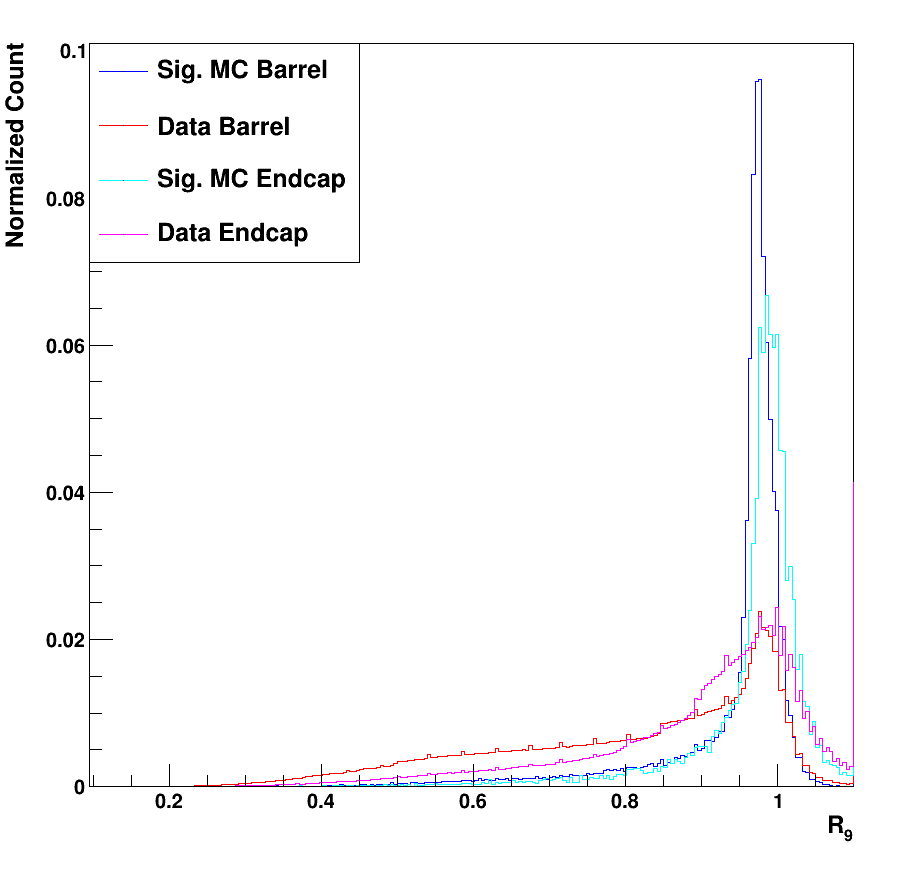
\includegraphics[width=\linewidth]{./Figures/Offline Selection Plots/DiHiggs/0715_DataMC_TrainingPlots/r9.png}
		\caption{$R_{9}$}
		\label{DataMCVars:DiHiggs:r9}
	\end{subfigure}\hfill
	\begin{subfigure}{0.50\linewidth}
		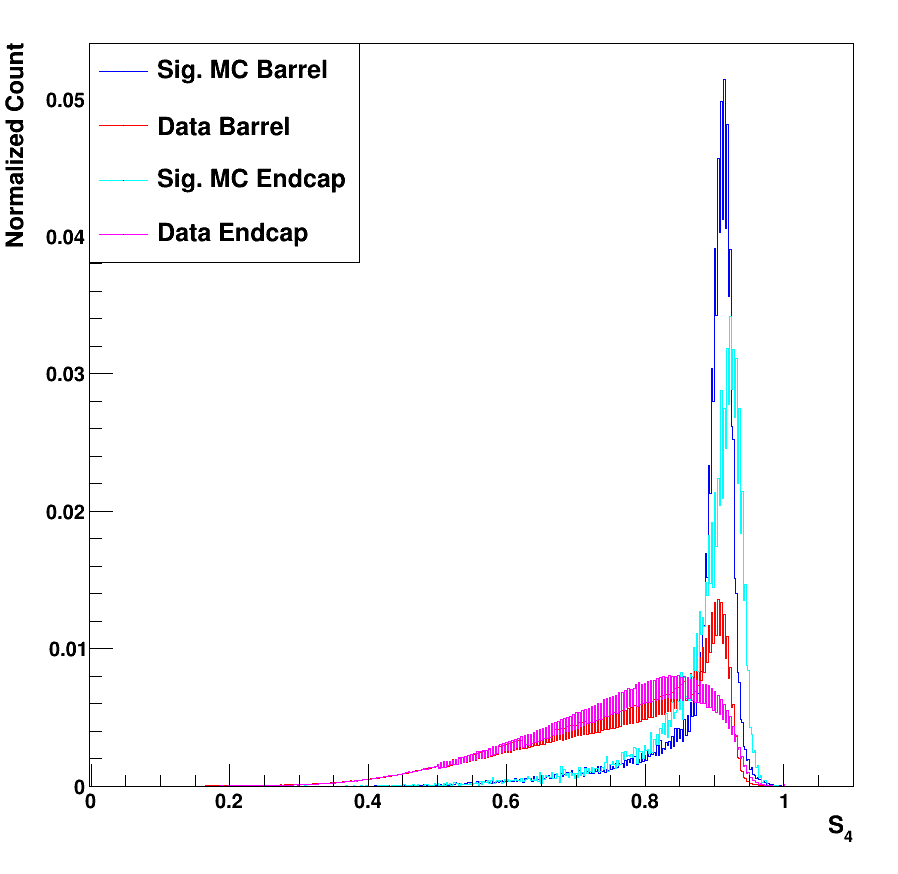
\includegraphics[width=\linewidth]{./Figures/Offline Selection Plots/DiHiggs/0715_DataMC_TrainingPlots/s4.png}
		\caption{$S_{4}$}
		\label{DataMCVars:DiHiggs:s4}
	\end{subfigure}
	\caption{Plots of the $R_9$ and $S_4$. The signal MC is shown in dark blue for the barrel and light blue for the endcap, whereas the data (background) is shown in red for the barrel and pink for the endcap.}
	\label{fig:DiHiggs:DataMCVars2}
\end{figure}

Relative to the data selected by the single Higgs workflow, the DiHiggs data selection has considerably lower values on average of both the $R_9$ and $S_4$. This leads to a clearer separation between the signal and background for both the barrel and endcap events.

\begin{figure}[H]
	\begin{subfigure}{0.50\linewidth}
		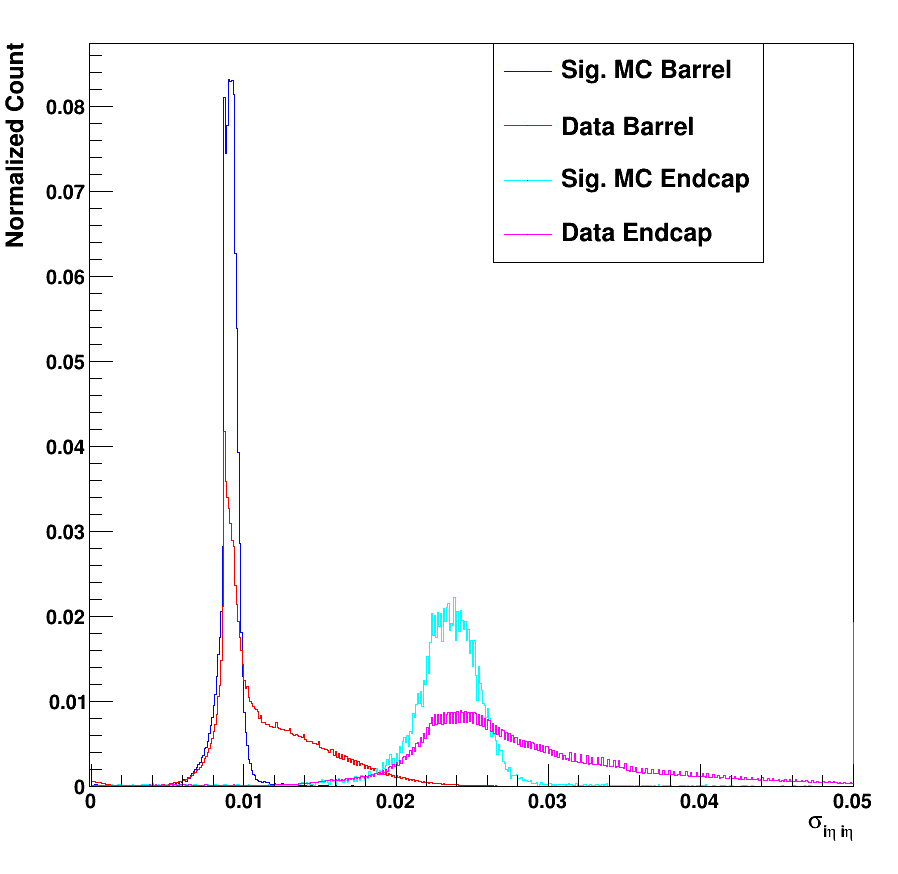
\includegraphics[width=\linewidth]{./Figures/Offline Selection Plots/DiHiggs/0715_DataMC_TrainingPlots/sigmaIetaIeta.png}
		\caption{$\sigma_{i \eta i \eta}$}
		\label{DataMCVars:DiHiggs:sieie}
	\end{subfigure}\hfill
	\begin{subfigure}{0.50\linewidth}
		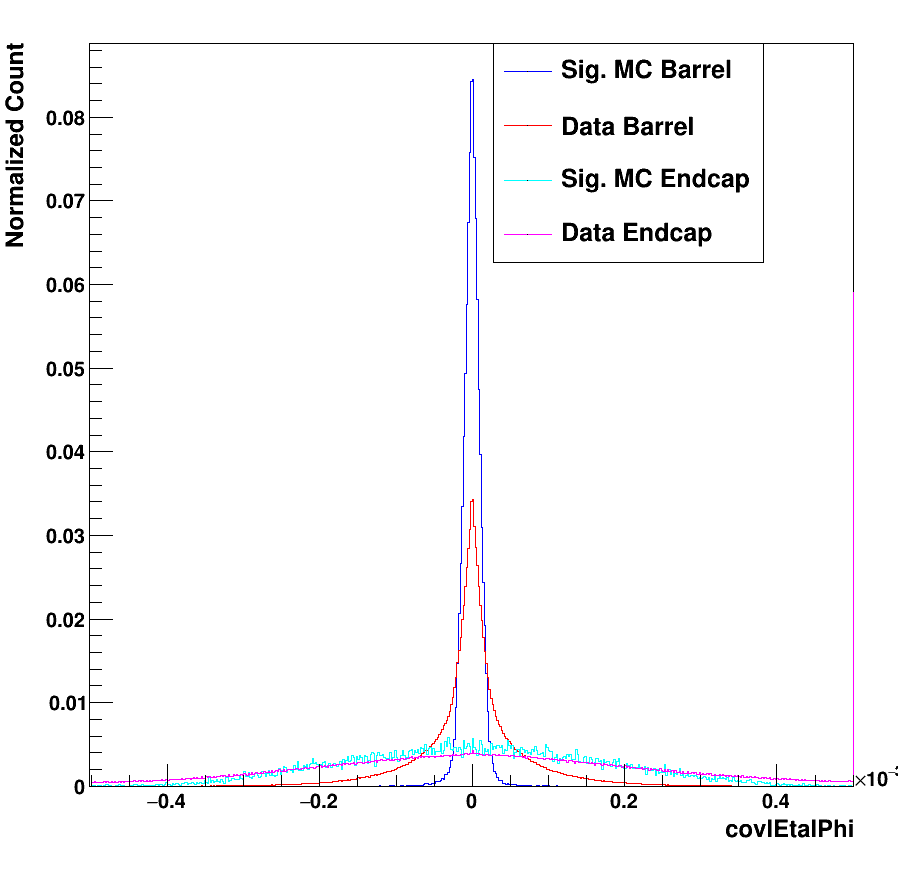
\includegraphics[width=\linewidth]{./Figures/Offline Selection Plots/DiHiggs/0715_DataMC_TrainingPlots/covIEtaIPhi.png}
		\caption{cov($i \eta i \phi$)}
		\label{DataMCVars:DiHiggs:covIetaIphi}
	\end{subfigure}
	\caption{Plots of the $\sigma_{i \eta i \eta}$ and cov($i \eta i \phi$). The signal MC is shown in dark blue for the barrel and light blue for the endcap, whereas the data (background) is shown in red for the barrel and pink for the endcap.}
	\label{fig:DiHiggs:DataMCVars3}
\end{figure}

\begin{figure}[H]
	\begin{subfigure}{0.50\linewidth}
		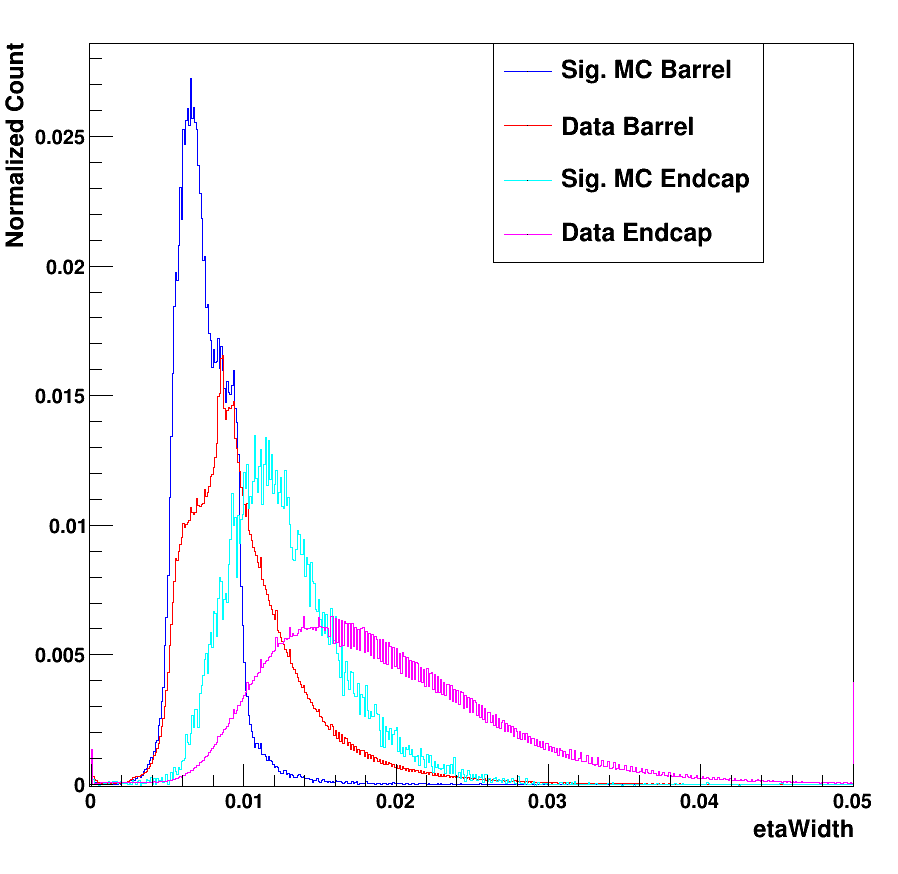
\includegraphics[width=\linewidth]{./Figures/Offline Selection Plots/DiHiggs/0715_DataMC_TrainingPlots/etaWidth.png}
		\caption{$\eta$ Width}
		\label{DataMCVars:DiHiggs:etaW}
	\end{subfigure}\hfill
	\begin{subfigure}{0.50\linewidth}
		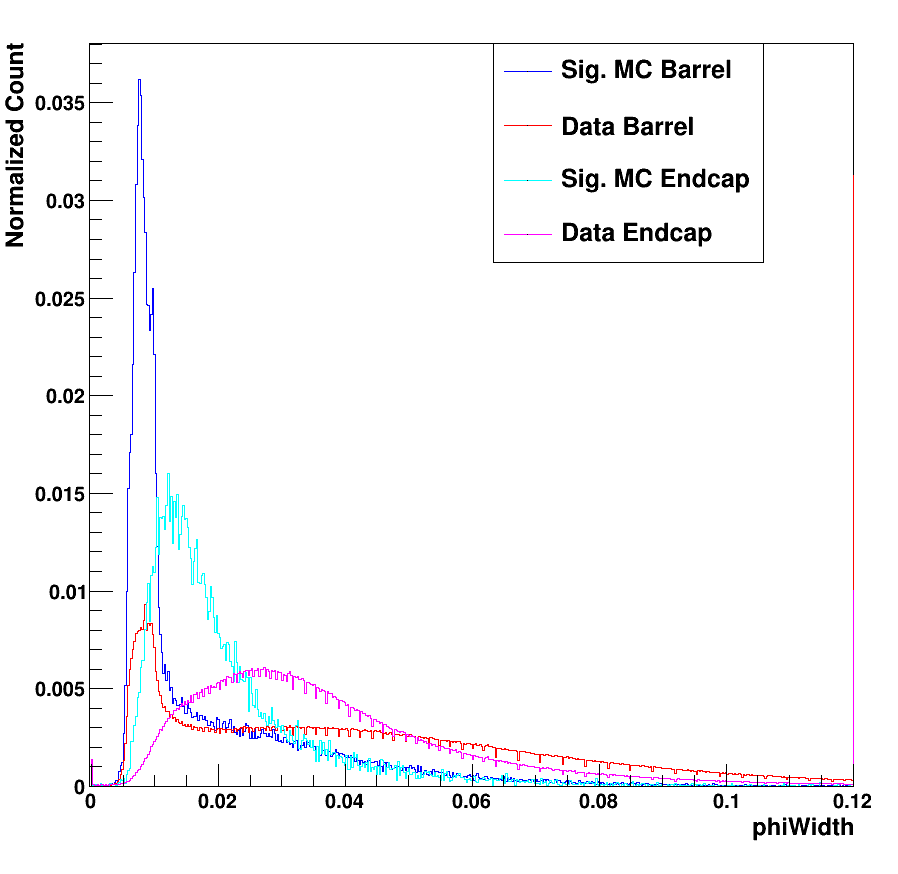
\includegraphics[width=\linewidth]{./Figures/Offline Selection Plots/DiHiggs/0715_DataMC_TrainingPlots/phiWidth.png}
		\caption{$\phi$ Width}
		\label{DataMCVars:DiHiggs:phiW}
	\end{subfigure}
	\caption{Plots of the $\eta$ and $\phi$ widths. The signal MC is shown in dark blue for the barrel and light blue for the endcap, whereas the data (background) is shown in red for the barrel and pink for the endcap.}
	\label{fig:DiHiggs:DataMCVars4}
\end{figure}

\begin{figure}[H]
	\begin{subfigure}{0.50\linewidth}
		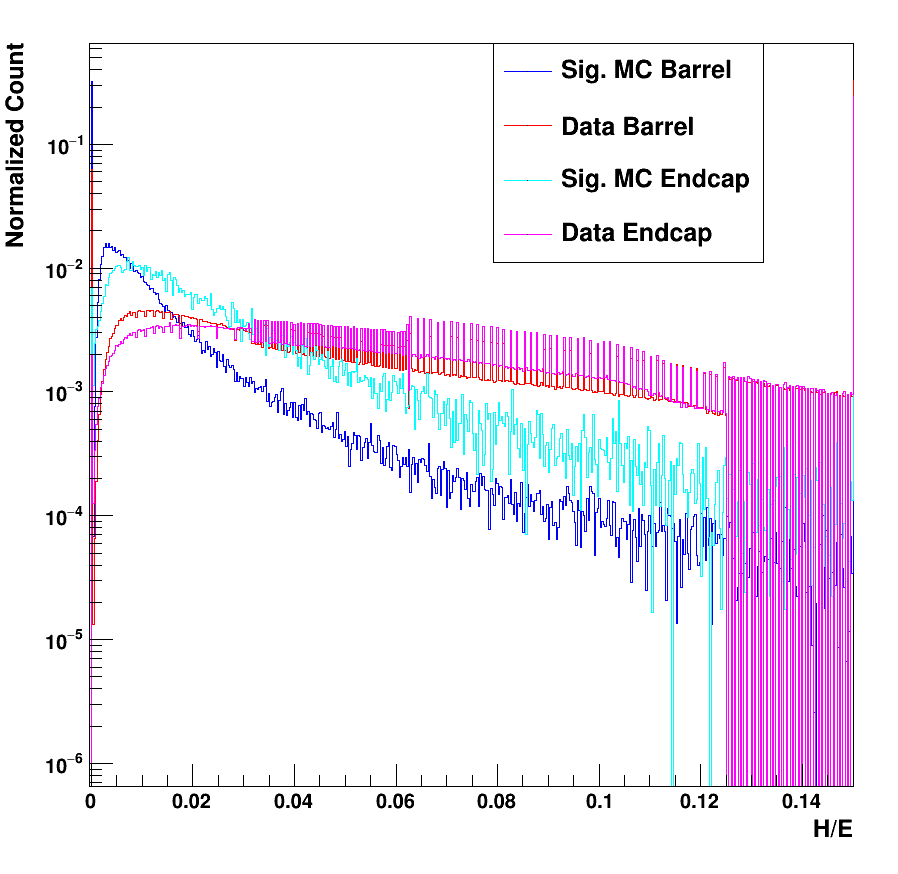
\includegraphics[width=\linewidth]{./Figures/Offline Selection Plots/DiHiggs/0715_DataMC_TrainingPlots/hadronicOverEm.png}
		\caption{H/E}
		\label{DataMCVars:DiHiggs:hoe}
	\end{subfigure}\hfill
	\begin{subfigure}{0.50\linewidth}
		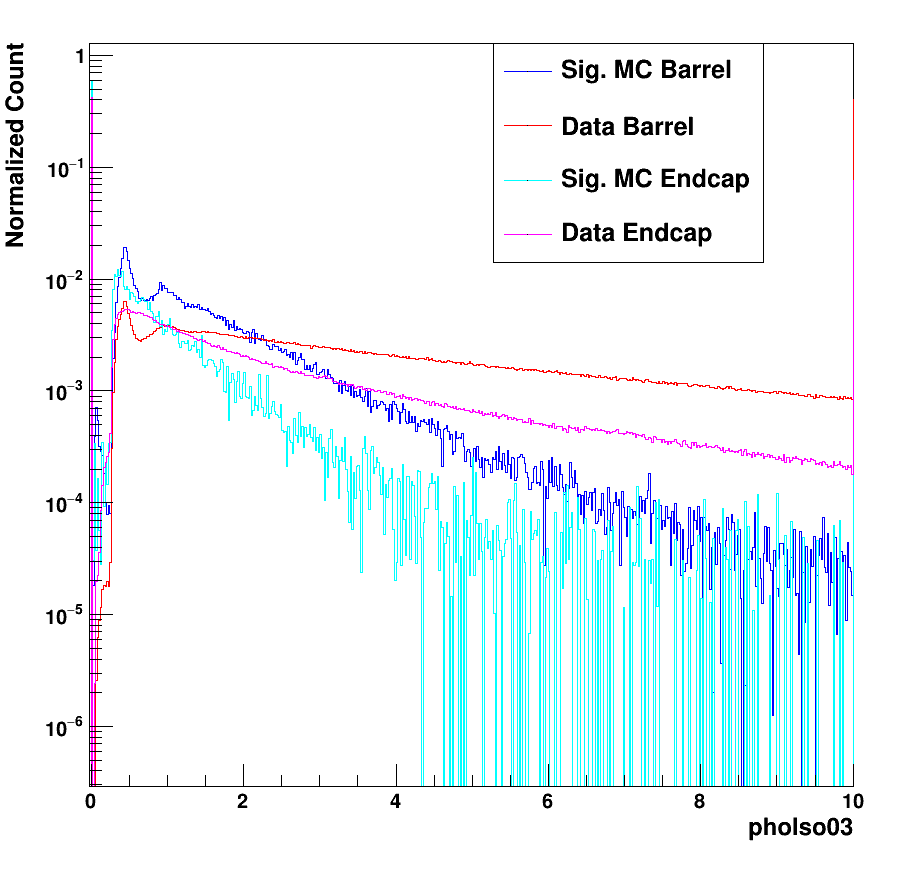
\includegraphics[width=\linewidth]{./Figures/Offline Selection Plots/DiHiggs/0715_DataMC_TrainingPlots/phoIso03.png}
		\caption{Photon Isolation}
		\label{DataMCVars:DiHiggs:phoIso}
	\end{subfigure}
	\caption{Plots of the H/E and photon isolation. The signal MC is shown in dark blue for the barrel and light blue for the endcap, whereas the data (background) is shown in red for the barrel and pink for the endcap.}
	\label{fig:DiHiggs:DataMCVars4}
\end{figure}

\begin{figure}[H]
	\begin{subfigure}{0.50\linewidth}
		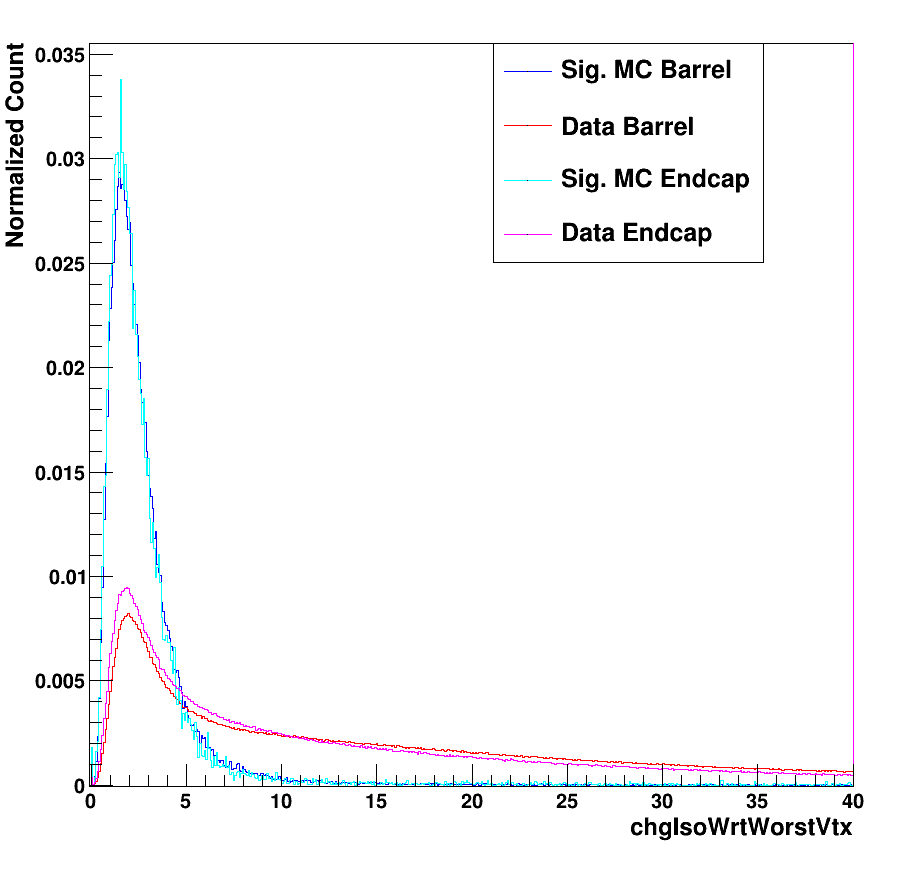
\includegraphics[width=\linewidth]{./Figures/Offline Selection Plots/DiHiggs/0715_DataMC_TrainingPlots/chgIsoWrtWorstVtx.png}
		\caption{Chg. Iso. W.r.t. Worst Vertex}
		\label{DataMCVars:DiHiggs:chgIsoWorst}
	\end{subfigure}\hfill
	\begin{subfigure}{0.50\linewidth}
		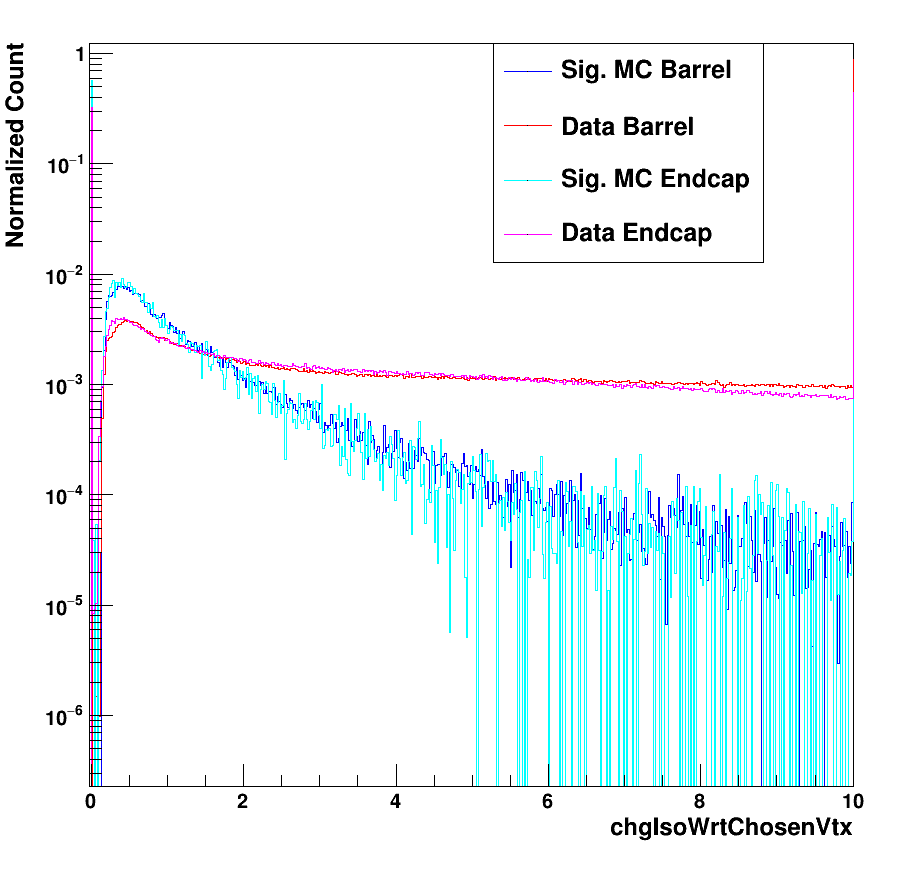
\includegraphics[width=\linewidth]{./Figures/Offline Selection Plots/DiHiggs/0715_DataMC_TrainingPlots/chgIsoWrtChosenVtx.png}
		\caption{Chg. Iso. W.r.t. Chosen Vertex}
		\label{DataMCVars:DiHiggs:chgIsoChosen}
	\end{subfigure}
	\caption{Plots of the charged isolations with respect to the worst and chosen vertices. The signal MC is shown in dark blue for the barrel and light blue for the endcap, whereas the data (background) is shown in red for the barrel and pink for the endcap.}
	\label{fig:DiHiggs:DataMCVars5}
\end{figure}

\begin{figure}[H]
	\begin{subfigure}{0.50\linewidth}
		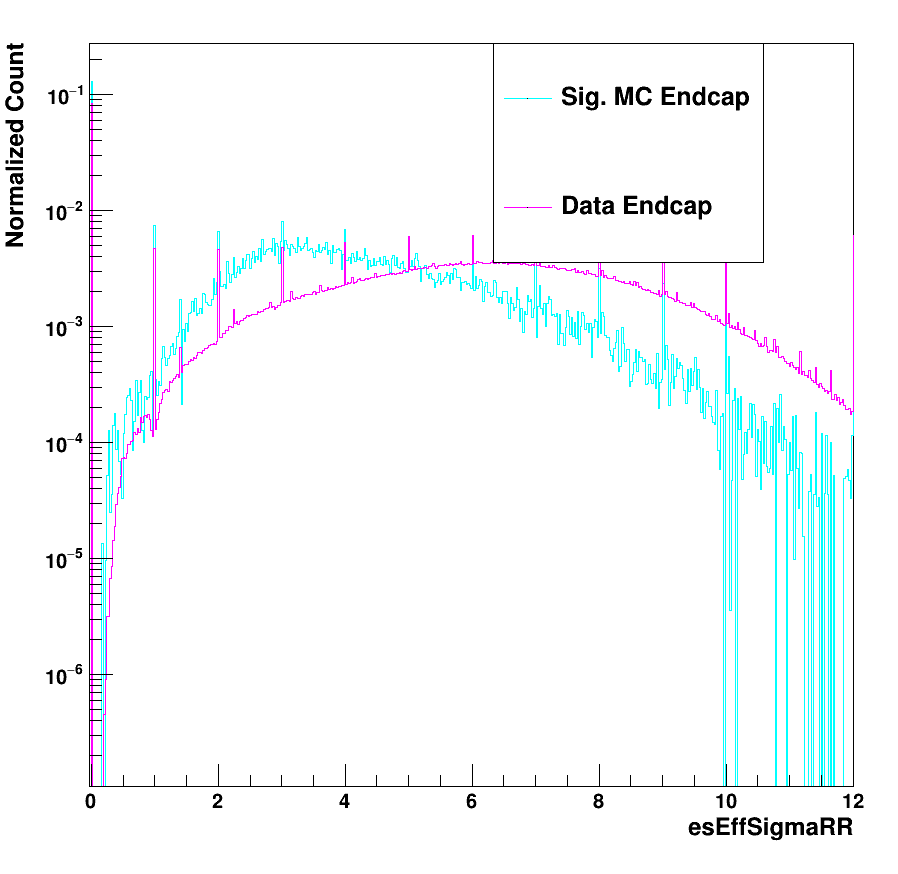
\includegraphics[width=\linewidth]{./Figures/Offline Selection Plots/DiHiggs/0715_DataMC_TrainingPlots/esEffSigmaRR.png}
		\caption{ES Eff. Sigma RR}
		\label{DataMCVars:DiHiggs:esEffSigmaRR}
	\end{subfigure}\hfill
	\begin{subfigure}{0.50\linewidth}
		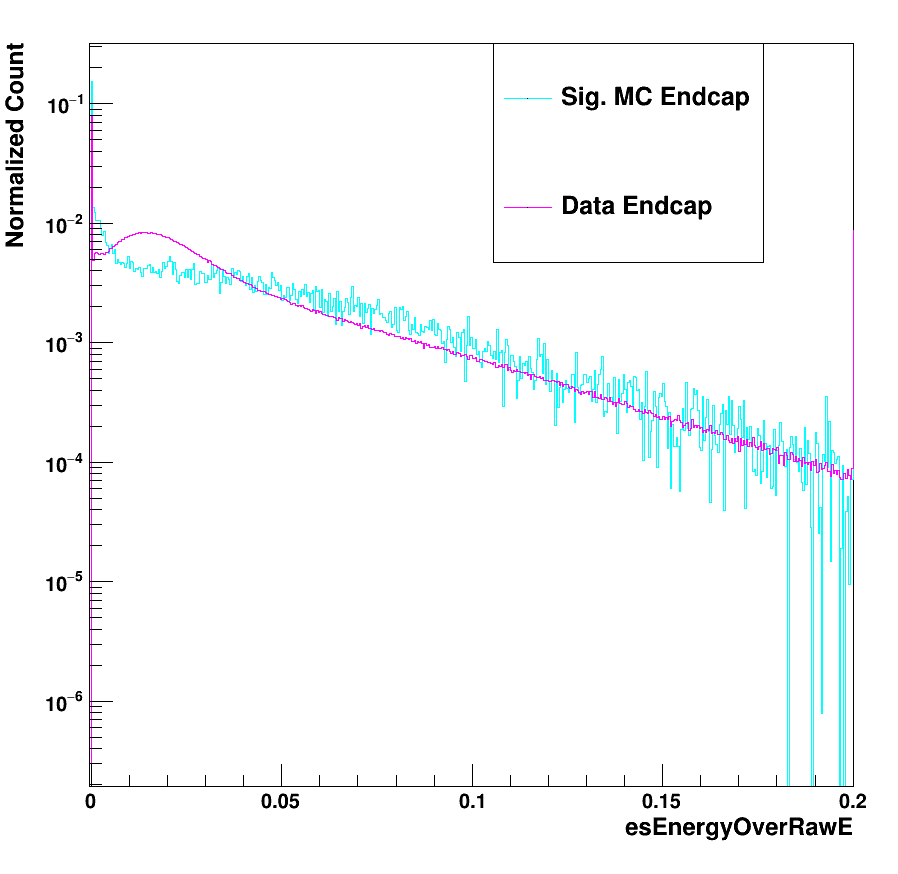
\includegraphics[width=\linewidth]{./Figures/Offline Selection Plots/DiHiggs/0715_DataMC_TrainingPlots/esEnergyOverRawE.png}
		\caption{ES Energy over Raw E}
		\label{DataMCVars:DiHiggs:esEnergyOverRawE}
	\end{subfigure}
	\caption{Plots of the ES Eff. Sigma RR and ES Energy over Raw E. The signal MC is shown in dark blue for the barrel and light blue for the endcap, whereas the data (background) is shown in red for the barrel and pink for the endcap.}
	\label{fig:DiHiggs:DataMCVars6}
\end{figure}

\subsection{Determination of Loose Single Photon MVA Cuts for $HH \rightarrow b \bar{b} \gamma \gamma$}\label{sec:DiHiggsSinglePhoCuts}

Given the difference in the resulting output BDT score distributions, the loose single photon cuts must be reexamined for the DiHiggs sample. As previously mentioned, this readjustment of the cuts is a relatively straightforward process. Again, the general goal was to achieve an approximately 98\% signal efficiency. Relative to the single H cuts, both the $\gamma$ + Jet and Data/MC cuts are numerically tighter. The chosen cuts yielded a total signal efficiency of 97.35\% and a corresponding data acceptance of 14.7\%. While both of these values are fractionally lower than that of the single Higgs, there is still ample signal efficiency with which to realize the gains from the trigger level. On the other hand, the preselection yields a signal efficiency of 67.78\%, which is considerably lower than that of the single Higgs. 
\begin{figure}[H]
	\begin{subfigure}{0.50\linewidth}
		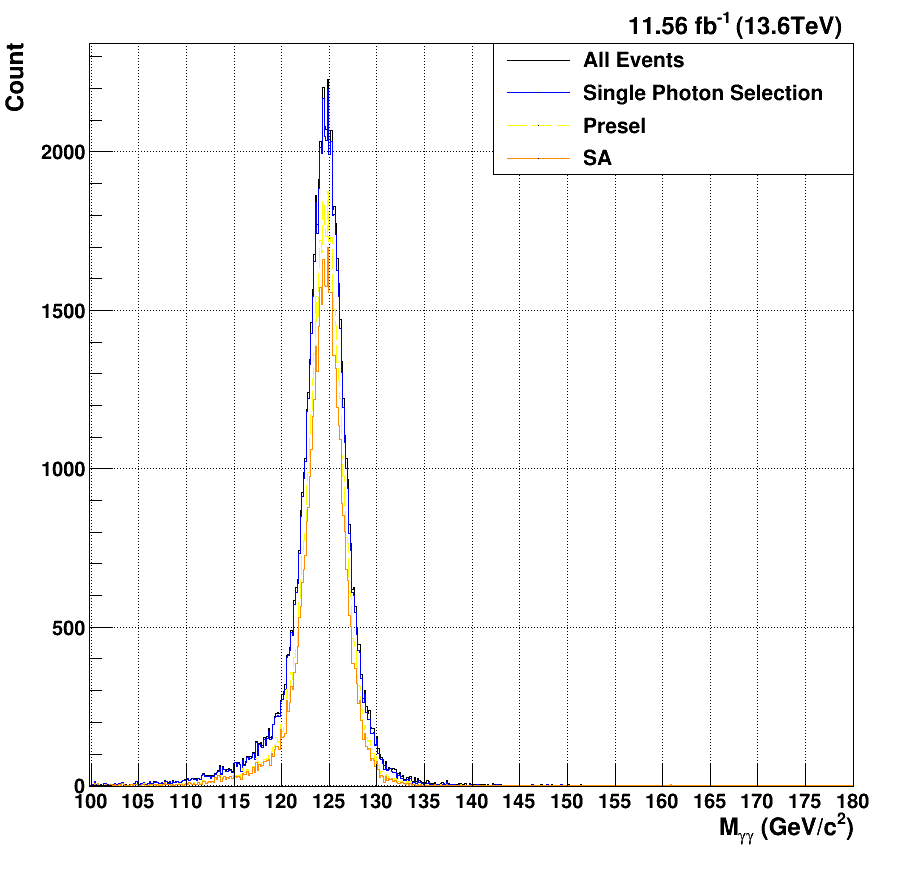
\includegraphics[width=\linewidth]{./Figures/Offline Selection Plots/DiHiggs/0715_SinglePhoOfflineCuts_SingleSquarePlots/hggMass_All_Sig.png}
		\caption{Signal MC $M_{\gamma \gamma}$}
		\label{SinglePhoCuts:DiHiggs:MggSig}
	\end{subfigure}\hfill
	\begin{subfigure}{0.50\linewidth}
		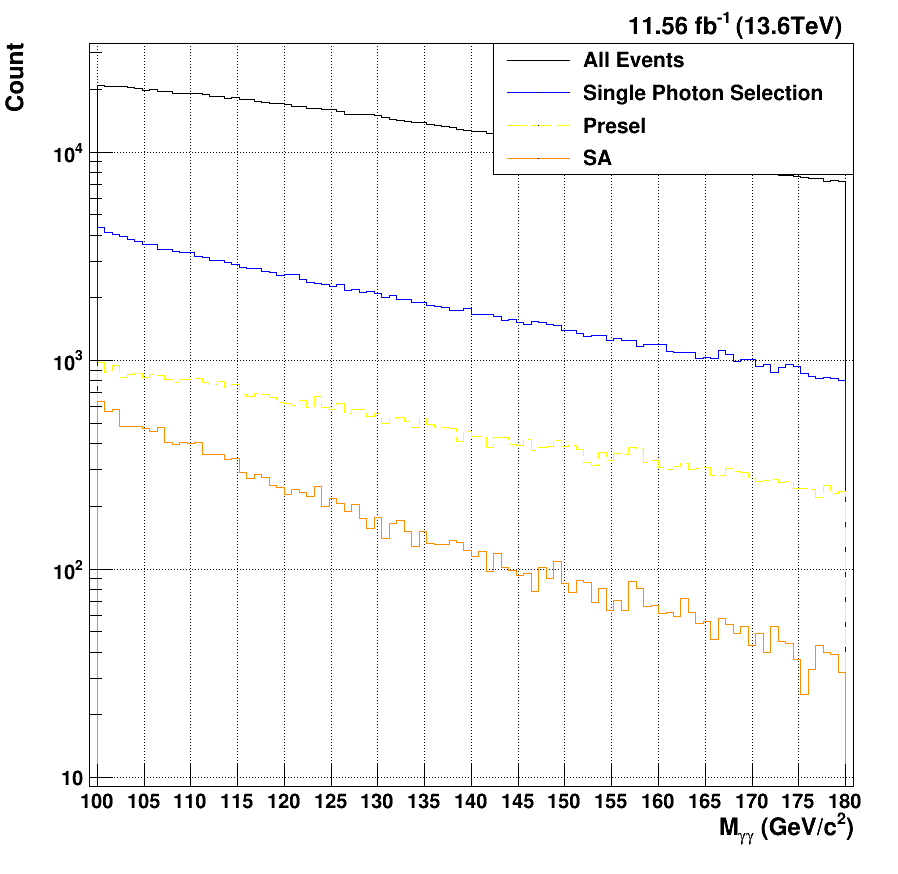
\includegraphics[width=\linewidth]{./Figures/Offline Selection Plots/DiHiggs/0715_SinglePhoOfflineCuts_SingleSquarePlots/hggMass_All_Bkg.png}
		\caption{Data $M_{\gamma \gamma}$}
		\label{SinglePhoCuts:DiHiggs:MggBkg}
	\end{subfigure}
	\caption{Acceptance of the MVA-HLT (blue) vs. the current standard diphoton HLT (green) for $M_{\gamma \gamma}$}
	\label{fig:DiHiggs:SinglePhoCutsMgg}
\end{figure}


\begin{figure}[H]
	\begin{subfigure}{0.50\linewidth}
		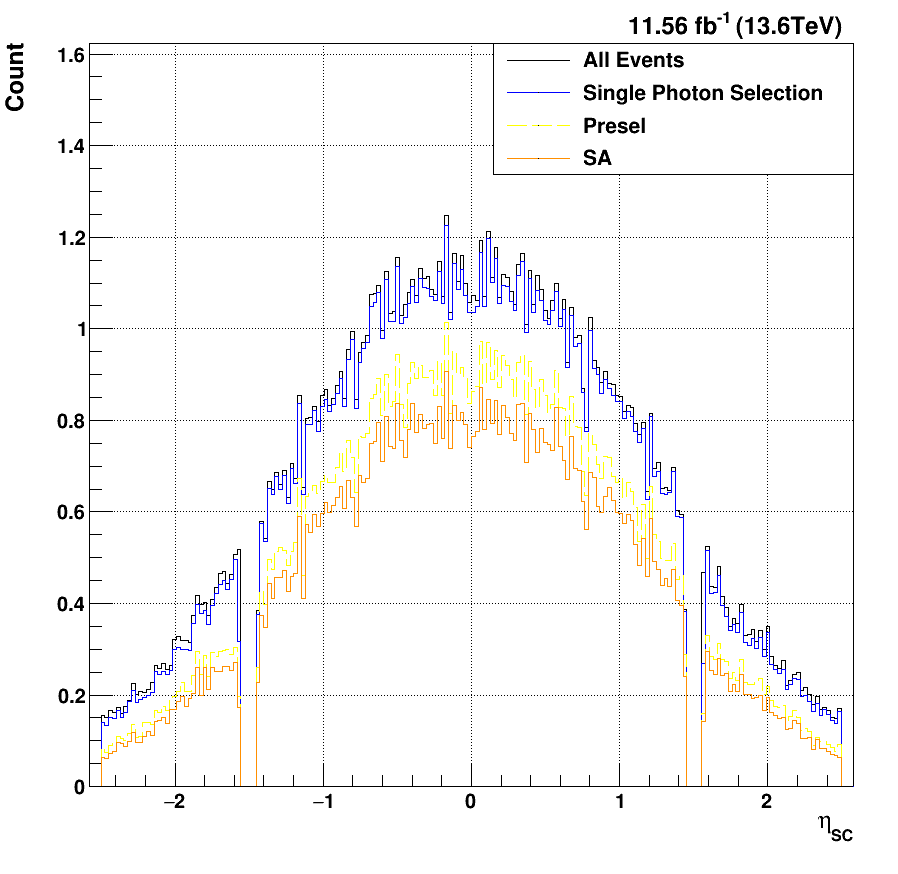
\includegraphics[width=\linewidth]{./Figures/Offline Selection Plots/DiHiggs/0715_SinglePhoOfflineCuts_SingleSquarePlots/scEta_All_Sig.png}
		\caption{Signal MC $\eta_{SC}$}
		\label{SinglePhoCuts:DiHiggs:EtaSig}
	\end{subfigure}\hfill
	\begin{subfigure}{0.50\linewidth}
		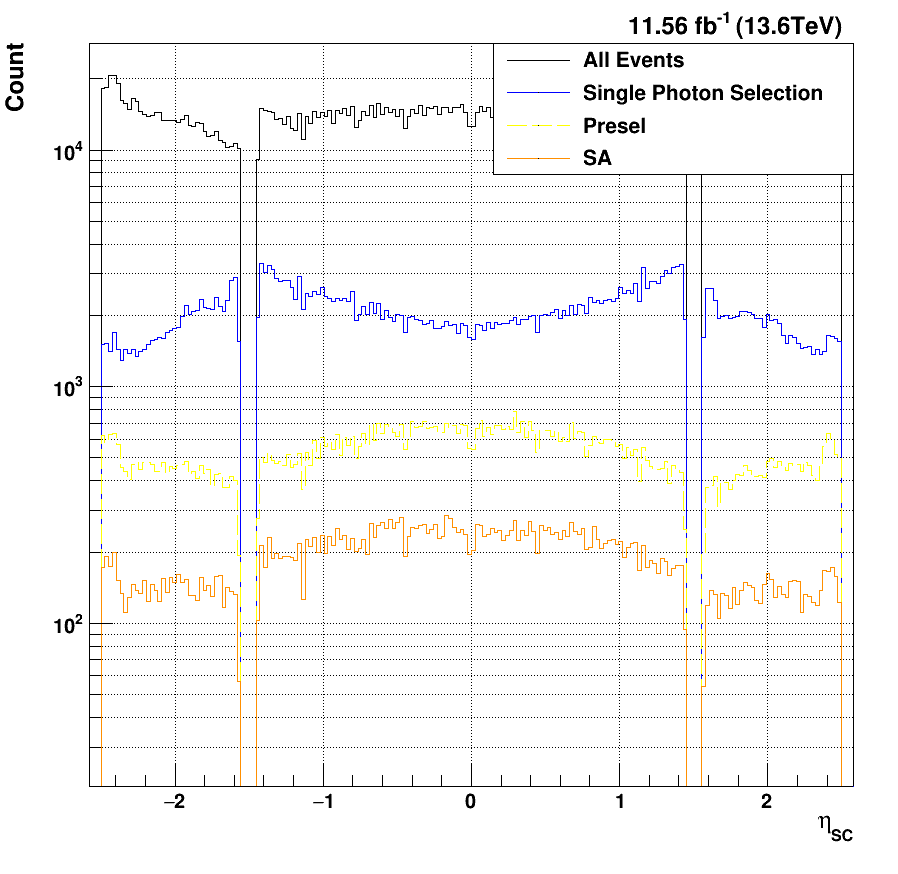
\includegraphics[width=\linewidth]{./Figures/Offline Selection Plots/DiHiggs/0715_SinglePhoOfflineCuts_SingleSquarePlots/scEta_All_Bkg.png}
		\caption{Data $\eta_{SC}$}
		\label{SinglePhoCuts:DiHiggs:EtaBkg}
	\end{subfigure}
	\caption{Acceptance of the MVA-HLT (blue) vs. the current standard diphoton HLT (green) for $\eta_{SC}$}
	\label{fig:DiHiggs:SinglePhoCutsEta}
\end{figure}

Relative to the singleH selection, the DiHiggs data acceptance is relatively unchanged. Of course, given the very high signal efficiency of this selection, there is little effect on the signal acceptance. A relevant kinematic difference can be seen, however; the DiHiggs signal MC tends to be far more central in the barrel, with very little extending into the endcap. This highlights, again, why retraining both the single photon Data/MC BDT and the diphoton BDT is so crucial for this sample.

\begin{figure}[H]
	\begin{subfigure}{0.50\linewidth}
		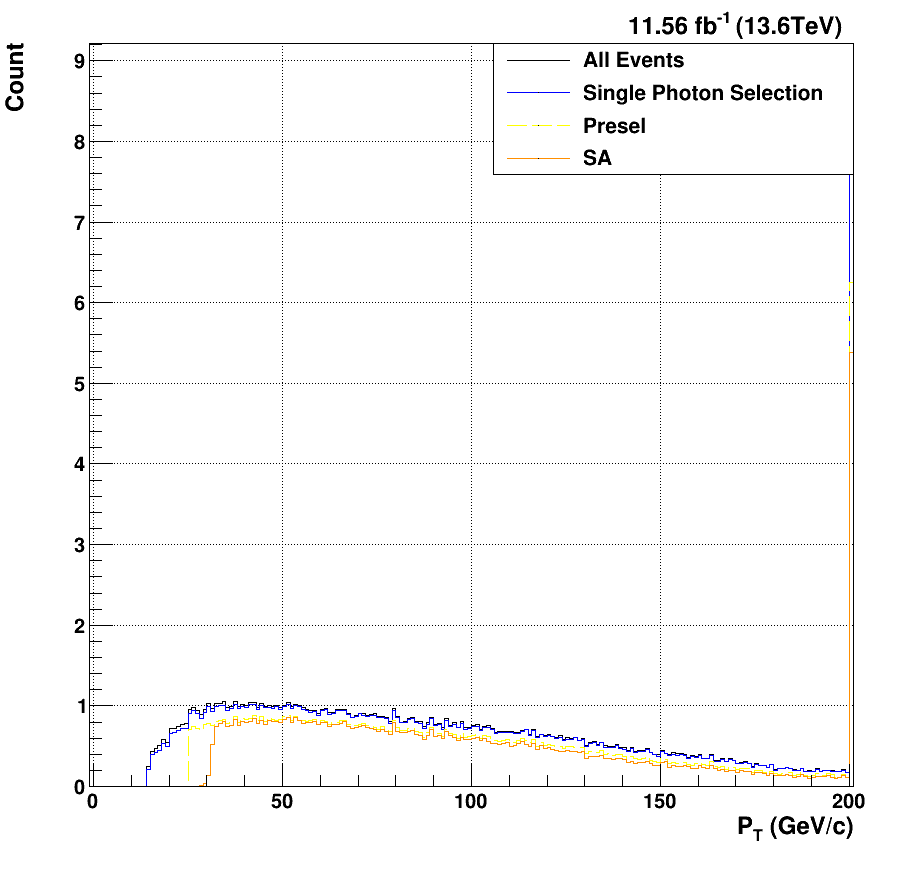
\includegraphics[width=\linewidth]{./Figures/Offline Selection Plots/DiHiggs/0715_SinglePhoOfflineCuts_SingleSquarePlots/pt_All_Sig.png}
		\caption{Signal MC $p_{T}$}
		\label{SinglePhoCuts:DiHiggs:PtSig}
	\end{subfigure}\hfill
	\begin{subfigure}{0.50\linewidth}
		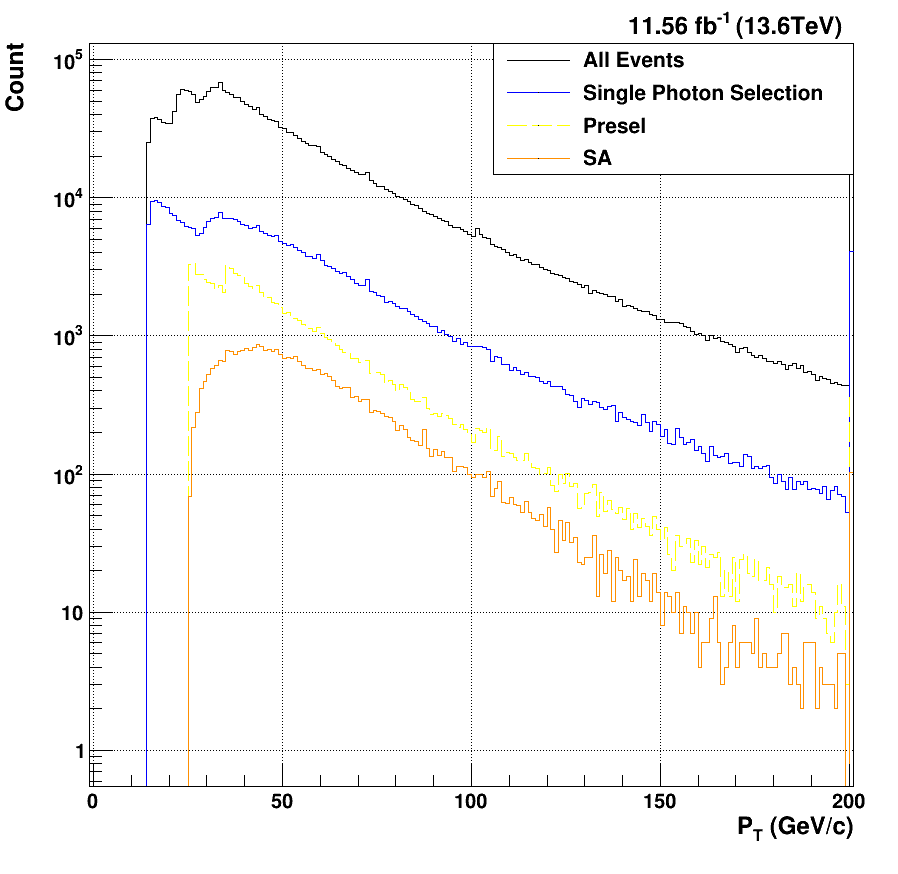
\includegraphics[width=\linewidth]{./Figures/Offline Selection Plots/DiHiggs/0715_SinglePhoOfflineCuts_SingleSquarePlots/pt_All_Bkg.png}
		\caption{Data $p_{T}$}
		\label{SinglePhoCuts:DiHiggs:PtBkg}
	\end{subfigure}
	\caption{Acceptance of the MVA-HLT (blue) vs. the current standard diphoton HLT (green) for $p_{T}$}
	\label{fig:DiHiggs:SinglePhoCutsPt}
\end{figure}

The scale of the accepted $p_T$ values is quite skewed by the very large bin content of the overflow bin (above 200 GeV/c). This points to another important kinematic difference -- given the more central photon distribution in $\eta_{SC}$, the photon candidates tend to have higher $p_T$ values on average. 

\subsection{Creation of Diphoton BDT for $HH \rightarrow b \bar{b} \gamma \gamma$}

The final step is to consider the recreation of the diphoton BDT for the DiHiggs process. It will be shown in figures \ref{fig:DiHiggs:DiphoVars1}-\ref{fig:DiHiggs:DiphoVars6} that both the kinematic variables and the input BDT score distributions are significantly different relative to the single Higgs.
\begin{figure}[H]
	\begin{subfigure}{0.50\linewidth}
		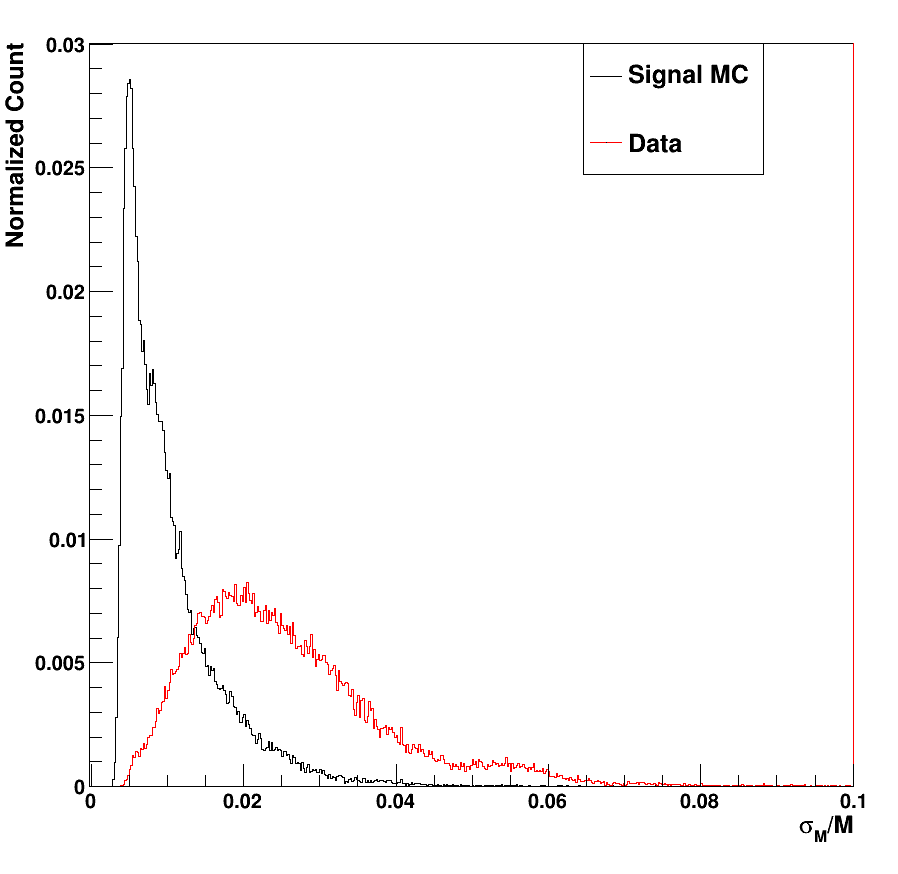
\includegraphics[width=\linewidth]{./Figures/Offline Selection Plots/DiHiggs/0715_DiphotonBDT_TrainingPlots/sigMovrM.png}
		\caption{$\sigma(M_{\gamma \gamma})/M_{\gamma \gamma}$}
		\label{DiphoVars:DiHiggs:sigmaMovrM}
	\end{subfigure}\hfill
	\begin{subfigure}{0.50\linewidth}
		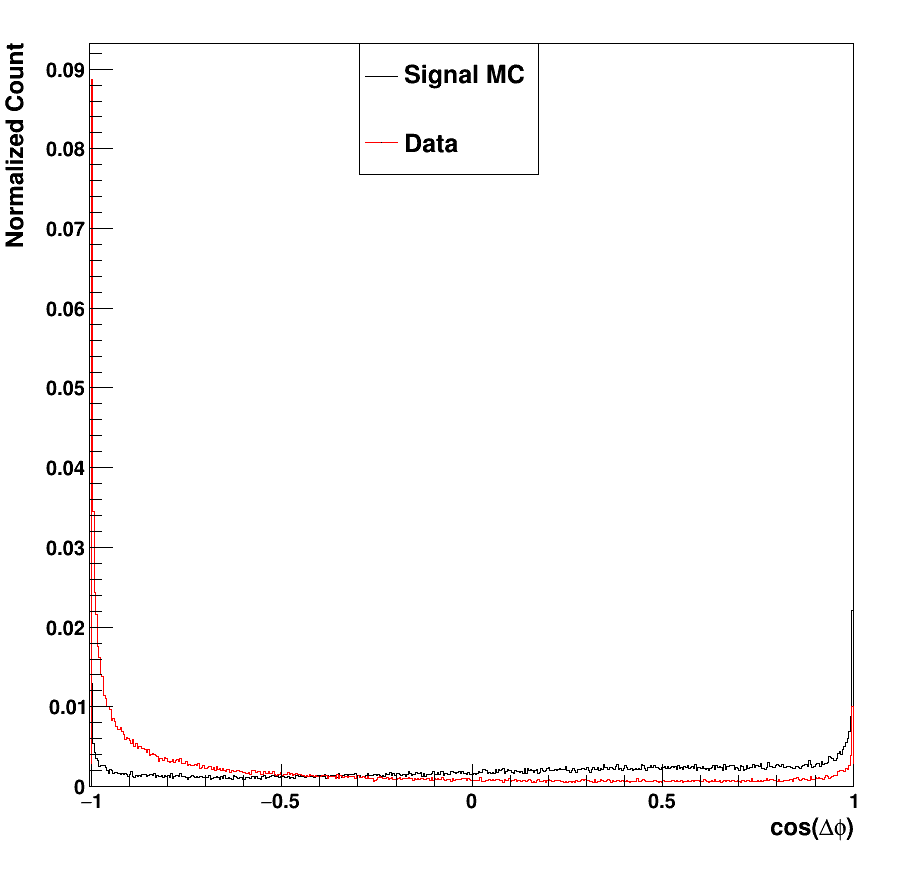
\includegraphics[width=\linewidth]{./Figures/Offline Selection Plots/DiHiggs/0715_DiphotonBDT_TrainingPlots/cosDPhi.png}
		\caption{cos($\Delta \phi$)}
		\label{DiphoVars:DiHiggs:cosDPhi}
	\end{subfigure}
	\caption{The two per-event diphoton input variables,$\sigma(M_{\gamma \gamma})/M_{\gamma \gamma}$ and cos($\Delta \phi$). The signal MC is in black, whereas the data events are in red.}
	\label{fig:DiHiggs:DiphoVars1}
\end{figure}

While the $\sigma(M_{\gamma \gamma})/M_{\gamma \gamma}$ disributions are relatively similar to their single Higgs counterparts, there are minor differences in the cos($\Delta \phi$). The single Higgs for both the data and signal MC was strongly peaked at -1, with a very similar shape for both samples. In the DiHiggs, however, there is far better separation between the signal and background; the data is still relatively well clustered at -1, but the signal MC has a sloped shape favoring higher values (especially increasing approaching 1). This, again, is due to the kinematics of the DiHiggs production. Cos($\Delta \phi$) = -1 corresponds to a $\Delta \phi = \pi$, whereas Cos($\Delta \phi$) = 1 corresponds to a $\Delta \phi = 0$. As expected, then, the DiHiggs signal is more likely to have a lower separation in $\phi$. So, the discrimination power of this variable should have increased relative to the single Higgs.

\begin{figure}[H]
	\begin{subfigure}{0.50\linewidth}
		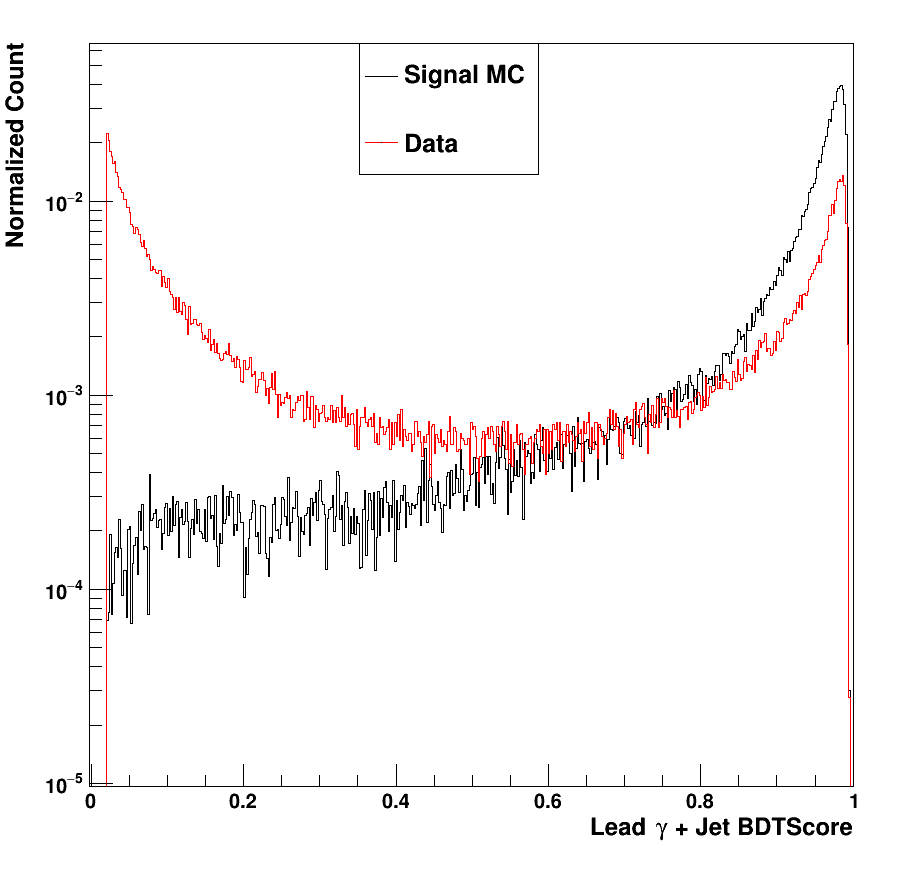
\includegraphics[width=\linewidth]{./Figures/Offline Selection Plots/DiHiggs/0715_DiphotonBDT_TrainingPlots/leadGJetXGBScore.png}
		\caption{Lead $\gamma$ + Jet BDT Score}
		\label{DiphoVars:DiHiggs:leadGJetXGBScore}
	\end{subfigure}\hfill
	\begin{subfigure}{0.50\linewidth}
		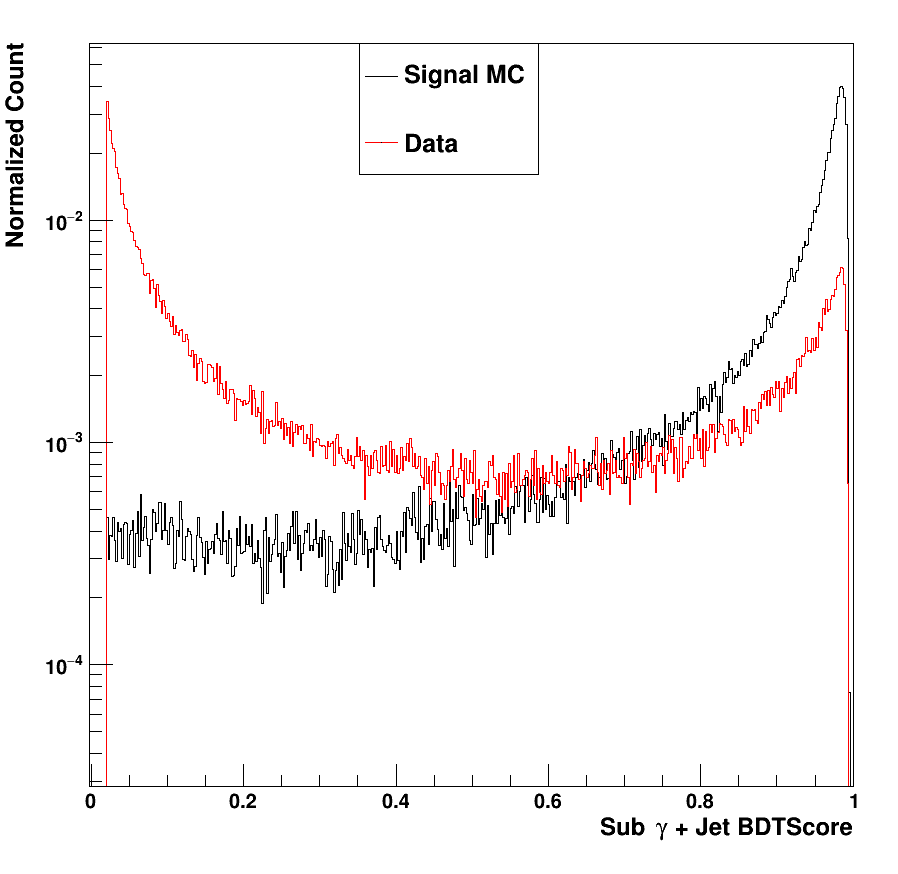
\includegraphics[width=\linewidth]{./Figures/Offline Selection Plots/DiHiggs/0715_DiphotonBDT_TrainingPlots/subGJetXGBScore.png}
		\caption{Sub $\gamma$ + Jet BDT Score}
		\label{DiphoVars:DiHiggs:subGJetXGBScore}
	\end{subfigure}
	\caption{The lead and sublead $\gamma$ + Jet XGBoost BDT scores. The signal MC is in black, whereas the data events are in red.}
	\label{fig:DiHiggs:DiphoVars2}
\end{figure}

Next, there are clear differences in the $\gamma$ + Jet BDT score distributions for the DiHiggs. The signal MC, surprisingly, has a relatively similar distribution in scores. The score peaks strongly at 1 for the signal in both the lead and sublead photon candidate. The data, however, has moved closer to 0. Especially in the sublead photon candidate, the peak near 0 is taller than the peak near 1. In the single Higgs, the two peaks were of a more similar size. Even though this $\gamma$ + Jet BDT was mot retrained, it appears to perform better on separating DiHiggs signal MC from data.

\begin{figure}[H]
	\begin{subfigure}{0.50\linewidth}
		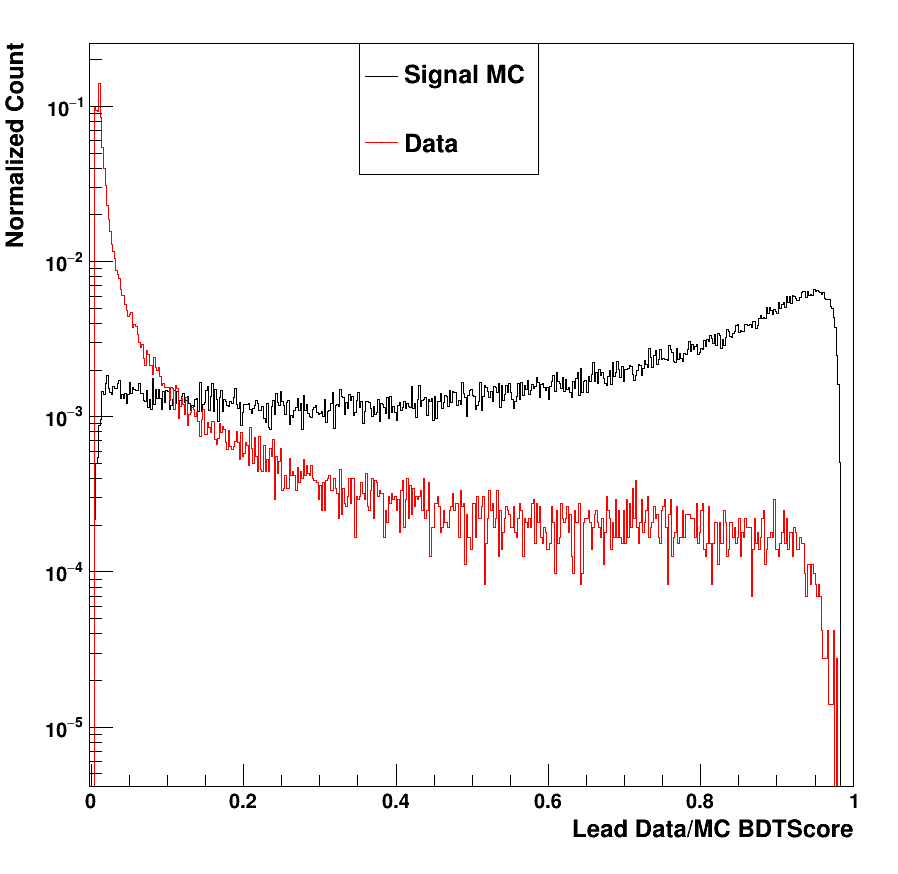
\includegraphics[width=\linewidth]{./Figures/Offline Selection Plots/DiHiggs/0715_DiphotonBDT_TrainingPlots/leadDataMCXGBScore.png}
		\caption{Lead Data/MC BDT Score}
		\label{DiphoVars:DiHiggs:leadDataMCXGBScore}
	\end{subfigure}\hfill
	\begin{subfigure}{0.50\linewidth}
		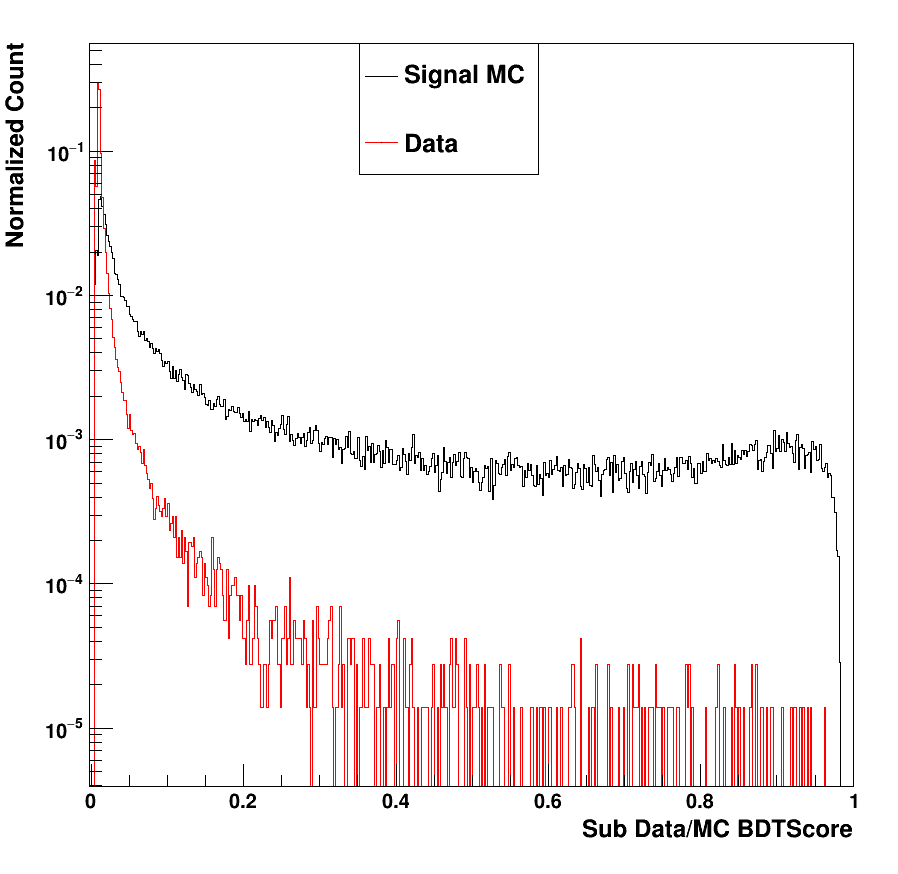
\includegraphics[width=\linewidth]{./Figures/Offline Selection Plots/DiHiggs/0715_DiphotonBDT_TrainingPlots/subDataMCXGBScore.png}
		\caption{Sub Data/MC BDT Score}
		\label{DiphoVars:DiHiggs:subDataMCXGBScore}
	\end{subfigure}
	\caption{The lead and sublead Data/MC XGBoost BDT scores. The signal MC is in black, whereas the data events are in red.}
	\label{fig:DiHiggs:DiphoVars3}
\end{figure}

The single photon Data/MC BDT scores are quite well-separated for the lead photon, perhaps moreso than they were for the single Higgs sample. Clearly, as well, the sublead scores for the data are very well-placed near 0. Again, in conjunction with the $\gamma$ + Jet scores shown in figure \ref{fig:DiHiggs:DiphoVars2}, these data/MC BDT scores will have strong discrimination power.

\begin{figure}[H]
	\begin{subfigure}{0.50\linewidth}
		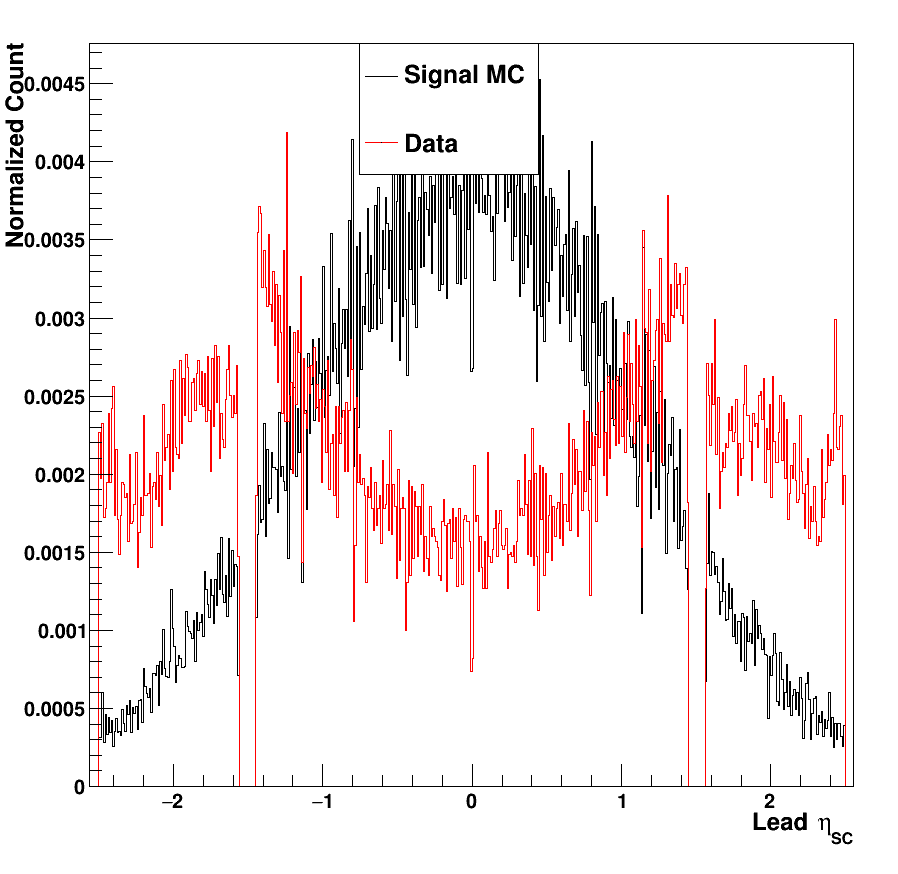
\includegraphics[width=\linewidth]{./Figures/Offline Selection Plots/DiHiggs/0715_DiphotonBDT_TrainingPlots/leadScEta.png}
		\caption{Lead $\eta_{SC}$}
		\label{DiphoVars:DiHiggs:leadScEta}
	\end{subfigure}\hfill
	\begin{subfigure}{0.50\linewidth}
		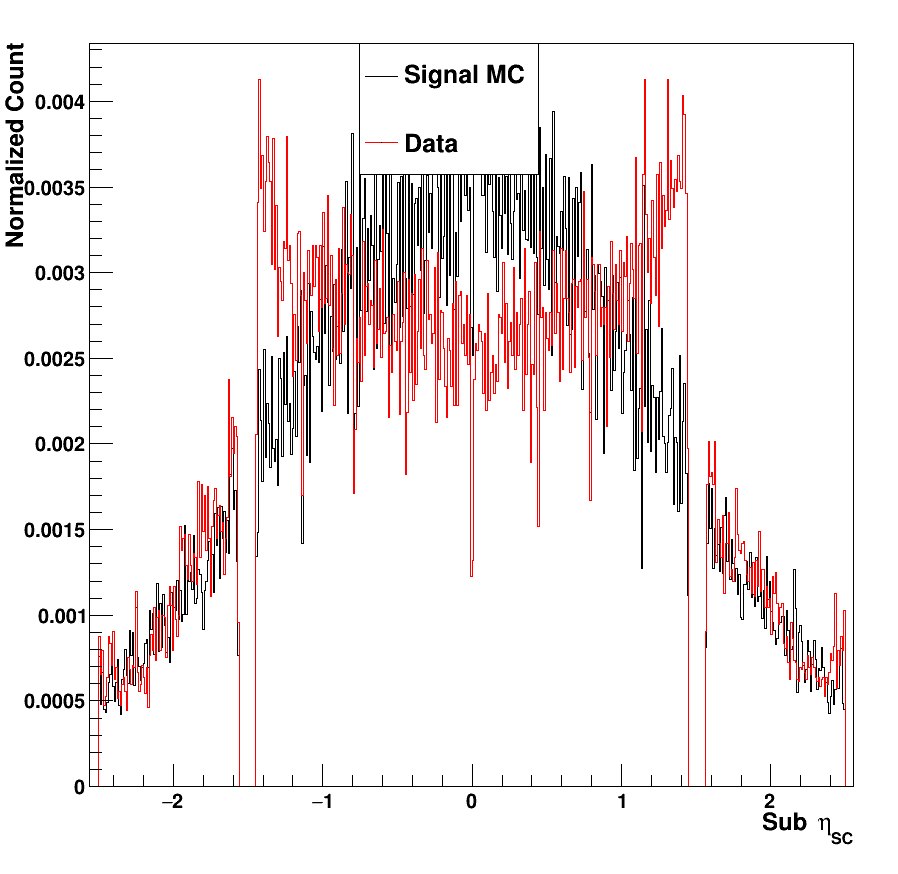
\includegraphics[width=\linewidth]{./Figures/Offline Selection Plots/DiHiggs/0715_DiphotonBDT_TrainingPlots/subScEta.png}
		\caption{Sub $\eta_{SC}$}
		\label{DiphoVars:DiHiggs:subScEta}
	\end{subfigure}
	\caption{The lead and sublead $\eta_{SC}$. The signal MC is in black, whereas the data events are in red.}
	\label{fig:DiHiggs:DiphoVars4}
\end{figure}

As mentioned for the selection of the single photon cuts, the $\eta_{SC}$ distributions for the diHiggs samples are more separated than those of the single Higgs. Especially in the lead photon candidate, there is very little data in the center of the barrel, while the signal MC sees its strongest peak in this region. The endcap shapes are rather different for the lead photon, but much more similar for the sublead photon. Again, due to the difference in kinematics relative to the single Higgs, these differences are to be expected.

\begin{figure}[H]
	\begin{subfigure}{0.50\linewidth}
		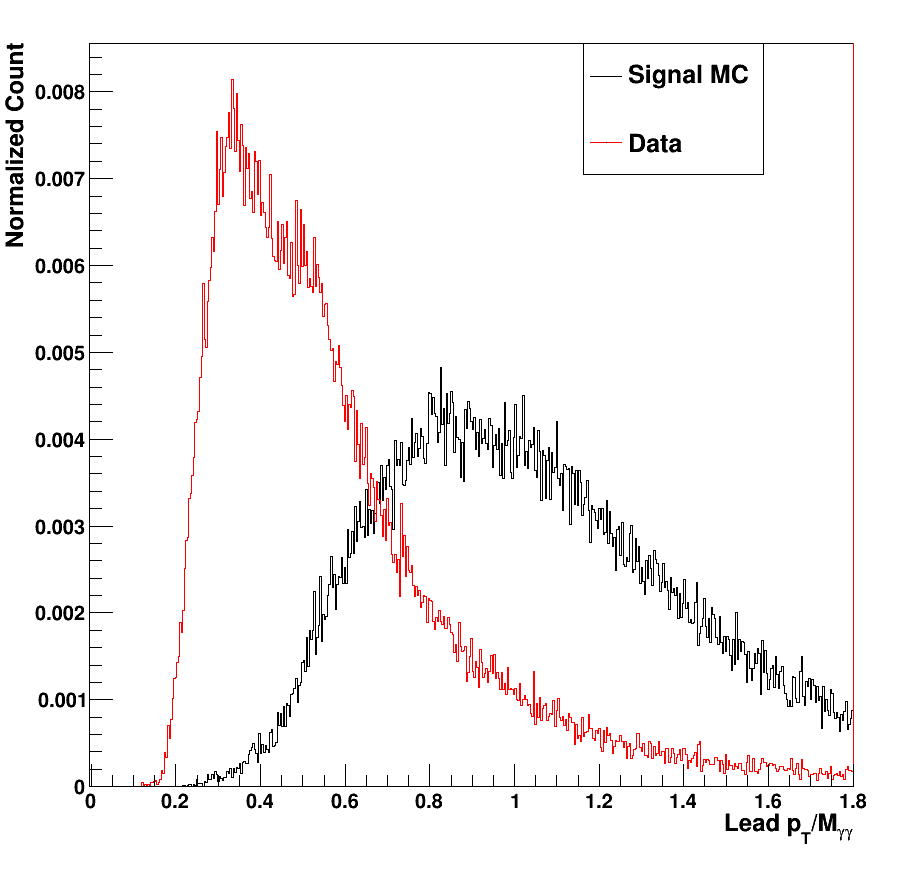
\includegraphics[width=\linewidth]{./Figures/Offline Selection Plots/DiHiggs/0715_DiphotonBDT_TrainingPlots/leadPtOvrM.png}
		\caption{Lead $p_T/M_{\gamma \gamma}$}
		\label{DiphoVars:DiHiggs:leadPtM}
	\end{subfigure}\hfill
	\begin{subfigure}{0.50\linewidth}
		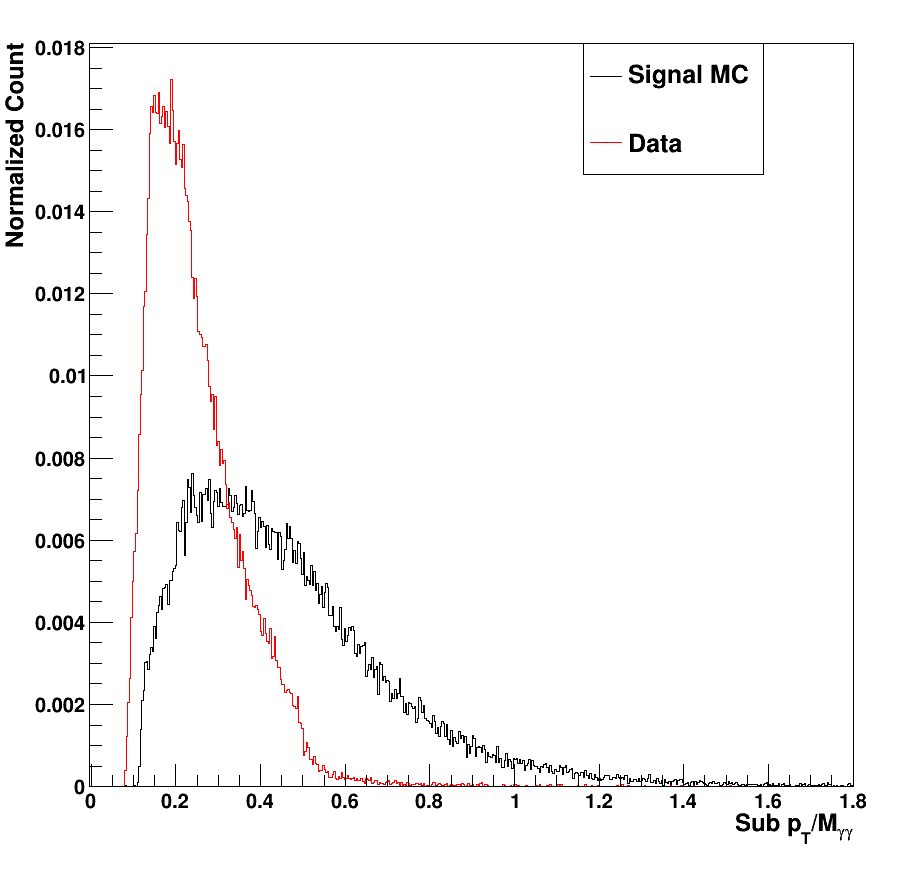
\includegraphics[width=\linewidth]{./Figures/Offline Selection Plots/DiHiggs/0715_DiphotonBDT_TrainingPlots/subPtOvrM.png}
		\caption{Sub $p_T/M_{\gamma \gamma}$}
		\label{DiphoVars:DiHiggs:subPtM}
	\end{subfigure}
	\caption{The lead and sublead $p_T/M_{\gamma \gamma}$. The signal MC is in black, whereas the data events are in red.}
	\label{fig:DiHiggs:DiphoVars5}
\end{figure}

While the separation between the signal and background for both lead and sublead $p_T/M_{\gamma \gamma}$ is still quite good (as seen in figure \ref{fig:DiHiggs:DiphoVars5}), the distributions for the signal MC are quite different than those for the single Higgs. Specifically, the values tend to be, on average, a bit higher for both the lead and sublead. Additionally, the spread of the values for the signal MC is quite a bit higher, which likely reduces the discrimination power of the $p_T/M_{\gamma \gamma}$ for the diHiggs samples.

\begin{figure}[H]
	\begin{subfigure}{0.50\linewidth}
		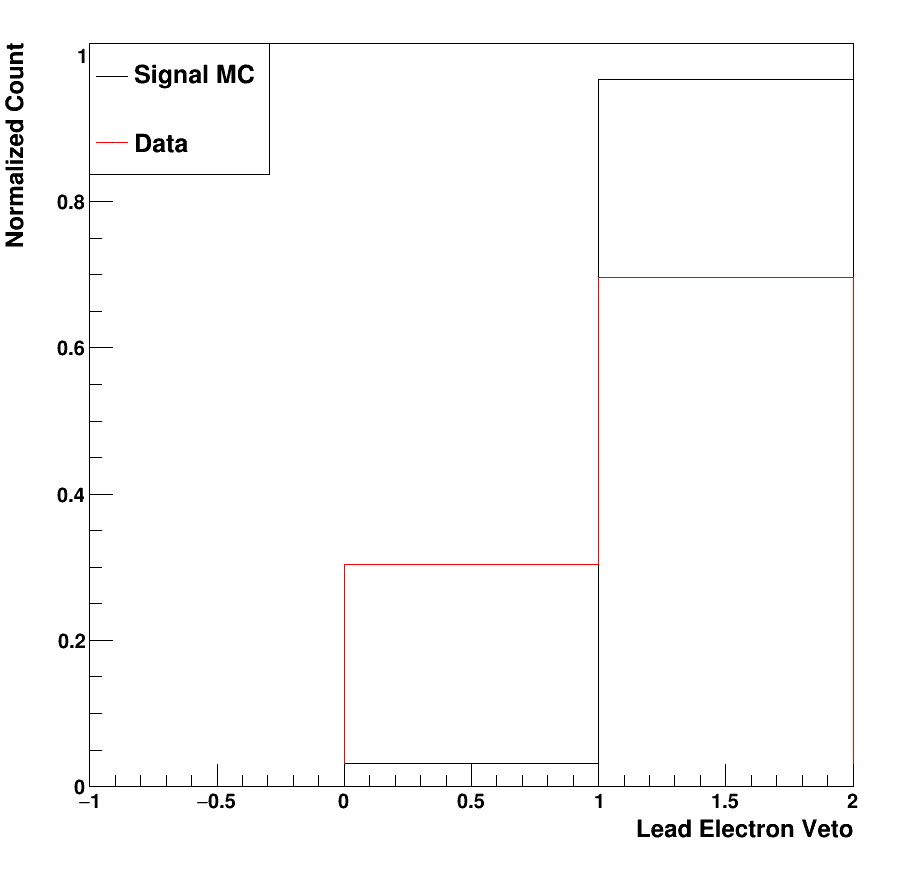
\includegraphics[width=\linewidth]{./Figures/Offline Selection Plots/DiHiggs/0715_DiphotonBDT_TrainingPlots/leadElectronVeto.png}
		\caption{Lead Electron Veto}
		\label{DiphoVars:DiHiggs:leadElectronVeto}
	\end{subfigure}\hfill
	\begin{subfigure}{0.50\linewidth}
		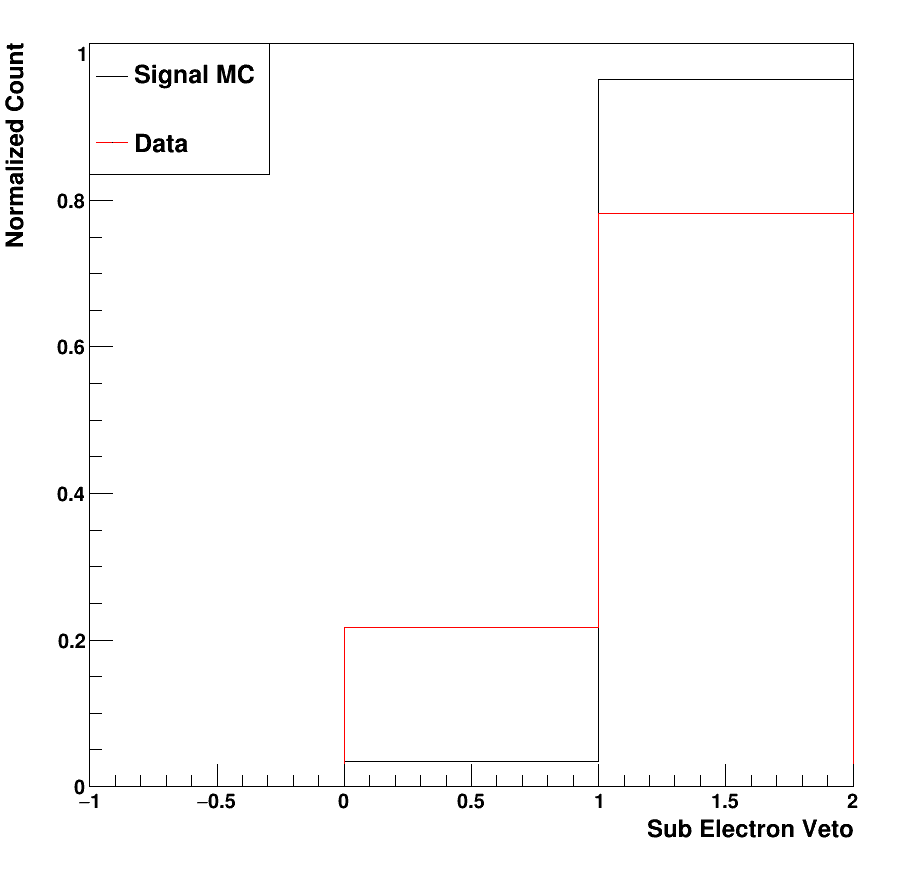
\includegraphics[width=\linewidth]{./Figures/Offline Selection Plots/DiHiggs/0715_DiphotonBDT_TrainingPlots/subElectronVeto.png}
		\caption{Sub Electron Veto}
		\label{DiphoVars:DiHiggs:subElectronVeto}
	\end{subfigure}
	\caption{The lead and sublead electron veto The signal MC is in black, whereas the data events are in red.}
	\label{fig:DiHiggs:DiphoVars6}
\end{figure}

Finally, the electron veto values look very similar to those of the single Higgs data and MC. Shown in figure \ref{fig:DiHiggs:DiphoVars6}, it is still the case that the signal MC has both photons passing the veto in \textgreater 95\% of cases. Again, this will prove a very useful discrimination variable.

For this final BDT, the same steps of hyperparameter optimization and training were followed. It was found that, for the diHiggs diphoton BDT, the same hyperparameters could be used as for the single Higgs version of the same BDT. 

\chapter{Evaluation of the MVA-HLT and Complementary Offline Selection} \label{chapter:Results}

\section{Measurement of Trigger Rate and Timing} \label{sec:TriggerRate}
[I need an academic source for this section -- ask Marco?]
As discussed in chapter \ref{chapter:HLT}, the first main consideration for any HLT is the trigger rate, usually measured in Hz. There are two main corresponding numbers: the total rate measures the total number of events being accepted by the trigger, whereas the pure rate measures the number of events being accepted by a trigger that would not be accepted by any other trigger. In addition to the rate of accepted data, the overall timing of the trigger is of vital importance. Given the speed with which events are read out from the L1 triggers, every milisecond of computation time is a vital resource to be spent sparingly. 

Standardized tools to evaluate the timing and rate of the HLT paths exist (REF?). Firstly, for the timing, special L1 skim files exist which are earmarked for trigger rate measurement. Existing software can be run that measures both the total and pure rates of any selection of triggers. This software returned a total rate of 61.53 Hz of events for the sHLT. The MVA-HLT, on the other hand, yielded a total rate of 29.43 Hz. This measurement is quite in line with the preliminary results shown in section \ref{sec:onlineEfficiencies}. This 52.2\% relative reduction in trigger rate will be further examined in section \ref{sec:OfflineHLTSingleH}. Additionally, the pure rate of the MVA-HLT was measured to be 8.03 Hz. This represents a relatively small addition of events in the overall scale of the trigger rate, and is therefore acceptable. In fact, some degree of pure rate is to be expected given the lowered $p_T$ thresholds for this trigger.

As with the trigger rate, standardized tools exist to measure the HLT path timing (REF?). This measurement runs over a small number of data events and measures the path timing for the whole trigger menu simultaneously. The sHLT, in this framework, takes approximately 15.8ms of processing time. In comparison, the MVA-HLT takes about 15.5ms. While this software doesn't provide uncertainties on these measurements, repeated runs show that the resulting timing values may vary by a few tenths of a milisecond. So, then, it appears that these path timings are relatively consistent with each other. Overall, the important fact is that the MVA-HLT does not take any unduly large amount of processing time; given the application of the BDT within the path, this was a major consideration during the development of the trigger. Additionally, similar software can run to measure the total event throughput per second of the entire HLT menu. This measurement can be run with and without the presence of the MVA-HLT. Running the full menu yields a throughput of $526.2 \pm 2.7$ events/second. Running with the MVA-HLT added in yields a throughput of $524.8 \pm 3.1$ events/second. These measurements are clearly within uncertainties of each other, and it can therefore be concluded that the presence of the MVA-HLT does not measurably impact the overall timing of the trigger menu. 

\section{Evaluation of MVA-HLT Eficiency on Selected Signal Samples}
Once it has been verified that the trigger rate is within the limits posed by the collaboration, the next major task is ensuring that the signal efficiency for the MVA-HLT is a noticable improvement over the standard HLT.  Since the reconstruction, calibrations, and corrections are different at the NanoAOD level, the measurements made at the RAW level in section \ref{sec:cutChoices} must be verified on independent analysis-level (NanoAOD) samples. HiggsDNA was used to produce these samples and plots, which is described in more detail in \ref{sec:HiggsDNA}. One major point of note is that here the "All Events" curve shown must be carefully defined. For these MVA-HLT plots, there will be no additional preselection. Only minimal kinematic cuts of $p_T > 14.25$, $\lvert \eta_{SC} \rvert < 2.5$, and $100 < M_{\gamma \gamma} < 180$ are applied. Additionally, both the signal and data are required to pass one or both of the triggers of interest. So, every event replicated below will pass either the sHLT, MVA-HLT, or both. 

As in section \ref{sec:cutChoices}, plots can be made of selected input variables and the resulting accepted distributions can be compared for the MVA-HLT versus the standard diphoton HLT. For these susequent plots, the acceptance of MVA-HLT will be shown in dark blue, while the acceptance of the standard HLT will be shown in dark blue. Additionally, the light blue curve will show events that pass the MVA-HLT but fail the standard HLT. Therefore, the light blue curve will our signal gain directly. 

In order to assess these results in terms of real physics yeilds, the counts of signal and data must be luminosity-normalized. The EGamma dataset for the 2024I run consists of a total of 11.56 $fb^{-1}$ of integrated luminosity. In contrast, monte carlo signal samples are produced with a specific number of events in mind. Then, an "equivalent luminosity" is calculated, essentially measuring how much real integrated luminosity would be required to capture the generated number of events. Additionally, each MC has an associated cross-section ($\sigma$) given in pb. When combining this with the event-by-event weights calculated at the generator, the number of expected events can be constructed as given in equation \ref{eqn:ExpectedCount}. The ratio at the end of the equation, ($\mathcal{L}_{Target}/\mathcal{L}_{Equiv.}$) is added so that the MC counts are scaled to the same luminosity as the selected data.
\begin{equation}\label{eqn:ExpectedCount}
    Expected Count = Event Weight * \sigma (pb) * \mathcal{L}_{Equiv.} (fb^{-1}) * 1000 * \left(\frac{\mathcal{L}_{Target} (fb^{-1})}{\mathcal{L}_{Equiv.} (fb^{-1})}\right)
\end{equation}

\subsection{$H \rightarrow \gamma \gamma$ MVA-HLT Acceptance} \label{sec:OfflineHLTSingleH}
Beginning with the $M_{\gamma \gamma}$ distribution (fig. \ref{fig:SingleH:HLTAcceptance:Mgg}), it can be seen that the MVA-HLT (blue) has considerably improved signal MC acceptance compared to the standard HLT. In fact, there is a 9.7\% relative signal efficiency gain (97.32\% vs 88.68\%) when considering both the barrel and endcap events together. This is a bit lower than the 13.6\% signal gain seen at the RAW trigger level (93.86\% vs 82.64\%). This is partly due to the improvement in overall signal efficiency for the standard HLT at the NanoAOD level. Because the NanoAOD reconnstruction is imrpoved relative to that at the trigger RAW level, it is expected that the total signal efficiency at this level will be improved. Overall, however, it can be seen that the $H \rightarrow \gamma \gamma$ signal eficiency is very high for the MVA-HLT, as desired.

Another major advantage of the MVA-HLT is the reduction in data rate. As demonstrated in section \ref{sec:TriggerRate}, the MVA-HLT has approximately half the trigger rate of the standard trigger. This is approximately confirmed by data distribution shown in \ref{SingleHBkg:HLTAcceptance:Mgg}. For all $\eta_{SC}$, the total data acceptance is 22.41\% compared to thr 42.62\% of the standard HLT. The light blue curve, additionally, can be used as a proxy for seeing the pure rate measured in section \ref{sec:TriggerRate}; about 13.4\% of the data passes the MVA-HLT but fails the standard HLT. 

\begin{figure}[H]
	\begin{subfigure}{0.50\linewidth}
		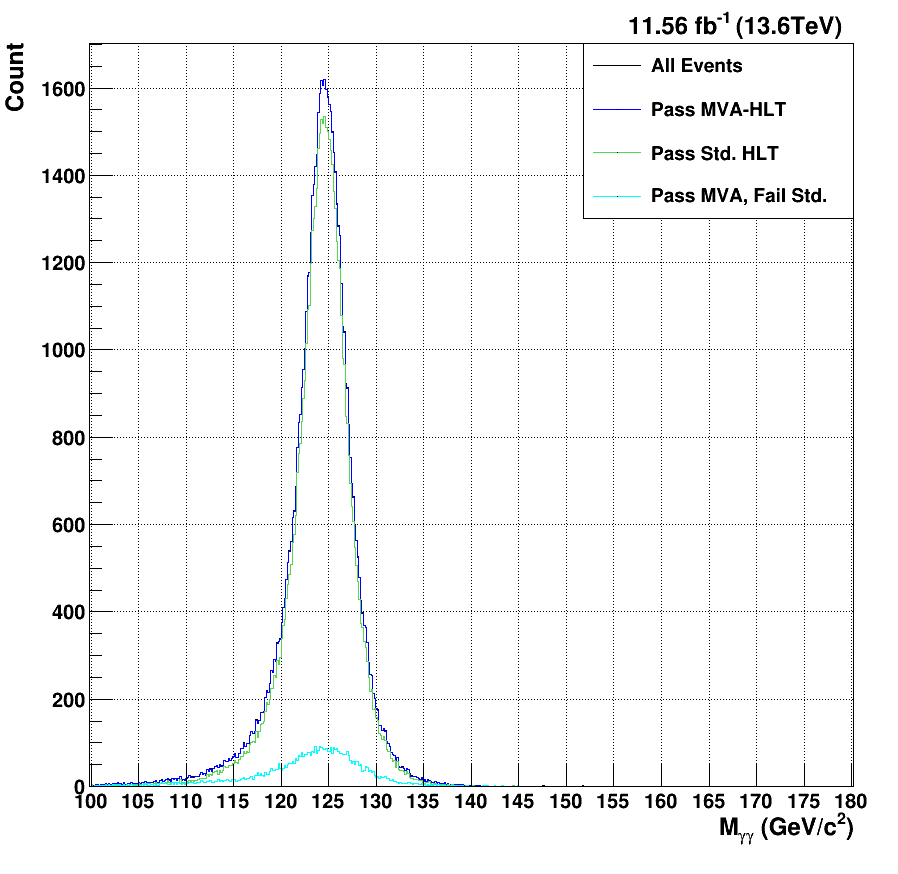
\includegraphics[width=\linewidth]{./Figures/Offline Selection Plots/0710_HLTOfflineAcceptance_WithPassFail_SingleSquarePlots/hggMass_All_Sig.png}
		\caption{Signal MC $M_{\gamma \gamma}$}
		\label{SingleHSig:HLTAcceptance:Mgg}
	\end{subfigure}\hfill
	\begin{subfigure}{0.50\linewidth}
		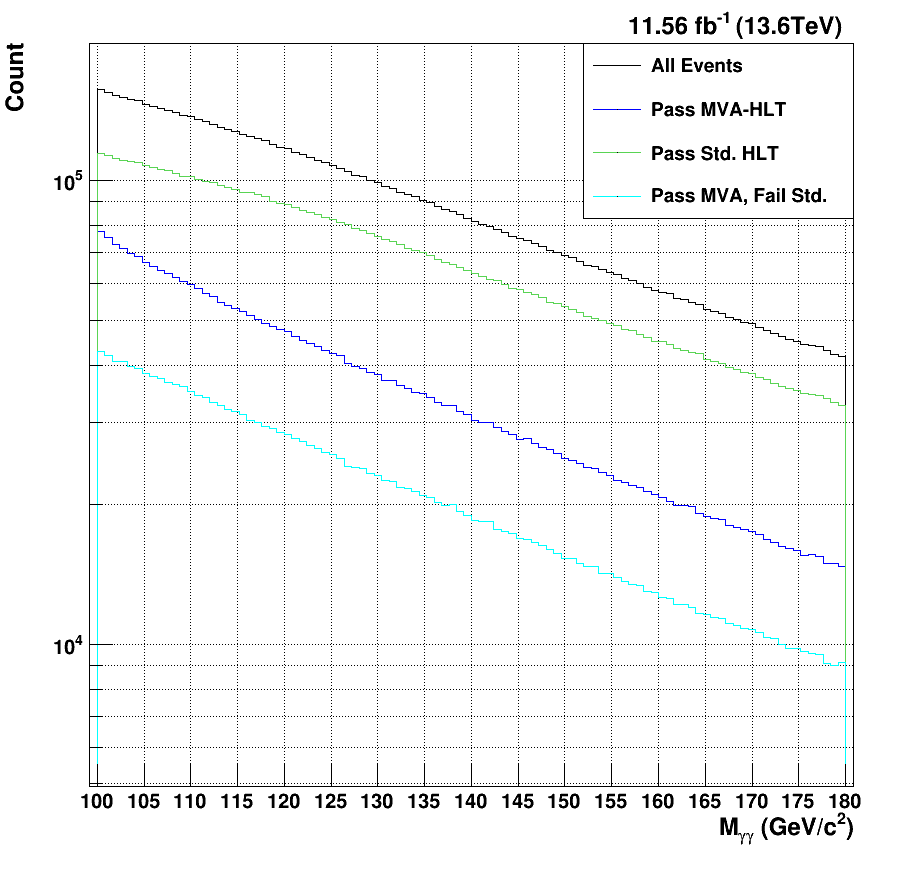
\includegraphics[width=\linewidth]{./Figures/Offline Selection Plots/0710_HLTOfflineAcceptance_WithPassFail_SingleSquarePlots/hggMass_All_Bkg.png}
		\caption{Data $M_{\gamma \gamma}$}
		\label{SingleHBkg:HLTAcceptance:Mgg}
	\end{subfigure}
	\caption{$H \rightarrow \gamma \gamma$ acceptance of the MVA-HLT (dark blue) vs. the current standard diphoton HLT (green) for $M_{\gamma \gamma}$. Events that pass the MVA-HLT but fail the standard HLT can be seen in light blue.}
	\label{fig:SingleH:HLTAcceptance:Mgg}
\end{figure}

Next, the acceptance in the trigger in $\eta_{SC}$ \ref{fig:SingleH:HLTAcceptance:Eta} can be considered. The MVA-HLT has relatively consistent acceptance in $\eta_{SC}$, whereas the standard trigger shows holes in the acceptance in the lowest-$\eta$ regions of the endcap. Investigations have shown that the $R_9$ cuts of the standard trigger are responsible for this inefficiency. As seen in the light blue curve, the MVA-HLT is able to close this gap and provide more consistent kinematic coverage. Otherwise, the gain relative to the standard MVA-HLT is relatively flat throughout the barrel and the rest of the endcap. These features shown that the kinematic coverage is improved relative to that of the standard HLT.

The acceptance of the data, shown in figure \ref{SingleHBkg:HLTAcceptance:Eta}, shows a few relevant features. Whereas the standard HLT accepts more data in the center of the barrel and cuts out more of the barrel above $\lvert \eta_{SC} \rvert > 1.0$. The MVA-HLT, on the other hand, exhibits the opposite features. In the data, the standard HLT closely matches the shape of the full distribution in black, including considerable acceptance in the high-$\eta$ horns. The MVA-HLT is relatively flat throughout the enecap, though it does also accept a small amount more data in the high-$\eta$ horns.

\begin{figure}[H]
	\begin{subfigure}{0.50\linewidth}
		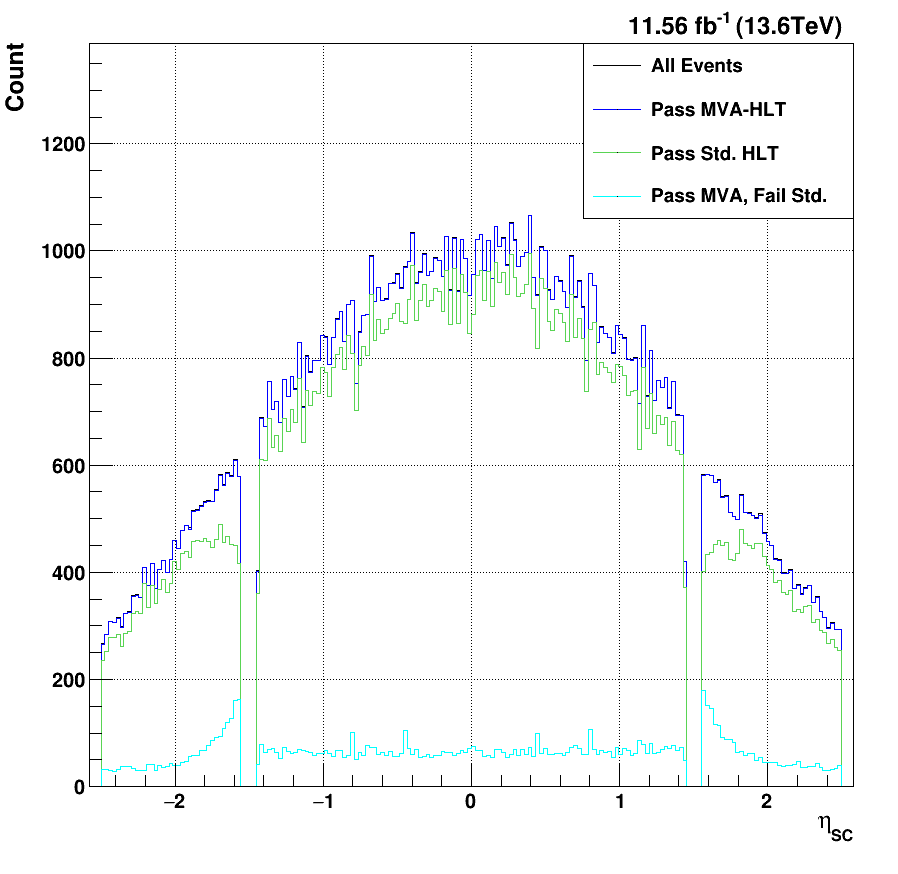
\includegraphics[width=\linewidth]{./Figures/Offline Selection Plots/0710_HLTOfflineAcceptance_WithPassFail_SingleSquarePlots/scEta_All_Sig.png}
		\caption{Signal MC $\eta_{SC}$}
		\label{SingleHSig:HLTAcceptance:Eta}
	\end{subfigure}\hfill
	\begin{subfigure}{0.50\linewidth}
		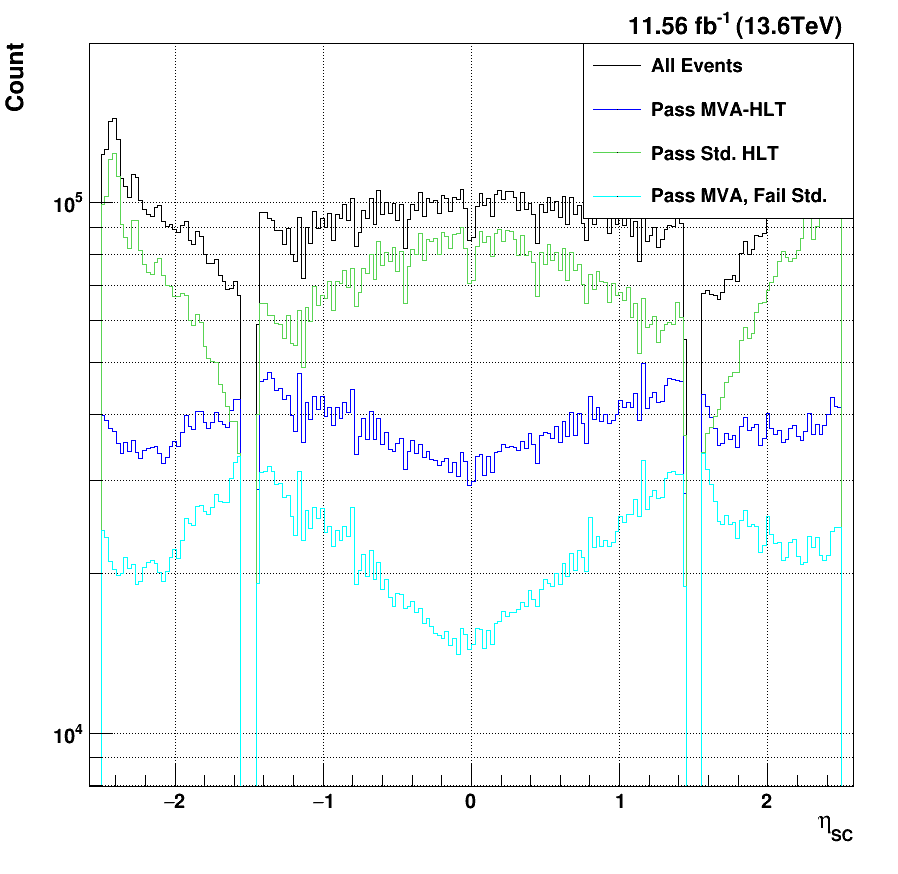
\includegraphics[width=\linewidth]{./Figures/Offline Selection Plots/0710_HLTOfflineAcceptance_WithPassFail_SingleSquarePlots/scEta_All_Bkg.png}
		\caption{Data $\eta_{SC}$}
		\label{SingleHBkg:HLTAcceptance:Eta}
	\end{subfigure}
	\caption{$H \rightarrow \gamma \gamma$ acceptance of the MVA-HLT (dark blue) vs. the current standard diphoton HLT (green) for $\eta_{SC}$. Both the lead and sublead photons are plotted together. Events that pass the MVA-HLT but fail the standard HLT can be seen in light blue.}
	\label{fig:SingleH:HLTAcceptance:Eta}
\end{figure}

Next, the photon candidate $p_T/M_{\gamma \gamma}$ can be examined. Given the lower $p_T$ thresholds of the MVA-HLT, it is expected that there will be some enhancement in acceptance for low-$p_T$ candidates. For the sHLT, the signal MC in figure \ref{SingleHSig:HLTAcceptance:Ptm} goes to 0 around $p_T/M_{\gamma \gamma} = 0.15$, which corresponds to the sublead $p_T > 25$ cut. This leads to an enhancement in the gain below this value, as the MVA-HLT keeps consistent kinematic coverage down to the lowerst values plotted. Of course, these low-$p_T/M_{\gamma \gamma}$ sublead photons correspond to a higher-$p_T/M_{\gamma \gamma}$ lead photon, which is usually not cut out by the sHLT. Since the HLT is a per-event decision, both of these photons will be cut out by the sHLT. So, gains across the whole $p_T/M_{\gamma \gamma}$ range can be seen for the MVA-HLT. For the background, it can be seen that the sHLT begins to fall off at lower values. The MVA-HLT achieves considerably lower data acceptance without explicity cutting out any region of the $p_T/M_{\gamma \gamma}$ distribution. 
\begin{figure}[H]
	\begin{subfigure}{0.50\linewidth}
		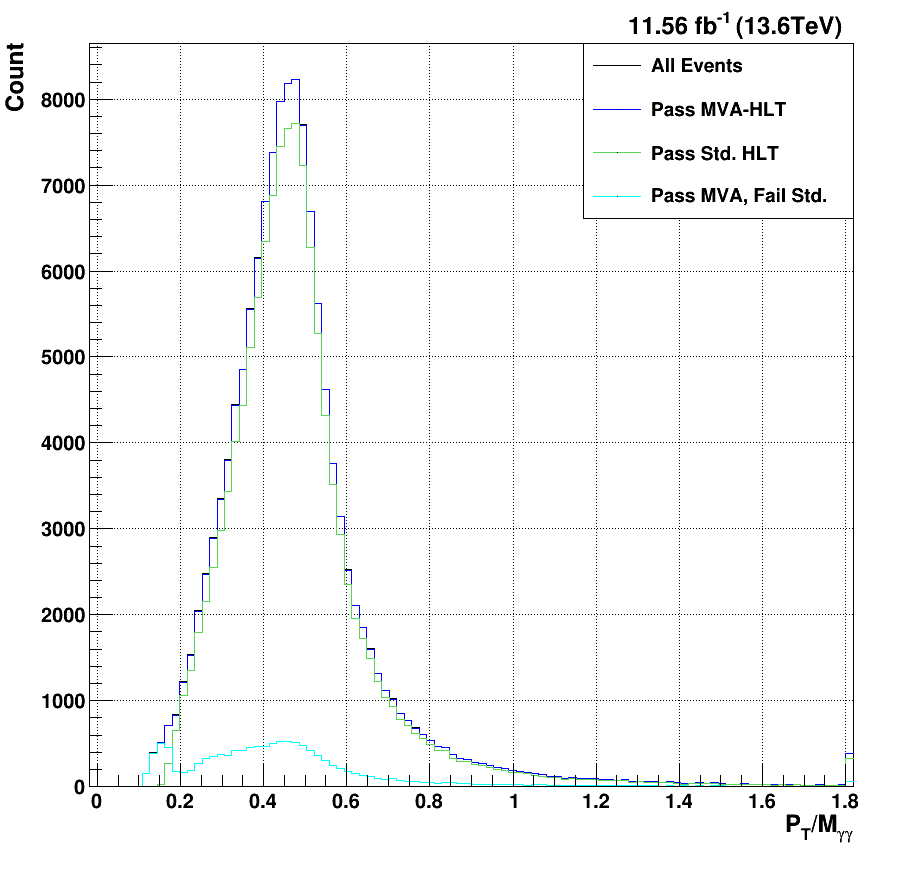
\includegraphics[width=\linewidth]{./Figures/Offline Selection Plots/0710_HLTOfflineAcceptance_WithPassFail_SingleSquarePlots/ptOvrM_All_Sig.png}
		\caption{Signal MC Diphoton $p_{T}$}
		\label{SingleHSig:HLTAcceptance:Ptm}
	\end{subfigure}\hfill
	\begin{subfigure}{0.50\linewidth}
		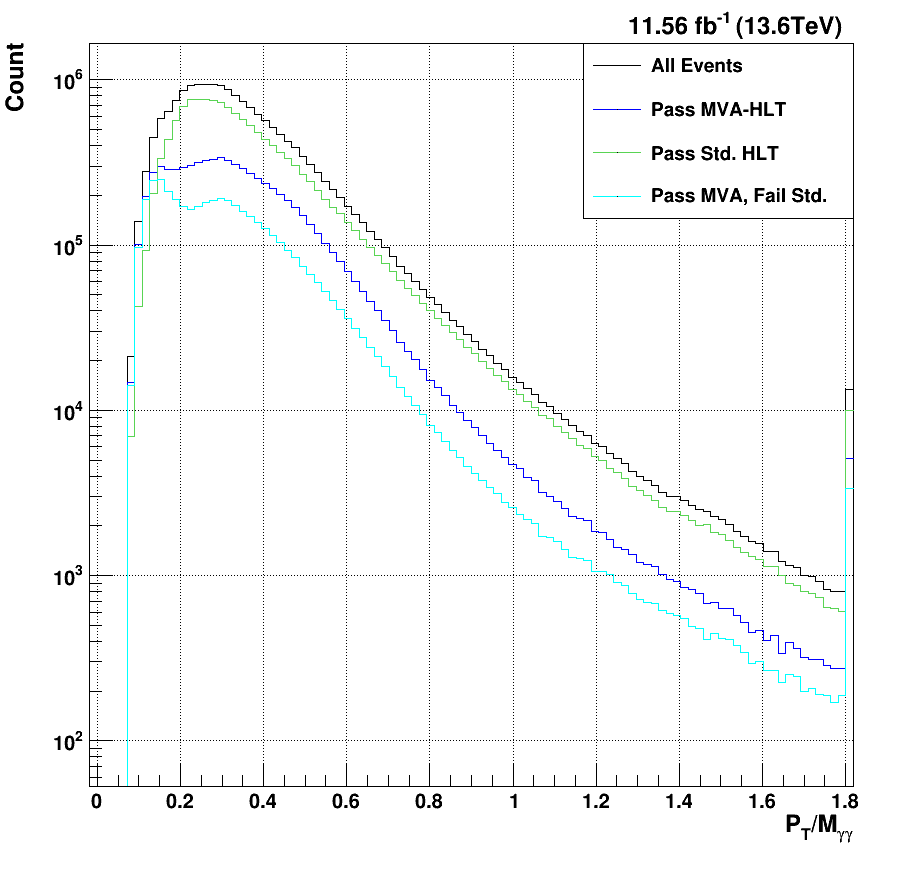
\includegraphics[width=\linewidth]{./Figures/Offline Selection Plots/0710_HLTOfflineAcceptance_WithPassFail_SingleSquarePlots/ptOvrM_All_Bkg.png}
		\caption{Data Diphoton $p_{T}$}
		\label{SingleHBkg:HLTAcceptance:Ptm}
	\end{subfigure}
	\caption{$H \rightarrow \gamma \gamma$ acceptance of the MVA-HLT (dark blue) vs. the current standard diphoton HLT (green) for $p_{T}$. Both the lead and sublead photons are plotted together. Events that pass the MVA-HLT but fail the standard HLT can be seen in light blue.}
	\label{fig:SingleH:HLTAcceptance:Ptm}
\end{figure}

Finally, the results of the signal MC efficiency and the data acceptance are tabulated in table \ref{tab:offlineHLTEffs}. The different $\eta_{SC}$ configurations are separated here -- B-B and E-E events correspond to both photons being located in the barrel and endcap, respectively, while the B-E events have one photon in the barrel and the other in the endcap. Immediately, it can be seen that the MVA-HLT has relatively constant signal acceptance for each region, varrying by a total of 3.45\% between the B-E events (95.2\%) and the B-B events (93.39\%). Meanhile, the standard HLT has considerably reduced signal efficiency in the B-E. This allows the MVA-HLT to have a relative efficency gain of 17.1\% in this region. This is another way in which the kinematic coverage of the MVA-HLT is greatly improved relative to the standard HLT. 

\begin{table}[h]
    \centering
    \caption{$H \rightarrow \gamma \gamma$ signal efficiencies and background acceptances for both triggers, broken down by the location of each photon candidate in $\eta_{sc}$.}
	\label{tab:offlineHLTEffs}
    \begin{subtable}{.49\textwidth}
        \centering
        \caption{Signal Efficiencies}
        \begin{tabular}{|c|c|c|}
            \hline
            \textbf{Region} & \textbf{MVA-HLT(\%)} & \textbf{Std. HLT(\%)}\\
			\Xhline{2pt}
            B-B & 98.65 & 93.39 \\ \hline
            B-E & 95.20 & 81.27\\ \hline
            E-E & 96.70 & 86.24\\ \hline
            All & 97.32 & 88.68 \\ \hline
        \end{tabular}
    \end{subtable}
    \hfill
	\begin{subtable}{.49\textwidth}
        \centering
        \caption{Data Acceptances}
        \begin{tabular}{|c|c|c|}
            \hline
            \textbf{Region} & \textbf{MVA-HLT(\%)} & \textbf{Std. HLT(\%)}\\
			\Xhline{2pt}
            B-B & 21.07 & 37.27 \\ \hline
            B-E & 23.11 & 46.57 \\ \hline
            E-E & 22.26 & 32.32 \\ \hline
            All & 22.41 & 42.62 \\ \hline
        \end{tabular}
    \end{subtable}
\end{table}

Overall, it can be seen that the MVA-HLT achieves the desired result at the NanoAOD analysis level. The signal efficiency is about 9.7\% higher for the $H \rightarrow \gamma \gamma$ signal MC relative to the standard HLT. The overall efficiency sits at 97.3\%, which allows virtually all of the signal MC to be considered for subsequent analyses. In addition, no holes in kinematic coverage can be seen, meaning that the MVA-HLT is able to more-completely cover the full range of possible physics that can be gleaned from $H \rightarrow \gamma \gamma$ processes.

\subsection{$HH \rightarrow b \bar{b} \gamma \gamma$ MVA-HLT Acceptance} \label{sec:OfflineHLTDiHiggs}

Where the MVA-HLT can sine best, however, is for more rare processes like the $HH \rightarrow b \bar{b} \gamma \gamma$. As with the single Higgs results, plots can be made comparing the signal efficiency and data acceptance for the sHLT versus the MVA-HLT. These distributions are shown in figures \ref{fig:DiHiggs:HLTAcceptance:Mgg}-\ref{fig:DiHiggs:HLTAcceptance:Ptm}. Given that the cross section of the DiHiggs is much lower than that of the single Higgs (as described in section \ref{sec:Higgs}), the equivalent counts for this signal MC are lower.

Similarly to the MVA-HLT results for the $H \rightarrow \gamma \gamma$ signal MC, very high signal efficiency is immediately seen for $HH \rightarrow b \bar{b} \gamma \gamma$. In figure \ref{fig:DiHiggs:HLTAcceptance:Mgg}, it can be seen that the signal acceptance has near-perfect kinematic coverage in $M_{\gamma \gamma}$ and achieves a total efficiency of 98.45\%. Compared to the sHLT (88.45\%), this is an 11.3\% relative gain.  This is, in fact, slightly higher than the 97.32\% achieved for the single Higgs. Since the MVA-HLT is largely aimed at improving the signal efficiency for rarer processes, this is a welcome result. The data acceptance is lower than that for the single Higgs, but the ratio between the sHLT and the MVA-HLT is approximately constant -- while the sHLT accepts 33.2\% of the data, the MVA-HLT accepts 16.86\%. There is no particular $M_{\gamma \gamma}$ dependence to the acceptance of either HLT for the signal or background.

\begin{figure}[H]
	\begin{subfigure}{0.50\linewidth}
		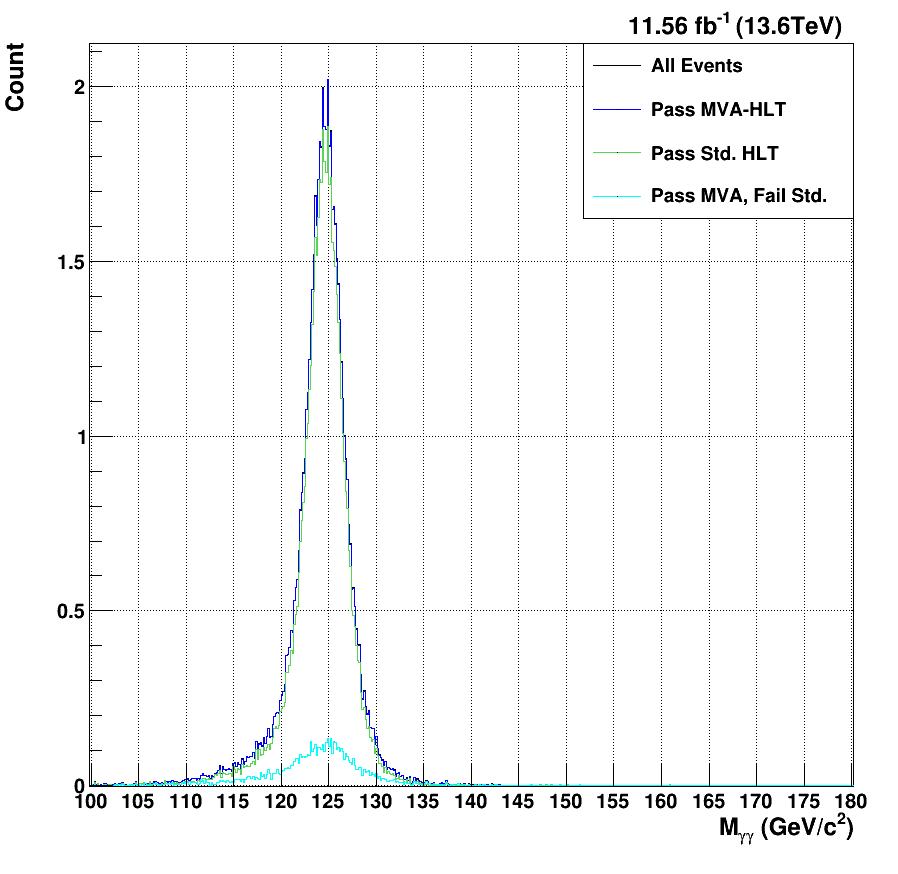
\includegraphics[width=\linewidth]{./Figures/Offline Selection Plots/DiHiggs/0715_HLTOfflineAcceptance_WithPassFail_SingleSquarePlots/hggMass_All_Sig.png}
		\caption{Signal MC $M_{\gamma \gamma}$}
		\label{DiHiggsSig:HLTAcceptance:Mgg}
	\end{subfigure}\hfill
	\begin{subfigure}{0.50\linewidth}
		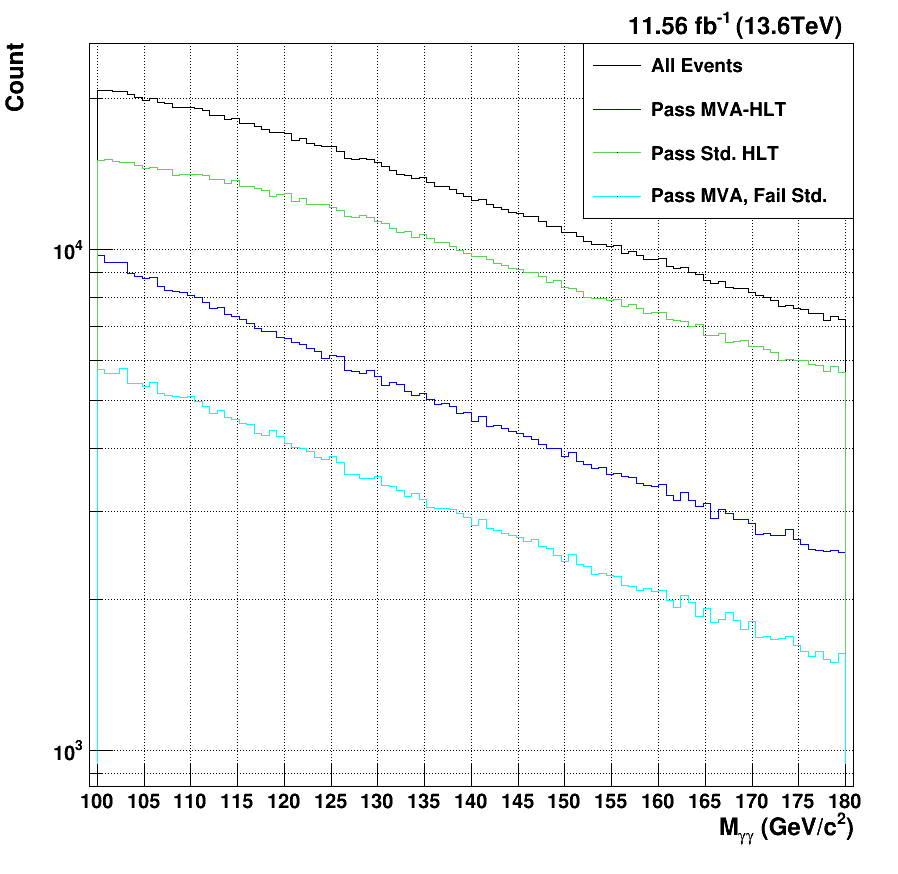
\includegraphics[width=\linewidth]{./Figures/Offline Selection Plots/DiHiggs/0715_HLTOfflineAcceptance_WithPassFail_SingleSquarePlots/hggMass_All_Bkg.png}
		\caption{Data $M_{\gamma \gamma}$}
		\label{DiHiggsBkg:HLTAcceptance:Mgg}
	\end{subfigure}
	\caption{$HH \rightarrow b \bar{b} \gamma \gamma$ acceptance of the MVA-HLT (dark blue) vs. the current standard diphoton HLT (green) for $M_{\gamma \gamma}$. Events that pass the MVA-HLT but fail the standard HLT can be seen in light blue.}
	\label{fig:DiHiggs:HLTAcceptance:Mgg}
\end{figure}

Upon examining the $\eta_{SC}$ distributions, the kinematic differences between the single Higgs and diHiggs are again borne out; the $HH \rightarrow b \bar{b} \gamma \gamma$ signal MC tends to have far fewer events in the endcap and is quite central near 0 for the barrel. The same gains in signal efficiency around the low-$\eta$ endcap can be seen, though they are smaller for the DiHiggs. The shape of the background acceptance is essentially unchanged, though the dip at $\eta = 0$ is perhaps marginally larger. Again, this reaffirms the fact that the kinematic coverage in $\eta_{SC}$ is improved for the signal MC relative to the MVA-HLT.

\begin{figure}[H]
	\begin{subfigure}{0.50\linewidth}
		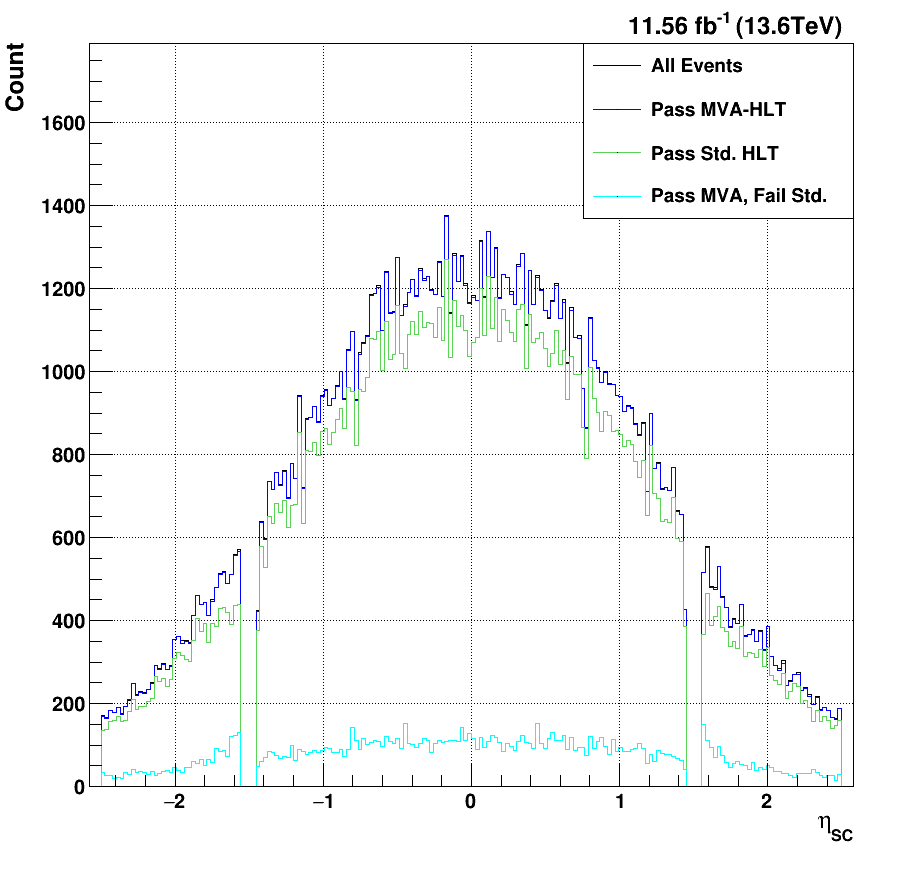
\includegraphics[width=\linewidth]{./Figures/Offline Selection Plots/DiHiggs/0715_HLTOfflineAcceptance_WithPassFail_SingleSquarePlots/scEta_All_Sig.png}
		\caption{Signal MC $\eta_{SC}$}
		\label{DiHiggsSig:HLTAcceptance:Eta}
	\end{subfigure}\hfill
	\begin{subfigure}{0.50\linewidth}
		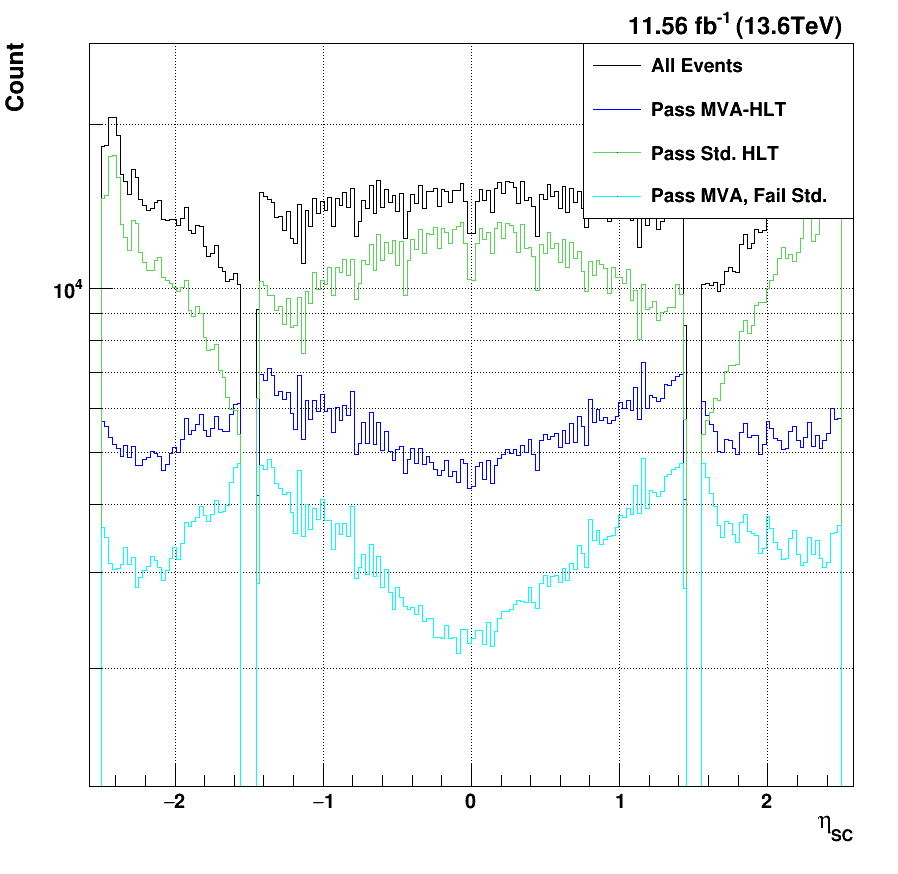
\includegraphics[width=\linewidth]{./Figures/Offline Selection Plots/DiHiggs/0715_HLTOfflineAcceptance_WithPassFail_SingleSquarePlots/scEta_All_Bkg.png}
		\caption{Data $\eta_{SC}$}
		\label{DiHiggsBkg:HLTAcceptance:Eta}
	\end{subfigure}
	\caption{$HH \rightarrow b \bar{b} \gamma \gamma$ acceptance of the MVA-HLT (dark blue) vs. the current standard diphoton HLT (green) for $\eta_{SC}$. Events that pass the MVA-HLT but fail the standard HLT can be seen in light blue.}
	\label{fig:DiHiggs:HLTAcceptance:Eta}
\end{figure}

As seen in figure \ref{DiHiggsSig:HLTAcceptance:Eta}, the diHiggs signal MC shows some clear kinematic differences compared to the single Higgs MC. Whereas the single Higgs drops off much faster in $p_T/M_{\gamma \gamma}$, the diHiggs distribution is much broader and extends to higher values. In fact, the overflow bin in the distribution has a very high population, showing that the distribution continues on for quite some time past the bounds of the graph shown. Like the single Higgs, however, the sHLT cuts out the low-$p_T/M_{\gamma \gamma}$ values. The MVA-HLT keeps virtually all of these photons, meaning that there is considerable gain in signal efficiency in this region. The behavior of the data is much the same as that of the single Higgs. 

\begin{figure}[H]
	\begin{subfigure}{0.50\linewidth}
		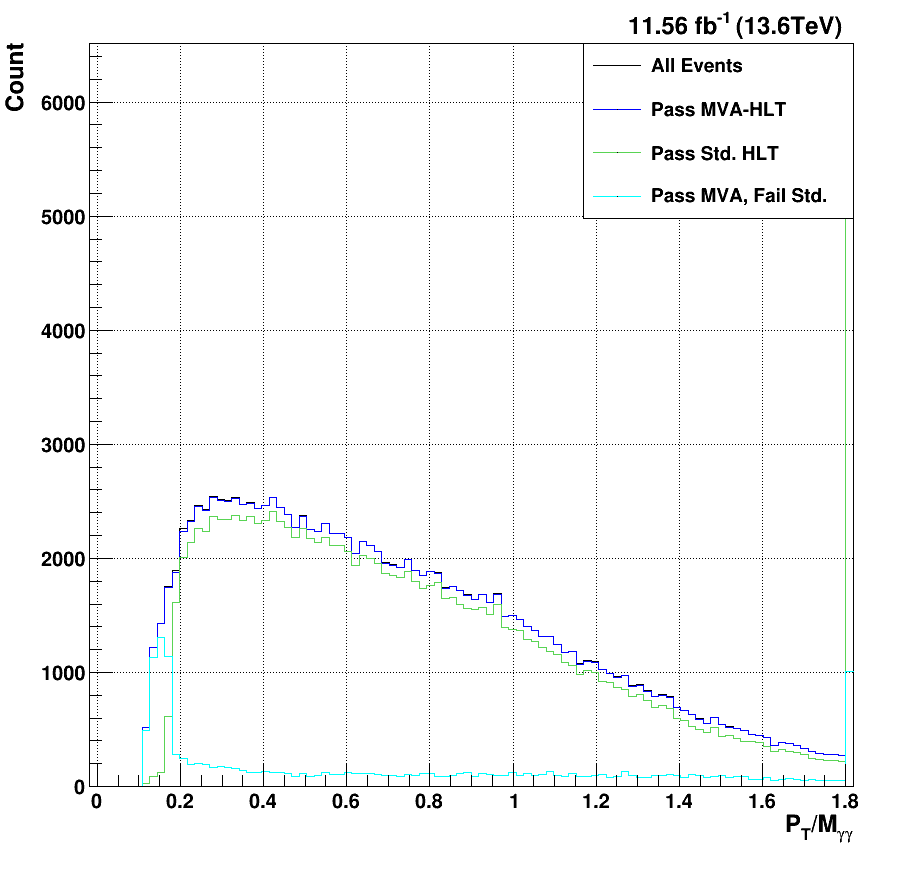
\includegraphics[width=\linewidth]{./Figures/Offline Selection Plots/DiHiggs/0715_HLTOfflineAcceptance_WithPassFail_SingleSquarePlots/ptOvrM_All_Sig.png}
		\caption{Signal MC $p_T/M_{\gamma \gamma}$}
		\label{DiHiggsSig:HLTAcceptance:PtM}
	\end{subfigure}\hfill
	\begin{subfigure}{0.50\linewidth}
		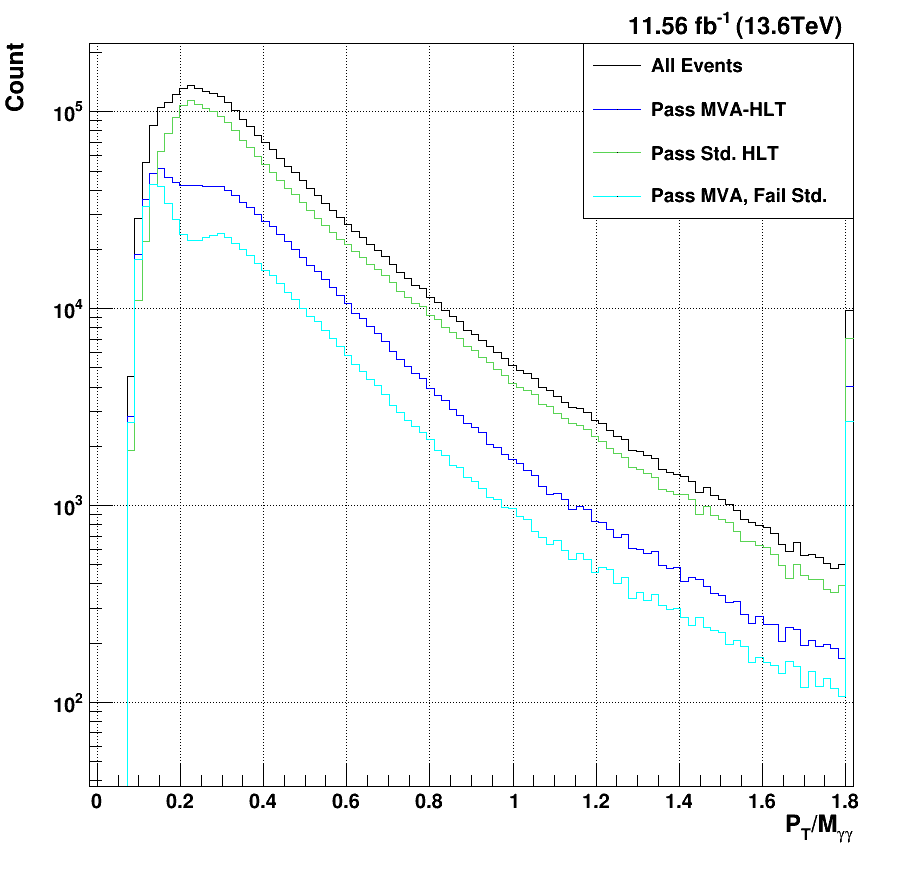
\includegraphics[width=\linewidth]{./Figures/Offline Selection Plots/DiHiggs/0715_HLTOfflineAcceptance_WithPassFail_SingleSquarePlots/ptOvrM_All_Bkg.png}
		\caption{Data $p_T/M_{\gamma \gamma}$}
		\label{DiHiggsBkg:HLTAcceptance:PtM}
	\end{subfigure}
	\caption{$HH \rightarrow b \bar{b} \gamma \gamma$ acceptance of the MVA-HLT (dark blue) vs. the current standard diphoton HLT (green) for $p_T/M_{\gamma \gamma}$. Events that pass the MVA-HLT but fail the standard HLT can be seen in light blue.}
	\label{fig:DiHiggs:HLTAcceptance:Ptm}
\end{figure}

Table \ref{tab:DiHiggs:offlineHLTEffs} shows the total efficiencies for both the $HH \rightarrow b \bar{b} \gamma \gamma$ signal MC and data in the different detector regions. While the signal MC efficiencies for the sHLT are approximately equal to those of the single Higgs, the MVA-HLT achieves marginally high efficiencies in all of the detector regions relative to the single Higgs. The relative gain, as a result, is higher for the diHiggs MVA0-HLT. Meanwhile, the data acceptance of both HLTs is lower than that of the single Higgs, though the relative proportion stays consistent.

\begin{table}[h]
    \centering
    \caption{$HH \rightarrow b \bar{b} \gamma \gamma$ signal efficiencies and background acceptances for both triggers, broken down by the location of each photon candidate in $\eta_{sc}$.}
	\label{tab:DiHiggs:offlineHLTEffs}
    \begin{subtable}{.49\textwidth}
        \centering
        \caption{Signal Efficiencies}
        \begin{tabular}{|c|c|c|}
            \hline
            \textbf{Region} & \textbf{MVA-HLT(\%)} & \textbf{Std. HLT(\%)}\\
			\Xhline{2pt}
            B-B & 98.90 & 91.01 \\ \hline
            B-E & 97.25 & 81.10 \\ \hline
            E-E & 98.26 & 89.18 \\ \hline
            All & 98.45 & 88.45 \\ \hline
        \end{tabular}
    \end{subtable}
    \hfill
	\begin{subtable}{.49\textwidth}
        \centering
        \caption{Data Acceptances}
        \begin{tabular}{|c|c|c|}
            \hline
            \textbf{Region} & \textbf{MVA-HLT(\%)} & \textbf{Std. HLT(\%)}\\
			\Xhline{2pt}
            B-B & 14.73 & 28.12 \\ \hline
            B-E & 18.26 & 37.24 \\ \hline
            E-E & 15.51 & 24.77 \\ \hline
            All & 16.86 & 33.24 \\ \hline
        \end{tabular}
    \end{subtable}
\end{table}

\section{Evaluation of Offline Selection Eficiency with MVA-HLT }
As discussed in chapter \ref{chapter:OfflineSelection}, the offline selection cuts are designed to cover the corresponding HLT cuts. Since the sHLT is based on hard cuts on the $p_T$, showershape, and isolation variables, the offline selection is created using similar principles. The offline selection BDTs developed in chapter \ref{chapter:OfflineSelection} are, on the other hand, designed to cover the MVA-HLT. While the single photon preselection cuts on single Higgs and diHiggs samples were discussed in sections \ref{sec:SingleHSinglePhoCuts} and \ref{sec:DiHiggsSinglePhoCuts}, respectively, the cuts on the corresponding diphoton BDTs were not investigated. The results of these final selections -- applied on top of the corresponding HLT -- will be displayed in this section.

Any chosen offline selection cuts are only given as a point of comparison; the power of a BDT-based approach lies in its ability to be easily tuned for each analysis. As a result, multiple points of comparison will be shown in subsequent plots for both single Higgs and diHiggs samples. Given that this offline selection must compare to that of the standard analysis, this provides a reasonable starting point. So, then, the first diphton BDT cuts will be chosen such that the overall background acceptance of the BDT-based analysis matches that of the standard anylsis. With the same background rate, the improvement in signal efficiency can then be compared as a direct appraisal of the power of the BDT-based analysis. Additionally, selections with one half and twice as much background as the standard analysis will be shown in order to provide additional points of comparison. In sections \ref{sec:OfflineSingleHSelection} and \ref{sec:OfflineDiHiggsSelection} selected variable plots will be displayed for $H \rightarrow \gamma \gamma$ and $HH \rightarrow b \bar{b} \gamma \gamma$, respectively.

For both the single and diHiggs samples, the plots will be shown in much the same way. The same event scaling described in equation \ref{eqn:ExpectedCount} will be used to display the expected counts for the signal MC. The plots will contain six curves total: the black curve will show all reconstructed events selected by the basic selection criteria described before; the dark blue, light blue, and light green will show the standard, tight, and loosest BDT-based selections, respectively; the yellow and orange curves will show the single photon preselection and the overall standard analysis cuts, respctively. 

\subsection{$H \rightarrow \gamma \gamma$ Offline Selection Acceptance}\label{sec:OfflineSingleHSelection}

The $M_{\gamma \gamma}$, shown in figure \ref{fig:SingleH:OfflineAcceptance:Mgg}, contains all of the curves described above. Beginning with the signal in figure \ref{SingleHSig:OfflineAcceptance:Mgg}, the improved signal efficiency of all three BDT-based analyses is immediately manifest. Whereas the standard analysis (SA) cuts only achieve a signal efficiency of 70.53\%, the diphoton BDT cuts that accept the same amount of backround are able to attain a 91.27\% signal efficiency. So, then, the BDT-based selection is not only able to leverage the improved signal performance of the MVA-HLT, but it is able to gain a relative 29.4\% improvement in overall signal efficiency. Even the tight selection, which has half the background acceptance of the SA, reaches a signal efficiency of 83.51\%. The loosest selection, with twice the background of the SA, has a very high signal efficiency of 95.74\%. This selection could be useful for very well-tagged analyses that have some additional criteria that allow the background rate to be brought down considerably without the need for a tight $H \rightarrow \gamma \gamma$ selection.

The shape of the signal mass distribution is, of course, worth investigating. Clearly, with $>90\%$ signal efficiency, the standard BDT-based selection does little to shape the signal MC mass distribution. While the peak of the distribution has very high efficiency, the high- and low-mass tails are also well-preserved. The SA cuts lose considerably signal efficiency in the center of the distribution near $125 GeV/c^2$. There is also a clear reduction in the low-mass tail with the standard selection. As previously discussed, the measure $2\sigma_{Eff.}$ is useful for comparing the overall width of different mass distributions. A lower $2\sigma_{Eff.}$ corresponds to a narrower mass distribution, with often means that the quality of the preserved events in higher. The full distribution measures at $2\sigma_{Eff.} = 5.81 GeV/c^2$. The standard BDT-based selecton cuts out proportionally more of the tail than the center of the distribution, leading to $2\sigma_{Eff.} = 5.58 GeV/c^2$. The SA, on the other hand, cuts out so much of the tails that it achieves $2\sigma_{Eff.} = 5.17 GeV/c^2$. Of course, while the SA cuts are able to reduce the mass width considerably, this comes with a nearly 30\% loss in the signal. While the less rare gluon fusion $H \rightarrow \gamma \gamma$ process faces no major derth of events, this major increase in overall signal efficiency is likely worth an increased mass width for rarer processes.

The background mass distribution in figure \ref{SingleHBkg:OfflineAcceptance:Mgg} also shows a noteworthy difference between the SA and the BDT-Based selections. Firstly, it can be seen that the preselection curve (in yellow) is relatively parallel to the all curve (in black). The SA curve, on the other hand, is considerably steeper; since the only difference between the preselection and SA cuts are the $p_T/M_{\gamma \gamma}$ cuts, it is clear that these cuts are biasing the mass distribution towards lower masses and removing more high-mass background events. This makes sense, as increasing $M_{\gamma \gamma}$ for the same $p_T$ will of course decrease the $p_T/M_{\gamma \gamma}$ and therefore make an event more likely to fail the cuts. While the BDT-based cuts do not show this behavior, they have reversed relationship with $M_{\gamma \gamma}$. Beginning with the loosest cuts in green, the shape differs little from that of the preselection. As the diphoton BDT cuts tighten, however, it is clear that the low-mass region (below $M_{\gamma \gamma} = 125 GeV/c^2$) is cut out considerably. 

\begin{figure}[H]
	\begin{subfigure}{0.50\linewidth}
		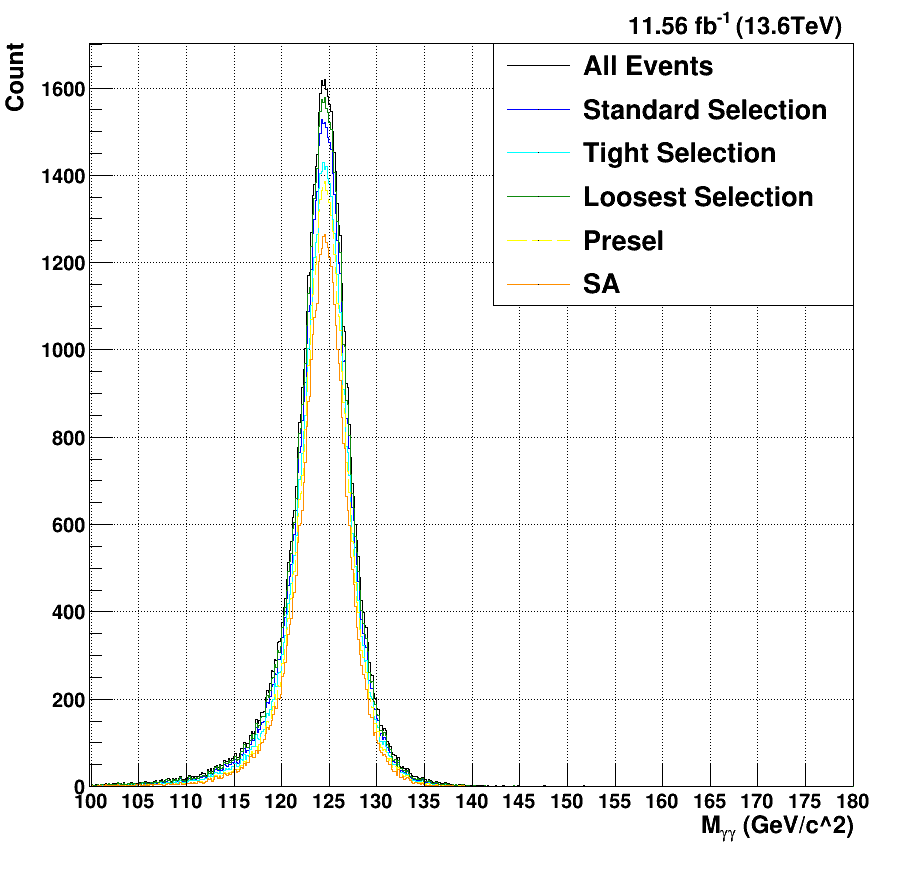
\includegraphics[width=\linewidth]{./Figures/Offline Selection Plots/0710_FullOfflineCuts_SingleSquarePlots/hggMass_All_Sig.png}
		\caption{Signal MC $M_{\gamma \gamma}$}
		\label{SingleHSig:OfflineAcceptance:Mgg}
	\end{subfigure}\hfill
	\begin{subfigure}{0.50\linewidth}
		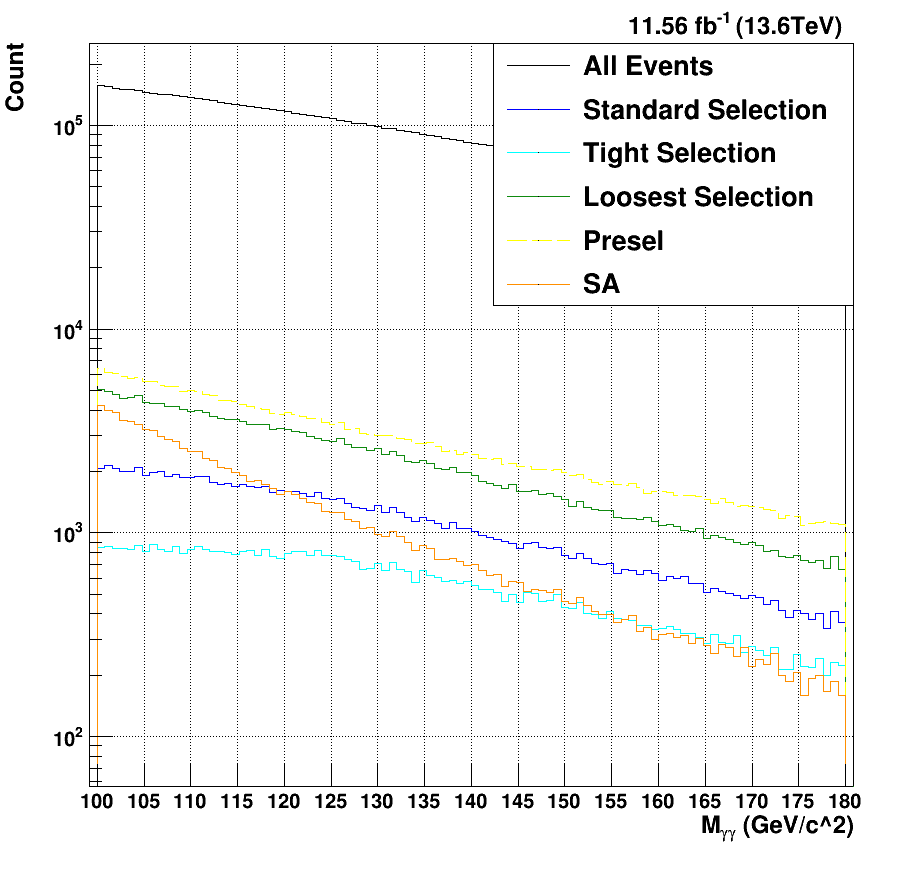
\includegraphics[width=\linewidth]{./Figures/Offline Selection Plots/0710_FullOfflineCuts_SingleSquarePlots/hggMass_All_Bkg.png}
		\caption{Data $M_{\gamma \gamma}$}
		\label{SingleHBkg:OfflineAcceptance:Mgg}
	\end{subfigure}
	\caption{Total offline selection acceptances for $H \rightarrow \gamma \gamma$. Three tightnesses of BDT-based selection cuts are shown in dark blue (standard), light blue (tighter), and light green (looser). The acceptance of the preselection is shown in yellow, while the full standard analysis cuts are shown in orange.}
	\label{fig:SingleH:OfflineAcceptance:Mgg}
\end{figure}

Turning to the signal MC $\eta_{SC}$ in figure \ref{SingleHSig:OfflineAcceptance:ScEta}, clear differences can be seen between the acceptances of the standard analysis cuts and the BDT-based selections. For all three BDT-based selection cuts, the signal efficiency is relatively constant in $\eta_{SC}$. As with the MVA-HLT results shown in the last section, this proves that the BDT-based selection is able to keep great kinematic coverage. The preselection and standard anaylsis, in addition to being much lower throughout the entire $\eta_{SC}$ range, have clear holes in efficiency at the low-$\eta$ regions of the endcap around $\lvert \eta_{SC} \rvert = 1.6$. This mirrors the behavior of the sHLT seen in section \ref{sec:OfflineHLTSingleH}; it has been found that the hard $R_9$ cuts applied by both the sHLT and the preselection considerably decrease the signal efficiency in this region for both standard selections.

There are, additionally, clear differences with the data $\eta_{SC}$ distributions shown in figure \ref{SingleHBkg:OfflineAcceptance:ScEta}. Comparing the standard BDT selection (blue) to the SA cuts (orange), it is immediately clear that the overall acceptance in the barrel detector is relatively equivalent. While the SA cuts seem to cut out slightly more data events at the very ends of the barrel near $\lvert \eta_{SC} \rvert = 1.4$, both selections shown are relatively flat in the barrel. In the endcap, however, some clear distinctions arise. While the SA cuts are relatively flat in the endcap, the BDT-based selections strongly favor the low-$\eta$ regions of the endcap. Since the diphoton BDT for $H \rightarrow \gamma \gamma$ was trained using these signal MC and data distributions, it is expected that the data accepted will approximately follow the shape of the signal MC. Overall, however, this effect is not expected to have a major impact on any analysis.

\begin{figure}[H]
	\begin{subfigure}{0.50\linewidth}
		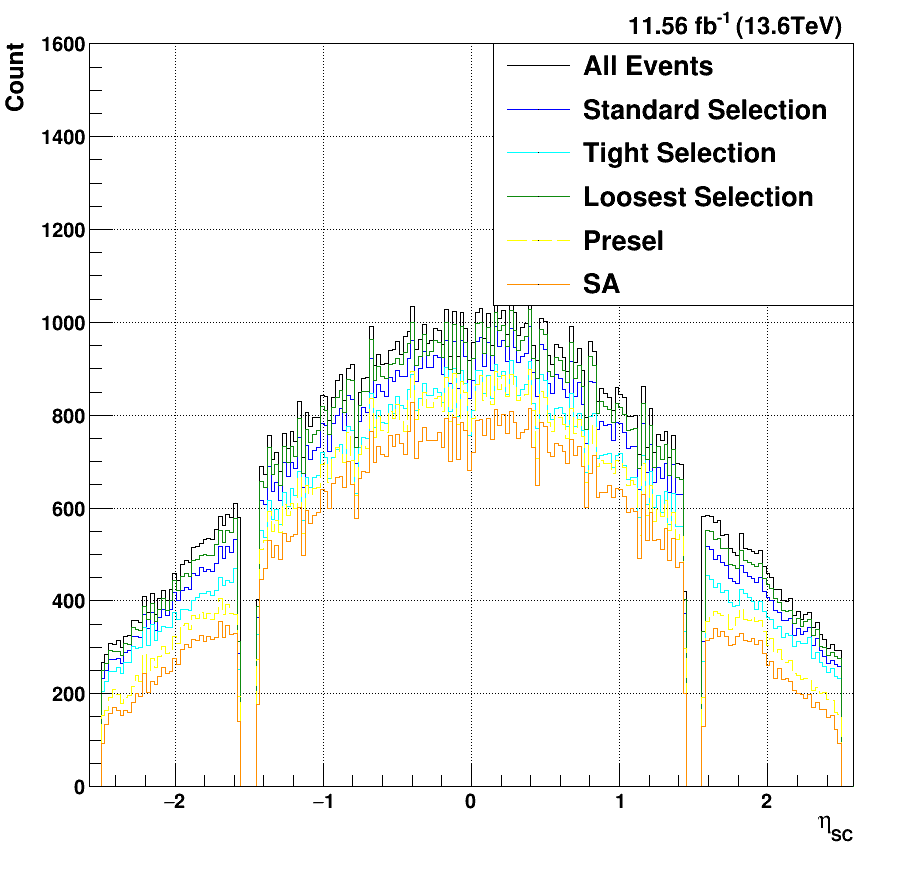
\includegraphics[width=\linewidth]{./Figures/Offline Selection Plots/0710_FullOfflineCuts_SingleSquarePlots/scEta_All_Sig.png}
		\caption{Signal MC $\eta_{SC}$}
		\label{SingleHSig:OfflineAcceptance:ScEta}
	\end{subfigure}\hfill
	\begin{subfigure}{0.50\linewidth}
		\includegraphics[width=\linewidth]{./Figures/Offline Selection Plots/0710_FullOfflineCuts_SingleSquarePlots/scEta_All_Bkg.png}
		\caption{Data $\eta_{SC}$}
		\label{SingleHBkg:OfflineAcceptance:ScEta}
	\end{subfigure}
	\caption{Total offline selection acceptances for $H \rightarrow \gamma \gamma$. Three tightnesses of BDT-based selection cuts are shown in dark blue (standard), light blue (tighter), and light green (looser). The acceptance of the preselection is shown in yellow, while the full standard analysis cuts are shown in orange. Both the lead and sublead photons are plotted together.}
	\label{fig:SingleH:OfflineAcceptance:ScEta}
\end{figure}

The final distribution to consider, as with the HLT results, is the $p_T/M_{\gamma \gamma}$ in figure \ref{fig:SingleH:OfflineAcceptance:PtM}. Given the hard cuts on $p_T/M_{\gamma \gamma}$, the SA cuts show a clear loss of signal efficiency at lower values below about $p_T/M_{\gamma \gamma} < 0.3$. This is one of the major ways this BDT-based analysis is able to increase both the signal efficiency and kinematic coverage relative to the standard selection cuts. By instead accepting signal MC events all the way down to $p_T/M_{\gamma \gamma} = 0.1$, many events that contain a second photon with good $p_T/M_{\gamma \gamma}$ can be preserved for the analysis. Considering the background shown in figure \ref{SingleHBkg:OfflineAcceptance:PtOvrM}, it becomes clear why the $p_T/M_{\gamma \gamma}$ cuts were chosen; many data events fall below the selected thresholds, which makes this selection very effective at reducing the data acceptance. It is clear, however, that the BDT-based approach is still able to reduce the data acceptance to the desired rate while not making stringent requirements on $p_T/M_{\gamma \gamma}$. 

\begin{figure}[H]
	\begin{subfigure}{0.50\linewidth}
		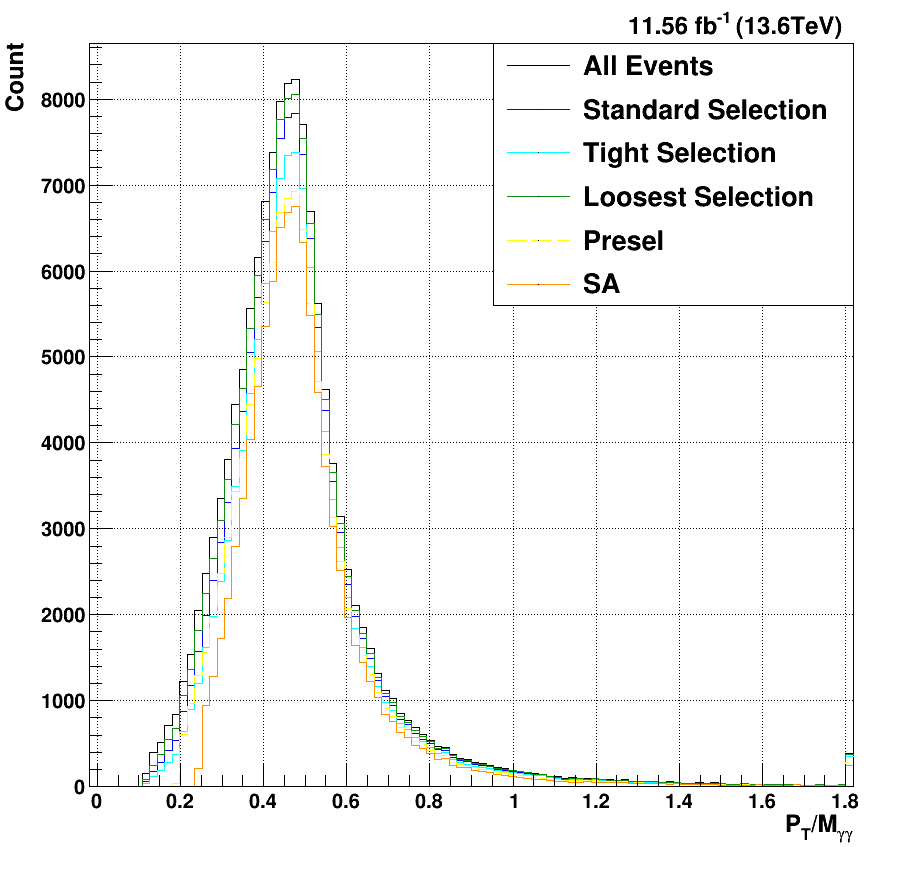
\includegraphics[width=\linewidth]{./Figures/Offline Selection Plots/0710_FullOfflineCuts_SingleSquarePlots/ptOvrM_All_Sig.png}
		\caption{Signal MC $p_T/M_{\gamma\gamma}$}
		\label{SingleHSig:OfflineAcceptance:PtOvrM}
	\end{subfigure}\hfill
	\begin{subfigure}{0.50\linewidth}
		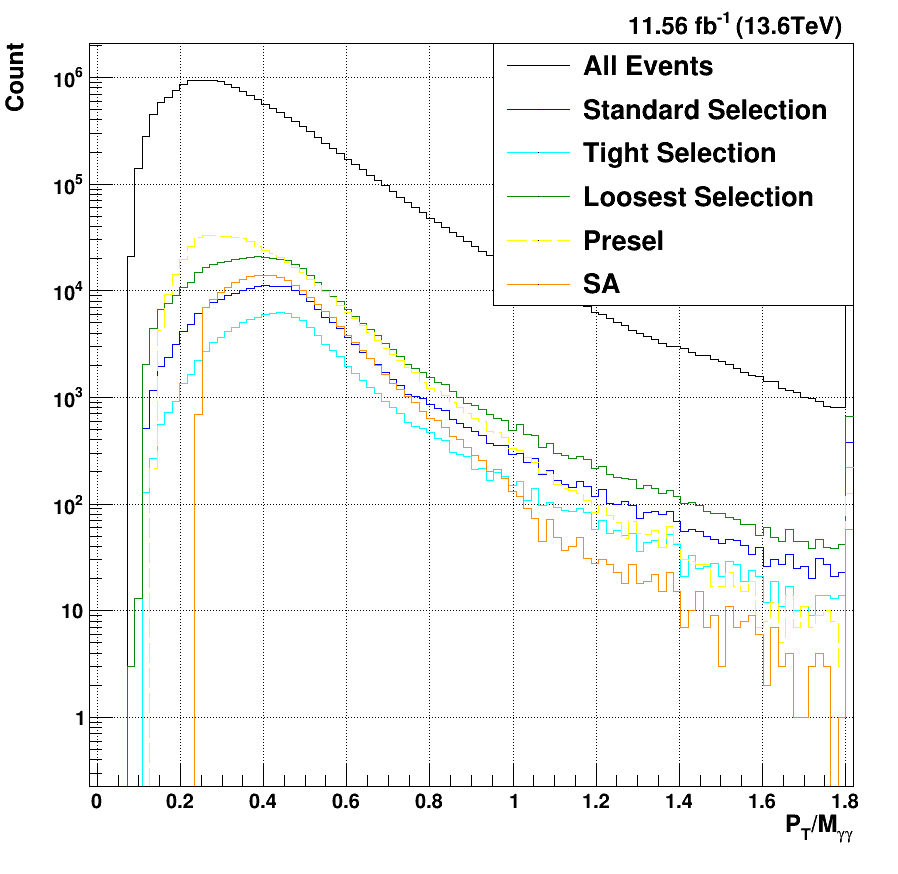
\includegraphics[width=\linewidth]{./Figures/Offline Selection Plots/0710_FullOfflineCuts_SingleSquarePlots/ptOvrM_All_Bkg.png}
		\caption{Data $p_T/M_{\gamma\gamma}$}
		\label{SingleHBkg:OfflineAcceptance:PtOvrM}
	\end{subfigure}
	\caption{Total offline selection acceptances for $H \rightarrow \gamma \gamma$. Three tightnesses of BDT-based selection cuts are shown in dark blue (standard), light blue (tighter), and light green (looser). The acceptance of the preselection is shown in yellow, while the full standard analysis cuts are shown in orange. Both the lead and sublead photons are plotted together.}
	\label{fig:SingleH:OfflineAcceptance:PtM}
\end{figure}

As with the HLT results, a table of signal efficiencies and data acceptances for both offline selections can be seen in table \ref{tab:SingleH:offlineTotalEffs}. As already discussed, the offline selection rates for both signal and data are considerably lower than those at the trigger level. This effect is much larger for the SA cuts, however. Whereas the BDT-based analysis only removes about 6\% of the signal (91.17\% vs 97.32\% for the MVA-HLT), the standard analysis cuts remove about 18\% of the signal MC (70.53 \% vs 88.68\% for the sHLT). The losses of the SA cuts are most pronounced in events where one photon is in each detector region. Here, the BDT-based analysis is able to increase the signal efficiency by a relative 63.9\% (85.43\% vs 52.12\%). This further bears out the fact that the BDT-based analysis increases both the overall signal efficiency and the kinematic coverage of the offline selection. Taken together, it is clear that the MVA-HLT in conjunction with a BDT-based offline selection designed to cover it is a major step towards acheiving maximum signal efficiency while still being able to control the data acceptance rate.

\begin{table}[h]
    \centering
    \caption{$H \rightarrow \gamma \gamma$ signal efficiencies and background acceptances for both offline selections, broken down by the location of each photon candidate in $\eta_{sc}$}
	\label{tab:SingleH:offlineTotalEffs}
    \begin{subtable}{.49\textwidth}
        \centering
        \caption{Signal Efficiencies}
        \begin{tabular}{|c|c|c|c|}
            \hline
            \textbf{Region} & \textbf{BDT(\%)} & \textbf{SA(\%)}& \textbf{Gain(\%)}\\
			\Xhline{2pt}
            B-B & 94.56 & 81.95 &+15.4\\ \hline
            B-E & 85.43 & 52.12 &+63.9\\ \hline
            E-E & 91.63 & 63.63 &+44.0\\ \hline
            All & 91.27 & 70.53 &+29.4\\ \hline
        \end{tabular}
    \end{subtable}
    \hfill
	\begin{subtable}{.49\textwidth}
        \centering
        \caption{Data Acceptances}
        \begin{tabular}{|c|c|c|c|}
            \hline
            \textbf{Region} & \textbf{BDT(\%)} & \textbf{SA(\%)}& \textbf{Gain(\%)}\\
			\Xhline{2pt}
            B-B & 2.50 & 2.30 &+8.7\\ \hline
            B-E & 0.77 & 0.80 &-3.8\\ \hline
            E-E & 1.08 & 1.71 &-36.8\\ \hline
            All & 1.25 & 1.25 &0.0\\ \hline
        \end{tabular}
    \end{subtable}
\end{table}

\subsection{$HH \rightarrow b \bar{b} \gamma \gamma$ Offline Selection Acceptance}\label{sec:OfflineDiHiggsSelection}

Of course, as has been discussed numerous tines, the main power in the BDT-based approach lies in its ability to increase the signal efficiency for rarer processes. While it is clearly always best to maximize the accepted signal, a process like $H \rightarrow \gamma \gamma$ will likely have enough accepted signal events to establish statistical significance in any case. Improvements in signal acceptance are, however, vital for low-rate processes such as $HH \rightarrow b \bar{b} \gamma \gamma$. Since there are expected to only be on the order of thousands (CHECK) of these events in the entirety of run 3, every single event erroneously discarded represents a major missed opportinity to establish statistical significance. In figures \ref{fig:DiHiggs:OfflineAcceptance:Mgg}-\ref{fig:DiHiggs:OfflineAcceptance:PtOvrM}, as well as table \ref{tab:DiHiggs:offlineTotalEffs}, the improvements to signal efficiency and kinematic coverage will be examined for the gluon fusion $HH \rightarrow b \bar{b} \gamma \gamma$. 

Many of the features seen in the $H \rightarrow \gamma \gamma$ diphoton mass distributions are still seen for the diHiggs sample (figure \ref{fig:DiHiggs:OfflineAcceptance:Mgg}). The same improvement of signal acceptance can be seen, and similar differences in shaping of the background mass distribution between the different selections. There are, of course, a few numerical differences. Firstly, the SA efficiency for diHiggs signal MC is actually marginally lower than that of the single Higgs (67.78\% vs 70.53\%). Conversely, the BDT-based offline selection actually sees increased efficiency over that of the single Higgs (94.68\% vs 91.27\%). This leads to a total relative gain in signal MC efficiency of 39.69\%. This major gain in signal efficiency will substantively improve future diHiggs analyses. As with the $H \rightarrow \gamma \gamma$ signal, the width of the BDT-based analysis is marginally larger compared to that of the SA cuts ($2\sigma_{Eff.} = 4.55 GeV/c^2$ vs $2\sigma_{Eff.} = 4.06 GeV/c^2$). 
\begin{figure}[H]
	\begin{subfigure}{0.50\linewidth}
		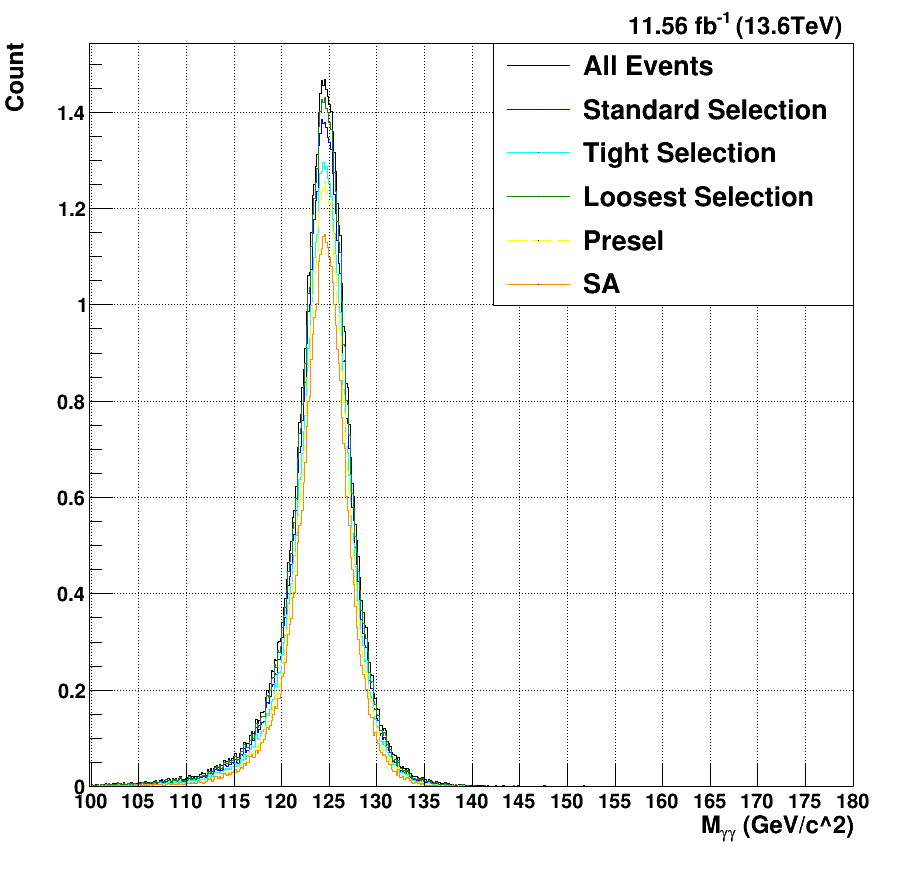
\includegraphics[width=\linewidth]{./Figures/Offline Selection Plots/DiHiggs/0715_FullOfflineCuts_SingleSquarePlots/hggMass_All_Sig.png}
		\caption{Signal MC $M_{\gamma \gamma}$}
		\label{DiHiggsSig:OfflineAcceptance:Mgg}
	\end{subfigure}\hfill
	\begin{subfigure}{0.50\linewidth}
		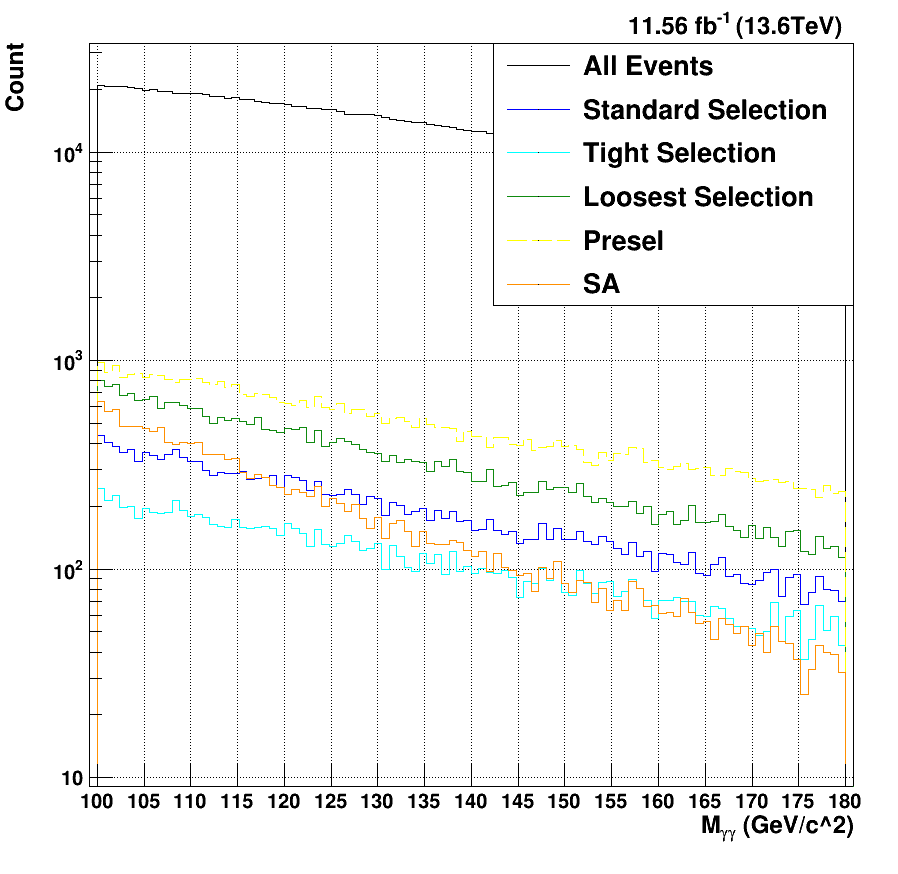
\includegraphics[width=\linewidth]{./Figures/Offline Selection Plots/DiHiggs/0715_FullOfflineCuts_SingleSquarePlots/hggMass_All_Bkg.png}
		\caption{Data $M_{\gamma \gamma}$}
		\label{DiHiggsBkg:OfflineAcceptance:Mgg}
	\end{subfigure}
	\caption{Total offline selection acceptances for $HH \rightarrow b \bar{b} \gamma \gamma$. Three tightnesses of BDT-based selection cuts are shown in dark blue (standard), light blue (tighter), and light green (looser). The acceptance of the preselection is shown in yellow, while the full standard analysis cuts are shown in orange.}
	\label{fig:DiHiggs:OfflineAcceptance:Mgg}
\end{figure}

The $\eta_{SC}$ distributions in figure \ref{fig:DiHiggs:OfflineAcceptance:ScEta} also show similar features to those of the single Higgs. Though the overall proportion of the diHiggs in the endcaps is lower, there is still an enhancement in the kinematic coverage around the low-$\eta$ boundary of the endcap relative to the SA cuts. All three of the BDT-based selections keep consistent efficiency through the whole selected range of $\eta_{SC}$. The data distributions also mirror those of the single Higgs; while the SA cuts show relatively flat acceptance across the whole ECal, the BDT-based selections prefer more central events and cut out photons near the extreme $\eta$ values.

\begin{figure}[H]
	\begin{subfigure}{0.50\linewidth}
		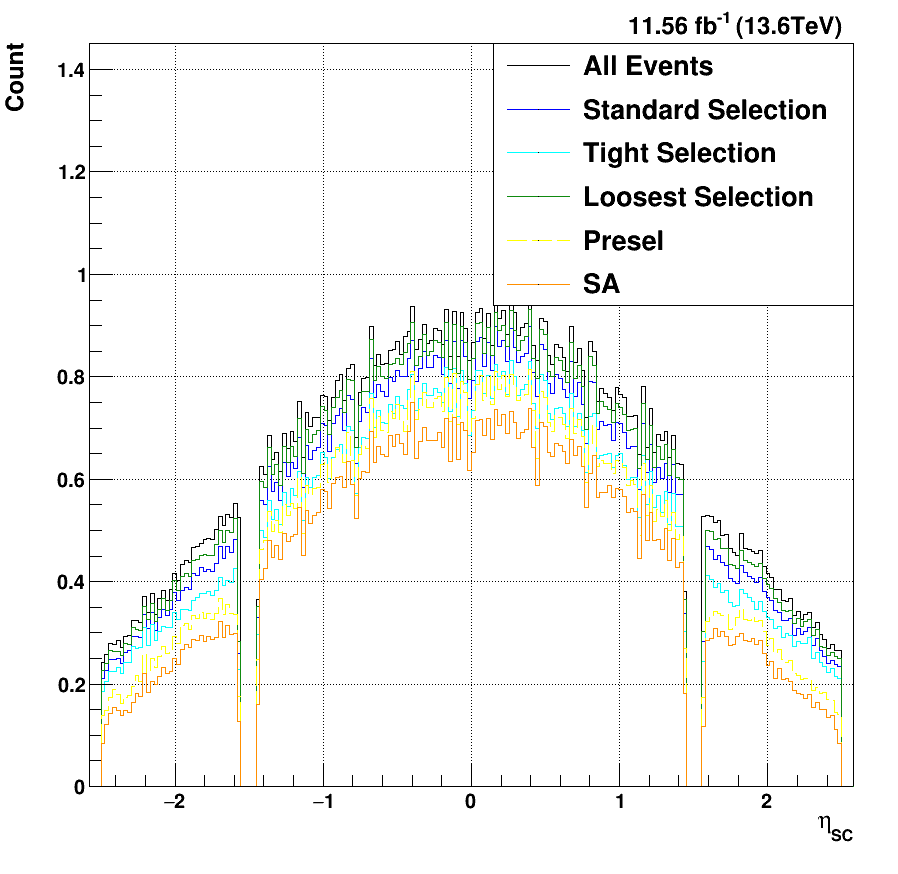
\includegraphics[width=\linewidth]{./Figures/Offline Selection Plots/DiHiggs/0715_FullOfflineCuts_SingleSquarePlots/scEta_All_Sig.png}
		\caption{Signal MC $\eta_{SC}$}
		\label{DiHiggsSig:OfflineAcceptance:ScEta}
	\end{subfigure}\hfill
	\begin{subfigure}{0.50\linewidth}
		\includegraphics[width=\linewidth]{./Figures/Offline Selection Plots/DiHiggs/0715_FullOfflineCuts_SingleSquarePlots/scEta_All_Bkg.png}
		\caption{Data $\eta_{SC}$}
		\label{DiHiggsBkg:OfflineAcceptance:ScEta}
	\end{subfigure}
	\caption{Total offline selection acceptances for $HH \rightarrow b \bar{b} \gamma \gamma$. Three tightnesses of BDT-based selection cuts are shown in dark blue (standard), light blue (tighter), and light green (looser). The acceptance of the preselection is shown in yellow, while the full standard analysis cuts are shown in orange. Both the lead and sublead photons are plotted together.}
	\label{fig:DiHiggs:OfflineAcceptance:ScEta}
\end{figure}

The $p_T/M_{\gamma\gamma}$ distributions in figure \ref{fig:DiHiggs:OfflineAcceptance:PtOvrM} show similar features to those of the single Higgs. The loss of signal efficiency from the explicit $p_T/M_{\gamma\gamma}$ cuts can cleary be seen in figure \ref{DiHiggsSig:OfflineAcceptance:PtOvrM}, while the power of these cuts to reduce the background acceptance can also be seen in figure \ref{DiHiggsBkg:OfflineAcceptance:PtOvrM}.

\begin{figure}[H]
	\begin{subfigure}{0.50\linewidth}
		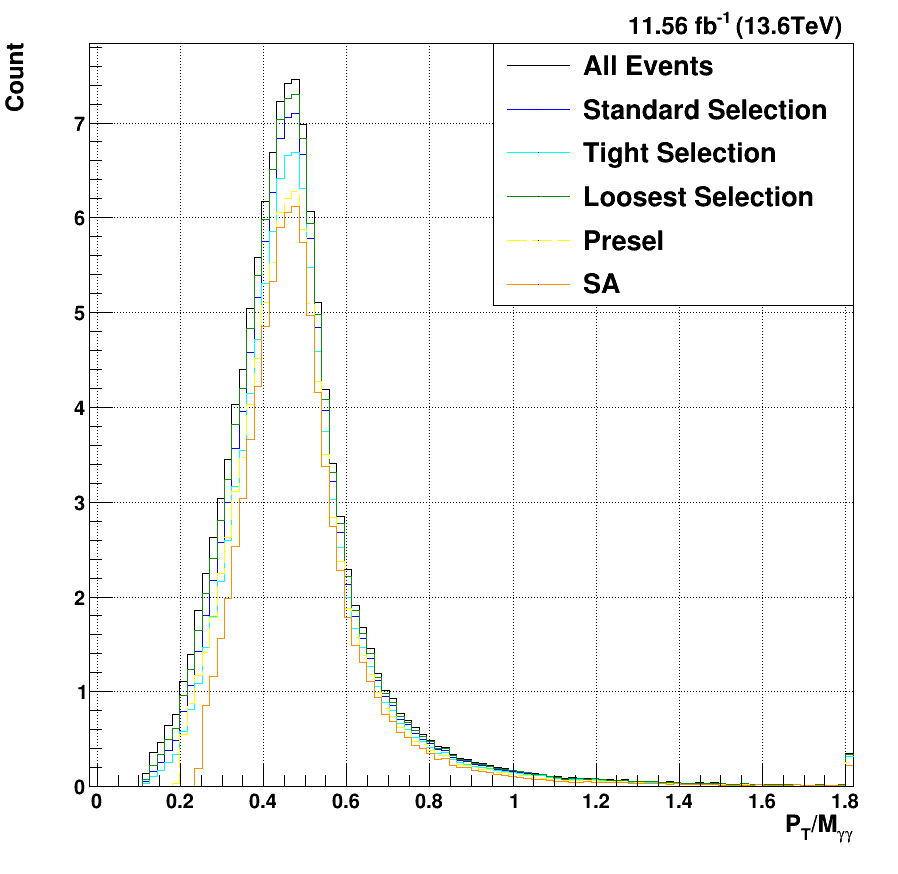
\includegraphics[width=\linewidth]{./Figures/Offline Selection Plots/DiHiggs/0715_FullOfflineCuts_SingleSquarePlots/ptOvrM_All_Sig.png}
		\caption{Signal MC $p_T/M_{\gamma\gamma}$}
		\label{DiHiggsSig:OfflineAcceptance:PtOvrM}
	\end{subfigure}\hfill
	\begin{subfigure}{0.50\linewidth}
		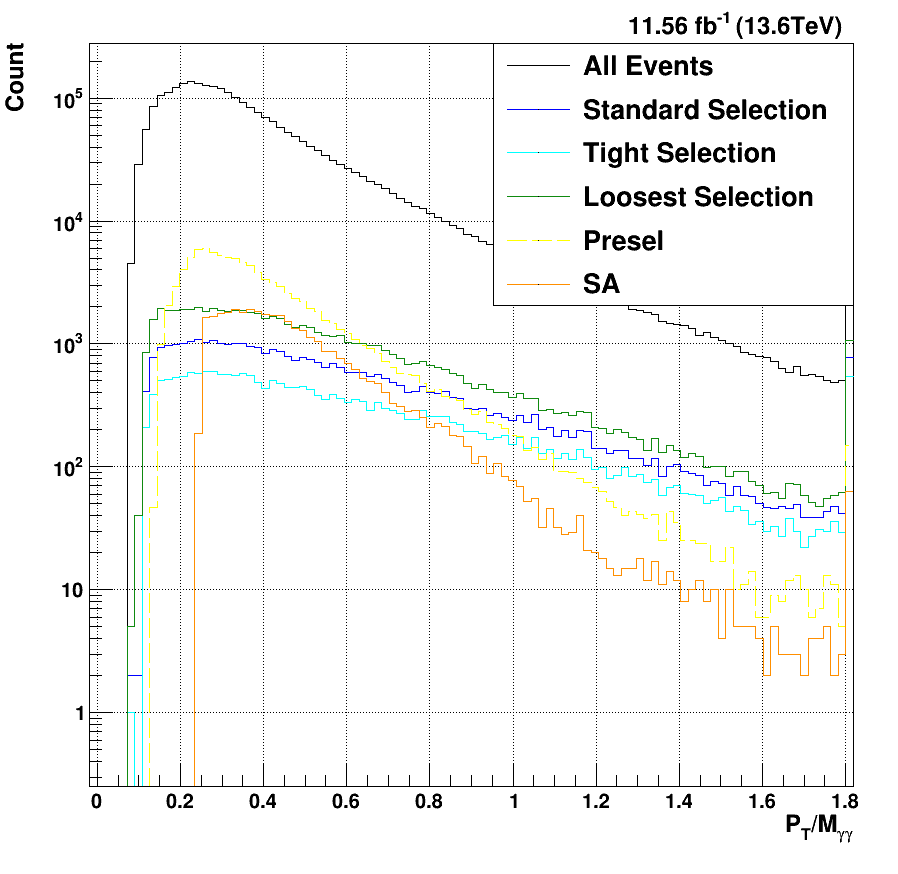
\includegraphics[width=\linewidth]{./Figures/Offline Selection Plots/DiHiggs/0715_FullOfflineCuts_SingleSquarePlots/ptOvrM_All_Bkg.png}
		\caption{Data $p_T/M_{\gamma\gamma}$}
		\label{DiHiggsBkg:OfflineAcceptance:PtOvrM}
	\end{subfigure}
	\caption{Total offline selection acceptances for $HH \rightarrow b \bar{b} \gamma \gamma$. Three tightnesses of BDT-based selection cuts are shown in dark blue (standard), light blue (tighter), and light green (looser). The acceptance of the preselection is shown in yellow, while the full standard analysis cuts are shown in orange. Both the lead and sublead photons are plotted together.}
	\label{fig:DiHiggs:OfflineAcceptance:PtOvrM}
\end{figure}

The overall $HH \rightarrow b \bar{b} \gamma \gamma$ signal MC efficiencies and data acceptances can be seen in table \ref{tab:DiHiggs:offlineTotalEffs}. As with the single Higgs sample, considerable gains are measured accross the whole detector. A particular enhancement is still seen in B-E events, where a relative 64.2\% gain is seen. These massive gains in both the kinematic coverage and the overall signal efficiency should prove a major boon to future diHiggs analyses, and demonstrate the possible power of leveraging the MVA-HLT for future analyses.

\begin{table}[h]
    \centering
    \caption{$HH \rightarrow b \bar{b} \gamma \gamma$ signal efficiencies and background acceptances for both offline selections, broken down by the location of each photon candidate in $\eta_{sc}$}
	\label{tab:DiHiggs:offlineTotalEffs}
    \begin{subtable}{.49\textwidth}
        \centering
        \caption{Signal Efficiencies}
        \begin{tabular}{|c|c|c|c|}
            \hline
            \textbf{Region} & \textbf{BDT(\%)} & \textbf{SA(\%)}& \textbf{Gain(\%)}\\
			\Xhline{2pt}
            B-B & 97.23 & 73.43 &+32.4\\ \hline
            B-E & 88.38 & 53.83 &+64.2\\ \hline
            E-E & 89.88 & 57.02 &+57.6\\ \hline
            All & 94.68 & 67.78 &+39.7\\ \hline
        \end{tabular}
    \end{subtable}
    \hfill
	\begin{subtable}{.49\textwidth}
        \centering
        \caption{Data Acceptances}
        \begin{tabular}{|c|c|c|c|}
            \hline
            \textbf{Region} & \textbf{BDT(\%)} & \textbf{SA(\%)} & \textbf{Gain(\%)}\\
			\Xhline{2pt}
            B-B & 3.12 & 2.42 &+28.9\\ \hline
            B-E & 0.76 & 0.86 &-11.6\\ \hline
            E-E & 1.50 & 1.71 &-12.3\\ \hline
            All & 1.46 & 1.46 &0.0\\ \hline
        \end{tabular}
    \end{subtable}
\end{table}

\chapter{Summary}

\chapter{Acknowledgements}


\appendix
Appendix

% Stuff at the end of the dissertation goes in the back matter
\backmatter
\printbibliography
\end{document}
